% ====================================================================

% LSST Observing Strategy White Paper

% Copyright 2015 The LSST Science Collaborations

% ====================================================================

\documentclass[11pt,headsepline,cleardoubleempty,twoside,openright]{scrbook}
% 11pt font
% Draw a line under the header
% Don't draw a line or print page numbers when a page is empty
% Pages are two-sided - so margins alternate
% Chapters start on the righthand side of the page

\usepackage{LSST_Observing_Strategy_White_Paper}

% ====================================================================

\begin{document}

\begin{titlepage}
\begin{center}

\vspace*{\stretch{3}}

{\Huge\bfseries\scshape
 Science Driven Optimization \\ \vspace{\baselineskip}
 of the LSST Observing Strategy}

\vspace*{\stretch{2}}

% Version number, to be taken out for published draft

% \include{VersionDate}

% \begin{center}
% {\Large\bf Version 1.0\\
%
% \vspace*{\stretch{0.2}}
%
% November 2009}
% \end{center}

\vspace*{\stretch{2.5}}

{\Large  Prepared by the LSST Science Collaborations,}\\
\vspace*{\stretch{0.15}}
{\Large with contributions from the LSST Project. }\\
\vspace*{\stretch{1}}

\end{center}
\end{titlepage}

% --------------------------------------------------------------------

\tableofcontents
\label{toc}

% --------------------------------------------------------------------
\clearemptydoublepage

\setcounter{chapter}{0}
\chapter*{Preface}
\def\chpname{preface}\label{chp:\chpname}
\addcontentsline{toc}{section}{Preface}
\markboth{}{}

\noindent This is a community white paper outlining various science
cases and the impacts that observing strategy will have on them,
quantified using the Metric Analysis Framework. We will describe
various strategies and tradeoffs that impact the observing cadence
(visit sequence), the current cadence baseline, and future directions
for the optimization of the survey strategy. We aim to publish this
white paper on arXiv, and invite community feedback.

The timescale for producing this white paper, started before and
finished after the Observing Strategy workshop at the  August 2015
LSST Project and Community workshop, is many months.

% --------------------------------------------------------------------

\section*{Messages}
% \addcontentsline{toc}{subsection}{Messages}

The main points we will aim to convey in this white paper are as follows:

\begin{itemize}

    \item We have a pretty good idea of how we would deploy LSST:
    there is a baseline strategy and example cadences, with which it
    can be demonstrated that the data required for the promised
    science can be delivered.

    \item The baseline strategy can and will be optimized -- even small
    improvements can be significant. Most importantly, the strategy is
    not set in stone and it will evolve.

    \item The cadence optimization process will be as open and
    inclusive as technically possible. All stakeholders will
    participate in this process.

\end{itemize}

\raggedright{Project start: July 2015.}

% --------------------------------------------------------------------

\section{Guidelines for Authors}
% \addcontentsline{toc}{section}{Guidelines for Authors}
\def\secname{guidelines}\label{sec:\secname}

\noindent{\it Phil Marshall}
%(\texttt{@drphilmarshall})

Since this is a community white paper, contributions are welcome from
everyone. Read on for how to make a contribution, and how you should
structure that contribution.\footnote{These notes on the white paper
design are pasted from \texttt{whitepaper/notes/chapter-template.md}}


\subsection{How to get involved}

The first thing you should do is read and absorb the current version
of the white paper, which you should be able to
\href{http://ls.st/iw2}{view on \GitHub}. You will then be able to
provide good feedback, which you should do via the
\href{https://github.com/LSSTScienceCollaborations/ObservingStrategy/issues}{\GitHub
issues}. Browse the existing issues first: there might be a
conversation you can  join. New issues are most welcome: we'd like to
make this white paper as comprehensive as possible.

To edit the white paper, you'll need to
\href{https://help.github.com/articles/fork-a-repo/}{``fork'' its
repository}. You will then  be able to edit the paper in your own
fork, and when you are ready,  submit a
\href{https://help.github.com/articles/using-pull-requests/}{``pull
request''} explaining what you are doing and the new version that  you
would like to be accepted. It's a good idea to submit this pull
request sooner rather than later, because associated with it will be a
discussion thread that the writing community can use to discuss your
ideas with you. For help getting started with \git and \GitHub, please
see this
\href{https://github.com/drphilmarshall/GettingStarted#top}{handy
guide}.


\subsection{Chapter and section design}

The first section of each science chapter needs to be an {\it introduction}
that outlines, very briefly, the commonality of the key science cases
contained in it:  what is to be measured, in broad-brush terms, and
why this is of interest. Then, suppose we were to design an LSST
survey to enable these measurements: qualitatively, what might it look
like, in terms of the choices we are able to make? This chapter
introduction can eventually (when the results are in!) summarize,
again, in very broad brush terms, the results of a number of
investigative sections, one on each science case.

The individual sections following this introduction will need to
describe the particular discoveries and measurements that are being
targeted in each {\it science case}. It will be helpful to think of a
``science case" as a ``science project" that the section leads {\it
actually plan to do}. Thinking this way means that the sections can
follow the tried and tested format of an observing proposal: a brief
description of the investigation, with references, followed by a
technical feasibility piece.  This latter part will need to be
quantified using the MAF framework, via a set of metrics that need to
be computed for any given observing strategy to quantify its impact on
the described science case. Ideally, these metrics would be combined
in a well-motivated figure of merit. The section can conclude with a
discussion of any risks that have been identified, and how these could
be mitigated.

The following two sections are an example chapter introduction and
science case section for you to work from. The latter is checked into
the repository as \texttt{section-template.tex}.

% --------------------------------------------------------------------

\section{Example Introduction}

General introduction to the chapter's science projects.

Overview of observing strategy needed by those projects, bringing
out common themes or points of tension.

% --------------------------------------------------------------------

% ====================================================================
%+
% SECTION:
%    section-name.tex  % eg lenstimedelays.tex
%
% CHAPTER:
%    chapter.tex  % eg cosmology.tex
%
% ELEVATOR PITCH:
%    Explain in a few sentences what the relevant discovery or
%    measurement is going to be discussed, and what will be important
%    about it. This is for the browsing reader to get a quick feel
%    for what this section is about.
%
% COMMENTS:
%
%
% BUGS:
%
%
% AUTHORS:
%    Phil Marshall (@drphilmarshall)  - put your name and GitHub username here!
%-
% ====================================================================

\section{ Title of Science Project }
\def\secname{keyword}\label{sec:\secname} % For example, replace "keyword" with "lenstimedelays"

\noindent{\it Author Name(s)} % (Writing team)

% This individual section will need to describe the particular
% discoveries and measurements that are being targeted in this section's
% science case. It will be helpful to think of a ``science case" as a
% ``science project" that the authors {\it actually plan to do}. Then,
% the sections can follow the tried and tested format of an observing
% proposal: a brief description of the investigation, with references,
% followed by a technical feasibility piece. This latter part will need
% to be quantified using the MAF framework, via a set of metrics that
% need to be computed for any given observing strategy to quantify its
% impact on the described science case. Ideally, these metrics would be
% combined in a well-motivated figure of merit. The section can conclude
% with a discussion of any risks that have been identified, and how
% these could be mitigated.

A short preamble goes here. What's the context for this science
project? Where does it fit in the big picture?

% --------------------------------------------------------------------

\subsection{Target measurements and discoveries}
\label{sec:keyword:targets}

Describe the discoveries and measurements you want to make.

Now, describe their response to the observing strategy. Qualitatively,
how will the science project be affected by the observing schedule and
conditions? In broad terms, how would we expect the observing strategy
to be optimized for this science?


% --------------------------------------------------------------------

\subsection{Metrics}
\label{sec:keyword:metrics}

Quantifying the response via MAF metrics: definition of the metrics,
and any derived overall figure of merit.


% --------------------------------------------------------------------

\subsection{OpSim Analysis}
\label{sec:keyword:analysis}

OpSim analysis: how good would the default observing strategy be, at
the time of writing for this science project?


% --------------------------------------------------------------------

\subsection{Discussion}
\label{sec:keyword:discussion}

Discussion: what risks have been identified? What suggestions could be
made to improve this science project's figure of merit, and mitigate
the identified risks?


% ====================================================================

\navigationbar


% --------------------------------------------------------------------


% --------------------------------------------------------------------


\chapter[Introduction]{Introduction}
\def\chpname{intro}\label{chp:\chpname}

Chapter editors:
\credit{bethwillman},
\credit{connolly}.

The Large Synoptic Survey Telescope (LSST) is a dedicated optical
telescope with an effective aperture of 6.7 meters, currently under
construction on Cerro Pach\'on in the Chilean Andes.  The telescope
and camera will have a huge field of view, 9.6 deg$^2$, and the
\'etendue, i.e., the product of collecting area and field of view will
be significantly larger than any other telescope.  Thus this telescope
is designed for wide-field deep imaging of the sky; its mantra is
``Wide-Deep-Fast'', i.e., the ability to cover large swaths of sky
(``Wide'') to faint magnitudes (``Deep'') in a short amount of time
(``Fast''), allowing to scan the sky repeatedly.

  The science case for the LSST is based broadly on four science
  themes:
\begin{itemize}
\item Dark energy and dark matter (via strong and weak lensing,
  large-scale structure, and supernovae);
\item Exploring the transient and variable universe;
\item Studying the structure of the Milky Way galaxy and its neighbors
  via resolved stellar populations;
\item An inventory of the Solar System, including Near-Earth Asteroids
  and Potential Hazardous Objects, Main-Belt Asteroids, and
  Kuiper-Belt Objects.
\end{itemize}

These themes, together with {\em many} other science applications, are
described in detail in the
\href{http://lsst.org/scientists/scibook}{LSST Science Book}, produced
by the LSST Project Team and Science collaborations in 2009.  The
present white paper represents an important next step in science
planning beyond the Science Book.  In particular, we now need to
quantify how well the LSST (for a given realization of its cadence)
will be able to carry out its science goals; indeed, we will use this
quantification to refine and optimize the cadence itself.

The Science Book is six years old.  In those six years, some of the
science themes described in there have evolved or become obselete,
while new science opportunities and ideas have arisen.  Moreover, our
understanding of the capabilities (such as system response and
therefore depth, telescope optics, and so on) have matured
considerably.  The present document endeavors to explore the
principal science themes as described in the Science Book, but is not
slaved to them, and where appropriate, we will point out relevant
updates to the Science Book.


% --------------------------------------------------------------------

\section{Synoptic Sky Surveying at Universal Cadence}
\def\secname{intro:baseline}\label{sec:\secname}

Synoptic Surveying with LSST - the basic observing strategy determined
by key projects described in the LSST Science Requirements Document,
and constrained by the LSST's design \citep{IvezicEtal2008}.

% --------------------------------------------------------------------

\section{Beyond the Baseline Observing Strategy}
\def\secname{intro:baseline}\label{sec:\secname}

Optimizing the Observing Strategy: what perturbations are we
permitted to introduce, to maximize the system's science capabilities?
What are our constraints? And our opportunities?

% --------------------------------------------------------------------

\section{Evaluation and Optimization of the LSST Observing Strategy}
\def\secname{intro:evaluation}\label{sec:\secname}

The first step towards a science-based optimization of the LSST
observing strategy is a {\it science-based evaluation of the baseline
LSST observing strategy}. After simulating a sample  observing
schedule consistent with this strategy (see  \autoref{chp:cadexp}), we
then need to quantify its value to each science team. This is what the
LSST DM Sims team's ``Metric Analysis Framework''  was designed to
enable. Once the fiducial strategy has been evaluated in this way,
then any other strategy can be evaluated in the same terms, using the
same code, and we will be able to start optimizing the strategy
through iterations between \OpSim and MAF.

With this program in mind, it makes sense to define {\it one ``Figure
of Merit'' (FoM) per science project}, that captures the value of  the
observing strategy under consideration to that science team. This FoM
will probably be a function of several ``metrics'' that quantify
lower-level features of the observing sequence.  For Figures of Merit
to be directly comparable between disparate science projects,  they
need to be dimensional, and have the same units. One natural
choice could be the {\it information gained} by the science team, in
bits. This is a well-defined statistical quantity, albeit not yet one
in common use. A given observing schedule's value would then depend on
both this information gain, but also {\it how much that information is
worth to the whole community}. It is at this point that the debate
could become heated: probably the best we can do in Cadence Diplomacy
is to quantify all the information gains implied by each proposed
change to the baseline  observing strategy, combine them to see
whether it makes everyone happy, and iterate. In this way we might
hope to minimize the debates about the less quantifiable worth of each
piece of information.

We are some way from being able to define information-based Figures of
Merit for most science cases -- but the metrics that they will depend
on will be easier to derive. Writing this white paper is an
opportunity to think through the Figure of Merit for each science
project that we as a community want to carry out, and how that measure
of success is likely (or even known) to depend on metrics that
summarize the observing sequence presented to us. Thinking about the
problem in terms of science projects, each with a  Figure of Merit,
encourages us to design modular document sections, with one science
project and one Figure of Merit per section.

This will have the happy side-effect of allowing the chapters to be
straightforwardly re-arranged as we go, to make the white paper easier
to read. It will also naturally lead to the definition of a suite of
MAF  super-metrics, can be evaluated on any future \OpSim output
database.  A table in each section showing the values of the metrics
and the FoM, for different schedules, for that science project, will
be very helpful. The metric names in these tables should match the
metric class names in the
\href{https://github.com/LSST-nonproject/sims_maf_contrib/wiki}{\simsMafContrib}
module. In principle these tables could be auto-generated by the MAF
framework, and extended as \OpSim is repeatedly reconfigured and run.

For an example of how all this could look, please see the
\hyperref[sec:lenstimedelays]{lens
time delays section}. The MAF subsections are still under development
there, but keep checking back to see it come together during the
August 2015 workshop week. Templates for the chapters and sections can
be found in \autoref{chp:example}.


% --------------------------------------------------------------------

\section{Outline of This Paper}
\def\secname{intro:outline}\label{sec:\secname}

The rest of this white paper is structured as follows. In
\autoref{chp:cadexp} we describe a number of \OpSim simulated observing
schedules (``cadences'') explored by the LSST Sims team in summer 2015
in preparation for this paper: they include a ``baseline cadence'', and
then some small but interesting perturbations to it. Then, we present
the science cases considered so far, organised into the following
chapters:

\begin{itemize}
    \item \autoref{chp:solarsystem}: \nameref{chp:solarsystem}
    \item \autoref{chp:galaxy}: \nameref{chp:galaxy}
    \item \autoref{chp:astrometry}: \nameref{chp:astrometry}
    \item \autoref{chp:variables}: \nameref{chp:variables}
    \item \autoref{chp:transients}: \nameref{chp:transients}
    \item \autoref{chp:cosmo}: \nameref{chp:cosmo}
    \item \autoref{chp:deepdrilling}: \nameref{chp:deepdrilling}
    \item \autoref{chp:specialsurveys}: \nameref{chp:specialsurveys}
\end{itemize}

Finally, in \autoref{chp:tradeoffs} we bring the results of all the
science metric analyses  together and discuss the tensions between
them, and the trade-offs that we can anticipate having to make.

\navigationbar

% --------------------------------------------------------------------


% --------------------------------------------------------------------

% --------------------------------------------------------------------

\chapter[Some Example Observing Strategies]{Some Example Observing Strategies}
\def\chpname{cadexp}\label{chp:\chpname}

\noindent {\it
LSST Simulations Team, LSST Project Science Team, and Other Contributors
}

% --------------------------------------------------------------------

\noindent{\bf Summary:} In this chapter (which was originally prepared
as the standalone report available from
\url{http://www.astro.washington.edu/users/ivezic/lsst/cadexp2.pdf})
we analyze and compare the performance of a number of simulated LSST
observing strategies (``cadences'')
which were developed in support of the LSST 2015 Observing
Strategy Workshop.  A candidate new Baseline Cadence,
\opsimdbref{db:enigma}, was found adequate and is proposed as  a
replacement for the previous Baseline Cadence (\texttt{opsim3.61}).
Simulations that only implemented Universal
Cadence proposal imply a margin of about 40\% relative to the design
specifications for the main survey sky coverage and the number of
visits per field from the Science Requirements Document. This margin
can be used to increase the sky coverage of the main survey, the total
number of visits per field, or to implement special programs, such as
deep drilling fields and Galactic plane coverage. Several  simulations
analyzed here quantitatively explore these strategic options.
Additional simulations show that the effects of variations of the
visit exposure time in the  range 20-60 seconds on surveying
efficiency can be predicted using simple efficiency estimates. Various
modifications of baseline cadence (e.g. Pan-STARRS-like cadence,  no
visit pairs, sequences with 3 and 4 visits) indicate a large parameter
space for further optimization, especially for time-domain
investigations and detailed coverage of special sky regions.

% --------------------------------------------------------------------

\section{Introduction}
\def\secname{cadexp:intro}\label{sec:\secname}

With the release of the latest version of Operations Simulations
(hereafter \OpSim) code (version 3.2.1)  for simulating LSST
deployment, and the active development of Metrics Analysis Framework
(\MAF,  currently version 0.2) for analyzing \OpSim outputs, we can
now begin to undertake systematic and  massive investigations of
various LSST deployment strategies.

The optimization of the ultimate LSST observing strategy will be done
with significant input from  the community. To facilitate this
process, the first of a series of meetings, named ``LSST \& NOAO
Observing Cadences Workshop'', was held during the
\href{https://project.lsst.org/meetings/ocw}{LSST 2014 meeting} in
Phoenix, AZ, August 11-15, 2014. The next workshop , named ``LSST
Observing Strategy Workshop'',  will be held
\href{http://lsstsciencecollaborations.github.io/ObservingStrategy/}{after
the LSST 2015 meeting} in Bremerton, WA, August 20-22, 2015.

In part as a preparation for this upcoming workshop, the LSST
Simulations Team and the Project Science Team have designed, executed
and analyzed a number of simulated surveys.  The cadence strategies
for these surveys, while similar to Baseline Cadence, are modified to
study the impact of various strategy variations on the scientific
potential of LSST. The cadence set also includes a candidate baseline
cadence replacement.

An initial analysis of these simulated surveys is presented here.
\href{https://confluence.lsstcorp.org/display/SIM/MAF+documentation}{MAF}
reports for all simulated cadences are available from \begin{verbatim}
http://tusken.astro.washington.edu:8080/?runId=2 \end{verbatim}

\listofopsimdbs

\navigationbar

% --------------------------------------------------------------------

\section{The Baseline Observing Strategy}
\def\secname{cadexp:baseline}\label{sec:\secname}

The current ``official'' (managed by the LSST Change Control Board)
Baseline Cadence, \texttt{opsim3.61},  was produced with an old version of
\OpSim code. We first introduce a candidate replacement simulation
that was produced using  the latest version (v3.2.1) of \OpSim code,
and then proceed with the analysis of other simulations that modify
observing strategy in various informative ways. Suggestions for
further tool development, and a summary of the main cadence questions
addressed  here are available at end of this document.

% - - - - - - - - - - - - - - - - - - - - - - - - - - - - - - - - - -

%%%%%%%%%%%%%%%%%%%%%%%%%%%%%%%%%
\opsimdb[db:enigma]{enigma\_1189}{the new Baseline Cadence.}
%%%%%%%%%%%%%%%%%%%%%%%%%%%%%%%%%

%%%%%%%%%%%%%%%%%%%%%%%%%%%%%%%%%
\begin{figure}[tbh!]
\vskip -1.3in
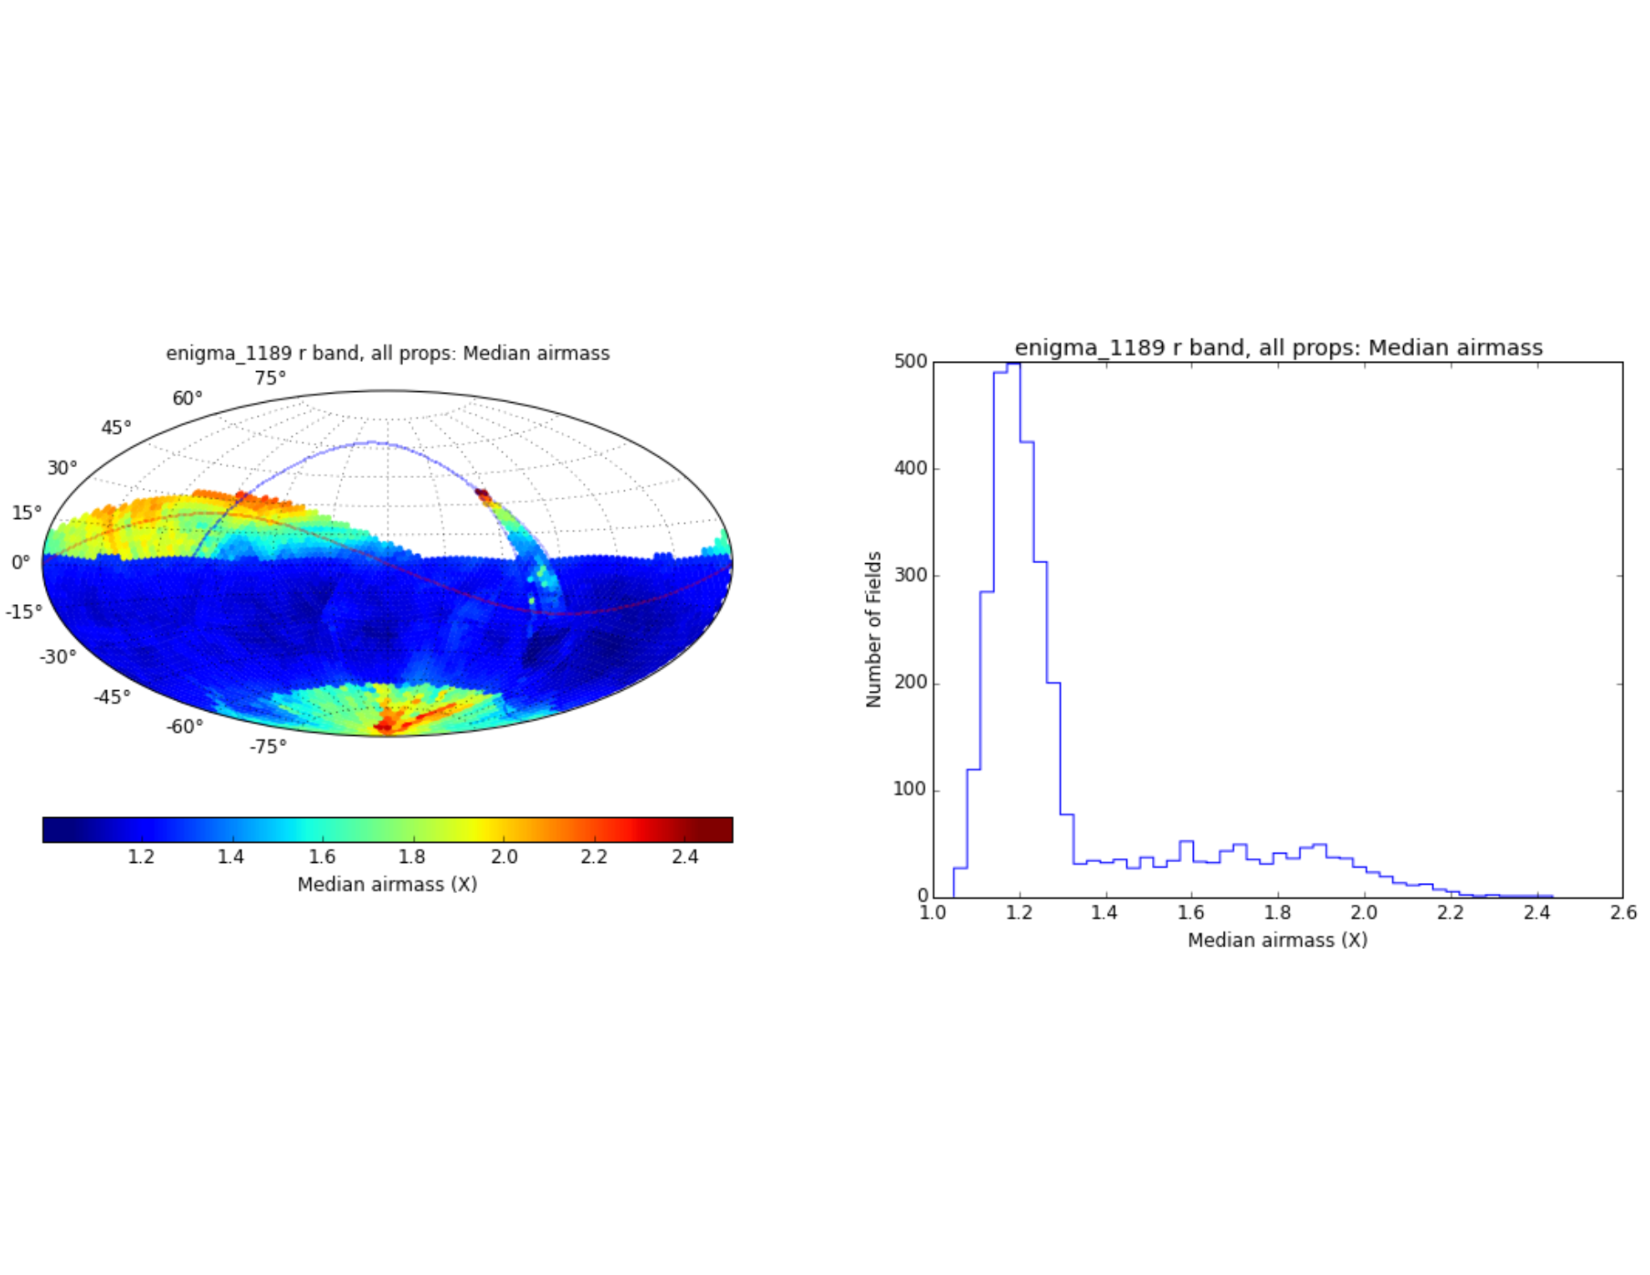
\includegraphics[angle=0,width=0.99\hsize:,clip]{figs/enigma1189_airmass.pdf}
\vskip -1.3in
\caption{The median airmass in the $r$ band across the sky for simulated cadence
\opsimdbref{db:enigma} is shown in Aitoff
projection of equatorial coordinates in the left panel. The corresponding histogram is
shown in the right panel. For the main survey area, the maximum allowed airmass
was set to 1.5. }
\label{fig:airmassenigma}
\end{figure}
%%%%%%%%%%%%%%%%%%%%%%%%%%%%%%%%%

%%%%%%%%%%%%%%%%%%%%%%%%%%%%%%%%%
\begin{figure}[t!]
\vskip -0.1in
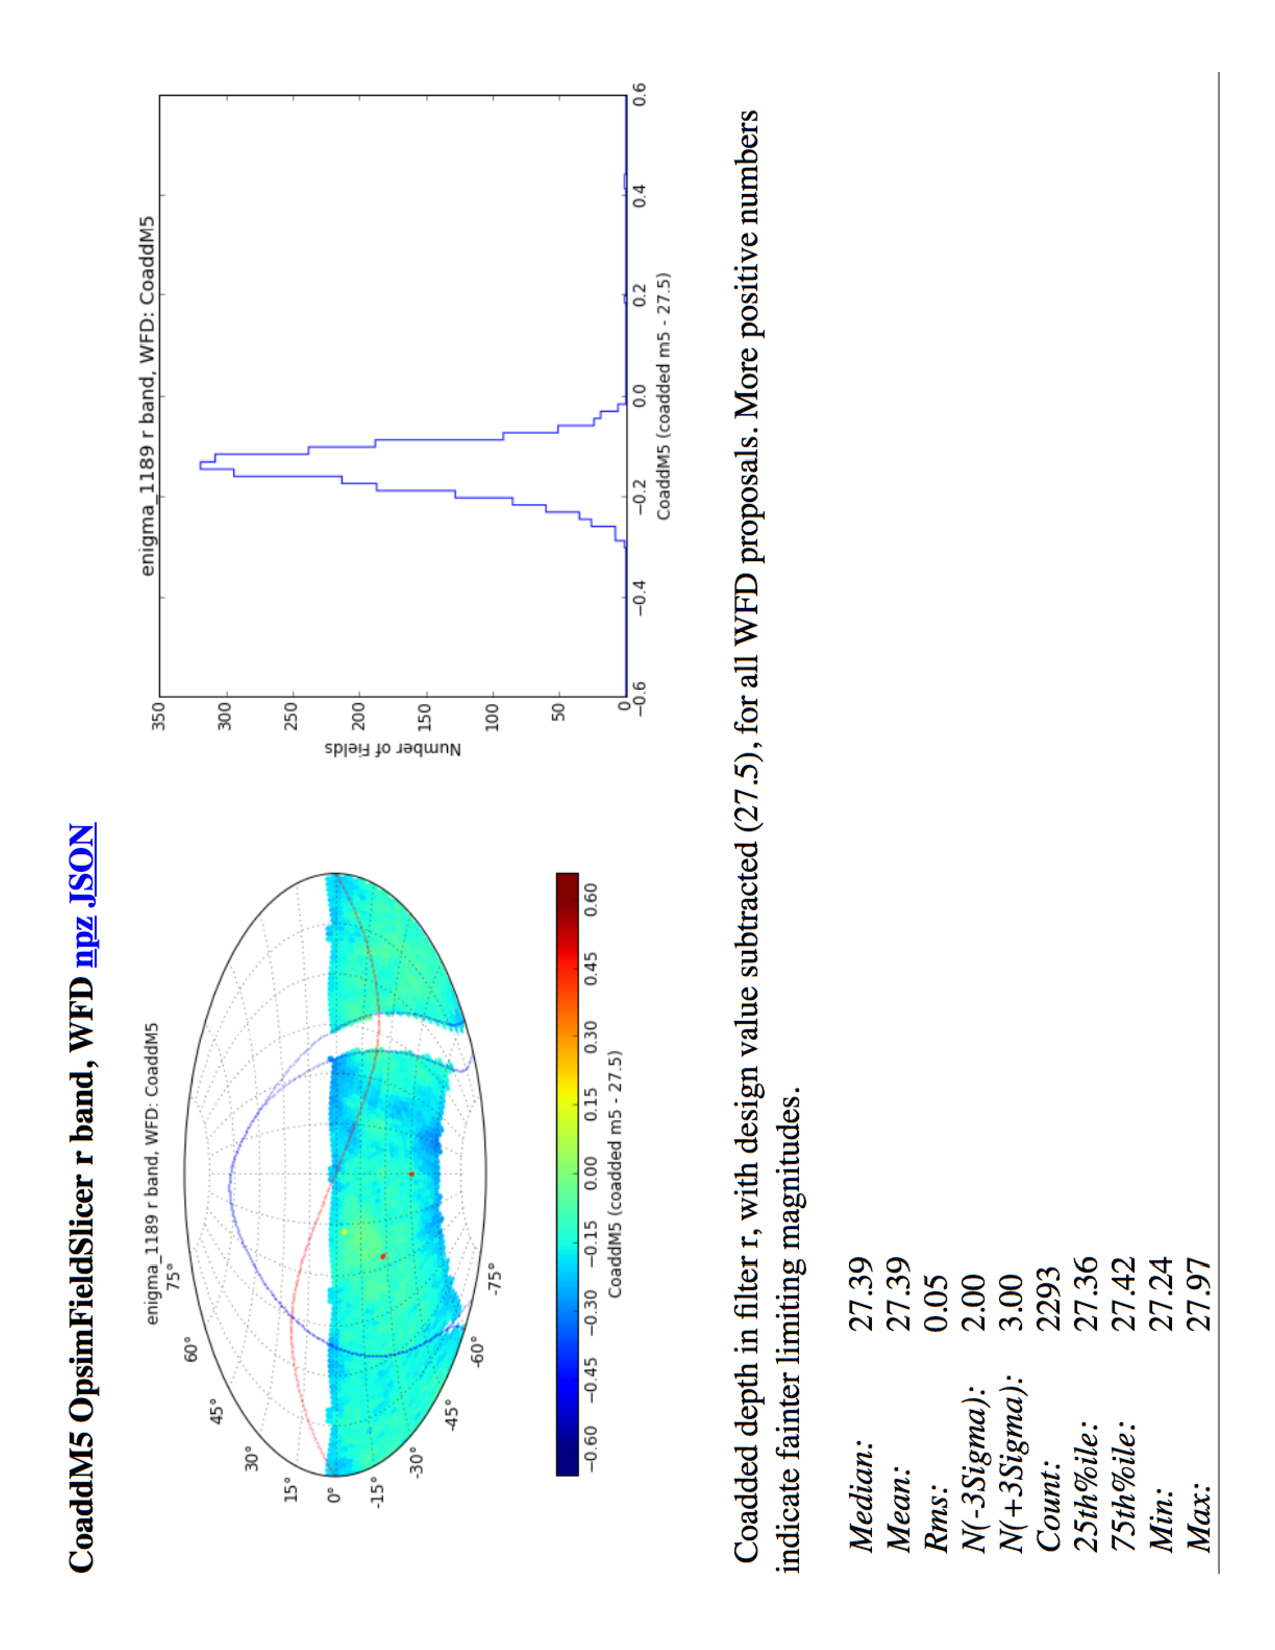
\includegraphics[angle=270,width=0.99\hsize:,clip]{figs/enigma1189_DWFcoaddr5.pdf}
\caption{A screen grab from web-based MAF analysis of simulated cadence
\opsimdbref{db:enigma}. The coadded $5\sigma$ depth for point sources in the $r$ band
across the main survey area (WFD=``wide-fast-deep'') is shown in the top left corner,
in Aitoff projection of equatorial coordinates. The red line shows the Ecliptic and
the blue line shows the Galactic equator (it bifurcates around the so-called
``Galactic confusion zone'').  The distribution of the limiting depth across this
area is shown as a histogram in the top right corner. The basic statistics for
this distribution are listed in the bottom left.}
\label{fig:coaddm5enigma}
\end{figure}
%%%%%%%%%%%%%%%%%%%%%%%%%%%%%%%%%

%%%%%%%%%%%%%%%%%%%%%%%%%%%%%%%%%
\begin{figure}[t!]
\vskip -0.0in
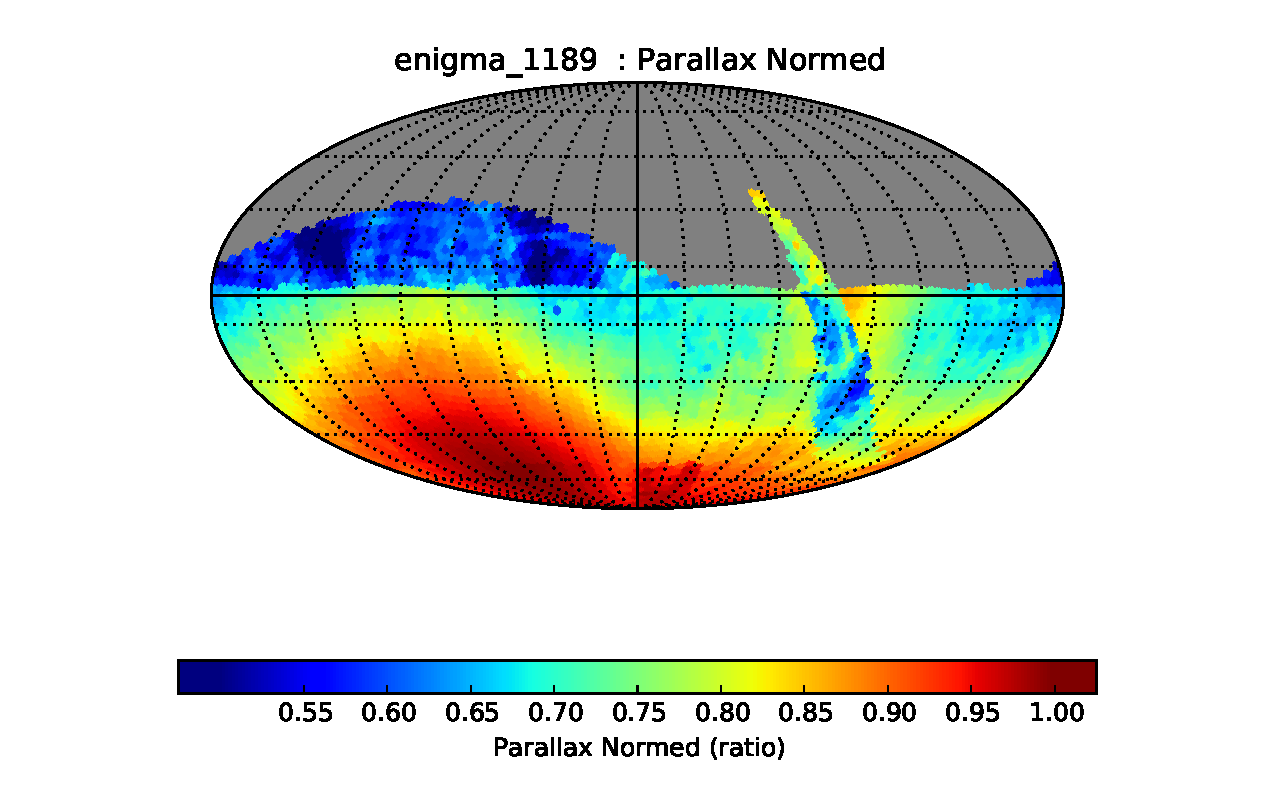
\includegraphics[angle=0,width=0.49\hsize:,clip]{figs/enigma_1189_Parallax_Normed__HEAL_SkyMap.pdf}
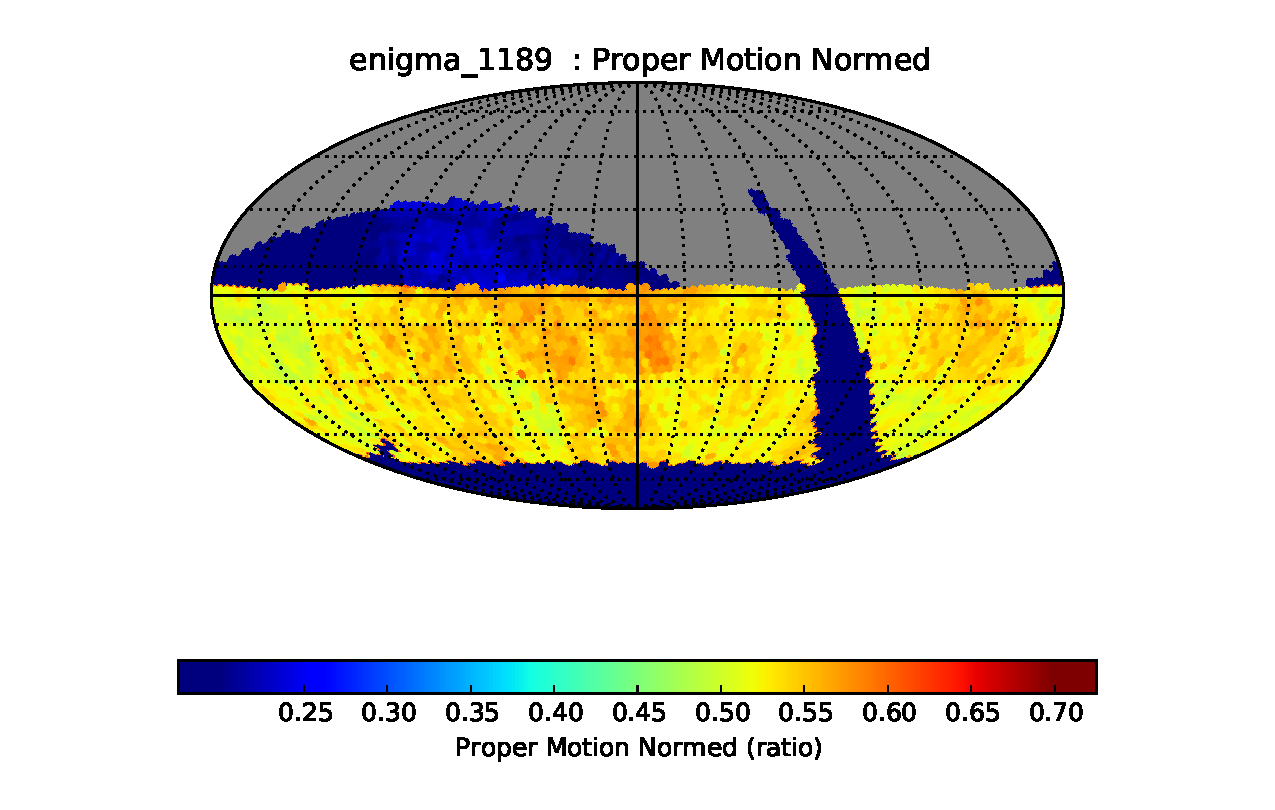
\includegraphics[angle=0,width=0.49\hsize:,clip]{figs/enigma_1189_Proper_Motion_Normed__HEAL_SkyMap.pdf}
\vskip -0.1in
\caption{The trigonometric parallax errors (left) and proper motion errors (right), normalized
by the values for idealized perfectly optimized cadences (parallax: all the observations are taken
at maximum parallax factor, resulting in a peak at the South Ecliptic pole; proper motion:
a half of all visits are obtained on the first day and the rest on the last day of the survey),
obtained for simulated cadence \opsimdbref{db:enigma} are shown in Aitoff projection of equatorial
coordinates.}
\label{fig:parapmenigma}
\end{figure}
%%%%%%%%%%%%%%%%%%%%%%%%%%%%%%%%%

%%%%%%%%%%%%%%%%%%%%%%%%%%%%%%%%%
\begin{figure}[t!]
\vskip -0.2in
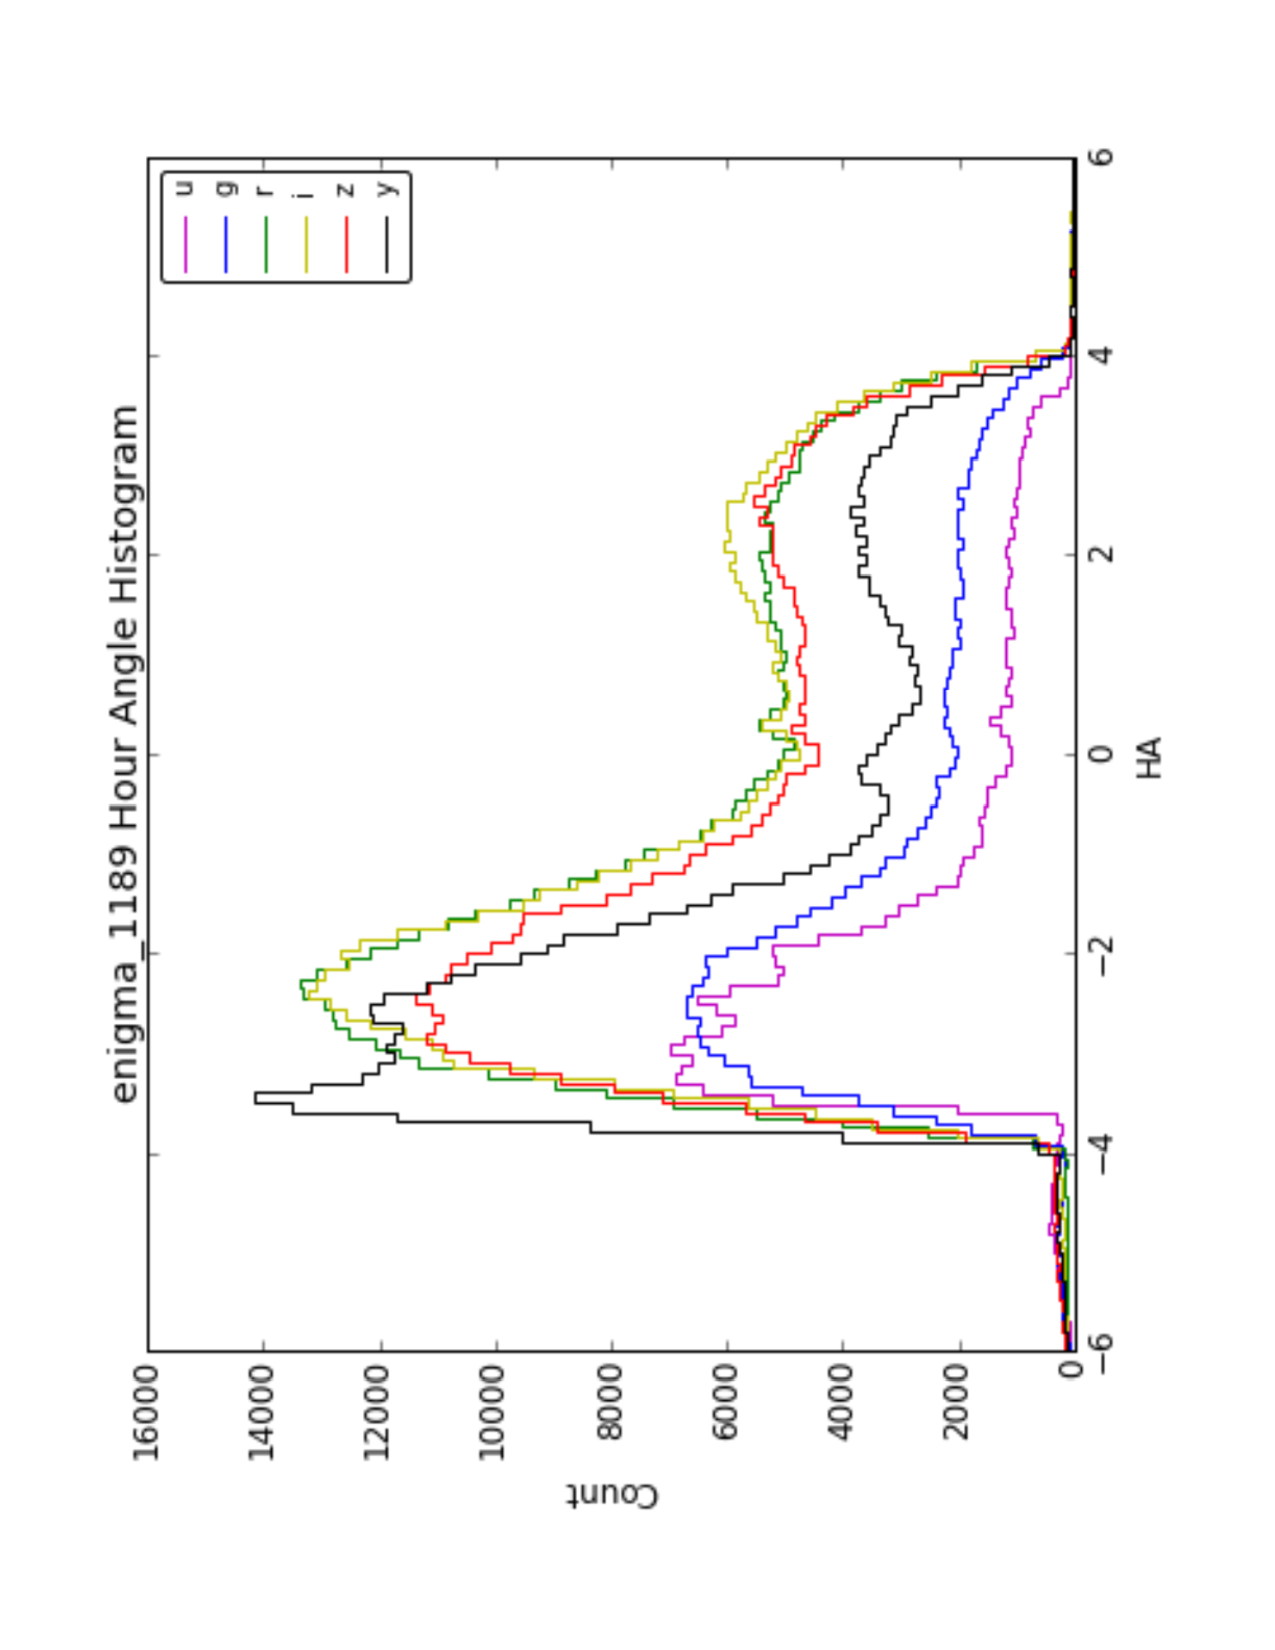
\includegraphics[angle=270,width=0.49\hsize:,clip]{figs/enigma1189_HA.pdf}
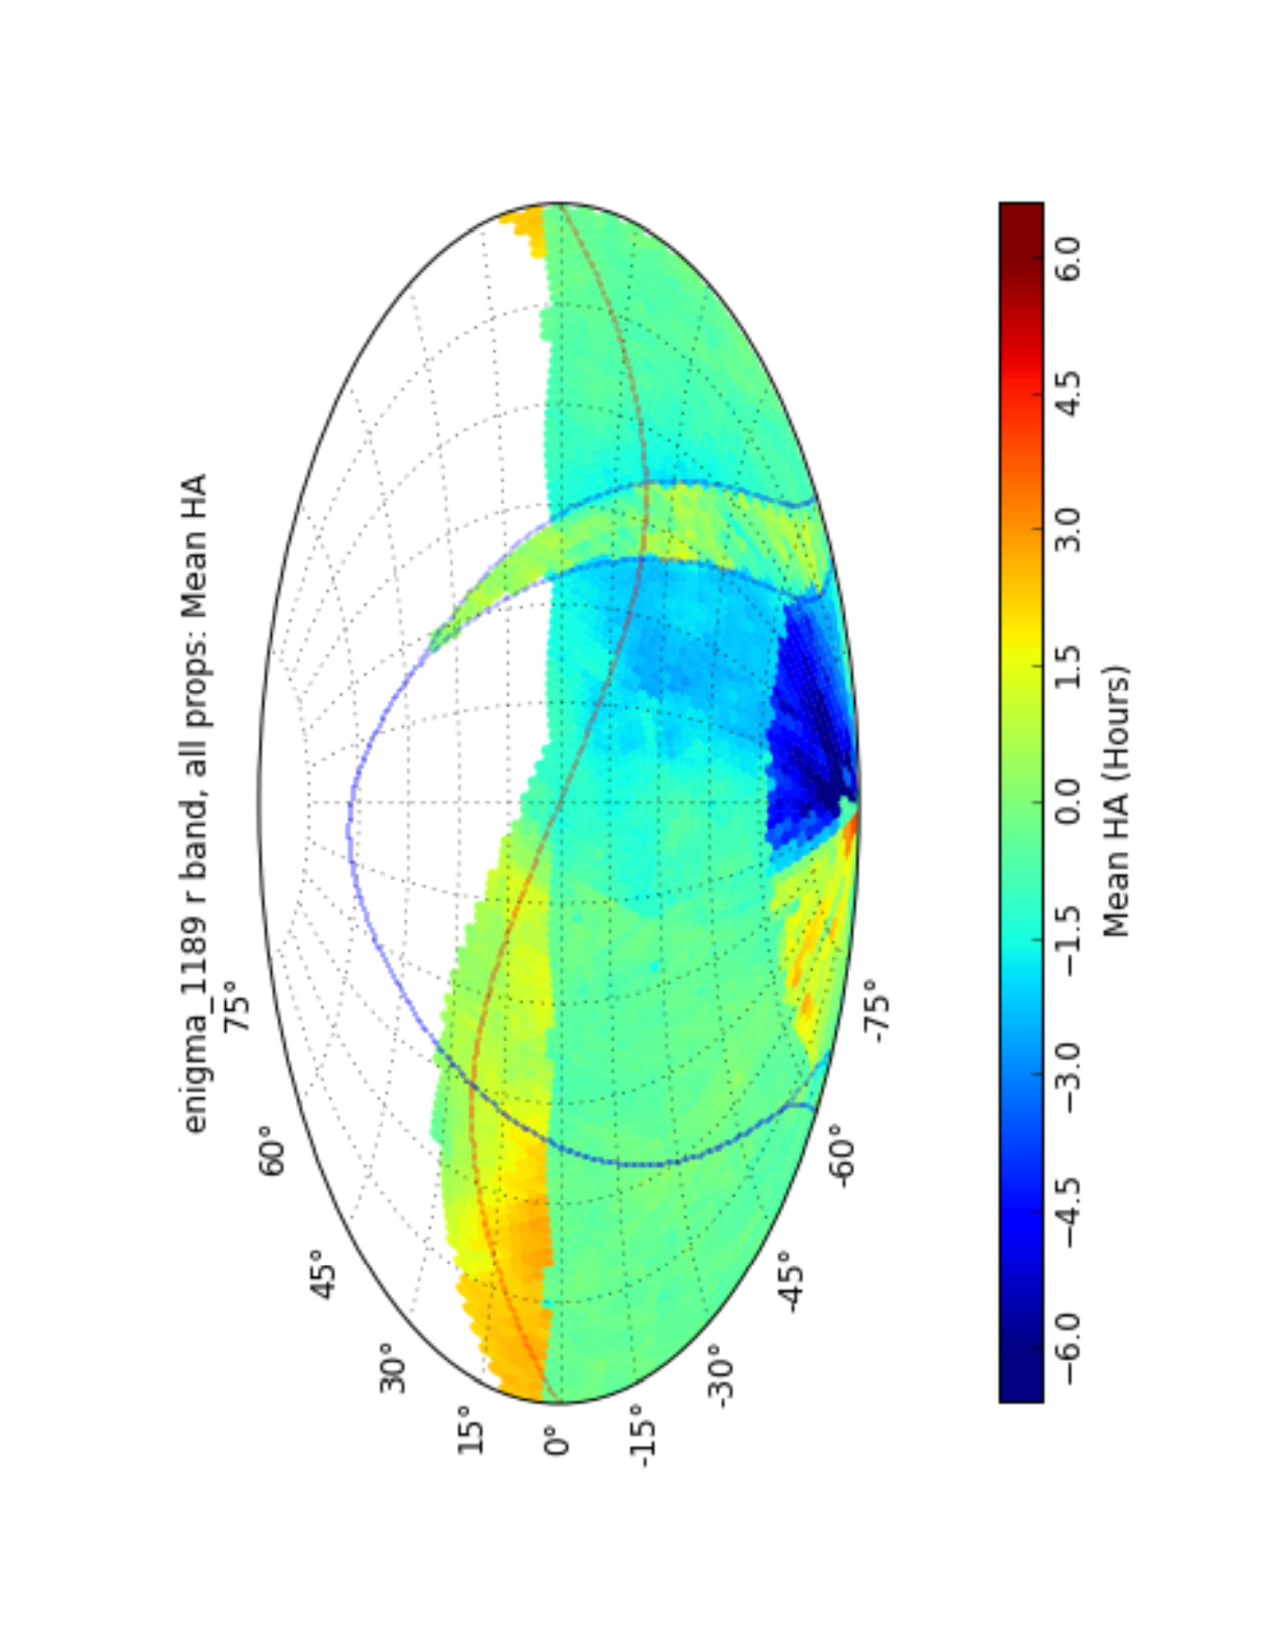
\includegraphics[angle=270,width=0.49\hsize:,clip]{figs/enigma1189_meanHA.pdf}
\vskip -0.3in
\caption{Histograms in the left panel show the distribution of hour angles (HA) in
6 bands for all proposals from simulated cadence \opsimdbref{db:enigma} (the distributions are
similar for WFD fields considered alone). Note the bias towards observations west from
the meridian. The right panel shows the distribution across the sky of the mean HA for
all observations in the $r$ band. }
\label{fig:HAenigma}
\end{figure}
%%%%%%%%%%%%%%%%%%%%%%%%%%%%%%%%%


The candidate replacement ``Baseline Cadence'' candidate,
\opsimdbref{db:enigma}, has the following basic
properties\footnote{See
http://tusken.astro.washington.edu:8080/summaryStats?runId=1}:
\begin{enumerate}
\item The total number of visits is 2,469,307, with 85.4\% spent on
the Universal proposal (the main deep-wide-fast survey), 6.4\% on the
North Ecliptic proposal, 1.7\% on the Galactic plane proposal, 2.1\%
on the South Celestial pole proposal, and 4.5\% on the Deep Drilling
cosmology proposal.
\item The median number of visits {\it per night} is 815, the range is
35 to 1104, with 3062 observing nights. The mean slew time is 6.9
seconds (median: 4.8 sec) and the total open shutter time is 4.06
Msec. The median total open shutter time (per night) as a fraction of
the observing time (the ratio of the open shutter time and the sum of
the open shutter time, readout time and slew time) is 73\%. The
25\%-75\% quartiles for the number of filter changes per night are 2
and 7, with the mean of 4.6. The total number of filter changes is
15,364.
\item In the $r$ band, the median seeing is 0.77 arcsec, the median
airmass is 1.23, and the median $5\sigma$ depth for point sources is
24.5. The variation of the median airmass for the $r$ band
observations with the position on the sky is shown in
\autoref{fig:airmassenigma}.
\item For the 2,293 fields (somewhat overlapping) from the Universal
Cadence area (also known as WFD -- wide, fast, deep), the median
number of visits in the $ugrizy$ bands is (63, 89, 202, 202, 182,
181), respectively. Not only that these medians exceed the requested
number of visits (design specification from the SRD\footnote{The LSST
Science Requirements Document (SRD) is available as
http://ls.st/lpm-17}) of (56, 80, 184, 184, 160, 160) in the $ugrizy$
bands, but the minimum number of visits per field over this area does
so, too. This result is quite encouraging given that only 85\% of
observing time was spent on the Universal Cadence proposal. The mean
number of visits over the Universal Cadence area, summed over all
bands, is 920.
\item The coadded $5\sigma$ depth\footnote{Note that these values
depend on externally supplied values for fiducial single-epoch
$5\sigma$ depths; the following values were used in analysis described
here: (24.45, 25.17, 24.67, 24.27, 23.57, 22.36) in the $ugrizy$
bands, respectively. These values are progressively deeper towards the
blue bands and shallower towards the red bands, compared to the values
listed in Table 2 from the latest version (v3.1) of the LSST overview
paper: (23.68 , 24.89, 24.43, 24.00, 23.45, 22.60). This discrepancy
is due to the Project software evolution falling behind continuing
improvements in the system performance estimates and will be rectified
by introducing automated version control system across the Project.}
for point sources in the $ugrizy$ bands is (26.1, 27.3, 27.4, 26.7,
25.4, 24.4), respectively. The distribution of coadded depth across
the sky is fairly uniform; for an example see
\autoref{fig:coaddm5enigma}.
\item For the 2,293 fields from the Universal Cadence area, the median
seeing is 0.75 arcsec in the $r$ band and 0.74 arcsec in the $i$ band.
The median airmass in the $urz$ bands is 1.25, 1.20 and 1.26 (the
maximum allowed airmass for the Universal Cadence area was set to
1.5).  The median sky brightness in the $ury$ bands is 22.0
mag/arcsec$^2$, 21.1 mag/arcsec$^2$, and 17.3 mag/arcsec$^2$,
respectively.
\item Restricted to the Universal Cadence fields, a unique area of
18,000 sq.deg. received at least 898 visits (summed over bands; the
SRD design value is 825).
\item The median trigonometric parallax and proper motion errors are
0.57 mas and 0.16 mas/yr, respectively, for bright sources (limited by
assumed systematic errors in relative astrometry of 10 mas), and 5.5
mas and 1.6 mas/yr for points sources with $r=24$ (assuming flat
spectral energy distribution), over the Universal Cadence fields. The
variation of parallax and proper motion errors across the sky is
visualized in \autoref{fig:parapmenigma}.
\end{enumerate}


%%%%%%%%%%%%%%%%%%%%%%%%%%%%%%%%%
\begin{figure}[t!]
\vskip -3.5in
\hskip -0.5in
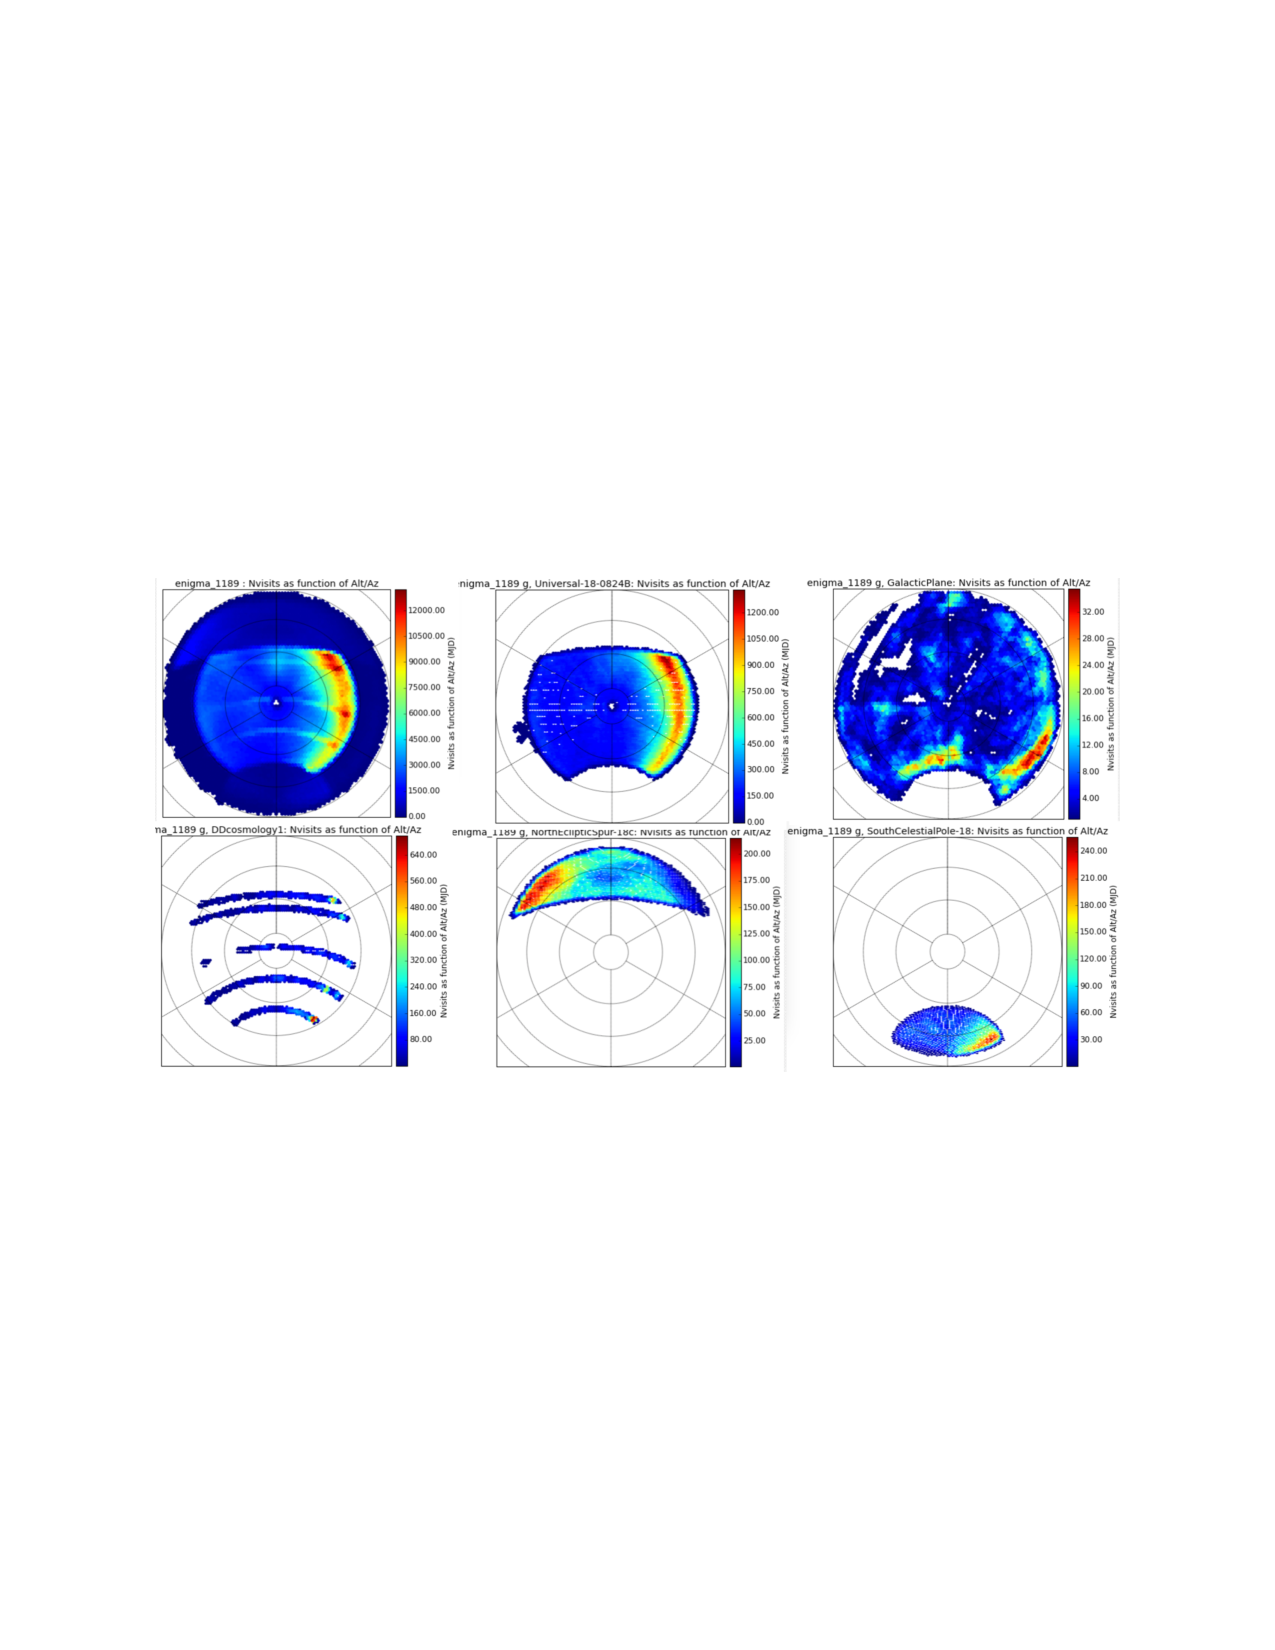
\includegraphics[angle=0,width=1.19\hsize:,clip]{figs/aaAllp.pdf}
\vskip -3.5in
\caption{The color-coded map in the top left panel shows the g band visit count from
Baseline Cadence simulation \opsimdbref{db:enigma} in the equal-area Lambert projection of the
horizontal coordinate system (altitude-azimuth), with north on top and west towards the
right. The horizon corresponds to the largest circle. Five implemented proposals are shown
separately in other panels (top row: Universal and Galactic Plane, bottom row: Deep Drilling
fields, North Ecliptic Spur, and South Celestial Pole region). The Universal cadence was
limited to airmass below 1.5, while other proposals sampled higher airmass, too (see the
histogram in \autoref{fig:airmassenigma}).  Note the strong propensity of Universal fields
for westward observations (the median airmass is about 1.2).}
\label{fig:AltAzenigma}
\end{figure}
%%%%%%%%%%%%%%%%%%%%%%%%%%%%%%%%%

%%%%%%%%%%%%%%%%%%%%%%%%%%%%%%%%%
\begin{figure}[b!]
\vskip -1.1in
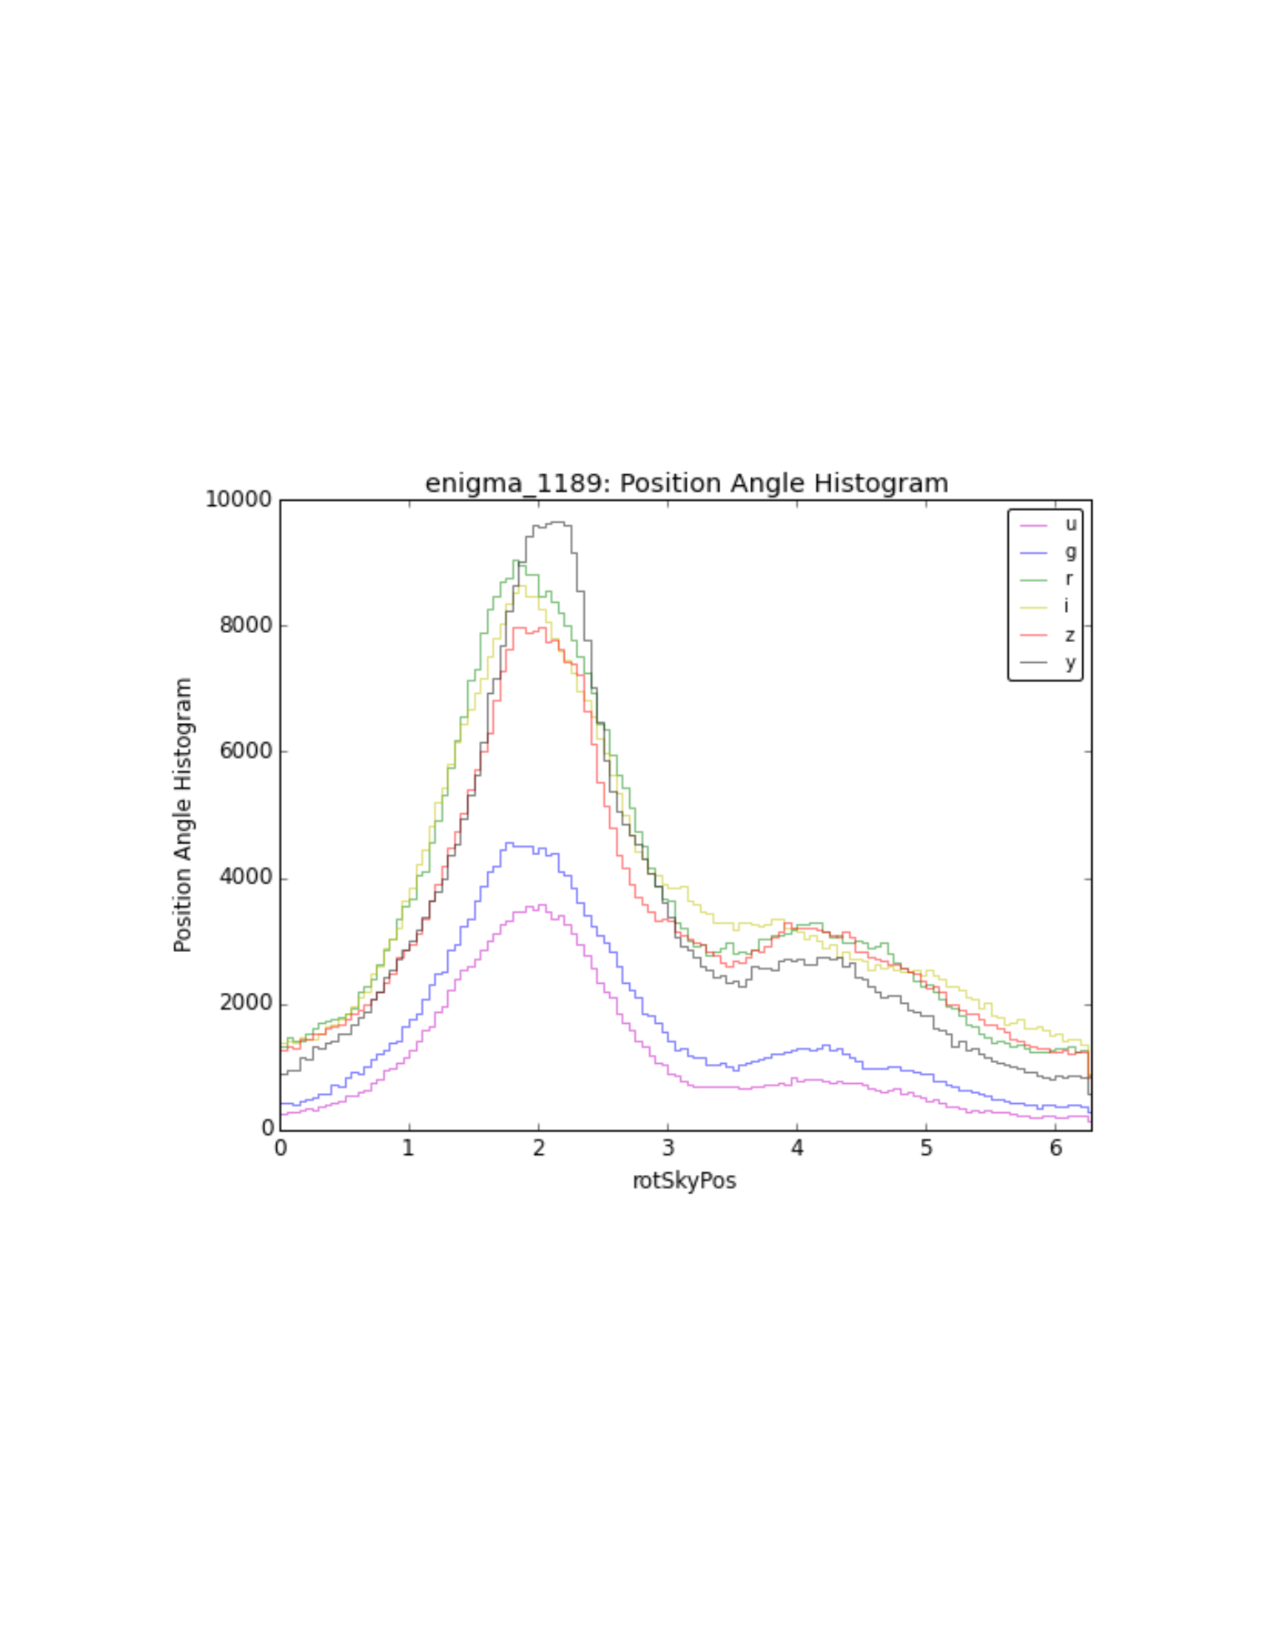
\includegraphics[angle=0,width=0.49\hsize:,clip]{figs/enigma1189_rotator.pdf}
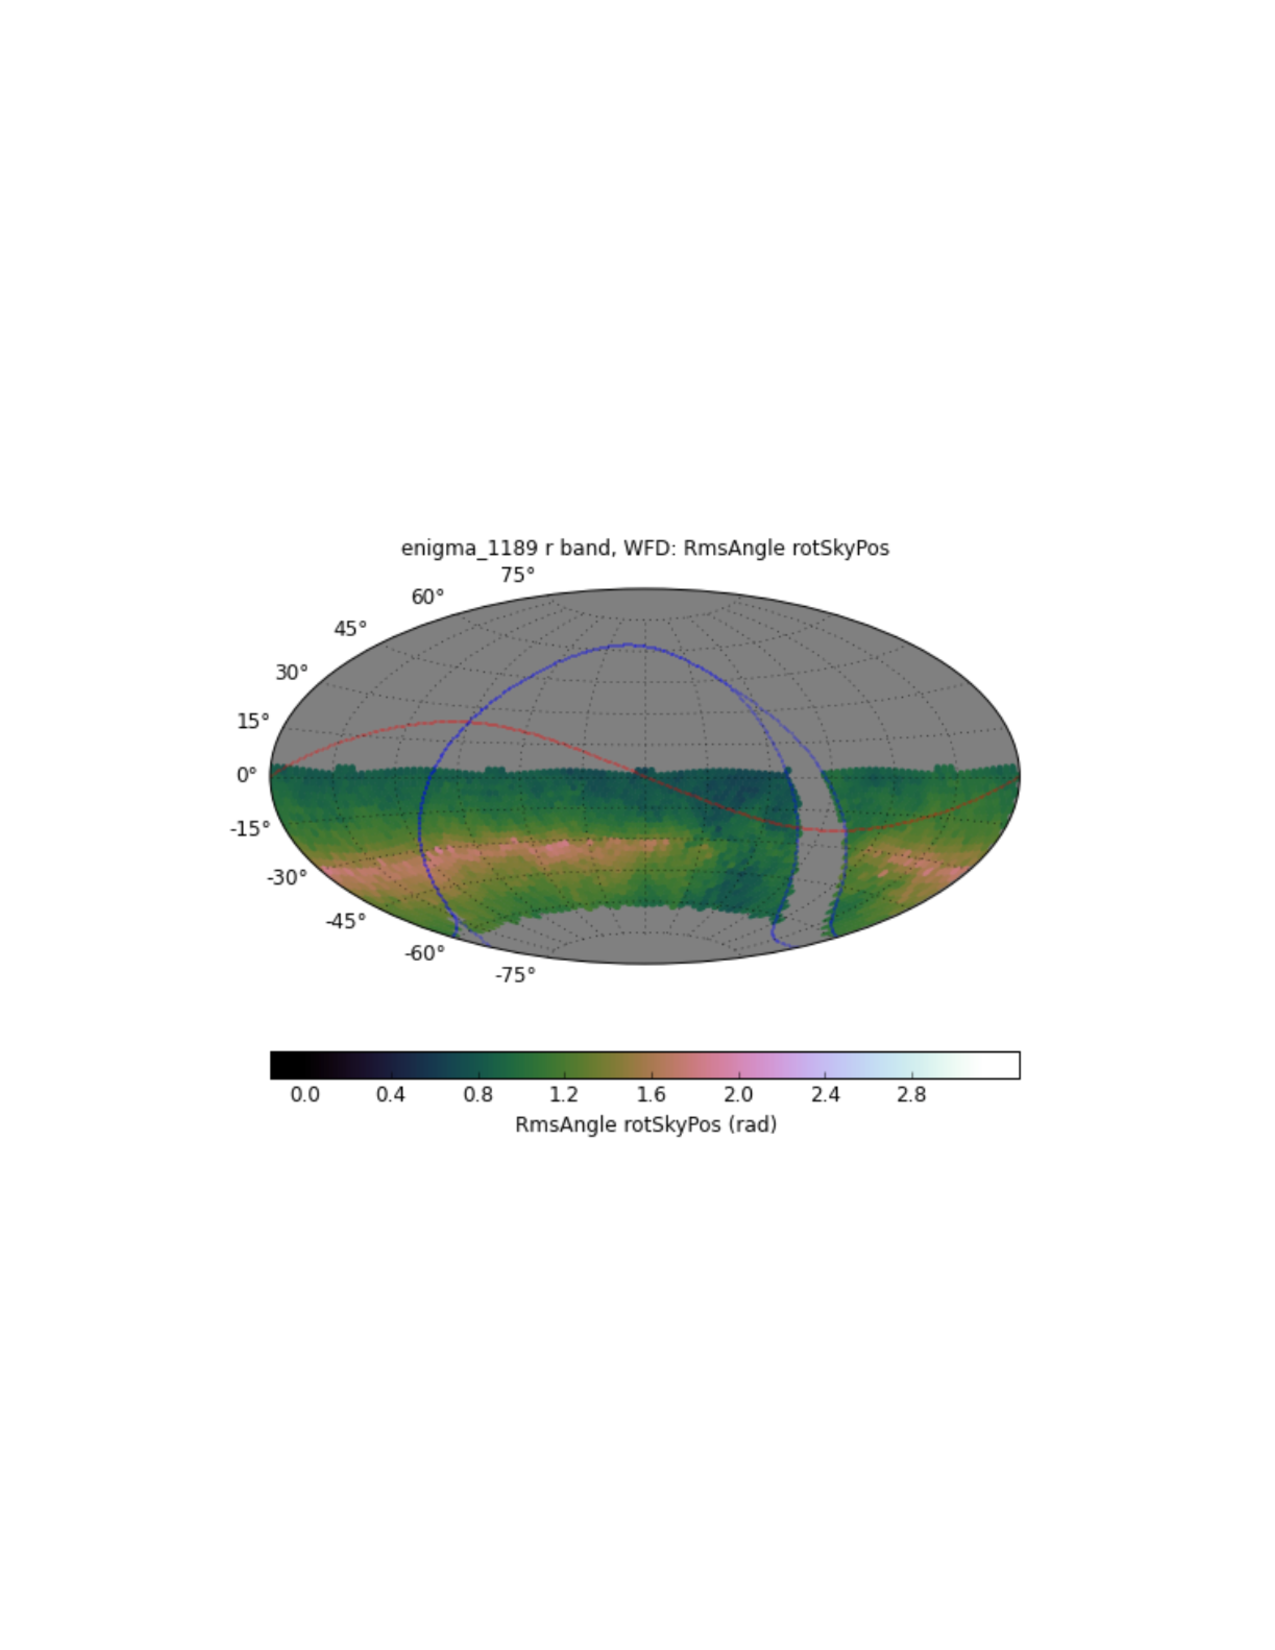
\includegraphics[angle=0,width=0.49\hsize:,clip]{figs/enigma1189_rotator2.pdf}
\vskip -1.3in
\caption{The left panel shows the position angle distribution (in radians)  in each band for the
main survey fields in \opsimdbref{db:enigma}. The position angle is the angle between ``up'' in the image
and North on the sky. The variation of the root-mean-square scatter of the $r$ band
distribution across the sky is shown in the right panel.}
\label{fig:rotator}
\end{figure}
%%%%%%%%%%%%%%%%%%%%%%%%%%%%%%%%%

%%%%%%%%%%%%%%%%%%%%%%%%%%%%%%%%%
\begin{figure}[t!]
\vskip -4.1in
\hskip -0.5in
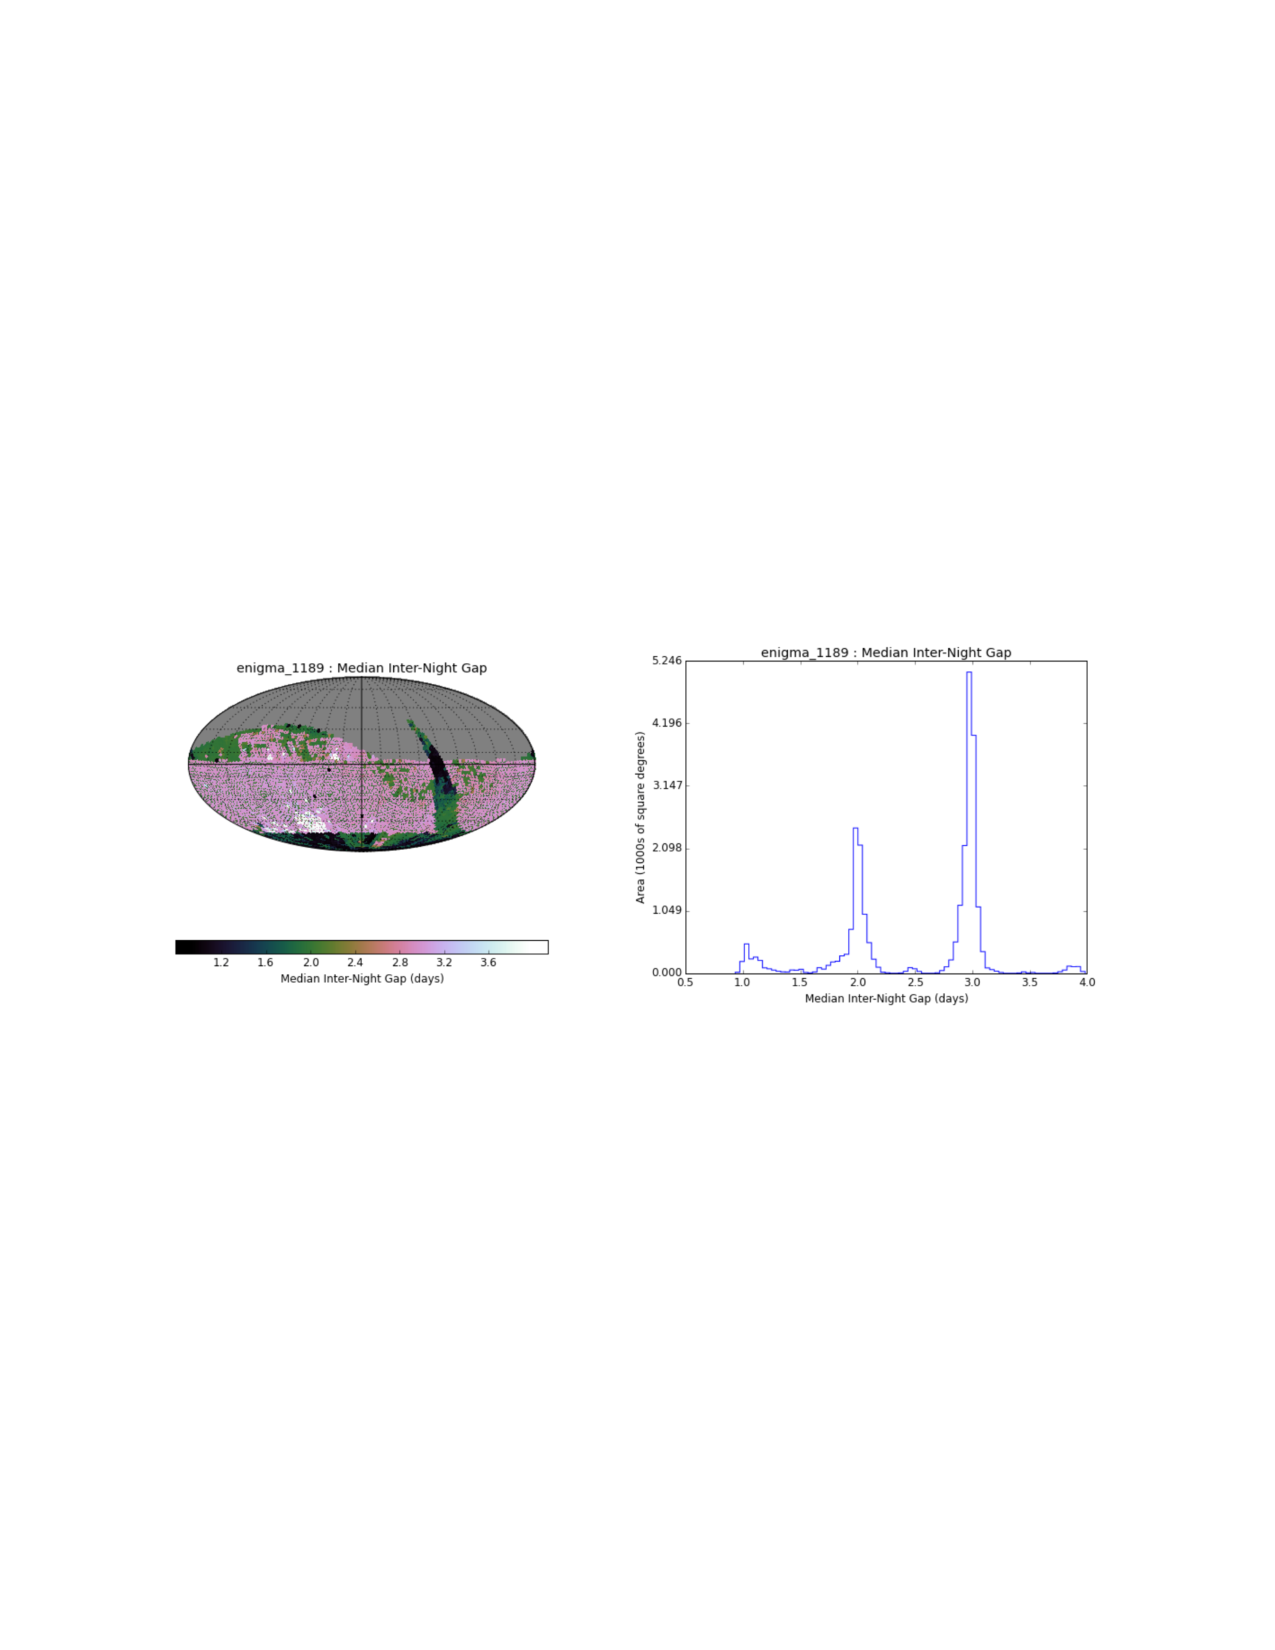
\includegraphics[angle=0,width=1.19\hsize:,clip]{figs/enigma1189_interGapAll.pdf}
\vskip -4.0in
\caption{The median inter-night gap (or revisit time) is shown in Aitoff projection
for all proposals and all filters for candidate Baseline Cadence \opsimdbref{db:enigma}.
On average, fields in the main survey get revisited about every 3 days.}
\label{fig:enigmaGapAll}
\end{figure}
%%%%%%%%%%%%%%%%%%%%%%%%%%%%%%%%%

%%%%%%%%%%%%%%%%%%%%%%%%%%%%%%%%%
\begin{figure}[h!]
\vskip -3.8in
\hskip -0.5in
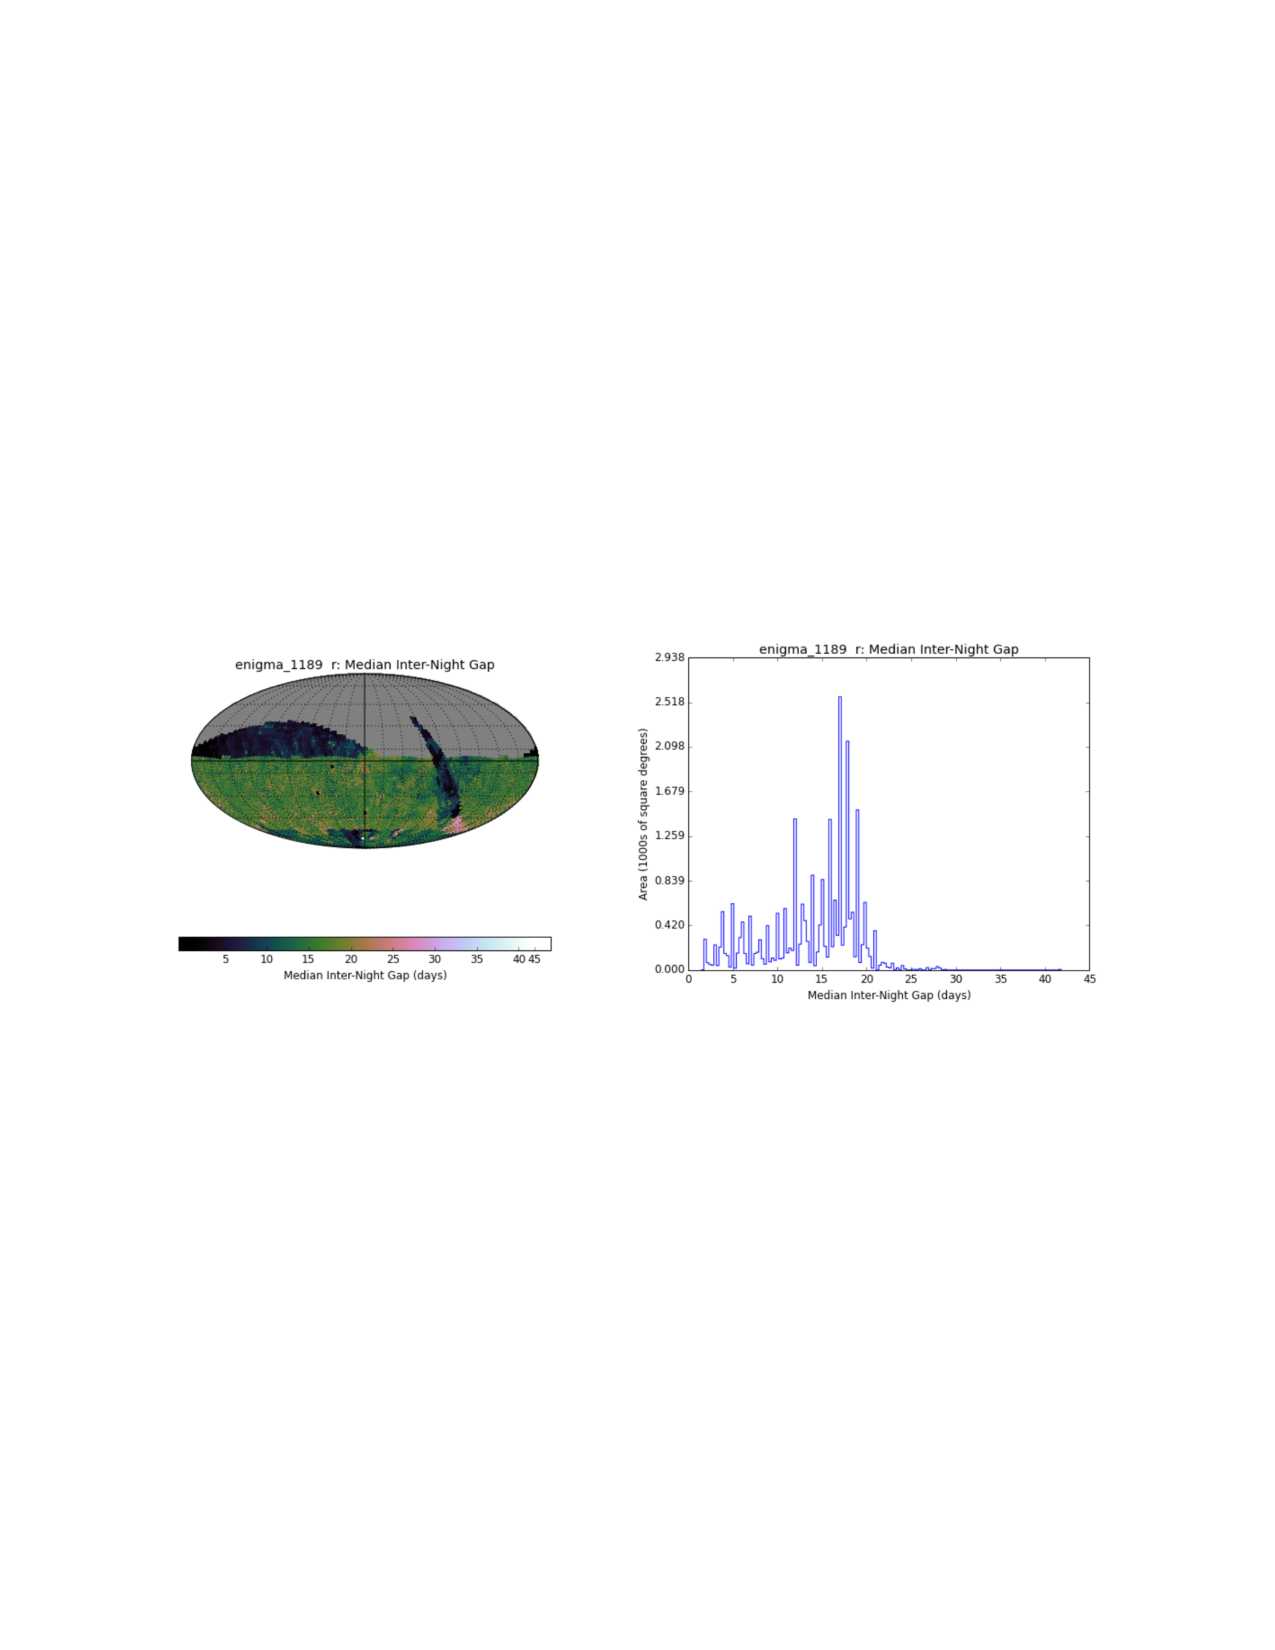
\includegraphics[angle=0,width=1.19\hsize:,clip]{figs/enigma1189_interGap_r.pdf}
\vskip -4.0in
\caption{The median inter-night gap for r band visits is shown in Aitoff projection
for all proposals and all filters for candidate Baseline Cadence \opsimdbref{db:enigma}.
On average, fields in the main survey get revisited in the r band about every 15 days.}
\label{fig:enigmaGapr}
\end{figure}
%%%%%%%%%%%%%%%%%%%%%%%%%%%%%%%%%

%%%%%%%%%%%%%%%%%%%%%%%%%%%%%%%%%
\begin{figure}[b!]
\vskip -3.8in
\hskip -0.5in
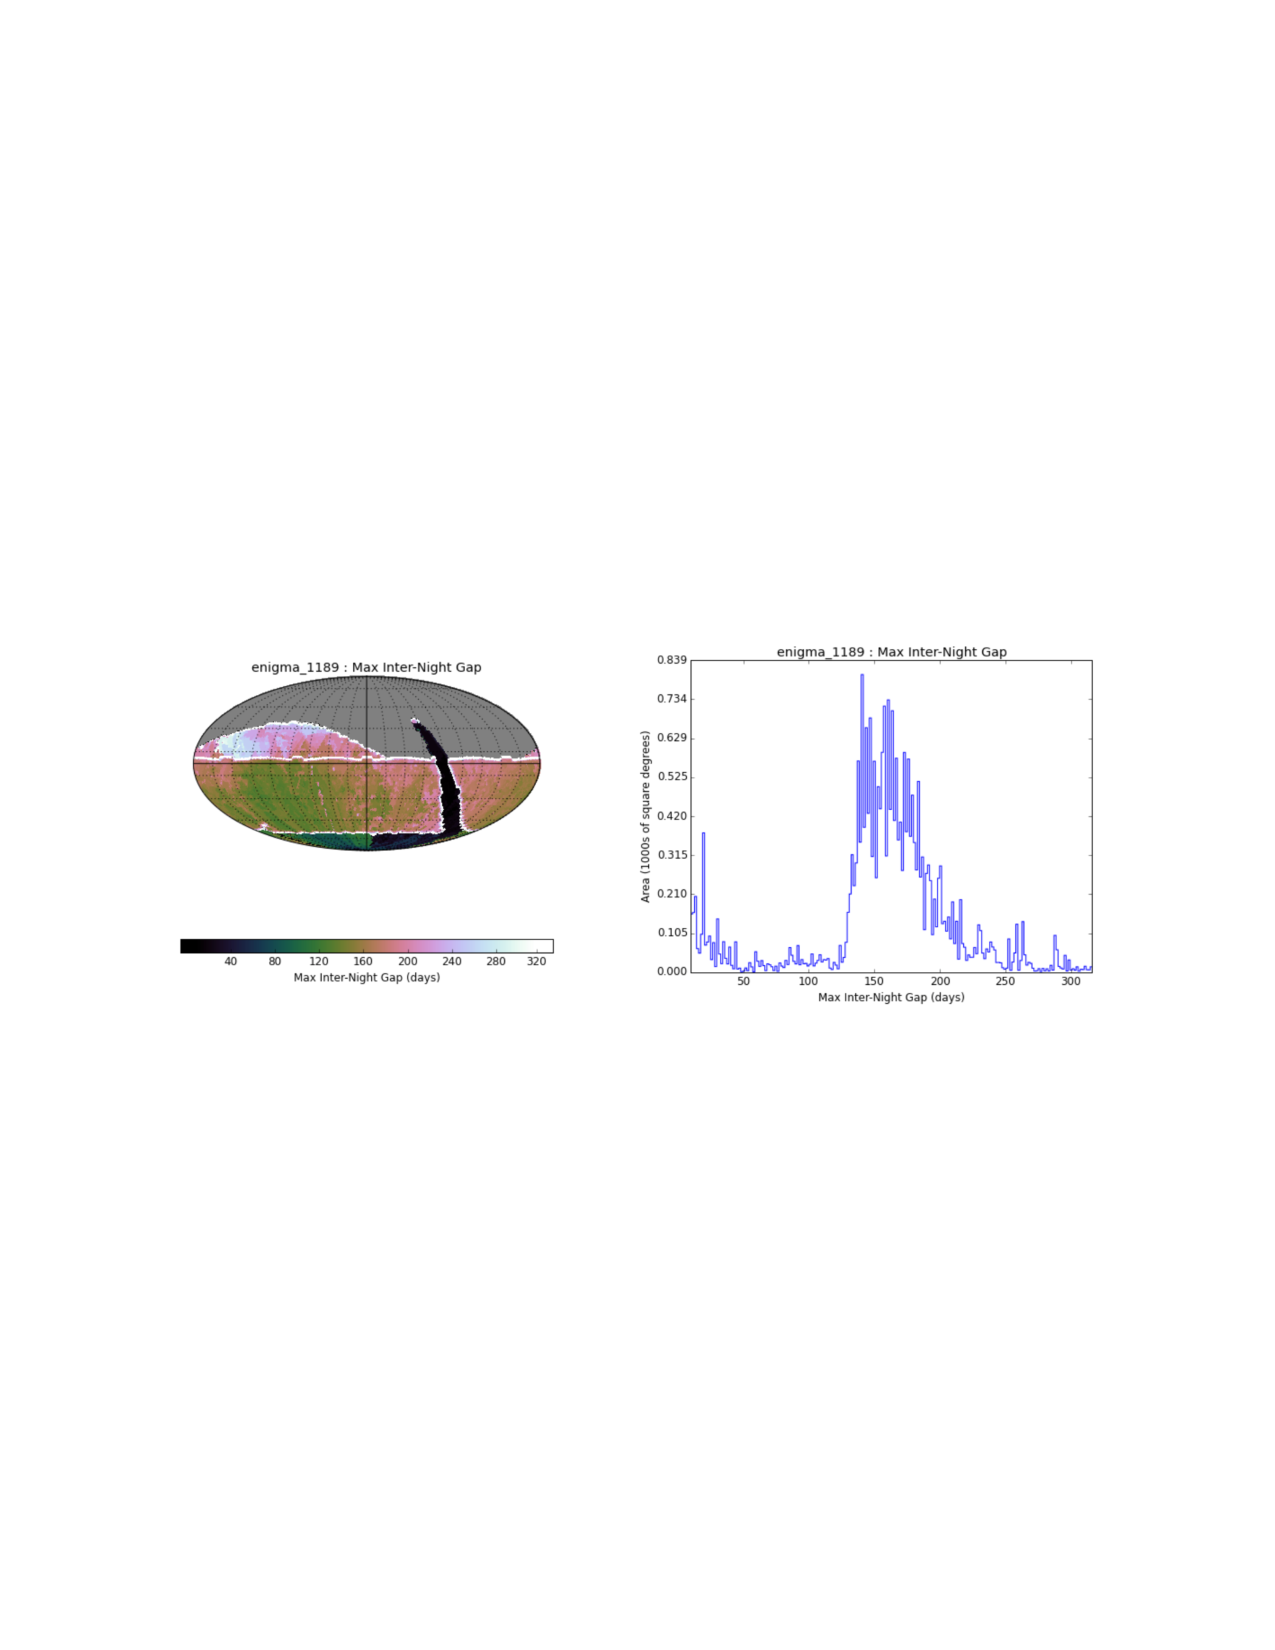
\includegraphics[angle=0,width=1.19\hsize:,clip]{figs/enigma1189_MAXinterGapAll.pdf}
\vskip -4.0in
\caption{The maximum inter-night gap (or revisit time) is shown in Aitoff projection
for all proposals and all filters for candidate Baseline Cadence \opsimdbref{db:enigma}.}
\label{fig:enigmaMAXGapAll}
\end{figure}
%%%%%%%%%%%%%%%%%%%%%%%%%%%%%%%%%

%%%%%%%%%%%%%%%%%%%%%%%%%%%%%%%%%
\begin{figure}[t!]
\vskip -4.1in
\hskip -0.5in
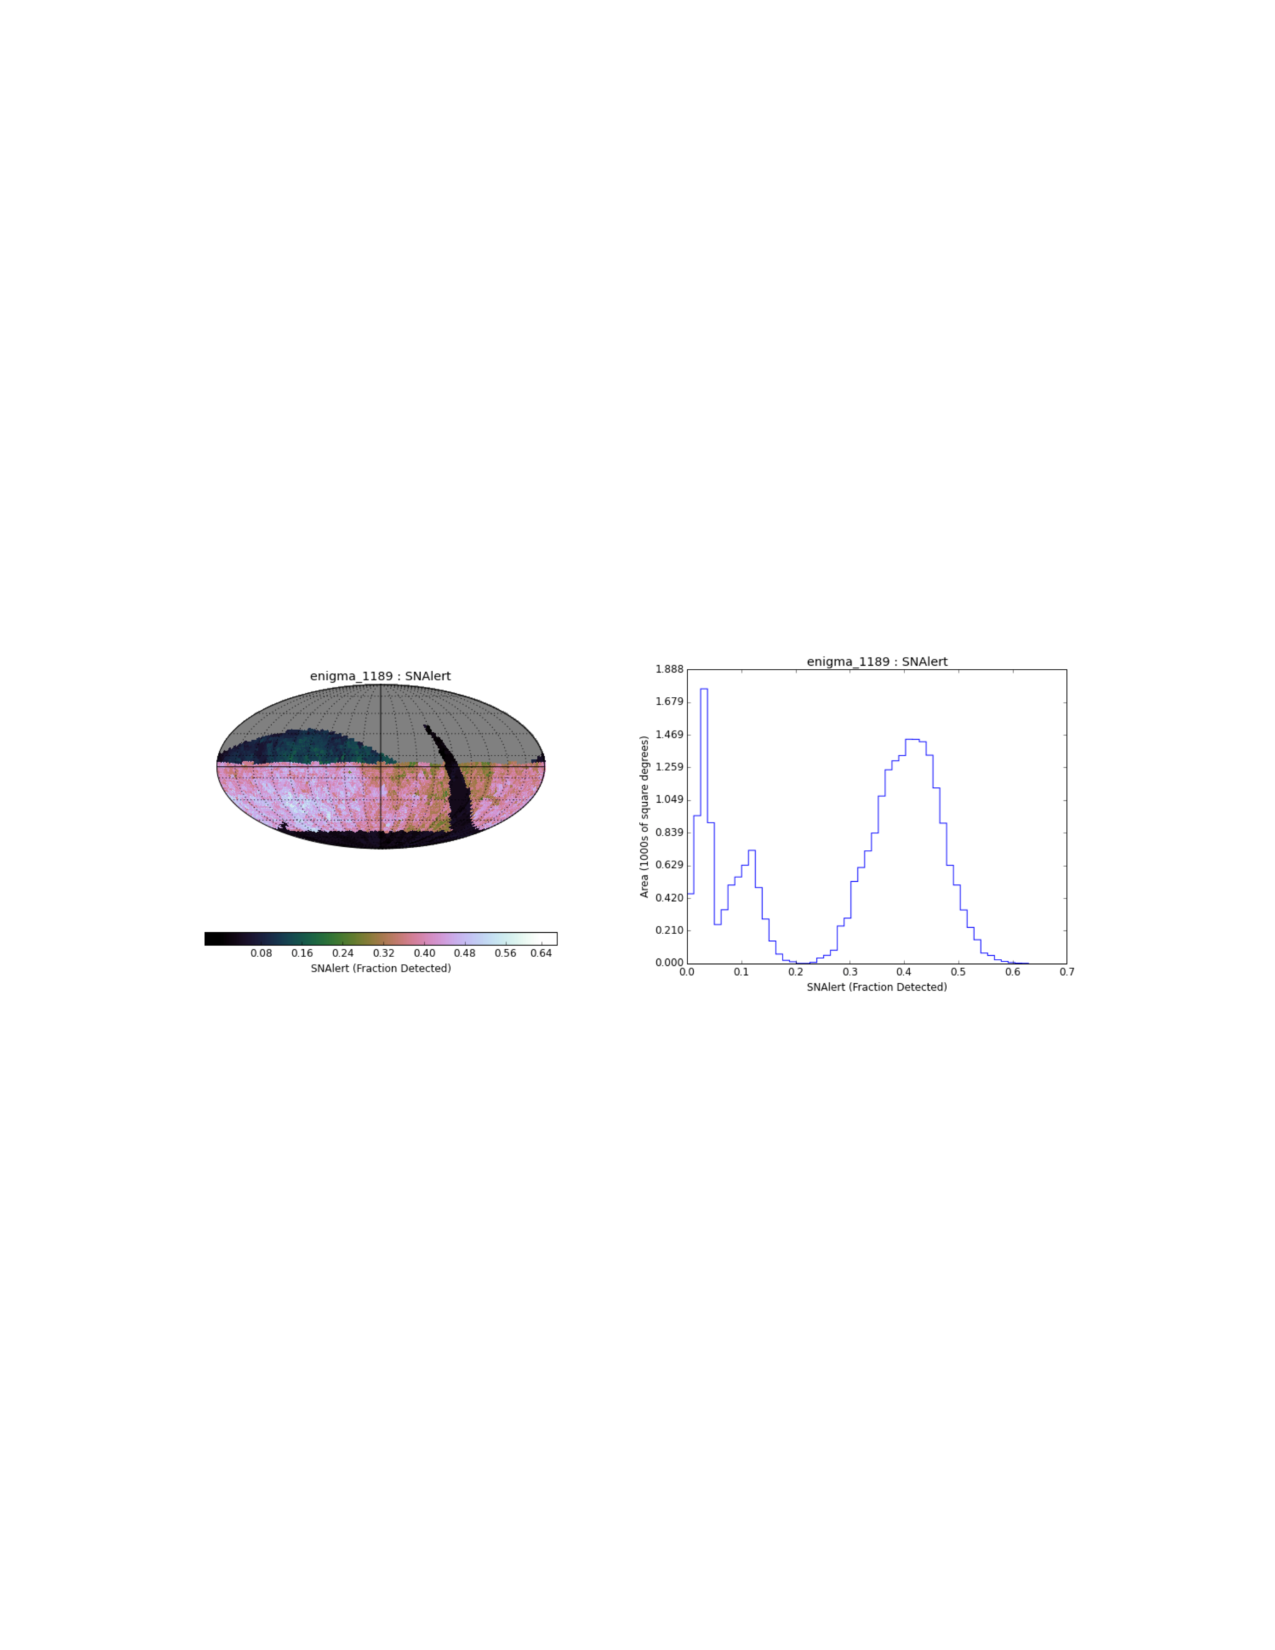
\includegraphics[angle=0,width=1.19\hsize:,clip]{figs/enigma1189_earlySNe.pdf}
\vskip -4.0in
\caption{The fraction of simulated Type Ia SNe at a redshift of 0.5 detected
pre-peak in any filter for candidate Baseline Cadence \opsimdbref{db:enigma}. About
40\% of all such SNe from the main survey will be detected before their
maximum brightness.}
\label{fig:enigmaEarlySNe}
\end{figure}
%%%%%%%%%%%%%%%%%%%%%%%%%%%%%%%%%


For comparison, the current Baseline Cadence, \texttt{opsim3.61}
(obtained with old OpSim code), delivered 2,651,588 visits, or 7.4\%
more than \opsimdbref{db:enigma}  (this is due to known effects and
changes in the code,  such as more pre-scheduled down time in the new
version). Perhaps the most important (and undesired!) difference
between the two simulations is that the new candidate Baseline Cadence
spent 6.4\% of the observing time on North Ecliptic Spur proposal (vs.
4\% spent on corresponding Universal North proposal in
\texttt{opsim3.61}), and less than 90\% of time on the Universal
proposal (the main wide-deep-fast survey).

Analysis of the hour angle distribution, shown in
\autoref{fig:HAenigma} and \autoref{fig:AltAzenigma}, reveals a strong
bias towards observations west from the meridian for the main survey.
{\it This pattern is not fully understood at this time} and may be
caused by specific features of the cost function implemented in the
OpSim code.

Another potentially undesireable feature, seen in practically all
simulations analyzed here, is that up to about a quarter of visits in
the main survey area represents the third, the fourth and sometimes
even the fifth visit to a field in the same night. For a large number
of time-domain programs, these visits could be used instead to
decrease the field inter-night revisit time. For more details, see
\autoref{sec:cadexp:NEOs}. The position angle distributions for this simulation
are shown in \autoref{fig:rotator}.


\subsubsection{Time-domain metrics}

The analysis of metrics designed for time-domain science has not been
performed yet in detail, except for the analysis of asteroid
completeness discussed in \autoref{sec:cadexp:NEOs}. MAF already includes
several sophisticated metrics, e.g., period recovery for variable
stars, which will be described in a later version of this report.

As a brief illustration of time-domain analysis,
\autoref{fig:enigmaGapAll} shows the median revisit time distribution
when all bands are considered, and \autoref{fig:enigmaGapr} shows the
median revisit time distribution in the band.  On average, fields in
the main survey get revisited about every 3 days using all filters,
and every 15 days when using only r band visits (30 days when using
only u band visits is the longest median revisit time).
\autoref{fig:enigmaMAXGapAll} shows the maximum inter-night gap, which
on average is about 5-6 months.

The temporal sampling for this simulation is sufficient to enable a
large recovery fraction for SNe. \autoref{fig:enigmaEarlySNe} shows
that a large fraction of LSST SNe will be detected before their
maximum brightness. Similar MAF metrics that explore various quality
cuts on SNe light curves (e.g. ``detected at least 6 times, at least 3
pre-peak, at least 3 post-peak, with observations in at least 3
filters'').

Intra-night revisit time distribution is discussed in more detail in
\S\ref{sec:cadexp:NEOs}.


\subsubsection{Special Proposals}

Regarding the special proposals, here we only provide the basic
performance parameters. With the exception of the Deep Drilling
proposal, these proposals are essentially strawman placeholders. The
North Ecliptic proposal (6.4\% of the observing time) obtained an
additional 300 visits per field, summed over $griz$ bands. These
fields are placed along the northern part of the Ecliptic. The
Galactic plane proposal (1.7\%) obtained 30 visits per band in all six
bands, across the region extending in Galactic latitude 10 degrees
from the Galactic center, with the boundary approaching the Galactic
equator linearly with longitude, and the zone ending at $l=90$ deg.
and at $l=270$ deg. The South Celestial pole proposal (2.1\%) obtained
30 visits per band in all six bands, for fields centers with Dec $<
-62.5$ deg. The Deep Drilling cosmology proposal (4.5\%) included 5
fields, with each obtaining several thousand visits per band. The
coadded $5\sigma$ depths for these fields are much fainter than for
the main survey: the medians values are (28.5, 28.6, 28.8, 28.2, 27.7,
26.0) in the $ugrizy$ bands, respectively.


\vskip 0.2in
{\bf Conclusions:}

The candidate “Baseline Cadence”, \opsimdbref{db:enigma}, appears to
be an adequate replacement for the current baseline cadence
(\texttt{opsim3.61}). Based on this preliminary analysis, there are no
major problems with its performance. While there are patterns which
are not fully understood (most notably the observing bias towards
west),  or undesired (unnecessary revisits of the same field in the
same night), \opsimdbref{db:enigma} is used as a benchmark cadence,
and referred to as ``Baseline Cadence'',  in the rest of this
document\footnote{Assuming that additional analysis will not uncover
any major deficiencies, this simulation will be discussed by the
Project Science Team and proposed for adoption as the new Baseline
Cadence to the Change Control Board. The target date for this proposal
is late September 2015.}

An important feature of \opsimdbref{db:enigma} simulation is that the
mean slew time of 6.9 sec is very close to the minimum possible slew
time of about 4.5 sec. The implication is that the surveying
efficiency, assuming 30 sec exposure time per visit, can be increased
by at most about 6\% (that is, the total open-shutter time is within
about 6\% from its possible maximum, given everything else unchanged).
Nevertheless, there are other survey aspects, including sky coverage
and temporal sampling functions, that can be further optimized, as
discussed in \autoref{sec:CE}.

\navigationbar

% --------------------------------------------------------------------

\section{Some Simulated Alternative Observing Strategies}
\def\secname{cadexp:alternatives}\label{sec:\secname}

We now describe some alternatives to the Baseline Cadence that were
explored. These \OpSim databases are all available for further testing
with science-based MAF metrics.

% - - - - - - - - - - - - - - - - - - - - - - - - - - - - - - - - - -

%%%%%%%%%%%%%%%%%%%%%%%%%%%%%%%
\opsimdb[db:opstwo]{ops2\_1098}{Only Universal Cadence, with pairs of visits.}
%%%%%%%%%%%%%%%%%%%%%%%%%%%%%%%

{\bf Motivation and description:} Formally, $\sim$90\% of observing
time is allocated to the main Universal Cadence program (WFD). The
remaining observing time is allocated to other programs, such as
``Deep Drilling'' programs (see Section 3.4 and Tables 22-26  in the
SRD). With this simulation, we wished to find out what would be the
effect of ignoring special programs and spending all of the observing
time on the main Universal Cadence program. \\

{\bf Expectations:} About 2.11 million visits (85\% of 2.47 million
visits) from Baseline Cadence (\opsimdbref{db:enigma}) were allocated
to WFD cadence. Here we expect that all of these 2.47 million visits
will be allocated to WFD cadence. \\

{\bf Analysis Results:} This simulated cadence is named \opsimdbref{db:opstwo}.
Compared to the Baseline Cadence \opsimdbref{db:enigma}:
\begin{enumerate}
\item The total number of visits is close to the expected value: 2.45 million.
The minimum number of visits per field for the 2,293 WFD fields in Baseline Cadence
is 968 for this simulation, compared to 898 for Baseline Cadence.
\item The median number of visits per night and the mean slew time are
essentially the same as for Baseline Cadence (810 vs. 815 and 7.2 sec vs. 6.9 sec).
\item The median seeing, sky brightness and airmass in the r and i bands are
      essentially the same as for WFD fields in Baseline Cadence.
\item The median trigonometric parallax and proper motion errors are improved by
about 8\%, with improvements commensurate with the increase in the number of visits.
\item This simulation also shows observing bias towards west (that is, additional
special programs in \opsimdbref{db:enigma} are not reponsible for this bias).
\end{enumerate}


{\bf Conclusions:} \opsimdbref{db:opstwo}, using only uniform cadence
proposal, delivered 99.2\% of the number of visits obtained by
Baseline Cadence. Therefore, {\it the ``filler'' aspect of other
proposals does not have a major impact on the surveying efficiency}.
The minimum number of visits per field for the 2,293 WFD fields in
Baseline Cadence is 968 (the SRD design value is 825 and the stretch
goal value is 1000). Although the sky coverage of these 2293 fields is
about 18,000 sq.deg., their cumulative area is 22,000 sq.deg. With
proper dithering, the effective number of visits could be increased to
968*22/18 = 1183 (or the WFD area increased from 18,000 sq. deg.; see
analysis of ops2\_1092 below). This increase is an improvement of 43\%
relative to the SRD design specification of 825 visits over 18,000
sq.deg. However, note again that there are no other programs in this
simulation (i.e., if other programs were allocated 10\% of the
observing time, the implied overall ``over-performance'' in the number
of  visits would be about 30\%).

% - - - - - - - - - - - - - - - - - - - - - - - - - - - - - - - - - -

%%%%%%%%%%%%%%%%%%%%%%%%%%%%%%%%%
\opsimdb[opstwoPS]{ops2\_1092}{A Pan-STARRS-like observing strategy.}
%%%%%%%%%%%%%%%%%%%%%%%%%%%%%%%%%

{\bf Motivation and description:} "Pan-STARRS-like cadence” attempts
to apply a uniform cadence strategy throughout the survey region,
which is maximized and defined by Dec $< +15$ deg (about 27,400
deg$^2$). The maximum acceptable airmass is kept at its default value
of 1.5 (which excludes fields with Dec $< -78$ deg and Dec $> +18$
deg. This simulation utilizes uniform cadence and no other proposal,
and requires pairs of visits as in Baseline Cadence. \\

{\bf Expectations:} The total number of visits should be roughly the
same as in Baseline Cadence, but spread over a 42\% larger sky area
(3,255 fields instead of 2,293), with fewer visits per field. \\

{\bf Analysis Results:}  This simulated cadence is named \opsimdbref{db:opstwoPS}.
Compared to the Baseline Cadence \opsimdbref{db:enigma}:
\begin{enumerate}
\item The total number of visits is 2.47 million, and essentially identical to the
number of visits in Baseline cadence.
\item
The mean number of visits per field is 758.5, which is 98\% of the number of visits
for WFD fields obtained by Baseline Cadence (but here the sky area is 42\% larger).
\item The median number of visits per night and the mean slew time are
essentially the same as for Baseline Cadence.
\item The median seeing, sky brightnes and airmass in the r and i bands for WFD fields are
         essentially the same as in Baseline Cadence.
\item The median trigonometric parallax and proper motion errors show
uniform behavior over the entire enlarged area (see \autoref{fig:parapmenigma2}),
with the values similar to those obtained for Baseline Cadence.
\item This simulation also shows observing bias towards west.
\end{enumerate}

Due to increased sky area, which samples regions that can never
achieve low airmass, the median coadded depth is about 0.15 mag
shallower for this simulation than for Baseline Cadence. As a result,
the counts of galaxies per unit area down to a fixed SNR would
decrease by about 15-20\%. At the same time, the area outside the
Galactic plane is increased by about 30\%, and thus the total number
of galaxies would be increased by about 10\%, compared to WFD fields
in Baseline Cadence. However, the increased median airmass also
results in larger seeing, especially for the borderline regions, as
illustrated in \autoref{fig:PS-seeing}. The increased median seeing
would decrease the number of galaxies effectively resolved for weak
lensing by about 3-5\%. In addition, the additional area has somewhat
larger extinction due to interstellar dust which further decreases the
galaxy counts (this impact of dust extinction is not yet implemented
in MAF). As a result of these effects, the two strategies result in
similar weak lensing galaxy samples.

{\bf Conclusions:} When only the Universal Cadence proposal is
employed, the survey area could be increased by about 40\%, while
still delivering the mean number of fields at the level of 98\% of
that in Baseline Cadence (or 92\% of the SRD design value of 825).
Hence, simulations ops2\_1092  and \opsimdbref{db:opstwo} demonstrate
that the ``survey reserve'', relative to the Universal Cadence design
specifications from the SRD, can be used to i) increase the number of
visits per field over the WFD area,  or ii) increase the surveyed area
while keeping the number of visits per field statistically unchanged,
or iii) increase both area and the number of visits, and/or iv)
execute additional programs (the current baseline).


%%%%%%%%%%%%%%%%%%%%%%%%%%%%%%%%%
\begin{figure}[t!]
\vskip -0.03in
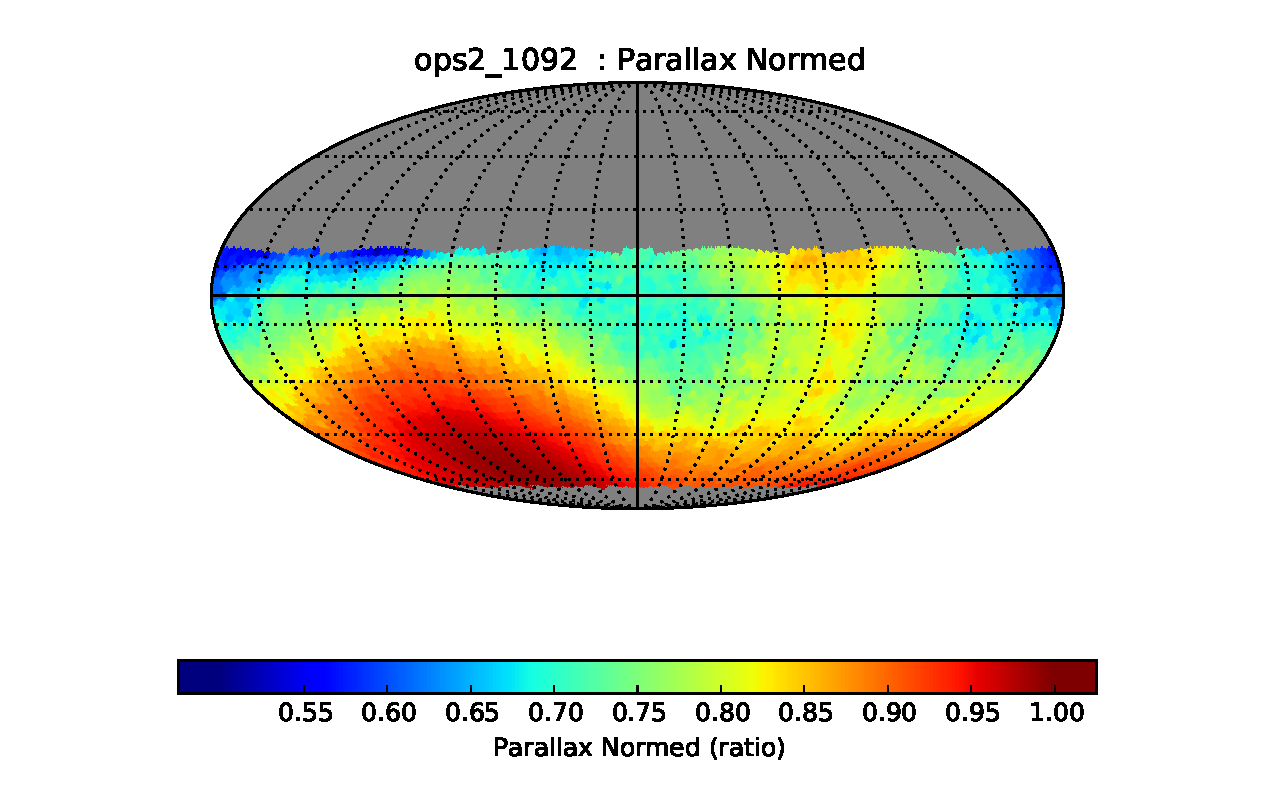
\includegraphics[angle=0,width=0.49\hsize:,clip]{figs/ops2_1092_Parallax_Normed__HEAL_SkyMap.pdf}
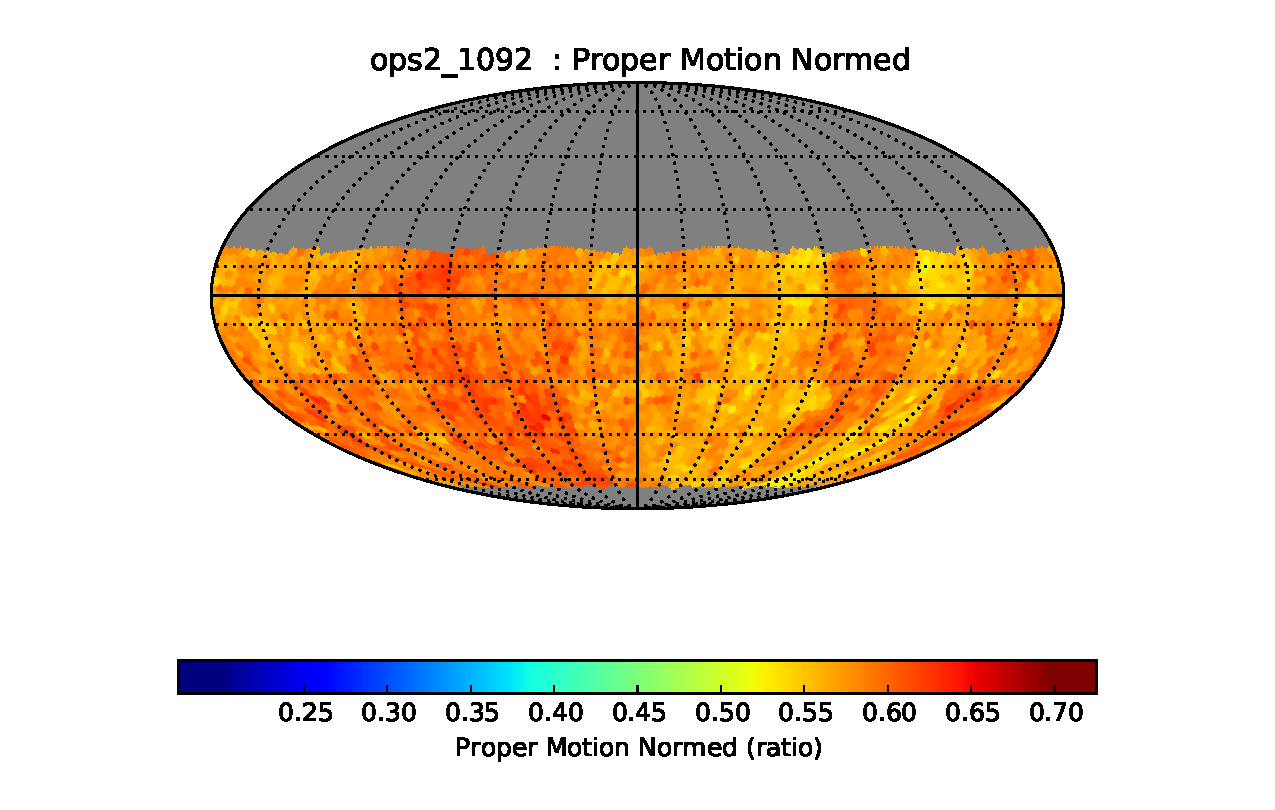
\includegraphics[angle=0,width=0.49\hsize:,clip]{figs/ops2_1092_Proper_Motion_Normed__HEAL_SkyMap.pdf}
\vskip -0.2in
\caption{The trigonometric parallax errors (left) and proper motion errors (right)  for simulated cadence
ops2\_1092 (``Pan-STARRS-like'' cadence), normalized by the values for idealized perfectly optimized
cadence, are shown in Aitoff projection of equatorial coordinates (compare to \autoref{fig:parapmenigma}).}
\label{fig:parapmenigma2}
\end{figure}
%%%%%%%%%%%%%%%%%%%%%%%%%%%%%%%%%

%%%%%%%%%%%%%%%%%%%%%%%%%%%%%%%%%
\begin{figure}[t!]
\vskip -3.9in
\hskip -0.5in
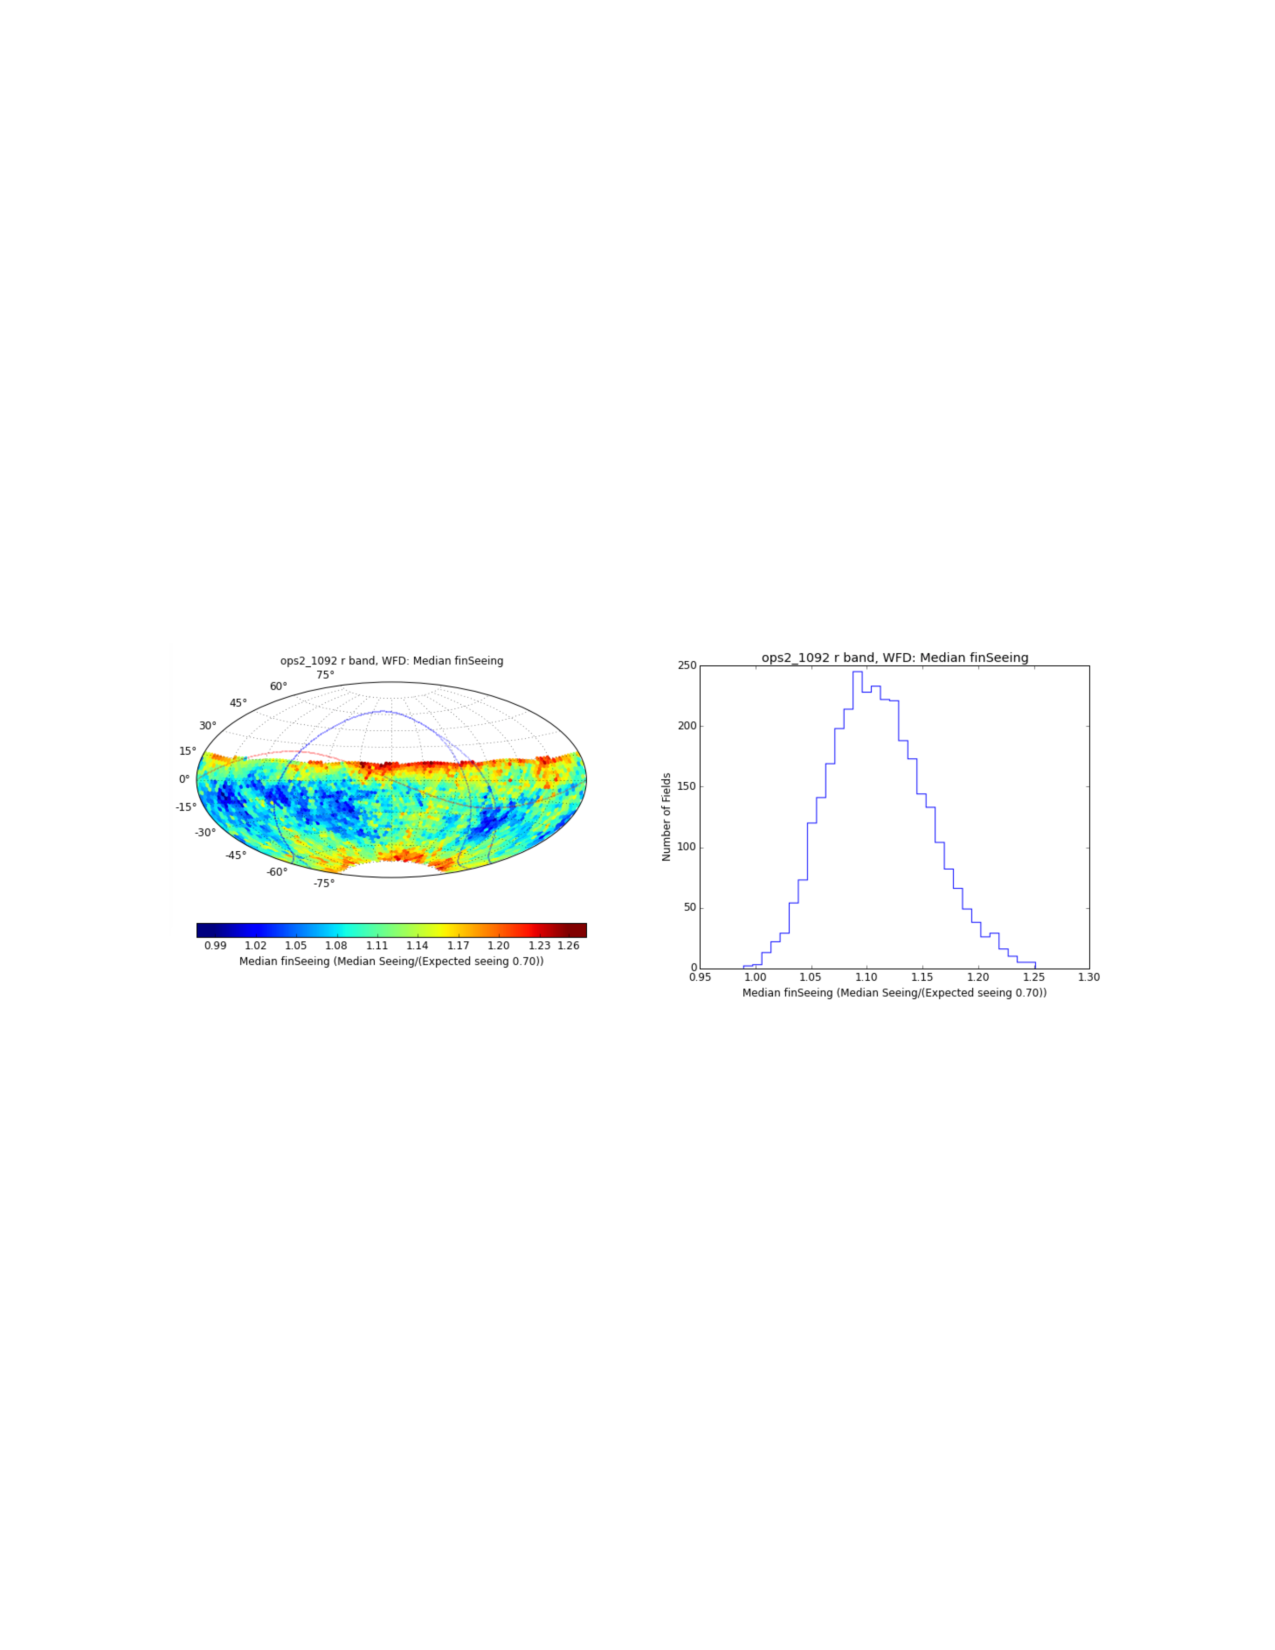
\includegraphics[angle=0,width=1.19\hsize:,clip]{figs/PS-seeing.pdf}
\vskip -4.0in
\caption{The median seeing in r filter, for simulated cadence ops2\_1092 (``Pan-STARRS-like'' cadence),
normalized by expected value (0.70). Note that fields with the most positive and most negative
declination have on average larger values. For comparison, the median normalized seeing for WFD fields
in Baseline Cadence is 1.08, with a negligible fraction of fields with values above 1.18.}
\label{fig:PS-seeing}
\end{figure}
%%%%%%%%%%%%%%%%%%%%%%%%%%%%%%%%%


% - - - - - - - - - - - - - - - - - - - - - - - - - - - - - - - - - -

%%%%%%%%%%%%%%%%%%%%%%%%%%%%%%%%%%%%%%%%%%%
\opsimdb[db:UConlyNoVisitPairs]{ops2\_1093}{Only Universal Cadence, no visit pairs.}
%%%%%%%%%%%%%%%%%%%%%%%%%%%%%%%%%%%%%%%%%%%

{\bf Motivation and description:} The main goal of this simulation was
to assess the impact of the requirement for visit pairs on the survey
efficiency (Baseline Cadence requests two visits per night to the same
field, separated in time by about an hour, and driven by asteroid
orbit determination). It is plausible that the removal of this
requirement could result in a more efficient survey. In order to allow
as simple analysis as possible, only the Universal Cadence proposal is
requested. Hence, this simulation should be directly compared to
simulation \opsimdbref{db:opstwo}. \\

{\bf Expectations:} If the requirement for visit pairs decreases
surveying efficiency, then this simulation should deliver more than
2.45 million visits delivered by \opsimdbref{db:opstwo}. \\

{\bf Analysis Results:} This simulated cadence is named \opsimdbref{db:UConlyNoVisitPairs}. Compared
to \opsimdbref{db:opstwo}:
\begin{enumerate}
\item The total number of visits is 2.45 million, identical to \opsimdbref{db:opstwo}.
\item The median slew time, and the median coadded depth and seeing in the $r$ band
are essentially identical, too.
\item The median airmass in the $r$ band of 1.26 is a bit higher than 1.20 obtained
for \opsimdbref{db:opstwo}.
\item The median fraction of revisits faster than 30 minutes of 0.35 is smaller than 0.39
for \opsimdbref{db:opstwo}, and is consistent with the absence of pair contributions (that is,
such revisits are due to field edge overlaps, and unintentional revisits, in case of \opsimdbref{db:UConlyNoVisitPairs}).
\end{enumerate}

{\bf Conclusions:} The comparison of this simulation and
\opsimdbref{db:opstwo} shows that requiring pairs of visits (in a
given observing night) does not result in an appreciable loss of
surveying efficiency. Indeed, pairs of visits result in a better
short-timescale coverage that would enhance many types of time-domain
science (and, of course, it's crucial for asteroid science).


% - - - - - - - - - - - - - - - - - - - - - - - - - - - - - - - - - -

%%%%%%%%%%%%%%%%%%%%%%%%%%%%%%%%%%%%%%%%%%%
\opsimdb[db:NoVisitPairs]{kraken\_1032}{Baseline Cadence, but with no visit pairs.}
%%%%%%%%%%%%%%%%%%%%%%%%%%%%%%%%%%%%%%%%%%%

{\bf Motivation and description:} The main goal of this simulation was
to assess the impact of the requirement for visit pairs on the survey
efficiency. Instead of the idealized case above which compared only
the Universal Cadence proposal fields, in this more realistic case
{\it all proposals from Baseline Cadence are executed}. Hence, this
simulation should be compared to Baseline Cadence
(\opsimdbref{db:enigma}). \\

{\bf Expectations:} A slight, or no, increase in surveying efficiency
and thus the total number of visits is expected when compared to
Baseline Cadence. \\

{\bf Analysis Results:}  This simulated cadence is named
\opsimdbref{db:NoVisitPairs}. Compared to \opsimdbref{db:enigma},
\begin{enumerate}
\item The total number of visits is 2.53 million, or 2.4\% more than
in Baseline Cadence.
\item The mean slew time is 5.8 sec, or 16\% shorter than for Baseline
Cadence. This decrease in the mean slew time implies an efficiency
increase of 2.8\% and explains the actual 2.4\% improvement implied by
the total number of visits.  Note that this simulation has the
shortest mean slew time of all simulations investigated here (the
nominal shortest slew and settle time is about 4.5 sec).
\item The median airmass in the r band is slightly larger for this
simulation than for Baseline Cadence: 1.29 vs. 1.23.
\end{enumerate}


{\bf Conclusions:}
Unlike the comparison of \opsimdbref{db:UConlyNoVisitPairs} and
\opsimdbref{db:opstwo}, here the removal of visit pair requirement
results in a 16\% shorter mean slew time and consequently in 2.4\%
more visits.

% - - - - - - - - - - - - - - - - - - - - - - - - - - - - - - - - - -

%%%%%%%%%%%%%%%%%%%%%%%%%%%%%%%%%%%%%%%%%%%
\opsimdb[db:ShortExptime]{ops1\_1163}{Baseline Cadence, but with 33\% shorter exposure time.}
%%%%%%%%%%%%%%%%%%%%%%%%%%%%%%%%%%%%%%%%%%%

{\bf Motivation and description:} The optimal exposure time per visit
for the main survey, in the limit of a single value for all bands and
at all times, is in the range of about 20--60 seconds (see Section
2.2.2 in the LSST overview paper, arXiv:0805.2366, version 3.1). This
simulation investigates the effect of decreasing the exposure time per
visit to 20 seconds (from its nominal value of 30 seconds). The
shorter exposure time results in 0.22 mag shallower faint limit per
visit (the effect is larger in the $u$-band, see
\opsimdbref{db:DoubleUbandExptime}). \\

{\bf Expectations:} The total number of visits is expected to increase
by about 50\%, compared to \opsimdbref{db:enigma}, to 3.70 million,
for the same survey efficiency. However, the shorter exposure time
will have a significant impact on the survey efficiency: assuming a
slew time of 7 sec, the efficiency drops from 73\% to 65\% (comparing
30/(30+4+7) vs. 20/(20+4+7)). Therefore, the expected increase in the
number of visits is about 32\% and the expected number of visits is
3.2 million.  \\

{\bf Analysis Results:}  This simulated cadence is named
\opsimdbref{db:ShortExptime}. Compared to Baseline Cadence:
\begin{enumerate}
\item The total number of visits is 3.29 million, representing an
increase of 33\% that is very close to the expected value of 32\%.
\item The median number of visits per night is 1091, or about 34\%
more than for Baseline Cadence. The total open shutter time is 11\%
smaller for this simulation, and easily understood as due to expected
11\% decrease due to smaller surveying efficiency (the mean slew time
is practically the same as in Baseline Cadence, 6.8 sec vs. 6.9 sec).
\item The main survey (WFD, 18,000 sq. deg.) fields received 32\% more
visits than in Baseline Cadence. The increase in the minimum number of
visits over that area is 7\% (from 898 to 961). In addition, another
1,000 sq. deg. (6\% of the nominal WFD) area has more than 961 visits.
\item Most other performance parameters are essentially unchanged: the
fraction of visits spent on the main survey (84\% vs. 85\%), the
median seeing in the r band (0.78 arcsec vs. 0.77 arcsec), and the
median airmass (1.24 vs. 1.23).
\end{enumerate}

{\bf Conclusions:}
The comparison of \opsimdbref{db:ShortExptime} and
\opsimdbref{db:enigma} simulations demonstrates that the effect of
shorter exposures can be easily understood using simple efficiency
estimates. With the visit exposure time is decreased from 30 sec to 20
sec, the surveying efficiency and the total open shutter time drops by
$\sim$10\%, while the number of (shorter exposure time) visits (for
all proposals) increases by 33\%.



% - - - - - - - - - - - - - - - - - - - - - - - - - - - - - - - - - -

%%%%%%%%%%%%%%%%%%%%%%%%%%%%%%%%%%%%%%%%%%%
\opsimdb[db:LongExptime]{ops1\_1164}{Baseline Cadence, but 100\% longer exposure time.}
%%%%%%%%%%%%%%%%%%%%%%%%%%%%%%%%%%%%%%%%%%%

{\bf Motivation and description:} This simulation investigates the
effect of increasing the exposure time per visit to 60 seconds (from
its nominal value of 30 seconds). The longer exposure time results in
0.38 mag deeper faint limit per visit (the effect is larger in the
$u$-band, see \opsimdbref{db:DoubleUbandExptime}). \\

{\bf Expectations:} The total number of visits is expected to decrease
by about a factor of 2 in case of no significant impact on the survey
efficiency. However, the longer exposure time improves efficiency by a
factor of 2*(34+7)/(64+7)-1=15\%, and thus the expected total number
of visits is 0.5*1.15 = 58\% of the the number of visits in Baseline
Cadence (assuming the same mean slew time of 7 seconds).

{\bf Analysis Results:} This simulated cadence is named \opsimdbref{db:LongExptime}.
Compared to Baseline Cadence:
\begin{enumerate}
\item The total number of visits is 1.42 million or 58\% of the visits
obtained with Baseline Cadence, and the total open-shutter time is
15\% higher than for Baseline Cadence. Both results are in good
agreement with above expectations.
\item The median number of visits per night is 472, or 58\% of the
value obtained with Baseline Cadence. The mean slew time is 0.1 sec
longer than that obtained with Baseline Cadence.
\item This simulation has significantly different time allocation per
proposal, compared to Baseline Cadence: 69\% spent on the Universal
proposal (vs. 85\%) and 18\%  spent on the North Ecliptic proposal
(vs. 6\%)  (with smaller and less important differences for other
proposals). Because of these differences, {\it the results of this
test may not be very robust.}
\end{enumerate}

{\bf Conclusions:}
Simple estimates of the total number of visits and the improvement in
efficiency are in good agreement with delivered values. Of course, the
increased efficiency comes at the cost of fewer visits, which is
disadvantageous for time-domain science.

{\bf Note to OpSim team: this simulation should be repeated} with the
requested number of visits per field set to 60\% of the values used
for Baseline Cadence for {\bf all} proposals. For example, instead of
(75, 105, 240, 240, 210, 210) for Universal-18-0824B proposal, (45,
63, 144, 144, 126, 126) should be used.  This way the additional
observing time due to improved surveying efficiency will be allocated
to all proposals, including Universal Cadence. {\it This simulation
will be repeated with the same North Ecliptic Spur proposal as used
for \opsimdbref{db:enigma}, and with the modified requested number of
visits.}


% - - - - - - - - - - - - - - - - - - - - - - - - - - - - - - - - - -

%%%%%%%%%%%%%%%%%%%%%%%%%%%%%%%%%%%%%%%%%%%
\opsimdb[db:DoubleUbandExptime]{ops1\_1162}{Baseline Cadence, but with doubled $u$-band exposure time.}
%%%%%%%%%%%%%%%%%%%%%%%%%%%%%%%%%%%%%%%%%%%

{\bf Motivation and description:} The read-out noise in the u band is
not negligible compared to the background noise as in other bands, due
to darker u band sky. The current best estimates for survey
performance (see Table 2 in the LSST overview paper, arXiv:0805.2366,
version 3.1) indicate that the {\it coadded} depth in the $u$ band
could be improved by 0.24 mag by increasing the exposure time per
visit from 30 seconds to 60 seconds\footnote{In the background-limited
case, a factor of two increase of the exposure time results in 0.38
mag deeper data. Since in the u band the read-out noise is not
negligible compared to the background noise, the total noise increases
by less than a factor of $\sqrt{2}$ and there is an extra depth
improvement of 0.24 mag (see eq.~7 and Table 2 the overview paper).
Conversely, when exposure time is shorter than 30 seconds, there is an
extra penalty of 0.16 mag, in addition to a loss of depth of 0.22 mag
due to shorter exposure time in the limit of negligible read-out
noise.} (assuming the same total exposure time, which implies a
decrease in the number of visits by a factor of two). To keep the
total exposure time in the $u$ band unchanged, the requested number of
visits in this simulation is decreased by a factor of 2 relative to
Baseline Cadence specification. \\

{\bf Expectations:} The total exposure time in the u band should
remain unchanged. The single visits depth should be 0.38 mag deeper
due to twice as long exposure time (the gain of 0.24 mag related to
read-out noise effects is not yet implemented in the \OpSim code so MAF
outputs may be a bit confusing). \\

{\bf Analysis Results:} This simulated cadence is named \opsimdbref{db:DoubleUbandExptime}.  Compared
to Baseline Cadence (\opsimdbref{db:enigma}):
\begin{enumerate}
\item The total number of visits is 2.21 million or 89.5\% of the
Baseline Cadence values. The fraction of time allocated to the main
survey is 77\% vs. 85\% for Baseline Cadence, and for the NE spur
proposal 14\% vs. 6\%. Given that the NE spur proposal was different
than for \opsimdbref{db:enigma}, this simulation needs to be rerun.
\end{enumerate}

{\bf Conclusions:} The u band exposure time can be increased from 30
seconds to 60 seconds without a significant impact on the survey
efficiency. This change would result in a gain of about 0.2 mag in the
coadded depth. However, the number of visits in the u band would be
decreased by about a factor of two, with a negative impact on
time-domain science.  {\it This simulation will be repeated with the
same North Ecliptic Spur proposal as used for \opsimdbref{db:enigma}
to make conclusions more robust and precise.}

% - - - - - - - - - - - - - - - - - - - - - - - - - - - - - - - - - -

%%%%%%%%%%%%%%%%%%%%%%%%%%%%%%%%%%%%%%%%%%%
\opsimdb[db:DoubleUbandExptimewithNESpur]{ops1\_1161}{Baseline Cadence, but with doubled $u$-band exp.\ time and Baseline NE Spur.}
%%%%%%%%%%%%%%%%%%%%%%%%%%%%%%%%%%%%%%%%%%%

{\bf Motivation and description:} This simulation is similar to
\opsimdbref{db:DoubleUbandExptime}, which increased the exposure time
per visit in the $u$-band from 30 seconds to 60 seconds, with the
requested number of visits decreased by a factor of 2. This change
resulted in a gain of about 0.24 mag in the coadded depth. Since the
number of $u$ band visits in \opsimdbref{db:DoubleUbandExptime} was
decreased by about a factor of two, with a negative impact on
time-domain science, this simulation does not change the nominal
requested number of visits per field. Hence, the coadded depth in the
u band in this simulation would be improved by about 0.6 mag. \\

{\bf Expectations:}  Given that about 5\% of all visits are allocated
to the $u$ band, the total number of visits may decrease by up to
about 5\%, resulting in about 0.03 mag shallower data in bands other
than u band. \\

{\bf Analysis Results:}  This simulated cadence is named
\opsimdbref{db:DoubleUbandExptimewithNESpur}.  Compared to Baseline
Cadence (\opsimdbref{db:enigma}):
\begin{enumerate}
\item The total number of visits is 2.36 million or 95.5\% of the
Baseline Cadence values. The fraction of time allocated to the main
survey is 78\% vs. 85\% for Baseline Cadence, and for the NE spur
proposal 13\% vs. 6\%. Given that the NE spur proposal was different
than for \opsimdbref{db:enigma}, this simulation needs to be rerun.
\end{enumerate}


{\bf Conclusions:} When the $u$ band exposure time is increased from
30 seconds to 60 seconds, and the number of visits is kept unchanged,
the single-visit and coadded depths would be improved by 0.6 mag. This
improvement would come at  the expense of about 6\% fewer visits in
other bands (with about 0.03 mag shallower coadded depths).

% - - - - - - - - - - - - - - - - - - - - - - - - - - - - - - - - - -

%%%%%%%%%%%%%%%%%%%%%%%%%%%%%%%%%%%%%%%%%%%
\opsimdb[db:UConlyRelaxedAirmass]{ops2\_1096}{Only Universal Cadence, with relaxed airmass limit.}

%%%%%%%%%%%%%%%%%%%%%%%%%%%%%%%%%%%%%%%%%%%

{\bf Motivation and description:}  What is the effect of changing the
airmass limit from 1.5 to 2.0?  To avoid complicated analysis, use
only Universal Cadence proposal and thus compare to
\opsimdbref{db:opstwo}.


{\bf Analysis Results:}  This simulated cadence is named
\opsimdbref{db:UConlyRelaxedAirmass}.  Compared to
\opsimdbref{db:opstwo}, it collected 98.0\% visits. This fraction is
identical to the loss of efficiency due to slightly longer mean slew
time: 8.1 sec vs. 7.2 sec. In addition,
\opsimdbref{db:UConlyRelaxedAirmass} has much worse airmass
distributions than \opsimdbref{db:opstwo},  extending to the allowed
maximum of 2.0. For example, the median for the r band and WFD fields
is 1.33, compared to 1.20 for \opsimdbref{db:opstwo}.

{\bf Conclusions:} This simulation confirms that it's a bad idea to
relax airmass limit: as a result, the airmass distribution always
widens. In addition, relaxed airmass limit tends to result in a longer
mean slew time.  For a given proposal, the airmass limit has to be as
tight as possible, while still allowing observations of all requested
fields.


% - - - - - - - - - - - - - - - - - - - - - - - - - - - - - - - - - -

%%%%%%%%%%%%%%%%%%%%%%%%%%%%%%%%%%%%%%%%%%%%%%%
\opsimdb[db:UConlyStringentAirmass]{ops2\_1097}{Only Universal Cadence, with stringent airmass limit.}
%%%%%%%%%%%%%%%%%%%%%%%%%%%%%%%%%%%%%%%%%%%%%%%

{\bf Motivation and description:} What is the effect of changing the
airmass limit from 1.5 to 1.3? To avoid complicated analysis, we use
only the Universal Cadence proposal and thus compare to
\opsimdbref{db:opstwo}.

 {\bf Analysis Results:}  This simulated cadence is named
 \opsimdbref{db:UConlyStringentAirmass}. Compared to
 \opsimdbref{db:opstwo}, it collected essentially the same number of
 visits. The mean slew time is also essentially unchanged (7.4 sec vs.
 7.2 sec). The airmass distributions is improved compared to
 \opsimdbref{db:opstwo}. For example, the median for the r band and
 WFD fields is 1.14, compared to 1.20 for \opsimdbref{db:opstwo}.  The
 limiting coadded depth in u and g bands is about 0.1 mag deeper than
 for Baseline Cadence.

{\bf Conclusions:}  It is possible to achieve the same surveying
efficiency with much more stringent airmass limit than 1.5, which was
used in most simulations to date.  {\it Given this encouraging
behavior, an analogous experiment should be executed for Baseline
Cadence (i.e.\ a simulation like \opsimdbref{db:enigma}, with airmass
limit for the main survey set to 1.3) -- after the ``Western bias'' is
fixed'.}

\navigationbar

% --------------------------------------------------------------------

\section{Analysis of NEO/PHA completeness}
\def\secname{cadexp:NEOs}\label{sec:\secname}

% \noindent{\it Analysis of NEO/PHA completeness:   ops2\_1094, enigma\_1258, enigma\_1259}

Continuing our analysis of some alternatives to the Baseline Cadence,
we now investigate a suite of observing strategies for their
suitability in supporting Near-Earth Object (NEO) science. As in the
previous section, these \OpSim databases are all available for further
testing with science-based MAF metrics.

The U.S. Congress has given a mandate to NASA to implement a
Near-Earth Object (NEO) Survey program to detect, track, catalogue,
and characterize the physical characteristics of near-Earth objects
equal to or greater than 140 meters in diameter\footnote{See
\url{http://www.gpo.gov/fdsys/pkg/PLAW-109publ155/pdf/PLAW-109publ155.pdf}}.
The goal is to achieve a completeness of 90\%. In recent practice,
adopted here, the completeness is evaluated for a subset of NEOs
called Potentially Hazardous Asteroids\footnote{ Potentially Hazardous
Asteroids (PHAs) are defined as asteroids with a minimum orbit
intersection distance (MOID) of 0.05 AU or less.}  (PHA), with
H$\le$22, where H is the absolute magnitude\footnote{Absolute
magnitude is the magnitude that an asteroid would have at a distance
of 1 AU from the Sun and from the Earth, viewed at zero phase angle.
This is an impossible configuration, of course, but the definition is
motivated by desire to separate asteroid physical characteristics from
the observing configuration.} in the Johnson's V band. While LSST is
very competitive in this context, it will also enable analysis of many
other Solar System populations (e.g. main-belt asteroids, comets,
trans-Neptunian objects). Nevertheless, we focus analysis here on
NEOs/PHAs completeness.


{\bf Motivation and description:}\\
The baseline cadence implements observing strategy with two visits to
a field obtained per night, separated in time by a fraction of an
hour. Motivation for a simulation that does require pairs of visits is
to gauge its impact on the survey efficiency and other performance
parameters. Motivation for simulations with more than two visits to a
given field per night is to investigate the feasibility of a more
robust approach to linking individual detections into a plausible
object track. Although detailed simulations of the performance of
image differencing software and orbital determination software
indicate that two visits per night are likely to be sufficient,
quantitative analysis of other strategies is clearly within the
purview of the cadence optimization program.  Five simulations are
analyzed in this section:


% - - - - - - - - - - - - - - - - - - - - - - - - - - - - - - - - - -

%%%%%%%%%%%%%%%%%%%%%%%%%%%%%%%%%%%%%%%%%%%
\opsimdb[db:NEOsNoVisitPairs]{ops2\_1094}{NEO test: no request for pairs of visits.}
%%%%%%%%%%%%%%%%%%%%%%%%%%%%%%%%%%%%%%%%%%%

% - - - - - - - - - - - - - - - - - - - - - - - - - - - - - - - - - -

%%%%%%%%%%%%%%%%%%%%%%%%%%%%%%%%%%%%%%%%%%%
\opsimdb[db:NEOswithVisitPairs]{enigma\_1257}{NEO test: pairs of visits (as in the Baseline Cadence).}.
%%%%%%%%%%%%%%%%%%%%%%%%%%%%%%%%%%%%%%%%%%%

% - - - - - - - - - - - - - - - - - - - - - - - - - - - - - - - - - -

%%%%%%%%%%%%%%%%%%%%%%%%%%%%%%%%%%%%%%%%%%%
\opsimdb[db:NEOswithVisitTriplets]{enigma\_1258}{NEO test: triplets of visits.}

%%%%%%%%%%%%%%%%%%%%%%%%%%%%%%%%%%%%%%%%%%%

% - - - - - - - - - - - - - - - - - - - - - - - - - - - - - - - - - -

%%%%%%%%%%%%%%%%%%%%%%%%%%%%%%%%%%%%%%%%%%%
\opsimdb[db:NEOwithVisitQuads]{enigma\_1259}{NEO test: quads of visits.}

%%%%%%%%%%%%%%%%%%%%%%%%%%%%%%%%%%%%%%%%%%%

% - - - - - - - - - - - - - - - - - - - - - - - - - - - - - - - - - -

{\bf Expectations:}  Analysis of all simulations is repeated three
times, with different conditions for what constitutes an object's
``discovery'':  two, three or four detections per night are required,
together with at least three such sequences in a 15-day window.  When
only two detections per night are required, a modest decrease in PHA
completeness is expected for simulations that request more than two
visits per night because some visits ``don't live up to their full
potential''. On the other hand, when more than two detections per
night are required, a naive expectation is that PHA completeness for
runs with fewer requested visits will drop significantly. \\

%%%%%%%%%%%%%%%%%%%%%%%%%%%
\begin{figure}[t!]
\vskip -2.5in
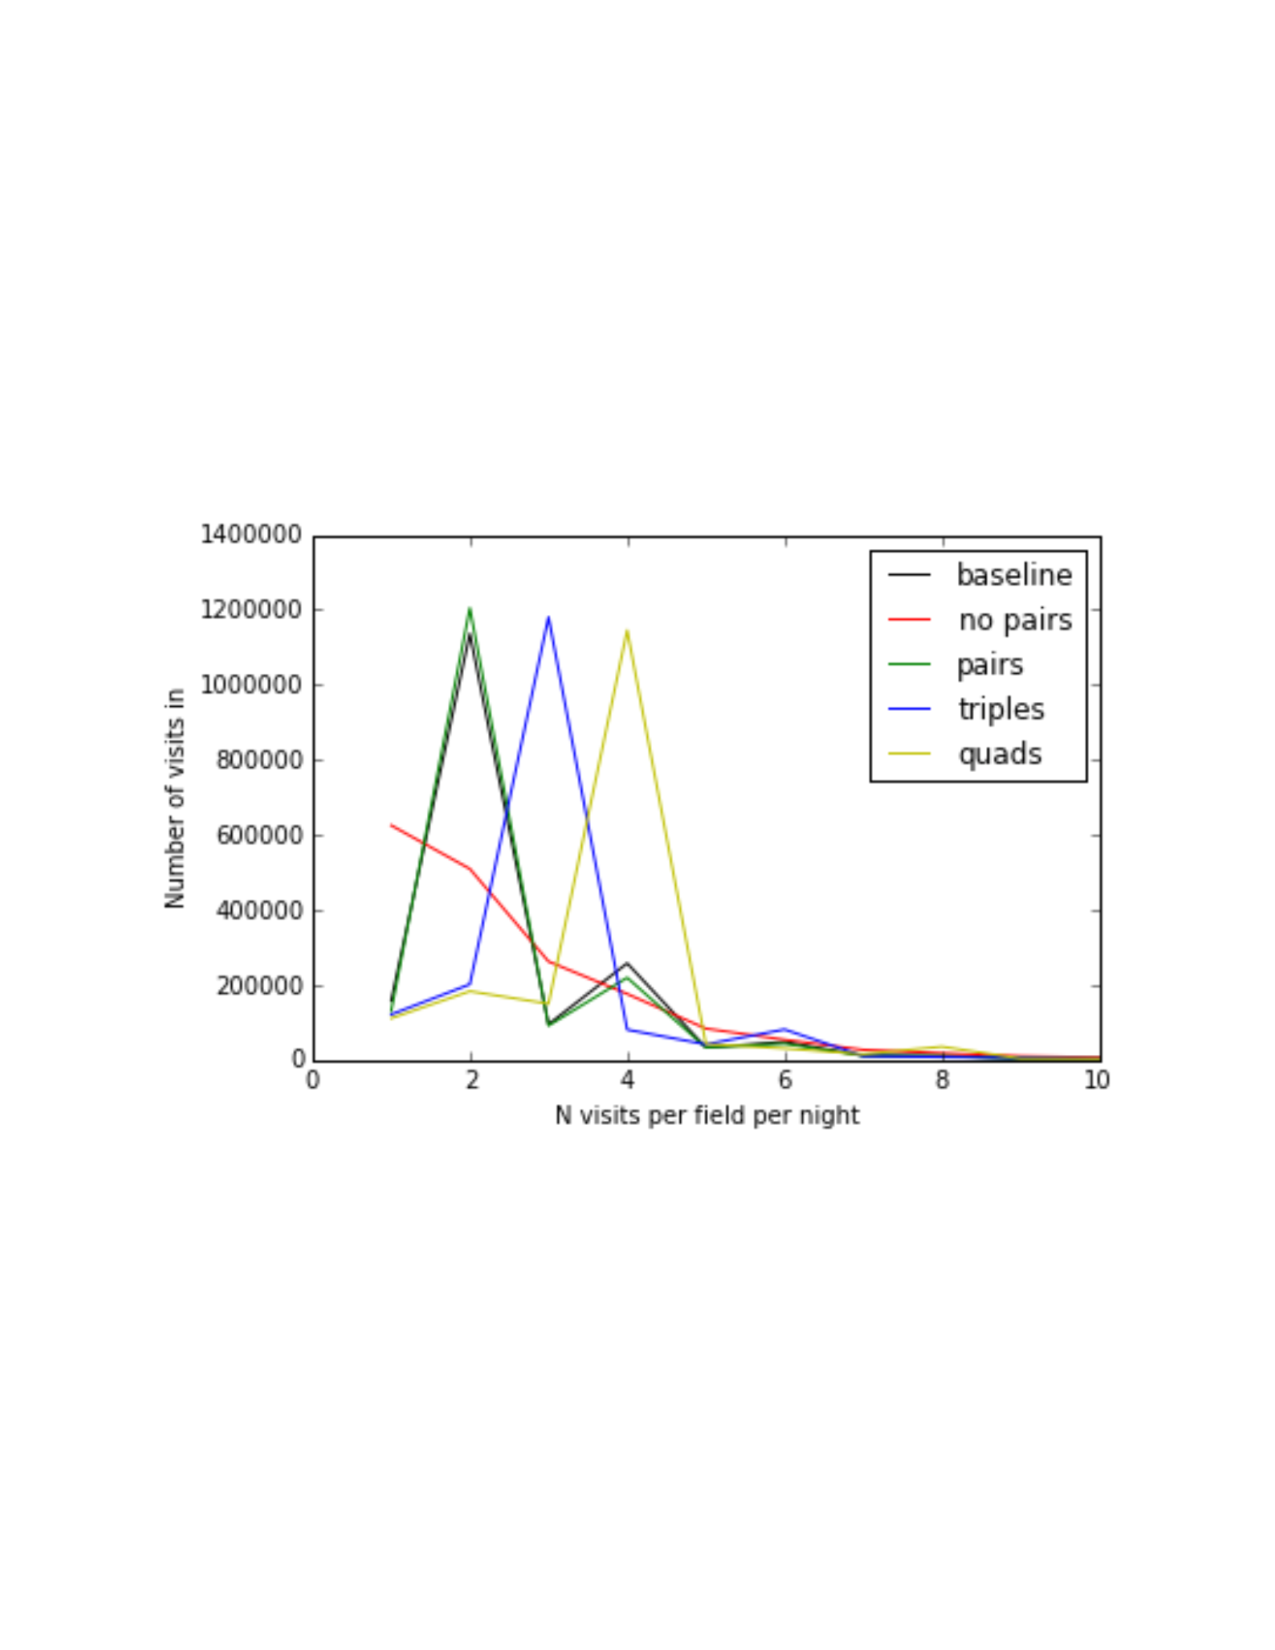
\includegraphics[angle=0,width=0.99\hsize:,clip]{figs/NvisitStats.pdf}
\vskip -2.7in
\caption{The distribution of the number of visits used for nightly sequences of
length given on the horizontal axis. Only $griz$ bands are used. Note that even
``no pairs'' simulation (\opsimdbref{db:NEOsNoVisitPairs})
includes multiple visits. The highest peak is at the
requested number of visits in a sequence.}
\label{fig:NvisitStats}
\end{figure}
%%%%%%%%%%%%%%%%%%%%%%%%%%%

%%%%%%%%%%%%%%%%%%%%%%%%%%%
\begin{figure}[t!]
\vskip -1.2in
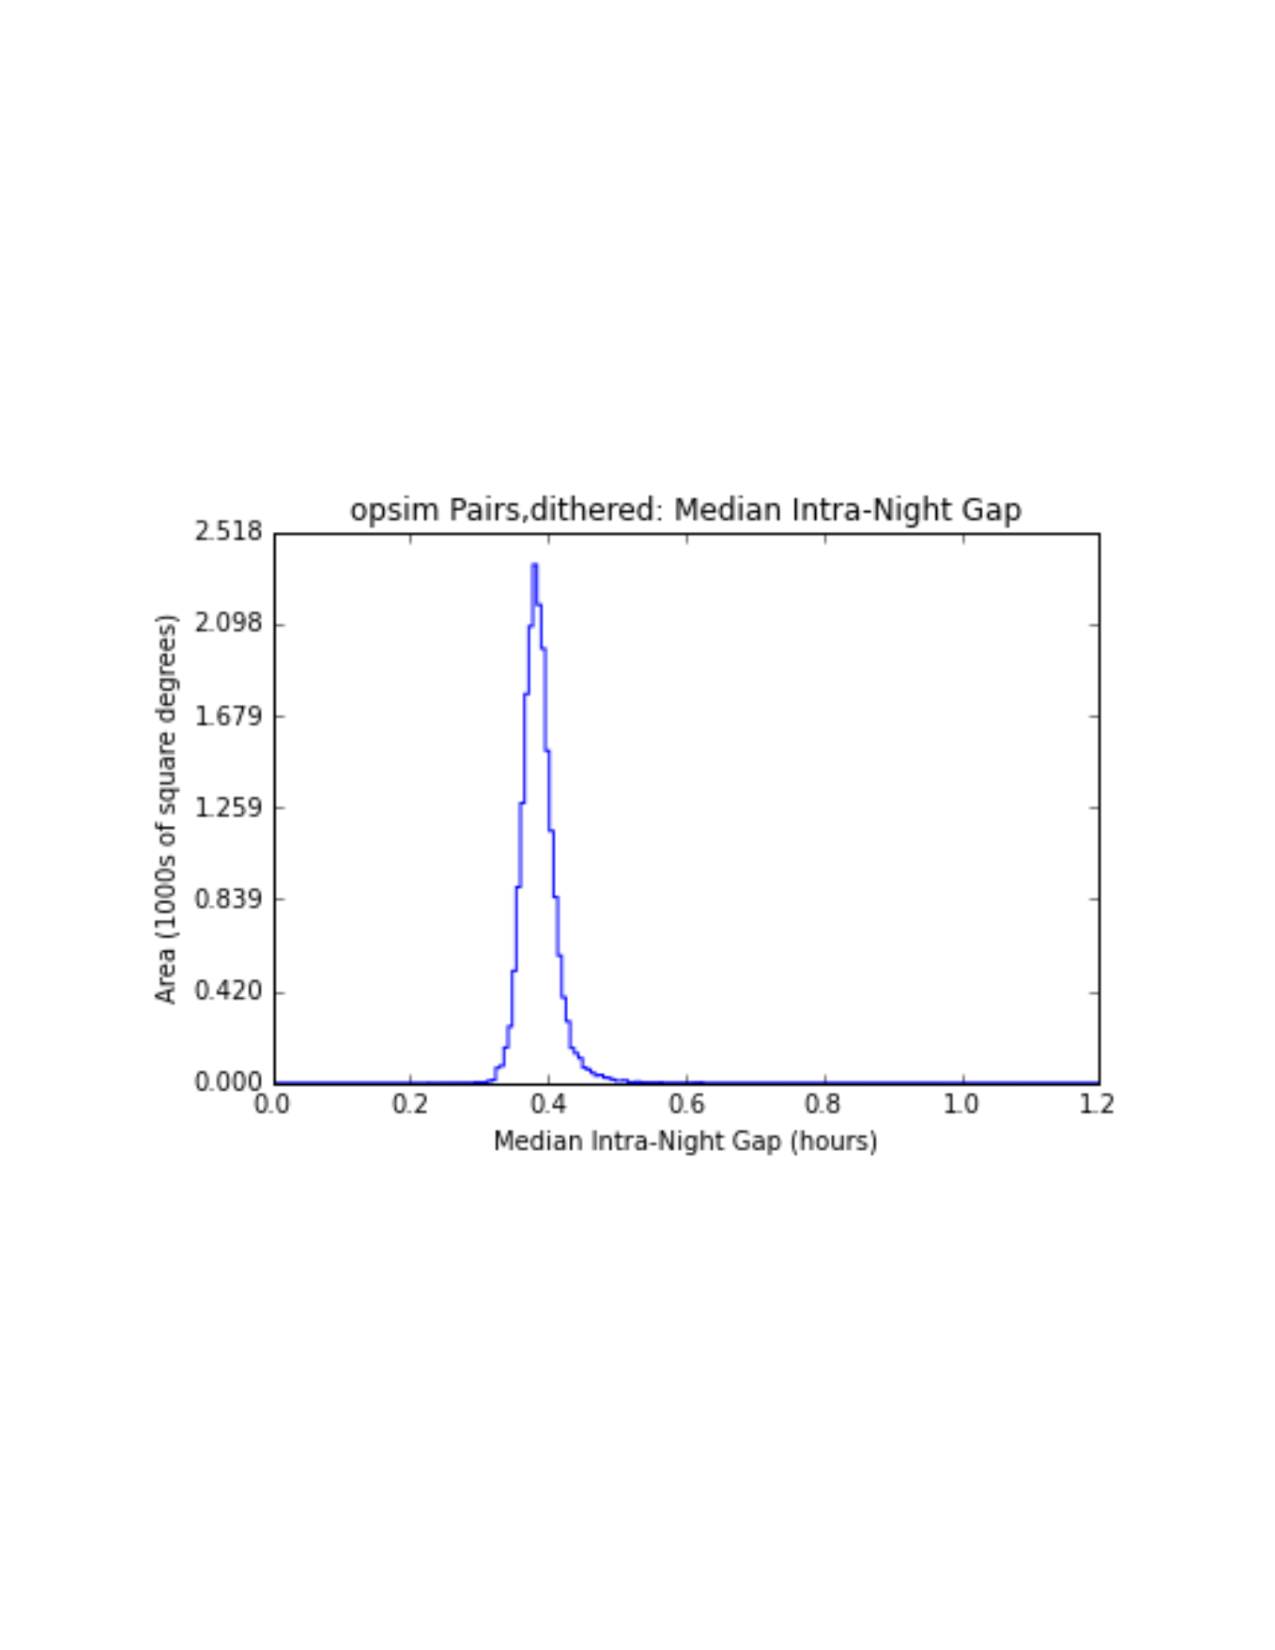
\includegraphics[angle=0,width=0.49\hsize:,clip]{figs/medinternight1.pdf}
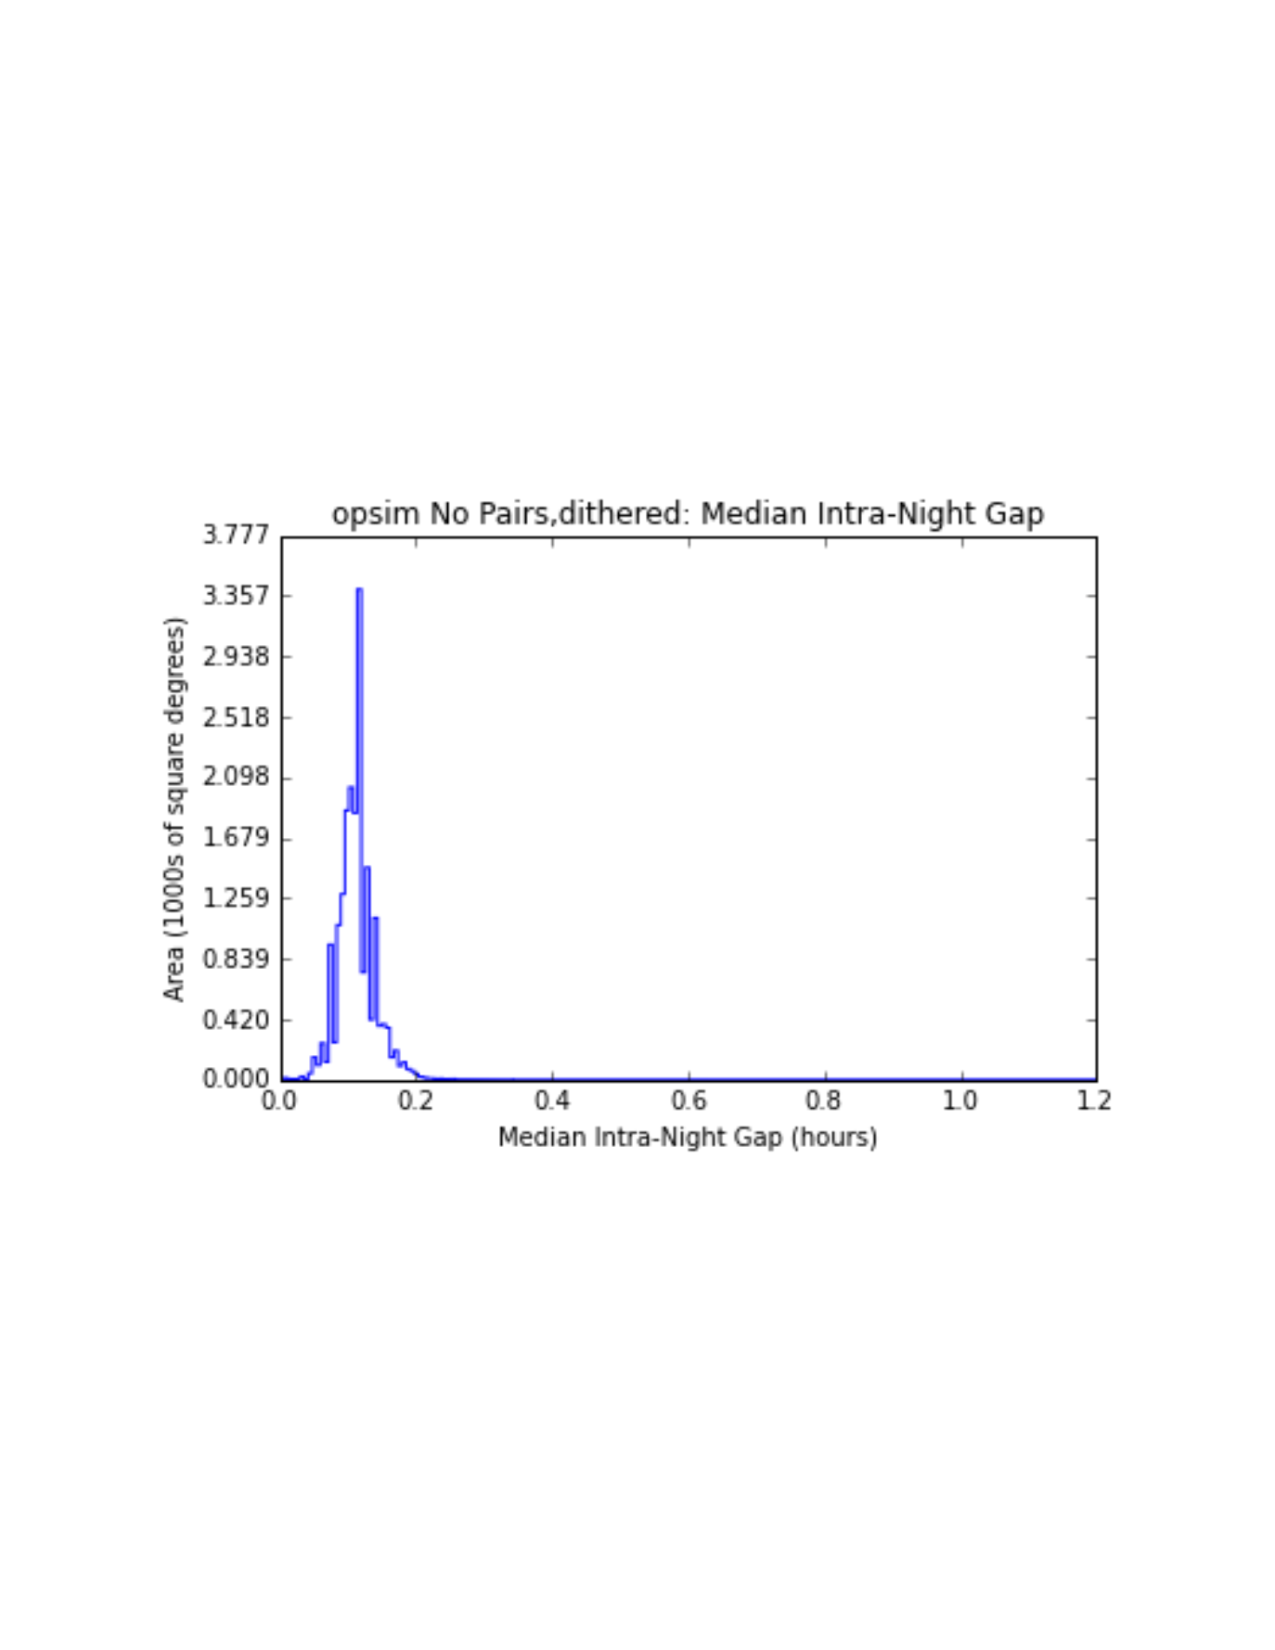
\includegraphics[angle=0,width=0.49\hsize:,clip]{figs/medinternight2.pdf}
\vskip -1.3in
\caption{
The comparison of the median intra-night gap distributions for Baseline Cadence (left)
and simulation \opsimdbref{db:NEOsNoVisitPairs}, which did not request pairs of visits per night.
Despite no need for pairs, simulation \opsimdbref{db:NEOsNoVisitPairs} produced them ``spontaneously'',
as well as longer sequences (see \autoref{fig:NvisitStats}). The mean field revisit
time is much shorter (about 6 minutes, see the right panel) than for Baseline Cadence
(22 minutes).}
\label{fig:intranightgapCompare}
\end{figure}
%%%%%%%%%%%%%%%%%%%%%%%%%%%

%%%%%%%%%%%%%%%%%%%%%%%%%%%
\begin{figure}[t!]
\vskip -1.1in
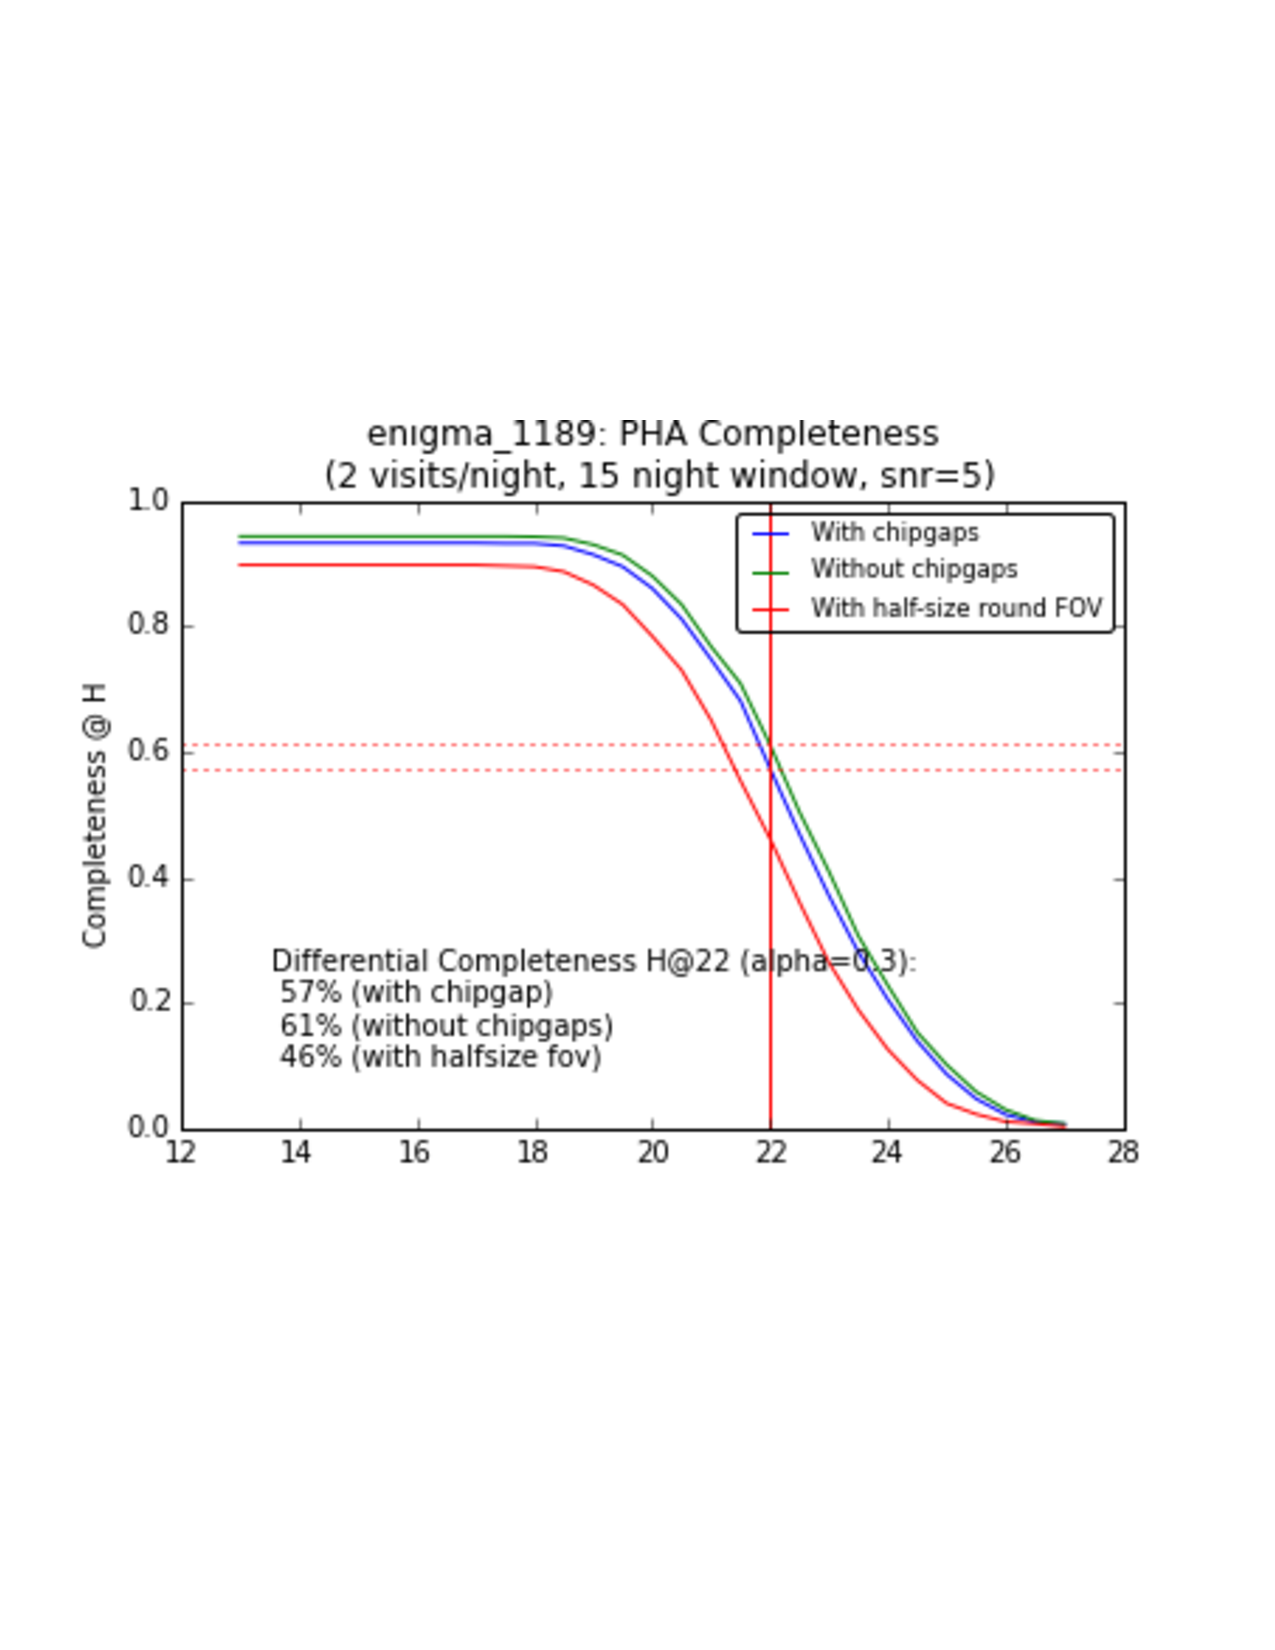
\includegraphics[angle=0,width=0.56\hsize:,clip]{figs/enigma1189_diffNEOcompleteness.pdf}
\hskip -0.5in
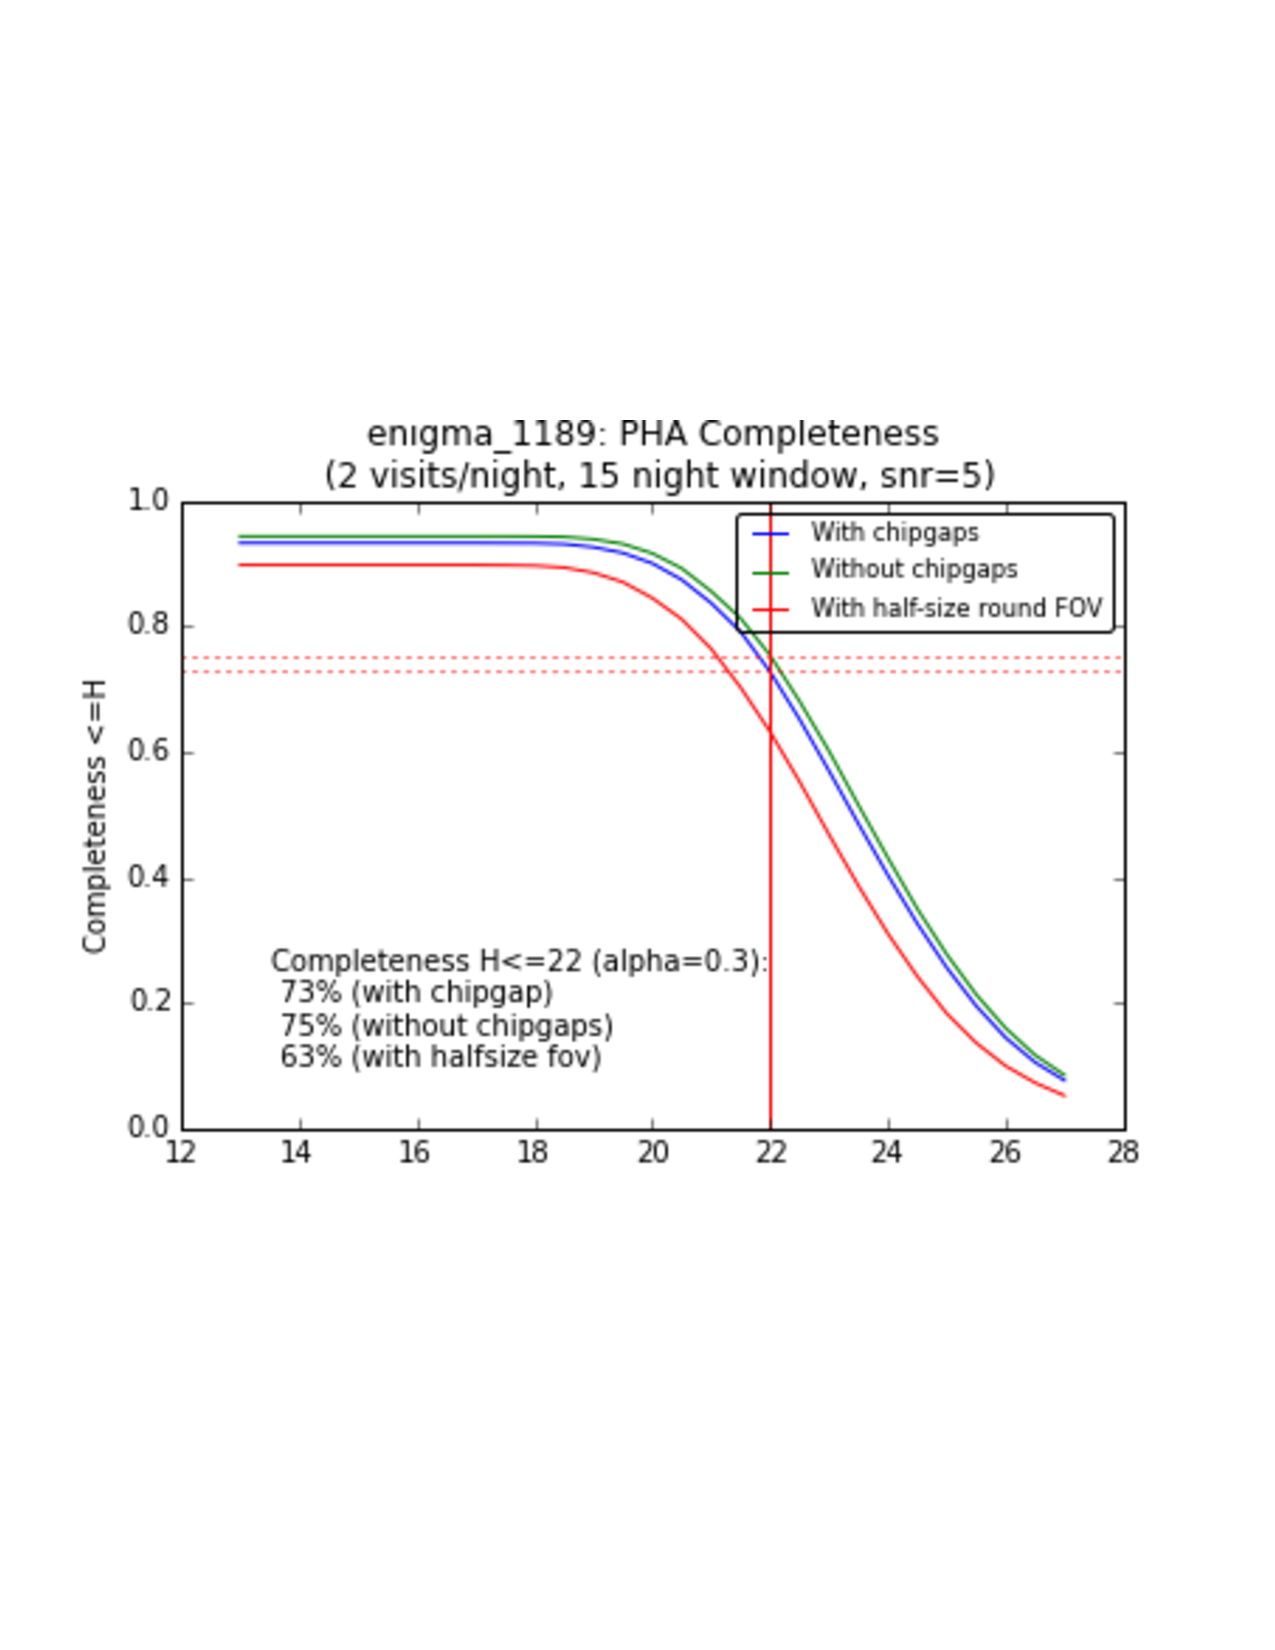
\includegraphics[angle=0,width=0.56\hsize:,clip]{figs/enigma1189_cumNEOcompleteness.pdf}
\vskip -1.2in
\caption{The PHA completeness for \opsimdbref{db:enigma}, as a function of the object's absolute
visual magnitude H on the horizontal axes (left: differential completeness at a given H;
right: cumulative completeness for all objects brighter than a given H).
The completeness for H$\le$22 NEOs (those with diameters larger than 140m)  for this
simulation is 73\% (blue line in the right panel). The panels also show the effects of ignoring
chip gaps (a 2\% effect for cumulative H$\le$22 completeness) and of decreasing the
field-of-view size to a half (i.e. to 4.8 sq. deg; a 10\% effect).}
\label{fig:enigmaNEO}
\end{figure}
%%%%%%%%%%%%%%%%%%%%%%%%%%%

%%%%%%%%%%%%%%%%%%%%%%%%%%%
\begin{figure}[th!]
\vskip -1.2in
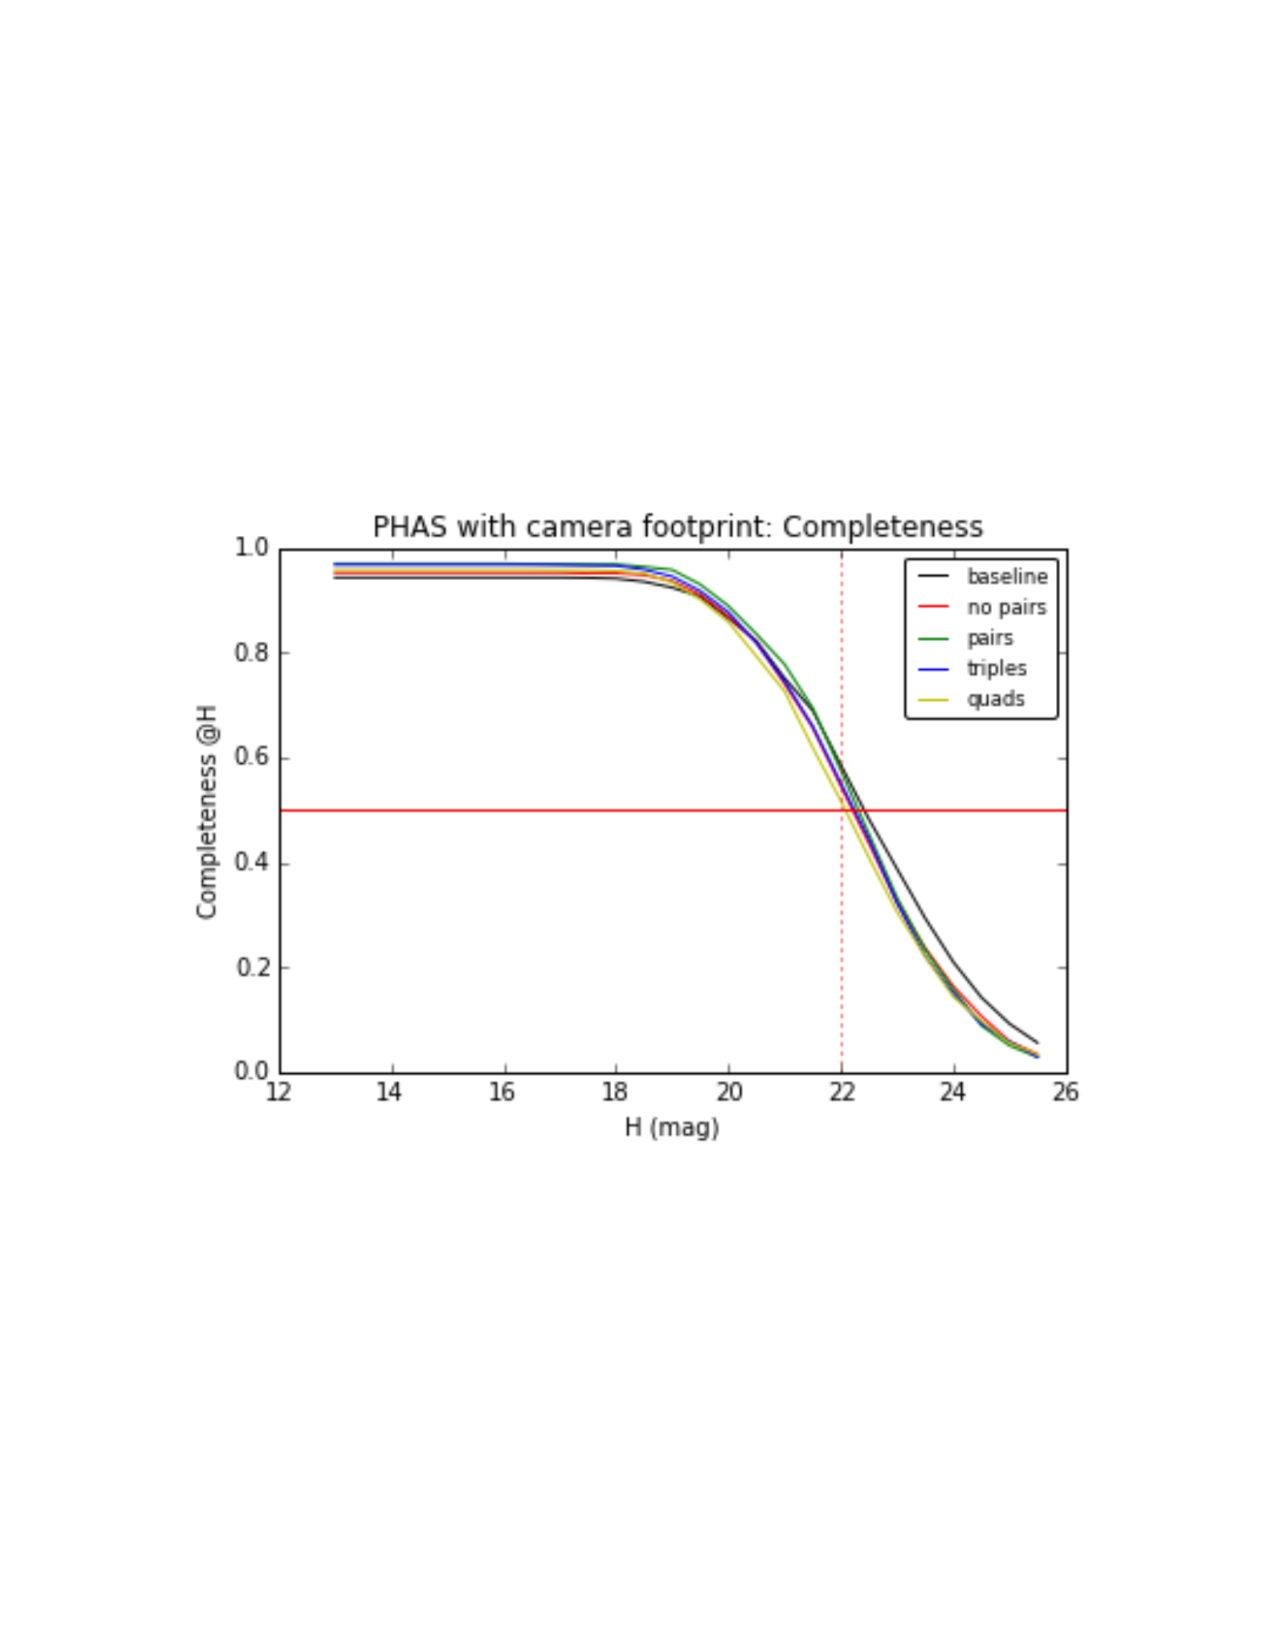
\includegraphics[angle=0,width=0.49\hsize:,clip]{figs/diffNEOpairs.pdf}
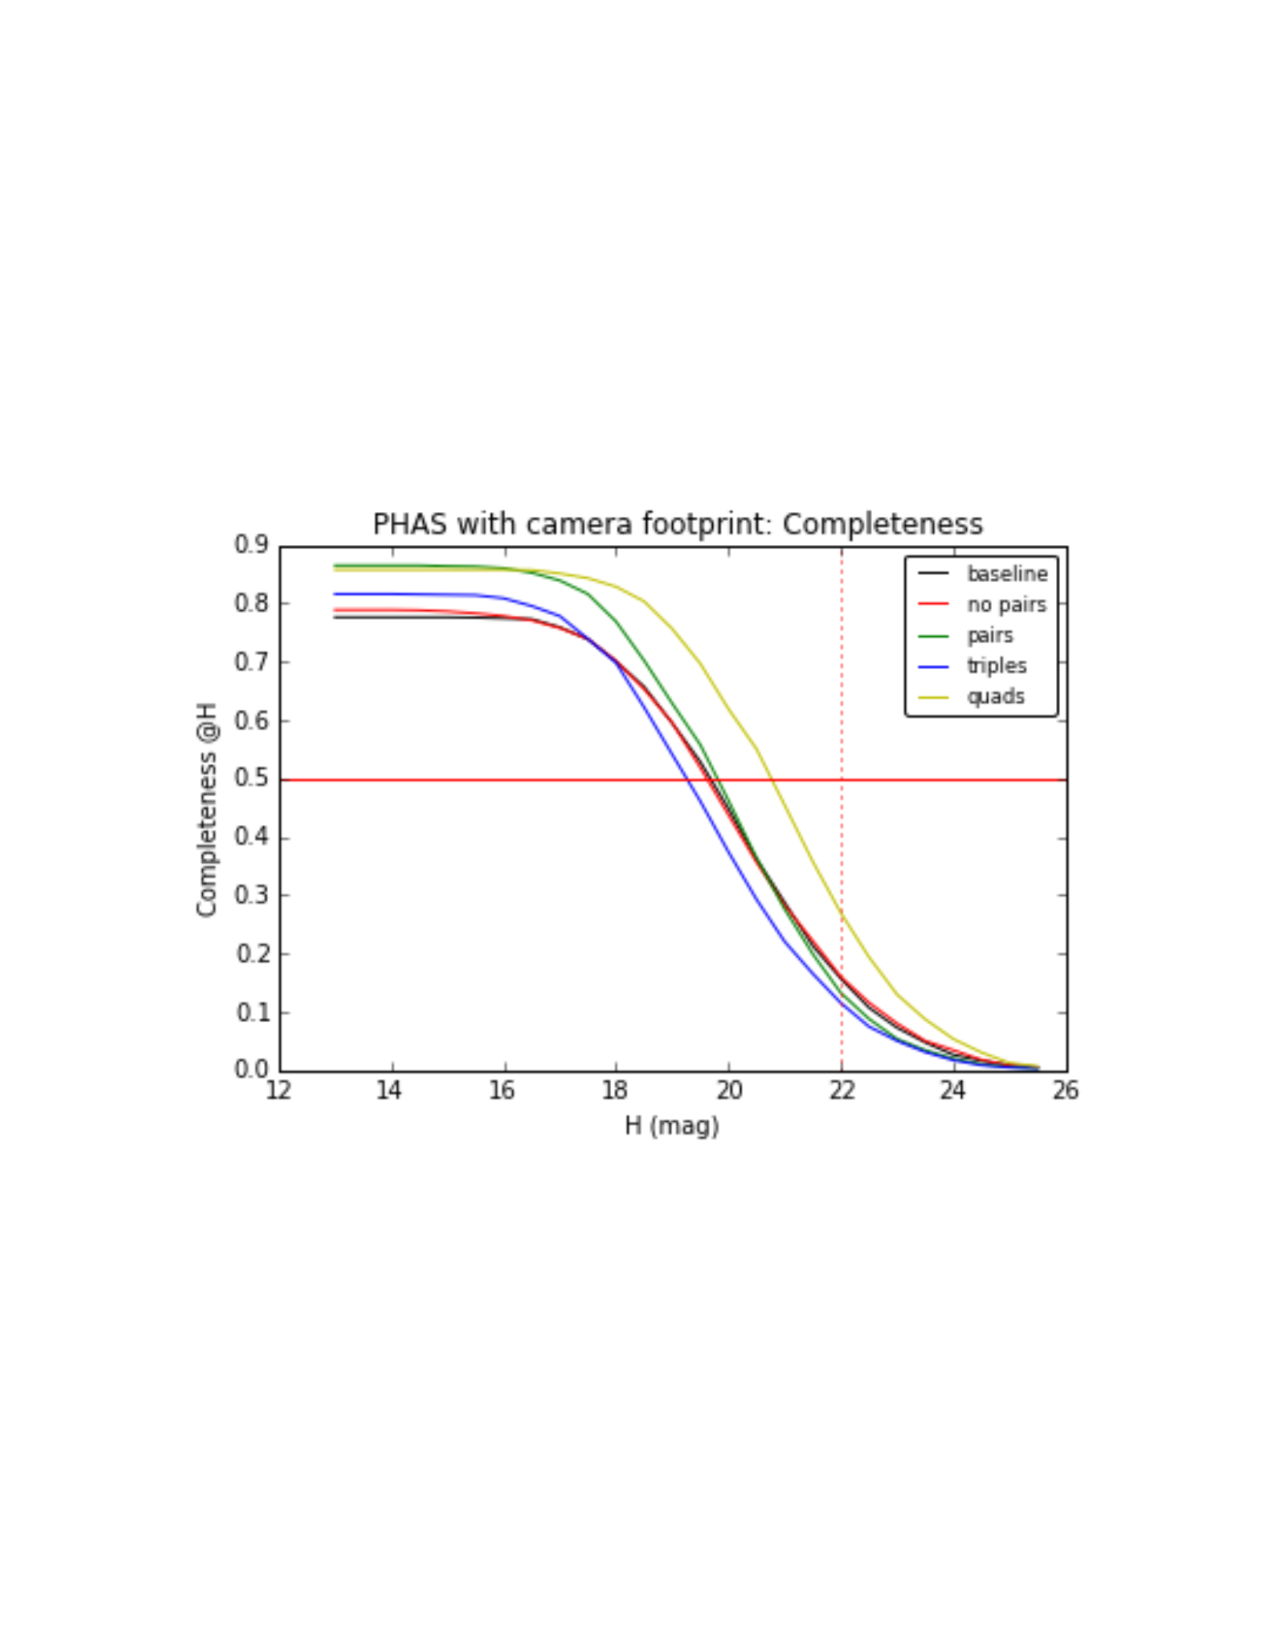
\includegraphics[angle=0,width=0.49\hsize:,clip]{figs/diffNEOquads.pdf}
\vskip -1.3in
\caption{
The comparison of differential PHA completeness for the five analyzed simulations
when requiring two detections per night (left) and four detections per night (right).
With two detections per night, all simulations perform similarly but when four
detections per night are required, the simulation that has the largest number
of such sequences (see \autoref{fig:NvisitStats}), performs the best although at an
inferior level compared to the left panel (see also \autoref{fig:enigmaNEO}).}
\label{fig:NEOquads}
\end{figure}
%%%%%%%%%%%%%%%%%%%%%%%%%%%


{\bf Analysis Results:}
First, we emphasize that ``requested'' is not the same as
``delivered'': even the ``no pairs''
simulation \opsimdbref{db:NEOsNoVisitPairs} ends
up having multiple visits in a given night to the same fields, and
when multiple visits per night are requested, not all fields get to
have completed sequences. The statistics of how many fields are
combined into sequences of a given number of visits is shown in
\autoref{fig:NvisitStats}.  As evident, the highest peak is at the
requested number of visits in a sequence, but not all visits are
incorporated into requested sequences: some are in both shorter and
longer sequences. In particular, even ``no pairs'' simulation includes
multiple visits to some fields, essentially because the current
version of the algorithm is not told not to do so. As illustrated in
\autoref{fig:intranightgapCompare}, such revisits typically happen
within 10 minutes from the first visit. This (unintended) behavior
implies that the naive expectation above is probably incorrect, as we
discuss in more detail below.


For baseline reference, the PHA completeness for
\opsimdbref{db:enigma} is shown in \autoref{fig:enigmaNEO}. The
baseline cadence achieves a cumulative completeness of 73\% for
H$\le$22 PHAs. This cumulative completeness for H$\le$22 is 17\%
higher than differential completeness at H=22 of 56\% due to
increasing completeness towards smaller H (larger objects). Both
differential and cumulative completeness are relevant metrics: the
former provides more insight in the behavior of a particular
simulation, while the latter is a metric given to NASA by the U.S.
Congress. Analysis of results illustrated in \autoref{fig:NEOquads}
can be summarized as follows:
\begin{itemize}
\item When NEO discovery algorithm requires pairs of visits, all runs
have very similar PHA completeness, with quads run only about 2\%
lower than the baseline (a differential completeness of 56\% at H=22
for \opsimdbref{db:enigma})
\item When NEO discovery algorithm requires 4 detections per night,
the simulation with quads achieves a differential completeness of
about 27\% at H=22, or  about 30\% lower completeness than Baseline
Cadence.
\item When NEO discovery algorithm requires 4 detections per night,
Baseline Cadence reaches a differential completeness of about 15\% at
H=22 (some quads are unintentionally produced by chance, see
\autoref{fig:NvisitStats}).
\item When NEO discovery algorithm requires 3 detections per night,
runs which requested triples and quads achieve a differential
completeness of about 40\% at H=22 (corresponding to a cumulative
completeness of about 57\% for H$\le$22).
\end{itemize}

Therefore, going from pairs of visits to triples (both for cadence and
NEO detection) reduces completeness (both differential and cumulative)
for PHAs with H$\le$22 by about 15-20\% (and by about 30\% for quads).


\subsubsection{Impact on other science programs}

The impact of requesting sequences with 3 or 4 visits to the same
field on other science programs is not yet analyzed in detail.  The
impact on static science should be minimal, except perhaps for a bit
worse behavior of various systematic errors (because fewer nights,
with their observing conditions, are sampled).

For time-domain science, the mean revisit time will increase by about
50\% if we go from pairs to triples, and by about a factor of two for
quads. This change will have a negative impact on time-domain science
programs based on SNe, variable stars, and transient objects, which
remains to be quantified.

\navigationbar

% --------------------------------------------------------------------

\section{Ongoing and Future Work}
\def\secname{cadexp:ongoing}\label{sec:\secname}


\subsection{Ongoing: Extended time-domain metrics}

A number of very sophisticated time-domain metrics have been
implemented in recent MAF development cycle (and some were contributed
by the community) but they have not been systematically run yet on all
available simulations. Time-domain metrics, together with metrics for
analyzing special programs (e.g. deep drilling programs), will be
further expanded in the next development cycle.


\subsection{Ongoing: Rolling Cadence experiments}

Analysis of a few prototype runs (\texttt{ops2\_1102},
\texttt{enigma\_1260}, \texttt{enigma\_1261}), which implemented the
so-called ``swiss cheese rolling cadence'' is in progress.


\subsection{Future work}

Based on analysis presented here, several recommendations
for further cadence exploration, can be made.

\begin{enumerate}

\item Further optimization of the main survey (e.g., exposure time in
general, and u band exposure time in particular; fixing western bias;
optimizing airmass limit and sky coverage; investigations of variable,
perhaps SNR-driven, exposure time).

\item Exploration and optimization of temporal sampling function in
general, and of Rolling Cadence in particular.

\item NEO completeness studies: what would it take for LSST to reach
90\% completeness for 140m and larger NEOs?  Based on previous
analysis, directions to explore are deeper visits along the Ecliptic
and longer survey duration (about 12 years).

\item Exploration of extending the main survey to the Galactic plane
(per A. Gould's proposal, arXiv:1304.3455) and further optimization of
Galactic plane and Bulge science programs.

\item Optimization of LMC/SMC coverage (and somewhat less importantly,
the South Celestial Pole coverage).

\item Deep drilling optimization (detailed analysis of existing
proposals; investigation of gains from going to a larger observing
time allocation, e.g. 20\%).

\item Twilight short-exposure time observing (per internal Stubbs proposal).

\item Planning commissioning observations (e.g. the tension between
going wide to enable self-calibration and dense temporal sampling to
obtain various light curve templates and fine tune image differencing
and multi-epoch data processing and data analysis software tools).

\item Dynamic cadence explorations (the main goal at this time is to
answer: are our tools good enough to act and react swiftly and
robustly in operations?).

\end{enumerate}

\navigationbar

% --------------------------------------------------------------------

\section{Summary}
\def\secname{cadexp:summary}\label{sec:\secname}

The most important conclusion of this study is that the upper limit on
possible scheduling efficiency improvements for Baseline Cadence is
close to 6\%. This conclusion is by and large based on the fact that
the mean slew time for (candidate) Baseline Cadence is 6.9 sec, and
thus only slightly larger than the design specifications for the
system slew and settle time of 4.5 sec.  Nevetheless, there are a
number of features to understand, and some to fix, and there is
substantial optimization potential in temporal sampling functions and
further optimization of the sky area and observing strategy details,
that can result in enhanced science even with the same integrated
open-shutter time (e.g. by obtaining deeper data through an improved
sampling of observing conditions).

\vskip 0.2in
The main other questions addressed here are:

\begin{enumerate}

\item {\it By what factor could we exceed the SRD design specification
for the number of visits if only Universal Cadence proposal was
implemented?}

A simulation that only implemented Universal Cadence proposal exceeded
the design specification for the number of visits by about 40\% (over
the design specification for the sky area of 18,000 sq.deg.)

\item {\it By what factor could we exceed the SRD design specification
for the sky coverage if only Universal Cadence proposal was
implemented with the design specification for the number of visits?}

This Pan-STARRS-like strategy results in about 40\% larger sky
coverage (about 25,000 sq.deg.), with the mean number of visits at
92\% of the design specification. The total number of visits is the
same as for Baseline Cadence, implying similar surveying efficiency.

Therefore, the available ``margin'' relative to the SRD design specifications
for the main survey is equivalent to about 30-40\% larger sky coverage, or
about 30-40\% more visits per field. The SRD assumes that 10\% margin
will be available for other programs. The implied ``survey reserve'',
relative to the Universal Cadence design specifications from the SRD, can
be used to:
  \begin{enumerate}
  \item increase the number of visits per field over the WFD area,  or
  \item increase the surveyed area while keeping the number of visits
  per field statistically unchanged, or
  \item increase both area and the number of visits, and/or
  \item execute additional programs (the current baseline).
  \end{enumerate}

\item {\it What is the effect of auxiliary proposals on surveying
efficiency?}

A comparison of simulations which only implemented Universal Cadence
proposal to those that included all other programs did not show a
significant change of efficiency (older simulations, not analyzed
here, showed increases in surveying efficiency of up to about 3\% due
to shorter slewing time).


\item {\it What is the effect of visit pairs on surveying efficiency? }

Relinquishing the visit pair requirement results in up to 2-3\%
improvement of the surveying efficiency. The impact on some
time-domain science would be positive, while for NEO and main-belt
asteroid science it would be strongly negative.


\item {\it Can the effects of variations of the visit exposure time on
surveying efficiency be predicted using simple efficiency estimates?}

Simple estimates based on comparing exposure (open shutter) and total
visit times are in good agreement with simulations. Decreasing the
visit exposure time to 20 seconds decreases the total open shutter
time by 10\%, and increasing it to 60 seconds increases the total open
shutter time by 16\%, relative to Baseline Cadence and standard
exposure time of 30 seconds. The number of visits changes by factors
of 1.35 and 0.58.


\item {\it What are the effects of doubling the exposure time only in
the $u$ band?}

The effect of doubling the exposure time only in the $u$ band, while
simultaneously halving the number of requested visits, has no
significant effect on the survey efficiency.

The effect of doubling the exposure time only in the $u$ band, with
the number of requested visits unchanged, is a decrease in the number
of visits in other bands by about 6\%.


\item {\it What is the impact of hard airmass limit, $X<1.5$, on the
surveying efficiency?}

It is a very bad idea to relax airmass limit! It is possible to
achieve the same surveying efficiency with much more stringent airmass
limit than 1.5, which was used in most simulations to date.

\end{enumerate}


\navigationbar


% --------------------------------------------------------------------

\chapter[Solar System]{Discovering and Characterizing Small Bodies in
  the Solar System}
\def\chpname{solarsystem}\label{chp:\chpname}

Chapter editors:
\credit{rhiannonlynne},
\credit{davidtrilling}.

% ====================================================================

\section{Introduction}
\label{sec:\chpname:intro}

LSST has tremendous potential as a discovery and characterization tool
for small bodies in the Solar System. With LSST, we have the
opportunity to increase our sample sizes of Potentially Hazardous
Asteroids (PHAs), Near Earth Objects (NEOs), Main Belt Asteroids
(MBAs), Jupiter Trojans, Centaurs, TransNeptunian Objects (TNOs),
Scattered Disk Objects (SDOs), comets and other small body populations
such as Earth mini-moons, irregular satellites, and other planetary
Trojan populations, by at least an order of
magnitude, often two orders of magnitude or more. In addition to
hundreds of astrometric measurements for most objects, LSST will also
provide precisely calibrated multiband photometry. With this
information, we can also characterize these populations -- deriving
colors, light curves, rotation periods, spin states, and even shape
models where possible.

The motivation behind studying these small body populations is
fundamentally to understand planet formation and evolution. The
orbital parameters of these populations record traces of the orbital
evolution of the giant planets. The migration of Jupiter, Saturn and
Neptune in particular have left marks on the orbital distribution of
MBAs, Jupiter Trojans, TNOs and SDOs. Rapid migration of
Jupiter and Saturn may have emplaced a large number of planetesimals
in the Scattered Disk; later slow migration of Neptune will affect the
number of TNOs in resonance and the details of their orbital parameters
within the resonance. Adding color information provides further
insights; colors roughly track composition, indicating formation
location and temperature or space weathering history. For example, the color
gradient of main belt asteroids, combined with their orbital
distribution, suggests that perhaps Jupiter migrated inwards,
mixing planetesimals from the outer Solar System into the outer parts
of the main belt, before eventually migrating outwards. Studying the
size distribution of each of the small body populations themselves
provides more constraints on planetesimal formation; this is
complicated by the effects of dynamical stirring from the giant
planets, which can increase the rate of erosion vs. growth during
collisions, and by the existence of the remnants of collisions such as
collisional families in the main belt. The presence of binaries and range
of spin states and shapes provides further constraints on the history
of each population. The location
of the planets before migration, the amount of migration, and the size
distribution of the small bodies themselves (after detangling the
dynamical evolution) all tell a deeper story about how the planets in
the Solar System formed, and how our formation history fits into the
range of observed extrasolar planetary systems.

These Solar System populations are unique when compared to other
objects which will be investigated by LSST, due to the simple fact
that they move across the sky. Metrics to evaluate
LSST's performance for moving objects need to be based on `per object'
measurements, rather than at a series of points on the sky or per
field pointing. For all metrics discussed in this chapter, the orbit
of each object is integrated over the time of the simulated opsim
survey and the times when each object is visible are recorded; these
series of observations per object are then the basis for metric
evaluations.

% Introduce, with a very broad brush, this chapter's science projects,
% and why it makes sense for them to be considered together.

% ====================================================================

\section{Discovering and linking Solar System Objects}
\def\secname{\chpname:discovery}\label{sec:\secname}

Discovering, rather than simply detecting, small objects throughout
the Solar System requires unambiguously linking a series of detections
together into an orbit. The orbit provides the information necessary
to scientifically characterize the object itself and to understand the
population as a whole. Without orbits, the detections of Solar System
Objects (SSOs) by LSST will be of limited use; objects discovered with
other facilities could be followed up by LSST, but almost the entire
science benefit to planetary astronomy would be lost. Linking and
orbit determination for Solar System objects is similar to source
association for non-moving objects; it provides the means to identify
multiple detections as coming from a single object.

Therefore, the first concern regarding the Solar System is related
to the question ``Can we link detections of moving objects into
orbits?''.  This requirement poses varying levels of difficulty as we
move from Near Earth Objects (NEOs) through the Main Belt Asteroids
(MBAs) and to TransNeptunian Objects (TNOs) and Scattered Disk Objects
(SDOs), as well as for comets and for other unusual but very
interesting populations such as Earth minimoons. Due to their small
heliocentric and geocentric distances, NEOs appear move with
relatively high velocities and are distributed over a large fraction
of the sky, far from the ecliptic plane. MBAs are densely distributed,
primarily within about 30 degrees of the ecliptic. TNOs and SDOs move
slowly, however short time intervals between repeat visits in each night may make these difficult
to link. Comets and Earth mini-moons may require more complicated
orbit fitting to allow for non-gravitational or geocentric orbits.

Much of the answer to this question comes down to the performance of
various pieces of LSST Data Management software. In particular,
important questions are the
rate of false positive detections resulting from difference imaging, the compute
limitations of the Moving Object Processing System (MOPS) to extend to high
apparent velocities, and the capability to unambiguously determine if
a linkage is `real' or not via orbit determination (done as part of
MOPS). Thus this question ranges beyond the limits of the OpSim simulated
surveys, but bears on the observing strategy requirements for
discovering Solar System Objects. An in-depth study of the performance
of difference imaging and MOPS is currently ongoing. However, we can
make a range of assumptions on how MOPS will perform and evaluate how
many and which objects can be linked under observational cadence, given those assumptions.


% --------------------------------------------------------------------

\subsection{Target measurements and discoveries}
\label{sec:\secname:targets}

Describe the discoveries and measurements you want to make. 

Now, describe their response to the observing strategy. Qualitatively,
how will the science project be affected by the observing schedule and 
conditions? In broad terms, how would we expect the observing strategy 
to be optimized for this science?





The baseline LSST criteria for `discovery' with MOPS are 2 detections per
night within 90 minutes (in order to create tracklets), repeated over
3 separate nights within 15 days (in order to link the tracklets into
tracks). With these 6 observations, it is assumed that orbit
determination will suffice to reject any false linkages. These are the
conditions that the ongoing study of MOPS will evaluate (given a
realistic set of LSST false-positive detections from difference
imaging). We can, however, also evaluate 

If we assume various detection requirements, ranging from XXX to the
minimum MOPS requirements, we can characterize the performance of
available simulated surveys in terms of their expected detection rates
for various known populations.

{\it describe completeness metrics for NEOs/MBAs/TNOs/etc - known
  populations. what do we do about unknown populations?}

Beyond this basic but absolutely critical requirement to actually
discover SSOs across the Solar System, we can start to look at other
science goals: detecting activity, determining colors for moving
objects, and measuring shapes and spin states for objects.

{\it describe requirements and challenges for these; why colors are
  hard, how many objects will we actually be able to determine
  shape/spin for, how lightcurves may differ from shape/spin}

Note: take a look at
\texttt{https://github.com/rhiannonlynne/MafSSO/blob/master/SSO\_Analysis.ipynb}
(an extremely messy ipython notebook, but starting to point at some of
the ideas I have for metrics -- let's expand on this)



% --------------------------------------------------------------------

\subsection{Metrics}
\label{sec:\secname:metrics}

Quantifying the response via MAF metrics: definition of the metrics,
and any derived overall figure of merit.


% --------------------------------------------------------------------

\subsection{OpSim Analysis}
\label{sec:\secname:analysis}

OpSim analysis: how good would the default observing strategy be, at
the time of writing for this science project?


% --------------------------------------------------------------------

\subsection{Discussion}
\label{sec:\secname:discussion}

Discussion: what risks have been identified? What suggestions could be
made to improve this science project's figure of merit, and mitigate
the identified risks?


% ====================================================================

\navigationbar

% ====================================================================

\section{Orbital Accuracy}
\def\secname{\chpname:discovery}\label{sec:\secname}

\credit{authorgithubname} % (Writing team)

% This individual section will need to describe the particular
% discoveries and measurements that are being targeted in this section's
% science case. It will be helpful to think of a ``science case" as a
% ``science project" that the authors {\it actually plan to do}. Then,
% the sections can follow the tried and tested format of an observing
% proposal: a brief description of the investigation, with references,
% followed by a technical feasibility piece. This latter part will need
% to be quantified using the MAF framework, via a set of metrics that
% need to be computed for any given observing strategy to quantify its
% impact on the described science case. Ideally, these metrics would be
% combined in a well-motivated figure of merit. The section can conclude
% with a discussion of any risks that have been identified, and how
% these could be mitigated.

A short preamble goes here. What's the context for this science
project? Where does it fit in the big picture?

% --------------------------------------------------------------------

\subsection{Target measurements and discoveries}
\label{sec:\secname:targets}

Describe the discoveries and measurements you want to make.

Now, describe their response to the observing strategy. Qualitatively,
how will the science project be affected by the observing schedule and
conditions? In broad terms, how would we expect the observing strategy
to be optimized for this science?


% --------------------------------------------------------------------

\subsection{Metrics}
\label{sec:\secname:metrics}

Quantifying the response via MAF metrics: definition of the metrics,
and any derived overall figure of merit.


% --------------------------------------------------------------------

\subsection{OpSim Analysis}
\label{sec:\secname:analysis}

OpSim analysis: how good would the default observing strategy be, at
the time of writing for this science project?


% --------------------------------------------------------------------

\subsection{Discussion}
\label{sec:\secname:discussion}

Discussion: what risks have been identified? What suggestions could be
made to improve this science project's figure of merit, and mitigate
the identified risks?


% ====================================================================

\section{Detecting Activity}
\def\secname{\chpname:discovery}\label{sec:\secname}

\credit{authorgithubname} % (Writing team)

% This individual section will need to describe the particular
% discoveries and measurements that are being targeted in this section's
% science case. It will be helpful to think of a ``science case" as a
% ``science project" that the authors {\it actually plan to do}. Then,
% the sections can follow the tried and tested format of an observing
% proposal: a brief description of the investigation, with references,
% followed by a technical feasibility piece. This latter part will need
% to be quantified using the MAF framework, via a set of metrics that
% need to be computed for any given observing strategy to quantify its
% impact on the described science case. Ideally, these metrics would be
% combined in a well-motivated figure of merit. The section can conclude
% with a discussion of any risks that have been identified, and how
% these could be mitigated.

A short preamble goes here. What's the context for this science
project? Where does it fit in the big picture?

How secure is the orbit - is it going to hit us?
Libration amplitude distribution for TNOs?
Can we find it after X years for further study?
Can we identify the source region for NEOs within the main belt?

% --------------------------------------------------------------------

\subsection{Target measurements and discoveries}
\label{sec:\secname:targets}

Describe the discoveries and measurements you want to make.

Now, describe their response to the observing strategy. Qualitatively,
how will the science project be affected by the observing schedule and
conditions? In broad terms, how would we expect the observing strategy
to be optimized for this science?


% --------------------------------------------------------------------

\subsection{Metrics}
\label{sec:\secname:metrics}

Quantifying the response via MAF metrics: definition of the metrics,
and any derived overall figure of merit.


% --------------------------------------------------------------------

\subsection{OpSim Analysis}
\label{sec:\secname:analysis}

OpSim analysis: how good would the default observing strategy be, at
the time of writing for this science project?


% --------------------------------------------------------------------

\subsection{Discussion}
\label{sec:\secname:discussion}

Discussion: what risks have been identified? What suggestions could be
made to improve this science project's figure of merit, and mitigate
the identified risks?

Different discussion / risks for each science case within this general metric?

% ====================================================================

\section{Detecting activity}
\def\secname{\chpname:discovery}\label{sec:\secname}

\credit{authorgithubname} % (Writing team)

% This individual section will need to describe the particular
% discoveries and measurements that are being targeted in this section's
% science case. It will be helpful to think of a ``science case" as a
% ``science project" that the authors {\it actually plan to do}. Then,
% the sections can follow the tried and tested format of an observing
% proposal: a brief description of the investigation, with references,
% followed by a technical feasibility piece. This latter part will need
% to be quantified using the MAF framework, via a set of metrics that
% need to be computed for any given observing strategy to quantify its
% impact on the described science case. Ideally, these metrics would be
% combined in a well-motivated figure of merit. The section can conclude
% with a discussion of any risks that have been identified, and how
% these could be mitigated.

A short preamble goes here. What's the context for this science
project? Where does it fit in the big picture?

% --------------------------------------------------------------------

\subsection{Target measurements and discoveries}
\label{sec:\secname:targets}

Describe the discoveries and measurements you want to make.

Now, describe their response to the observing strategy. Qualitatively,
how will the science project be affected by the observing schedule and
conditions? In broad terms, how would we expect the observing strategy
to be optimized for this science?


% --------------------------------------------------------------------

\subsection{Metrics}
\label{sec:\secname:metrics}

Quantifying the response via MAF metrics: definition of the metrics,
and any derived overall figure of merit.


% --------------------------------------------------------------------

\subsection{OpSim Analysis}
\label{sec:\secname:analysis}

OpSim analysis: how good would the default observing strategy be, at
the time of writing for this science project?


% --------------------------------------------------------------------

\subsection{Discussion}
\label{sec:\secname:discussion}

Discussion: what risks have been identified? What suggestions could be
made to improve this science project's figure of merit, and mitigate
the identified risks?

\navigationbar

% ====================================================================


% --------------------------------------------------------------------

\chapter[The Galaxy]{The Galaxy}
\def\chpname{galaxy}\label{chp:\chpname}

\noindent {\it
Will Clarkson, Kathy Vivas, Peregrine McGehee, and others to follow
}

% --------------------------------------------------------------------

\section{Introduction}
\def\secname{intro}\label{sec:\secname}

% WIC 2015-08-21 15:00: lots of edits to the intro text to refocus the
% document a bit more usefully.

LSST will significantly advance Milky Way science, on lengthscales
from the galactic halo and local volume, right down to sensitive
surveys for faint nearby objects to uncover the true state of the
Solar Neighborhood.
%The broad reach of the Milky Way science
%cases is nicely summarized in Section 2.1.4 of Ivezic et al. (2008
%arXiv 0805.2366).
%\begin{itemize}
%\item What is the detailed structure and accretion history of the Milky Way?
%\item What are the fundamental properties of all the stars within 300 pc of the Sun?
%\end{itemize}
Much more detail about most of these science cases, and specific
science questions to be answered, can be found in the LSST Science
Book (particularly chapters 6 and 7) and Ivezic et al. (2008 arXiv
0805.2366, in particular Sections 2.1.4 and 4.4); in this chapter we
(aim to) present metrics that will allow various observing strategies
to be quantitatively assessed in terms of their impact on science
cases falling under the general rubric of ``The Milky Way.''  

Our intention is to decouple the technical issue of coverage on-sky
from the science accomplished; for example, if a science case includes
regions both inside and outside of the ``Wide-Fast-Deep'' (WFD)
survey, then the metric for a particular science case should produce a
quantitative assessment of the science outcome no matter what the
distribution of pointings on the sky actually was. As a result, issues
to do with areal coverage (for example, whether a census of all nearby
brown dwarfs that neglects ``low-latitude'' fields towards the inner
Galaxy, is scientifically unacceptable) should in theory fall out as a
result of the metrics assessment process.

This chapter is organized as follows. In Section \ref{sec:GeneralMW}
we point out some general considerations specific to much of the Milky
Way science area that we recommend MW scientists bear in mind when
considering metrics. Because of the large diversity of science cases,
Section \ref{sec:SummaryTableMW} presents the essential aspects of
each science case, expressed in terms of observational goals and
tracer population. Science cases dominated by in-plane observations
are presented first in Table X, as the observing strategy for in-plane
observations is currently far from resolved. Then Table Y in this
section presents the vital statistics for science cases covered by
Wide-Fast-Deep. Sections
\ref{sec:MW_spatial_structure}-\ref{sec:MW_localvolume} then present
the metrics and their evaluations for MW science cases. Finally,
section \ref{sec:MW_future_work} points the way to anticipated future
improvements to this living document in light of expected precursor data.

\section{Some general considerations for Milky Way metrics}
\def\secname{GeneralMW}\label{sec:\secname}

Many of the Milky Way science cases involve Galactic Plane
observations almost exclusively. At the time of writing (late August
2015), even the broad parameters of in-plane observations remain to be
decided (for example the number of exposures per-filter).

Before launching into the specifics of metrics per-science case, we
point out some general factors that are likely to obtain for Milky Way
science (all over the sky), which we encourage the reader to
incorporate into their thinking when considering possible
metrics. [Language will change as metrics are produced.]

We currently envisage these to be implemented as methods that a given
science metric would call as part of its chain of evaluation.

{\it 1. Observing the ``foreground:''} By the standards of LSST's
Wide-Fast-Deep survey, many if not most of the objects of interest to
Milky Way science are close enough that they will saturate under the
Wide-Fast-Deep cadence, or will be impacted by bright foreground
objects. With LSST's saturation limit at 15 second exposure in the
neighborhood of $r \sim 17$~({\bf need confirmation!}), metrics should
include in their chain of evaluation, some sensitivity to at least the
following implications of foreground observation:

\begin{itemize}

  \item The upper limit on brightness for which measurements can be made that are sufficiently accurate for a given science case;
  
  \item The loss in discovery efficiency due to charge bleeds from objects unrelated to the targets for a given science case.
  
\end{itemize}

The discovery efficiency metric may correlate with existing
first-order metrics already presented elsewhere; for example, the
range of position angles for a field will likely correlate with the
discovery efficiency in the presence of charge bleeds, as a wider
range of position-angles will reduce the number of exposures in which
a given faint target lies underneath the charge bleed from one very
bright foreground object. Or, a given dithering strategy might
increase discovery efficiency due to pathological, very close, very
bright objects being moved into chip-gaps during some of the dithers.

(One suggested observing configuration for the Plane to mitigate the
impact of both of these factors, is to split the exposures per pair
into unequal-length exposures; perhaps $(1 \times 1s + 1\times 10s)$,
to ensure that nearly every object has an unsaturated exposure in
nearly every field. Although we do not wish to suggest a large array
of observing strategies at this stage, we do recommend that this
option be simulated for in-plane observations.)

{\it 2: Crowding and seeing:} Metrics for in-plane science must
incorporate the impact of spatial confusion on both photometric and
astrometric measurements. Both of these depend on seeing. More work
remains to be done on the level of sophistication necessary in these
considerations; for example, when considering relative proper motion
precision, the spatial density of reference stars at similar
brightness to the object whose proper motion is desired (to mitigate
magnitude-dependent PSF effects like the ``fatter-brighter'' effect)
will in principle impact the proper motion precision attainable. The
size of the impact of this effect on proper motion precision should be
determined.

{\it 3: Relative and absolute metrics:} Because even the first-order
observation parameters for in-plane observations are somewhat
unconstrained, metrics should be sensitive to differences in overall
allocation as well as by comparison to the ideal strategy within an
allocation. For example, the way in which observations are distributed
within a time baseline is not very impactful to many science cases if
that baseline is only three years long for OpSim algorithmic reasons!
(For example, OpSim might move all the exposures in a galactic plane
science case into the first three years to finish short projects
early, which would be a disaster for cases that require a long time
baseline.)

\section{Summary table of Milky Way science cases}
\def\secname{SummaryTableMW}\label{sec:\secname}

Here we present a quick-look summary of the Milky Way science cases
to-date, with measurement type and tracer population indicated where
appropriate. This communicates the importance of certain objects and
certain regimes to Milky Way science. Given the considerations
outlined in Section \ref{sec:GeneralMW}, this overview is split in two
tables: Table 1 shows science cases for the five main science cases we
have identified for metric development, while while Table Y summarizes
the rest in terms of tracers and simple scaling relations (the
majority of which can safely assume SRD performance numbers).

{\bf All those bullet points from v1 of this chapter are condensed and summarized in these tables.}

[Table 1 - measurements and tracers for the five main science cases requiring new metrics.]

[Table 2 - Milky Way science cases not in Table 1; scaling relations from other metrics.]

({\it Hierarchical metrics (e.g. github Issue \#79):} since others are
developing detailed metrics for fine-grained issues of detectability,
in this Chapter we focus our candidate metrics mostly on high-level
metrics that might call the variability metrics as functions.) 

The following sections describe observing metrics for Milky Way
science cases. These have signficant (but not exclusive)
observation-sets in or towards the Plane. If your science case is not
mentioned below, it should be mentioned concisely in Table 2.


% Subsection filenames all start with ``MW'' in violation of Phil's
% advice to avoid chapter-specific names. This is to avoid namespace
% collision between ``microlensing'' for AGN and ``microlensing'' in
% the MW, for example!

Section \ref{sec:MW_spatial_structure}: The spatial structure of the Milky Way Galaxy, including the plane, bulge, halo and local volume;

Section \ref{sec:MW_metallicity_mapping}: Metallicity and age mapping in the Milky Way; 

Section \ref{sec:MW_SFH}: Star formation history of the Milky Way;

Section \ref{sec:MW_Dust}: Dust in the Milky Way;

Section \ref{sec:MW_microlensing} Microlensing;

Section \ref{sec:MW_Plane} Galactic Plane Science---Case for DWF;

% There may be one more section here: stellar populations of interest
% with unknown scale-heights. Chuck Claver's white dwarf pulsator
% project might be of interest here, among others.

%{\it Milky Way science cases but mostly in Wide-Fast-Deep:}

%Section \ref{sec:solarneighborhood} The Solar Neighborhood;

%Section \ref{sec:starclusters} Star Clusters in the Milky Way;

%Section \ref{sec:halostructure} Halo structure and populations;

%Section \ref{sec:localvolume} The Local Volume

[As of 2015-08-21, the .tex files for these subsections are mostly
  empty shells. Content to follow.]

[To be resolved: how to ensure Solar Neighborhood science is best represented. Does this deserve a sixth section?]

\input{MilkyWay/MW_spatial_structure.tex}
% ====================================================================
%+
% SECTION:
%    section-name.tex  % eg lenstimedelays.tex
%
% CHAPTER:
%    chapter.tex  % eg cosmology.tex
%
% ELEVATOR PITCH:
%    Explain in a few sentences what the relevant discovery or
%    measurement is going to be discussed, and what will be important
%    about it. This is for the browsing reader to get a quick feel
%    for what this section is about.
%
% COMMENTS:
%
%
% BUGS:
%
%
% AUTHORS:
%    Phil Marshall (@drphilmarshall)  - put your name and GitHub username here!
%-
% ====================================================================

\section{Metallicity and age mapping in the Milky Way}
\def\secname{MW_metallicity_mapping}\label{sec:\secname} % For example, replace "keyword" with "lenstimedelays"

\noindent{\it Author Name(s)} % (Writing team)

% This individual section will need to describe the particular
% discoveries and measurements that are being targeted in this section's
% science case. It will be helpful to think of a ``science case" as a
% ``science project" that the authors {\it actually plan to do}. Then,
% the sections can follow the tried and tested format of an observing
% proposal: a brief description of the investigation, with references,
% followed by a technical feasibility piece. This latter part will need
% to be quantified using the MAF framework, via a set of metrics that
% need to be computed for any given observing strategy to quantify its
% impact on the described science case. Ideally, these metrics would be
% combined in a well-motivated figure of merit. The section can conclude
% with a discussion of any risks that have been identified, and how
% these could be mitigated.

A short preamble goes here. What's the context for this science
project? Where does it fit in the big picture?

% --------------------------------------------------------------------

\subsection{Target measurements and discoveries}
\label{sec:keyword:targets}

Describe the discoveries and measurements you want to make.

Now, describe their response to the observing strategy. Qualitatively,
how will the science project be affected by the observing schedule and
conditions? In broad terms, how would we expect the observing strategy
to be optimized for this science?


% --------------------------------------------------------------------

\subsection{Metrics}
\label{sec:keyword:metrics}

Quantifying the response via MAF metrics: definition of the metrics,
and any derived overall figure of merit.


% --------------------------------------------------------------------

\subsection{OpSim Analysis}
\label{sec:keyword:analysis}

OpSim analysis: how good would the default observing strategy be, at
the time of writing for this science project?


% --------------------------------------------------------------------

\subsection{Discussion}
\label{sec:keyword:discussion}

Discussion: what risks have been identified? What suggestions could be
made to improve this science project's figure of merit, and mitigate
the identified risks?


% ====================================================================

\navigationbar

% ====================================================================
%+
% SECTION:
%    section-name.tex  % eg lenstimedelays.tex
%
% CHAPTER:
%    chapter.tex  % eg cosmology.tex
%
% ELEVATOR PITCH:
%    Explain in a few sentences what the relevant discovery or
%    measurement is going to be discussed, and what will be important
%    about it. This is for the browsing reader to get a quick feel
%    for what this section is about.
%
% COMMENTS:
%
%
% BUGS:
%
%
% AUTHORS:
%    Phil Marshall (@drphilmarshall)  - put your name and GitHub username here!
%-
% ====================================================================

\section{Star Formation History of the Milky Way}
\def\secname{MW_SFH}\label{sec:\secname} % For example, replace "keyword" with "lenstimedelays"

\noindent{\it Author Name(s)} % (Writing team)

% This individual section will need to describe the particular
% discoveries and measurements that are being targeted in this section's
% science case. It will be helpful to think of a ``science case" as a
% ``science project" that the authors {\it actually plan to do}. Then,
% the sections can follow the tried and tested format of an observing
% proposal: a brief description of the investigation, with references,
% followed by a technical feasibility piece. This latter part will need
% to be quantified using the MAF framework, via a set of metrics that
% need to be computed for any given observing strategy to quantify its
% impact on the described science case. Ideally, these metrics would be
% combined in a well-motivated figure of merit. The section can conclude
% with a discussion of any risks that have been identified, and how
% these could be mitigated.

Summary: this important topic does not seem to have been developed in
previous versions of the LSST science book or Ivezic et
al. (2008). LSST gives the opportunity to survey extensive areas
around star formation regions in the Southern hemisphere. Among
others, it would allow to study the Initial Mass Function down to the
sub-stellar limit across different environments. Young stars are
efficiently identified by their variability.

A short preamble goes here. What's the context for this science
project? Where does it fit in the big picture?

% --------------------------------------------------------------------

\subsection{Target measurements and discoveries}
\label{sec:keyword:targets}

In order to assess the ability of LSST to 1) identify and 2) classify
YSO we need to quantify the variability timescales and amplitudes of
both Class I/II (stars with disks) and Class III (WTTS). Inclusion of
eruptive variables (FUor/Exor) is appropriate as well - see section
8.10.2 in the Science Book.

In brief, WTTS are quasi-periodic with amplitudes of 0.1 to 0.3 mag
and periods 1 to ~15 days - so comparable to gamma Dor stars (see
Figure 8.17 in the SB). Given the temporal evolution of cool spots, a
period recovery analysis such as shown for RRL stars (se FIgure 8.20
in the SB) is likely difficult. The embedded systems and CTTS are
irregular variables but shown have distinctive colors due to
extinction + UB/blue excess arising from to accretion shocks.


%Describe the discoveries and measurements you want to make.

%Now, describe their response to the observing strategy. Qualitatively,
%how will the science project be affected by the observing schedule and
%conditions? In broad terms, how would we expect the observing strategy
%to be optimized for this science?


% --------------------------------------------------------------------

\subsection{Metrics}
\label{sec:keyword:metrics}

Quantifying the response via MAF metrics: definition of the metrics,
and any derived overall figure of merit.


% --------------------------------------------------------------------

\subsection{OpSim Analysis}
\label{sec:keyword:analysis}

OpSim analysis: how good would the default observing strategy be, at
the time of writing for this science project?


% --------------------------------------------------------------------

\subsection{Discussion}
\label{sec:keyword:discussion}

Discussion: what risks have been identified? What suggestions could be
made to improve this science project's figure of merit, and mitigate
the identified risks?


% ====================================================================

\navigationbar

% ====================================================================
%+
% SECTION:
%    section-name.tex  % eg lenstimedelays.tex
%
% CHAPTER:
%    chapter.tex  % eg cosmology.tex
%
% ELEVATOR PITCH:
%    Explain in a few sentences what the relevant discovery or
%    measurement is going to be discussed, and what will be important
%    about it. This is for the browsing reader to get a quick feel
%    for what this section is about.
%
% COMMENTS:
%
%
% BUGS:
%
%
% AUTHORS:
%    Phil Marshall (@drphilmarshall)  - put your name and GitHub username here!
%-
% ====================================================================

\section{Dust in the Milky Way}
\def\secname{MW_Dust}\label{sec:\secname} % For example, replace "keyword" with "lenstimedelays"

\noindent{\it Author Name(s)} % (Writing team)

% This individual section will need to describe the particular
% discoveries and measurements that are being targeted in this section's
% science case. It will be helpful to think of a ``science case" as a
% ``science project" that the authors {\it actually plan to do}. Then,
% the sections can follow the tried and tested format of an observing
% proposal: a brief description of the investigation, with references,
% followed by a technical feasibility piece. This latter part will need
% to be quantified using the MAF framework, via a set of metrics that
% need to be computed for any given observing strategy to quantify its
% impact on the described science case. Ideally, these metrics would be
% combined in a well-motivated figure of merit. The section can conclude
% with a discussion of any risks that have been identified, and how
% these could be mitigated.

{\it Peregrine's contribution appears to be missing here... was this overwritten in a commit since August?}\\

A short preamble goes here. What's the context for this science
project? Where does it fit in the big picture?

% --------------------------------------------------------------------

\subsection{Target measurements and discoveries}
\label{sec:keyword:targets}

Describe the discoveries and measurements you want to make.

Now, describe their response to the observing strategy. Qualitatively,
how will the science project be affected by the observing schedule and
conditions? In broad terms, how would we expect the observing strategy
to be optimized for this science?


% --------------------------------------------------------------------

\subsection{Metrics}
\label{sec:keyword:metrics}

Quantifying the response via MAF metrics: definition of the metrics,
and any derived overall figure of merit.

{\bf Metric 1: Uncertainty and bias in $E(B-V)$~estimates as a
  function of location on-sky.} Dependencies:

\begin{itemize}
  \item Stellar population throughout the survey (e.g. Knut / Peter developments; TRILEGAL?);
    \item Dust map throughout the survey region;
    \item Scale photometric error predictions for each band from program requirements per exposure;
      \item Produce formal estimate on the error in extinction and reddening as a function of position on-sky within the survey.
\end{itemize}


% --------------------------------------------------------------------

\subsection{OpSim Analysis}
\label{sec:keyword:analysis}

OpSim analysis: how good would the default observing strategy be, at
the time of writing for this science project?


% --------------------------------------------------------------------

\subsection{Discussion}
\label{sec:keyword:discussion}

Discussion: what risks have been identified? What suggestions could be
made to improve this science project's figure of merit, and mitigate
the identified risks?


% ====================================================================

\navigationbar

% ====================================================================
%+
% SECTION:
%    section-name.tex  % eg lenstimedelays.tex
%
% CHAPTER:
%    chapter.tex  % eg cosmology.tex
%
% ELEVATOR PITCH:
%    Explain in a few sentences what the relevant discovery or
%    measurement is going to be discussed, and what will be important
%    about it. This is for the browsing reader to get a quick feel
%    for what this section is about.
%
% COMMENTS:
%
%
% BUGS:
%
%
% AUTHORS:
%    Phil Marshall (@drphilmarshall)  - put your name and GitHub username here!
%-
% ====================================================================

\section{Microlensing in the Milky Way with LSST}
\def\secname{MW_microlensing}\label{sec:\secname} % For example, replace "keyword" with "lenstimedelays"

\noindent{\it Author Name(s)} % (Writing team)

% This individual section will need to describe the particular
% discoveries and measurements that are being targeted in this section's
% science case. It will be helpful to think of a ``science case" as a
% ``science project" that the authors {\it actually plan to do}. Then,
% the sections can follow the tried and tested format of an observing
% proposal: a brief description of the investigation, with references,
% followed by a technical feasibility piece. This latter part will need
% to be quantified using the MAF framework, via a set of metrics that
% need to be computed for any given observing strategy to quantify its
% impact on the described science case. Ideally, these metrics would be
% combined in a well-motivated figure of merit. The section can conclude
% with a discussion of any risks that have been identified, and how
% these could be mitigated.

%{\bf Note: these metrics have already been worked out in some detail
%  by Gould (arXiv). We do not expect to re-invent that wheel here.}

%A short preamble goes here. What's the context for this science
%project? Where does it fit in the big picture?

Gould (2013) argues assertively for inclusion of microlensing in the
Galactic plane as part of LSST core science; see also Section 4.8.

%Low-mass objects 


% --------------------------------------------------------------------

\subsection{Target measurements and discoveries}
\label{sec:keyword:targets}

Describe the discoveries and measurements you want to make.

Now, describe their response to the observing strategy. Qualitatively,
how will the science project be affected by the observing schedule and
conditions? In broad terms, how would we expect the observing strategy
to be optimized for this science?


% --------------------------------------------------------------------

\subsection{Metrics}
\label{sec:keyword:metrics}

Quantifying the response via MAF metrics: definition of the metrics,
and any derived overall figure of merit.

{\bf Metric 1: fraction of low-mass objects correctly triggered based
  on LSST observational timing.} Dependencies:
\begin{itemize}
  \item How many observations are required for an accurate trigger for followup? (E.g. could simply develop the ``Triples'' of Lund et al. (2015) towards higher number of repeat visits?) 
\item What is the minimum coverage of a microlensing event lightcurve before it is classified as detected and triggered for followup? 
\end{itemize}

{\bf Metric 2: Error on mass function of microlensing objects as a population.} Dependencies in addition to Metric 1, all as spatial map:
\begin{itemize}
  \item Capability to simulate microlens population under assumptions on the mass function
  \item Impact of sampling the mass function on its determination (e.g. if strategy X preferentially misses the short end of the timescale distribution, what does this do to the mass function determination?)
\end{iemize}



% --------------------------------------------------------------------

\subsection{OpSim Analysis}
\label{sec:keyword:analysis}

OpSim analysis: how good would the default observing strategy be, at
the time of writing for this science project?


% --------------------------------------------------------------------

\subsection{Discussion}
\label{sec:keyword:discussion}

Discussion: what risks have been identified? What suggestions could be
made to improve this science project's figure of merit, and mitigate
the identified risks?


% ====================================================================

\navigationbar

% ====================================================================
%+
% SECTION:
%    MW_Plane.tex
%
% CHAPTER:
%    .tex  % eg cosmology.tex
%
% ELEVATOR PITCH:
%    
% The Plane should be part of DWF
% It's possible some of this material should be moved to other sections, but it's here for now.
% 
% COMMENTS:
%
% AUTHOR:
%    Jay Strader (@caprastro)
%    Chris Britt
% ====================================================================

\section{The Galactic Plane Should Be Part of the Main Deep-Wide-Fast Survey}
\def\secname{MW_Plane}\label{sec:\secname} % For example, replace "keyword" with "lenstimedelays"

\noindent{\it Jay Strader, Chris Britt} % (Writing team)


The current baseline cadence (${\tt enigma\_1189}$) partially excludes the Galactic Plane from the deep-wide-fast survey and instead adopts a nominal 30 visits 
per filter as part of a special proposal. The basic justification for this cadence is that the crowding and extinction in the plane makes it impossible to 
achieve many of the extragalactic science goals of the survey. However, much Milky Way science can \emph{only} be accomplished in the plane, so it is not 
prima facie obvious that this area should be excluded from the deep-wide-fast survey. Careful consideration of science goals and metrics is necessary to 
determine whether the plane should be addressed in a special proposal---and the details of that proposal. Here we briefly highlight the science cases that 
focus on the Plane and show that despite the challenges, there is compelling support for including the Galactic Plane in the deep-wide-fast survey.

The science cases emphasized below do not require independent single epoch or combined photometry down to the nominal survey magnitude limits. However, it is 
still desirable to determine quantitative measurements of the effects of crowding and extinction on photometry, proper motions, and parallax as a function of 
Galactic latitude and filter rather than rough qualitative estimates. This will require image simulations through ImSim at a range of representative Galactic 
latitudes that are processed through the stack.

\subsection{Unique Galactic Transients and Variables}

Given the challenges of observing in the Plane, a simple increase of the survey area is insufficient justification for standard deep-wide-fast coverage. 
However, what is relevant is that many classes of important transients and variable stars are mostly or exclusively found in this region. Here we describe a 
representative (but non-exhaustive) list of these variables and transients.


\subsubsection{Stellar-Mass Black Holes}

Of the millions of stellar-mass black holes formed through the collapse of massive stars over the lifetime of the Milky Way, only $\sim 20$ have been 
dynamically confirmed through spectroscopic measurements (e.g., Corral-Santana et al.~2015). Many questions central to modern astrophysics can only be answered by enlarging this sample: which 
stars produce neutron stars and which black holes; whether there is a true gap in mass between neutron stars and black holes; whether supernova explosions 
result in large black hole kicks.

All of these known stellar-mass black holes were discovered  as bright X-ray sources, either due to persistent emission or as transient ``X-ray novae" 
due to an increase in the mass accretion rate within the standard  disk instability model. This introduces a strong bias in the known black hole candidates:
only those with short outburst recurrence times and whose peak X-ray luminosity reaches $\sim 10^{35}$--$10^{36}$ erg/s can be detected. 
Short-period binaries should be preferentially faint (Knevitt et al.~2014) and may be mostly or entirely missed in current samples, as evidenced by the current orbital period distribution of black hole binaries. While the historical rate of these detected outbursts is $\sim 1$ per year, the number of systems detected by LSST may be much higher since the majority of systems should be short period and X-ray faint, and hence undetected by X-ray all sky monitors. Careful simulations are required to robustly estimate the rate of new black hole transients which LSST could detect.
These outbursts are optically bright, from $4-8$ magnitudes reaching $M_{V}\sim 0$, and so should be easily visible at large distances even near the Plane. Some of the optical light is contributed by the jet, which is quenched at the peak of the outburst, returning later on as the source fades (Jain et al. 2001). 

More importantly, there is expected to be a large population of black hole binaries in quiescence with low X-ray luminosities from $\sim 10^{30}$--$10^{33}$ erg/s.
Such systems can be identified as optical variables that show unique, double-humped ellipsoidal variations of typical amplitude $\sim 0.2$ mag due to the tidal deformation of the secondary star, which can be a giant or main sequence star. In some cases analysis of the light curve alone can point to a high mass ratio between the components, suggesting a black hole primary;
in other cases the accretion disk will make a large contribution to the optical light which results in intrinsic, random, and fast variations in the light curve. The disk contribution to optical light can change over time, and several years of data is necessary to properly subtract the accretion disk contribution in order to properly fit ellipsoidal veriations (Cantrell et al. 2010). These variations could provide an additional way to distinguish them from contact binaries, and simulations to determine what sampling is necessary to distinguish them in this way is needed. Additional follow up on objects discovered by LSST would be required to robustly identify the nature of such an accreting binary. Some of the metrics used in \S 6.5 will be of use here as well. 

Most black hole candidates have been identified toward the center of the Galaxy, in the Plane: 68\% of black hole candidates are located within $5^{\circ}$ of the Plane and 92\% within $10^{\circ}$ of the Plane. Therefore, including the Plane in the deep-wide-fast survey offers the best route to identifying the hundreds of quiescent black hole binaries that should be present. The brighter sources will be amenable to spectroscopy with the current generation of 4-m to 10-m telescopes to dynamically confirm new black holes; spectroscopy of all candidates should be possible with the forthcoming generation of large telescopes.

\subsubsection{Other Compact Binaries}

The methods discussed above for black holes can also be used to identify white dwarf and especially neutron star binaries, which again are preferentially found in the dense regions of the Galaxy.
In some cases the secondaries can show clear ellipsoidal variations and be identified and studied as periodic variables; in other cases the accretion disk light can dominate, resulting in quasi-periodic or
non-periodic light curves. Nonetheless, cross-matching LSST variables against the all-sky eROSITA catalog (reaching typical X-ray fluxes of $10^{31}$--$10^{32}$ erg/s at 8 kpc) will reveal hundreds of new neutron star X-ray binaries (Merloni et al.~2012). 

From studies of \emph{Fermi} $\gamma$-ray sources, it is clear that pulsar surveys miss a huge fraction of pulsars in close binary systems (probably due to the effects of enshrouding material) but that targeted follow-up can detect such pulsars (Ray et al.~2012). Combining these observations with optical spectroscopic data gives the equivalent of a double-lined spectroscopic binary, and can often yield accurate masses for both the neutron star and the secondary. Further, gold-standard Shapiro-delay masses for neutron stars require edge-on orientations that only arise
from large samples of objects. Such studies offer the best chance to probe the upper end of the neutron star mass distribution; the maximum mass of neutron stars determines the equation of state of dense matter and is of central interest to both astronomers and nuclear physicists. Additionally, proper motions of neutron star X-ray binaries should be easily detectable; dynamical kicks from supernovae, though poorly understood, are on the order of hundreds km\,s$^{-1}$. It is unclear what, if any, dynamical kicks black holes may undergo at birth. A thorough understanding of the true distribution of dynamical kicks from supernovae will place strong observational constraints on the internal physics of Type II supernovae. 

A great many dwarf novae from white dwarf binaries will be discovered routinely by LSST, preferentially towards low Galactic latitudes. Dwarf novae can be standardizable candles (Patterson et al. 2011) though they tend to be fainter than stars on the instability strip, even in outburst ($M_{V}\sim 3-6$). The total number of dwarf novae is, however, poorly understood---theoretical estimates routinely yield a significantly higher number than are observed in the solar neighborhood. The selection biases and low number density make this comparison difficult, but understanding the true specific frequency of these systems provides a key check on common envelope evolution, which is poorly understood and has a large impact on, for example, LIGO event rates. LSST will detect dwarf novae, which last at least several days, out to kpc scales. This will allow a test of not only the number of cataclysmic variables, but also of the 3D distribution within the Galaxy and dependence on metallicity gradients (Britt et al. 2015). The cadence of observations is critical in obtaining an accurate measure of the population of cataclysmic variables, as a long baseline is necessary to recover low duty cycle systems while observations spaced too far apart risk leaving windows large enough to allow short outbursts to go undetected. Appropriate simulations of what science returns is allowed by various cadence schedules are critical.

\subsubsection{A Milky Way Supernova}

A supernova in the Milky Way would be among the most important astronomical events of our lifetime, with enormous impacts on stellar astrophysics, compact 
objects, nucleosynthesis, and neutrino and gravitational wave astronomy. The estimated rate of supernovae (both core-collapse and Type Ia) in the Milky Way 
is about 1 per 20--25 years (Adams et al.~2003); hence there is a 40--50\% chance that this would occur during the 10-year LSST survey.

If fortunate, such an event will be located relatively close to the Sun and will be an easily observed (perhaps even naked-eye) event. However, we must be 
cognizant of the likelyhood that the supernova could go off in the mid-Plane close to the Galactic Center or on the other side of the Milky Way---both 
regions covered by LSST. While any core-collapse event will produce a substantial neutrino flux, alerting us to its existence, such observations will not 
offer precise spatial localization. The models of Adams et al.~(2013) indicate that LSST is the \emph{only} planned facility that can offer an optical 
transient alert of nearly all Galactic supernovae. Even if the supernova is not too faint, LSST will likely be the sole facility with synoptic observations 
preceding the explosion, providing essential photometric data leading up to the event---but only if LSST covers the Plane at a frequent cadence.


\subsubsection{Novae}

Only $\sim 15$ novae (explosions on the surfaces of white dwarfs) are discovered in the Milky Way each year, while observations of external galaxies show 
that the rate should be a factor of $\sim 3$ higher (Shafter et al.~2014). Evidently, we are missing 50--75\% of novae due to their location in crowded, 
extinguished regions, where they are not bright enough to be discovered at the magnitude limits of existing transient surveys. Fundamental facts about novae 
are unknown: how much mass is ejected in typical explosions; whether white dwarfs undergoing novae typically gain or lose mass; whether the binary companion 
is important in shaping the observed properties of nova explosions. Novae can serve as scaled-down models of supernova explosions that can be tested in 
detail, e.g., in the interaction of the explosion with circumstellar material (e.g., Chomiuk et al.~2015). Further, since accreting white dwarfs are prime 
candidates as progenitors of Type Ia supernovae, only detailed study of novae can reveal whether particular systems are increasing toward the Chandrasekhar 
mass as necessary in this scenario.

Most novae occur in the Galactic Plane and Bulge, and therefore the quick identification of novae is best enabled by the standard deep-wide-fast cadence. 
These events will trigger multi-wavelength follow-up ranging from the radio to X-ray and $\gamma$-rays; these data are necessary for accurate measurements of 
the ejected mass.

\subsection{Microlensing}

Gould (2013) shows that coverage of the Plane with the standard deep-wide-fast cadence would be, in essence, an effective intra-disk microlensing survey (in 
which disk stars are lensed by other objects in the disk, such as exoplanets, brown dwarfs, or compact objects). The lower stellar density compared to past 
bulge-focused microlensing surveys would be offset by the larger area covered by LSST. The predicted rate of high magnification microlensing events that are 
very sensitive to planets would be $\sim 25$ per year. This survey would be able to detect planets at moderate distances from their host stars, a regime 
poorly probed by standard Doppler and transit techniques. The LSST data alone would not be sufficient: the detection of a slow ($\sim$ days) timescale 
increase in brightness of a disk star would need to trigger intensive photometric observations from small (1-m to 2-m class) telescopes that would observe at 
high cadence for the 1--2 months of the microlensing event. This science \emph{requires} the standard deep-wide-fast cadence (with typical inter-night visit 
times of a few days) to catch lensing events as they start to brighten.


\subsection{A Three-Dimensional Dust Map of the Milky Way}

The Pan-STARRS1 survey (PS1) has produced a three-dimensional dust map of the region of the sky covered in their 3$\pi$ survey (which excludes a large part 
of the Galactic Plane toward the south). Such maps are necessary to accurately measure the intrinsic luminosities and colors of both Galactic and 
extragalactic sources. The PS1 map (Schlafly et al.~2014) saturates at extinctions $E(B-V) > 1.5$ as their tracer stars fall out of the survey catalogs 
fainter than $g\sim 22$, meaning that this high-fidelity map does not extend uniformly to within a few degrees of the midplane. In addition, it only extends 
to a distance of about 4.5 kpc. Deep LSST data will allow this map to be extended to much higher extinctions and larger distances. Owing to the high 
extinction and the use of blue filters, this project is less affected by crowding than other projects requiring photometry in the Plane. Nonetheless, 
quantiative estimates of the expected photometric accuracy in coadded $u$ and $g$ images at low Galactic latitude are desirable.


% --------------------------------------------------------------------

% \subsection{Target measurements and discoveries}
% \label{sec:keyword:targets}

% Describe the discoveries and measurements you want to make.

% Now, describe their response to the observing strategy. Qualitatively,
% how will the science project be affected by the observing schedule and
% conditions? In broad terms, how would we expect the observing strategy
% to be optimized for this science?


% --------------------------------------------------------------------
%
 \subsection{Metrics}
 \label{sec:keyword:metrics}
%

Using proposed variable star metrics (\S 6.3), the recovery of accurate periods for variables discussed above should be compared between the baseline cadence and the
results of the ``Normal Plane" OpSim proposal (in which the portion of the Plane falling within the deep-wide-fast declination limits is observed at the
standard deep-wide-fast cadence).

Several focused surveys on the Bulge with the wide-field MOSAIC II and DECam instruments have demonstrated that \emph{differential} photometry is possible in
these very crowded regions down to close to the LSST single epoch photometry limits in $r$ and $i$ (e.g., Britt et al.~2014). Therefore, periods and
amplitudes for variables can be accurately measured even if precise absolute photometry is not available for every star (even though such photometry should
be possible down to at least the main sequence turnoff; Rich 2015). In the Plane, away from the Bulge, the crowding is less extreme, and quantitative limits
should be calculated for photometry, proper motion, and parallax measurements through image simulations as noted above.

%
%
% --------------------------------------------------------------------

%\subsection{OpSim Analysis}
%\label{sec:keyword:analysis}


% --------------------------------------------------------------------

% \subsection{Discussion}
% \label{sec:keyword:discussion}
%
% Discussion: what risks have been identified? What suggestions could be
% made to improve this science project's figure of merit, and mitigate
% the identified risks?
%
%
% ====================================================================

\navigationbar


%% ====================================================================
%+
% SECTION:
%    section-name.tex  % eg lenstimedelays.tex
%
% CHAPTER:
%    chapter.tex  % eg cosmology.tex
%
% ELEVATOR PITCH:
%    Explain in a few sentences what the relevant discovery or
%    measurement is going to be discussed, and what will be important
%    about it. This is for the browsing reader to get a quick feel
%    for what this section is about.
%
% COMMENTS:
%
%
% BUGS:
%
%
% AUTHORS:
%    Phil Marshall (@drphilmarshall)  - put your name and GitHub username here!
%    Will Clarkson (@willclarkson)
%
%-
% ====================================================================

\section{The Solar Neighborhood}
\def\secname{solarneighborhood}\label{sec:\secname} % For example, replace "keyword" with "lenstimedelays"

\noindent{\it Author Name(s)} % (Writing team)

% This individual section will need to describe the particular
% discoveries and measurements that are being targeted in this section's
% science case. It will be helpful to think of a ``science case" as a
% ``science project" that the authors {\it actually plan to do}. Then,
% the sections can follow the tried and tested format of an observing
% proposal: a brief description of the investigation, with references,
% followed by a technical feasibility piece. This latter part will need
% to be quantified using the MAF framework, via a set of metrics that
% need to be computed for any given observing strategy to quantify its
% impact on the described science case. Ideally, these metrics would be
% combined in a well-motivated figure of merit. The section can conclude
% with a discussion of any risks that have been identified, and how
% these could be mitigated.

A short preamble goes here. What's the context for this science
project? Where does it fit in the big picture?
The science projec

% --------------------------------------------------------------------

\subsection{Target measurements and discoveries}
\label{sec:keyword:targets}

Generally the cases in this science area require deep photometry,
particularly (though not exclusively) at red bandpasses, and
sufficient per-image precision and distribution of observing times in
at least one filter to measure parallax and/or proper motion. The
main-survey area is not sufficient for this science area: dedicated
observations are required for all science cases to fill in angular
coverage (apart from photometric variability of cool dwarfs).

Three representative science cases identified (more are in the Phase I
Science Roadmap):
\begin{itemize}

\item Volume-complete astrometric sample of extended Solar Neighborhood: requires parallax and proper motion, deep multi-filter photometry to classify objects.; 
\item Discovery of ultracold brown dwarfs (late-T and Y); requires very deep photometry in (i,z,Y) 

\item Photometric variability of cool dwarfs; requires sufficient time baseline sampling to chart variability; photometry at other bands to classify object. 

\end{itemize}

%Describe the discoveries and measurements you want to make.

%Now, describe their response to the observing strategy. Qualitatively,
%how will the science project be affected by the observing schedule and
%conditions? In broad terms, how would we expect the observing strategy
%to be optimized for this science?


% --------------------------------------------------------------------

\subsection{Metrics}
\label{sec:keyword:metrics}

Organized by broad science case within this area:
\begin{itemize}
\item Volume-complete astrometric sample of extended Solar Neighborhood:
  \begin{itemize}
  \item Bias and scatter in distance distribution of extended Solar Neighborhood objects;
  \item Bias and scatter in individual source $T_{eff}, \log(g)$~as a
    function of spectral type;
  \item Bias and scatter in population constrants (e.g. mass function slope) for candidate mass functions of local populations;
    \item Fraction of local-volume population recovered {\it and} correctly identified (e.g. spectral subtype error?).
  \end{itemize} 

\item Discovery of ultracold brown dwarfs (late-T/Y):
  \begin{itemize}
  \item Bias and scatter in individual source $T_{eff}, \log(g)$~as a
    function of spectral type;
    \item Bias and scatter in the brown dwarf/exoplanet (?) mass function parameters.
    \item Fraction of objects within $X$~pc from the Sun recovered {\it and} correctly identified (e.g. spectral subtype error?).
  \end{itemize}


\item Photometric variability of cool dwarfs
\begin{itemize}
  \item {\it (Note: hierarchical metric?) E.g. classification of X\% of starspot variability in local volume, which calls Variability Metric $Y$ as a method.}
\end{itemize}

\end{itemize}

%Quantifying the response via MAF metrics: definition of the metrics,
%and any derived overall figure of merit.

% --------------------------------------------------------------------

\subsection{OpSim Analysis}
\label{sec:keyword:analysis}

OpSim analysis: how good would the default observing strategy be, at
the time of writing for this science project?


% --------------------------------------------------------------------

\subsection{Discussion}
\label{sec:keyword:discussion}

One useful output of MAF for Solar Neighborhood work, will be the
extent to which the small part of the sky in front of crowded regions
in this general science area will make an impact. 

Comparison of the science metrics for cases when Galactic Plane
observations are / are not included as part of the OpSim run, will
directly address the degree to which LSST should consider Solar
Neighborhood science in its galactic plane strategy.

%Discussion: what risks have been identified? What suggestions could be
%made to improve this science project's figure of merit, and mitigate
%the identified risks?


% ====================================================================

\navigationbar

%% ====================================================================
%+
% SECTION:
%    section-name.tex  % eg lenstimedelays.tex
%
% CHAPTER:
%    chapter.tex  % eg cosmology.tex
%
% ELEVATOR PITCH:
%    Explain in a few sentences what the relevant discovery or
%    measurement is going to be discussed, and what will be important
%    about it. This is for the browsing reader to get a quick feel
%    for what this section is about.
%
% COMMENTS:
%
%
% BUGS:
%
%
% AUTHORS:
%    Phil Marshall (@drphilmarshall)  - put your name and GitHub username here!
%    Will Clarkson (@willclarkson)
%
%-
% ====================================================================

\section{Star Clusters}
\def\secname{starclusters}\label{sec:\secname} % For example, replace "keyword" with "lenstimedelays"

\noindent{\it Author Name(s)} % (Writing team)

% This individual section will need to describe the particular
% discoveries and measurements that are being targeted in this section's
% science case. It will be helpful to think of a ``science case" as a
% ``science project" that the authors {\it actually plan to do}. Then,
% the sections can follow the tried and tested format of an observing
% proposal: a brief description of the investigation, with references,
% followed by a technical feasibility piece. This latter part will need
% to be quantified using the MAF framework, via a set of metrics that
% need to be computed for any given observing strategy to quantify its
% impact on the described science case. Ideally, these metrics would be
% combined in a well-motivated figure of merit. The section can conclude
% with a discussion of any risks that have been identified, and how
% these could be mitigated.

A short preamble goes here. What's the context for this science
project? Where does it fit in the big picture?

[Star cluster leads]

%Two broad science areas {\bf [more?]}: (i) Better understanding of
%stellar populations within clusters; (ii) star clusters as tracers of
%star formation in the Galaxy, including donation to the Plane by
%dissolution

% --------------------------------------------------------------------

\subsection{Target measurements and discoveries}
\label{sec:keyword:targets}


\begin{itemize}

\item Formation history and evolution of the Milky Way as traced by star clusters

\item Better understanding of star cluster stellar populations; stellar mass function, metallicity, ages

\end{itemize}

%Describe the discoveries and measurements you want to make.

%Now, describe their response to the observing strategy. Qualitatively,
%how will the science project be affected by the observing schedule and
%conditions? In broad terms, how would we expect the observing strategy
%to be optimized for this science?


% --------------------------------------------------------------------

\subsection{Metrics}
\label{sec:keyword:metrics}

Organized by broad science case within this area:
\begin{itemize}
\item Milky Way formation and evolution as traced by star clusters (focus below on tidal dissolution $\rightarrow$~contribution of stars to the Disk by clusters):
  \begin{itemize}
    \item Radius $R$ from cluster center at which LSST becomes unable to kinematically identify cluster members (figure might be: [x,y,z] = [cluster $M_v$, concentration parameter, $R$]; rerun for different locations in the Galaxy?
      \item Sensitivity (quantified as surface brightness limit?) to tidal streams between clusters? Perhaps go broader, e.g. mass ratio or $M_v$~for tidally interacting clusters for which LSST becomes insensitive to existence of tidal tail?
        \item LSST's sensitivity to azimuthal asymmetries in the light (or mass) profile of clusters ``near'' the plane
  \end{itemize} 

\item Stellar populations within clusters; mass function, metallicity, ages
  \begin{itemize}
    \item Radius of avoidance for LSST per-filter for a catalog of
      known clusters (in-plane and out)
      \item Distance limit at which LSST becomes insensitive to stars above mass $m_{lower}$ 
  \end{itemize}

\end{itemize}

(Metrics note: all of the above are likely to be hierarchical, calling
some parameterization of photometric sensitivity vs crowding as a
method.)

Need some sort of metric for the science return on the ensemble of
globular clusters observed by LSST. If LSST doesn't go deeper than X
at latitude $|b| < Y$, what is the impact on the science?

%Quantifying the response via MAF metrics: definition of the metrics,
%and any derived overall figure of merit.

% --------------------------------------------------------------------

\subsection{OpSim Analysis}
\label{sec:keyword:analysis}

OpSim analysis: how good would the default observing strategy be, at
the time of writing for this science project?


% --------------------------------------------------------------------

\subsection{Discussion}
\label{sec:keyword:discussion}

One useful output of MAF for Solar Neighborhood work, will be the
extent to which the small part of the sky in front of crowded regions
in this general science area will make an impact. 

Comparison of the science metrics for cases when Galactic Plane
observations are / are not included as part of the OpSim run, will
directly address the degree to which LSST should consider Solar
Neighborhood science in its galactic plane strategy.

%Discussion: what risks have been identified? What suggestions could be
%made to improve this science project's figure of merit, and mitigate
%the identified risks?


% ====================================================================

\navigationbar

%% ====================================================================
%+
% SECTION:
%    section-name.tex  % eg lenstimedelays.tex
%
% CHAPTER:
%    chapter.tex  % eg cosmology.tex
%
% ELEVATOR PITCH:
%    Explain in a few sentences what the relevant discovery or
%    measurement is going to be discussed, and what will be important
%    about it. This is for the browsing reader to get a quick feel
%    for what this section is about.
%
% COMMENTS:
%
%
% BUGS:
%
%
% AUTHORS:
%    Phil Marshall (@drphilmarshall)  - put your name and GitHub username here!
%    Will Clarkson (@willclarkson)
%
%-
% ====================================================================

\section{Halo Structure}
\def\secname{halostructure}\label{sec:\secname} % For example, replace "keyword" with "lenstimedelays"

\noindent{\it Author Name(s)} % (Writing team)

% This individual section will need to describe the particular
% discoveries and measurements that are being targeted in this section's
% science case. It will be helpful to think of a ``science case" as a
% ``science project" that the authors {\it actually plan to do}. Then,
% the sections can follow the tried and tested format of an observing
% proposal: a brief description of the investigation, with references,
% followed by a technical feasibility piece. This latter part will need
% to be quantified using the MAF framework, via a set of metrics that
% need to be computed for any given observing strategy to quantify its
% impact on the described science case. Ideally, these metrics would be
% combined in a well-motivated figure of merit. The section can conclude
% with a discussion of any risks that have been identified, and how
% these could be mitigated.

A short preamble goes here. What's the context for this science
project? Where does it fit in the big picture?

%Two broad science areas {\bf [more?]}: (i) Better understanding of
%stellar populations within clusters; (ii) star clusters as tracers of
%star formation in the Galaxy, including donation to the Plane by
%dissolution

% --------------------------------------------------------------------

\subsection{Target measurements and discoveries}
\label{sec:keyword:targets}

Summary: with one exception (stellar streams and overdensities), most
halo cases appear to be adequately met by the main survey. A
representative sample of halo cases are included here for
completeness. Main requirements: brightness and color precision;
proper motion (some cases); variability (some cases).


===

Describe the discoveries and measurements you want to make.

Now, describe their response to the observing strategy. Qualitatively,
how will the science project be affected by the observing schedule and
conditions? In broad terms, how would we expect the observing strategy
to be optimized for this science?


% --------------------------------------------------------------------

\subsection{Metrics}
\label{sec:keyword:metrics}

Quantifying the response via MAF metrics: definition of the metrics,
and any derived overall figure of merit.

% --------------------------------------------------------------------

\subsection{OpSim Analysis}
\label{sec:keyword:analysis}

OpSim analysis: how good would the default observing strategy be, at
the time of writing for this science project?


% --------------------------------------------------------------------

\subsection{Discussion}
\label{sec:keyword:discussion}

Discussion: what risks have been identified? What suggestions could be
made to improve this science project's figure of merit, and mitigate
the identified risks?


% ====================================================================

\navigationbar

%% ====================================================================
%+
% SECTION:
%    section-name.tex  % eg lenstimedelays.tex
%
% CHAPTER:
%    chapter.tex  % eg cosmology.tex
%
% ELEVATOR PITCH:
%    Explain in a few sentences what the relevant discovery or
%    measurement is going to be discussed, and what will be important
%    about it. This is for the browsing reader to get a quick feel
%    for what this section is about.
%
% COMMENTS:
%
%
% BUGS:
%
%
% AUTHORS:
%    Phil Marshall (@drphilmarshall)  - put your name and GitHub username here!
%    Will Clarkson (@willclarkson)
%
%-
% ====================================================================

\section{The Local Volume}
\def\secname{localvolume}\label{sec:\secname} % For example, replace "keyword" with "lenstimedelays"

\noindent{\it Author Name(s)} % (Writing team)

% This individual section will need to describe the particular
% discoveries and measurements that are being targeted in this section's
% science case. It will be helpful to think of a ``science case" as a
% ``science project" that the authors {\it actually plan to do}. Then,
% the sections can follow the tried and tested format of an observing
% proposal: a brief description of the investigation, with references,
% followed by a technical feasibility piece. This latter part will need
% to be quantified using the MAF framework, via a set of metrics that
% need to be computed for any given observing strategy to quantify its
% impact on the described science case. Ideally, these metrics would be
% combined in a well-motivated figure of merit. The section can conclude
% with a discussion of any risks that have been identified, and how
% these could be mitigated.

A short preamble goes here. What's the context for this science
project? Where does it fit in the big picture?

[Star cluster leads]

%Two broad science areas {\bf [more?]}: (i) Better understanding of
%stellar populations within clusters; (ii) star clusters as tracers of
%star formation in the Galaxy, including donation to the Plane by
%dissolution

% --------------------------------------------------------------------

\subsection{Target measurements and discoveries}
\label{sec:keyword:targets}

Describe the discoveries and measurements you want to make.

Now, describe their response to the observing strategy. Qualitatively,
how will the science project be affected by the observing schedule and
conditions? In broad terms, how would we expect the observing strategy
to be optimized for this science?


% --------------------------------------------------------------------

\subsection{Metrics}
\label{sec:keyword:metrics}

Quantifying the response via MAF metrics: definition of the metrics,
and any derived overall figure of merit.

% --------------------------------------------------------------------

\subsection{OpSim Analysis}
\label{sec:keyword:analysis}

OpSim analysis: how good would the default observing strategy be, at
the time of writing for this science project?


% --------------------------------------------------------------------

\subsection{Discussion}
\label{sec:keyword:discussion}

Discussion: what risks have been identified? What suggestions could be
made to improve this science project's figure of merit, and mitigate
the identified risks?


% ====================================================================

\navigationbar


\section{Milky Way Metrics: future work}
\def\secname{MW_future_work}\label{sec:\secname}

Analysis of precursor data using the LSST stack is expected on a
relatively short timescale (perhaps during 2016-2017)? The catalogs
thus produced, and their source images, will provide the opportunity
for very fine-grained information to be folded in to metrics that
relate to crowded regions.


\navigationbar

% 2015-08-22: previous versions kept as comments for now, to help copy
% up old material in a non github-expert way in future

%\subsection{The Galactic Bulge}

%Summary: Nearly entirely in LSST's classical region of avoidance, thus
%dedicated observations will be needed. Want to optimize for photometry
%and astrometry, as well as variability on a timescale of hours or
%longer (for RR Lyrae and other tracers of structure). Quite sensitive
%to crowding. At the longer timescale, microlensing with a wide-area
%facility like LSST could be transformative if affordable.

%NOT required for optimization: parallax

%(Note: the final science case, microlensing, might be a good candidate
%for a deep-drilling-like survey, e.g. pick a 2$\times$2 set of LSST
%pointings and monitor those with microlensing-friendly cadence in two
%filters (to help weed out false positives). This is one science case
%that should be revisited anyway.)


%\subsubsection{Bulge structure and stellar populations}
%\vspace{-2mm}
%\begin{itemize}
%\item {\bf Observing requirement:} Multi-color photometry in all bands to disen%tangle constituent bulge populations (required); sensitivity to RR Lyrae for di%stance and also extinction mapping (required); relative proper motion sensitivi%ty for kinematic population separation (preferred; requires proper motion preci%sion at the 0.5-1mas/yr level).
%\vspace{-2mm}

%\item {\bf Strategy requirement:} \underline{\it Maximum} individual exposure t%ime in these crowded fields; minimum exposure time for u-band sensitivity; cade%nce sufficient for proper motions; cadence sufficient for sensitivity to variab%les on $\sim$hour-long timescales.
%\vspace{-2mm}

%\item {\bf Discovery space for LSST:} Populations down to the main sequence tur%n-off (most fields); balance of populations across the entire structure; discov%ery of new RR Lyrae and improvement of extinction map. Gaia cannot make precisi%on measurements down to a couple of magnitudes or so above the turn-off in thes%e fields {\it (do we have more quantitative information than this yet?)}.
%\vspace{-2mm}

%\item {\bf New observations required?} Yes - the bulge is outside the
%  main LSST survey area. In addition, observations of disk-calibration
%  fields will be needed for statistical subtraction of the
%  foreground. Short exposures will also be needed to constrain nearby
%  bright objects or at least characterize their effect on the deep
%  exposures.
%\vspace{2mm}
%\end{itemize}

%\subsubsection{Stellar kinematics in the Bulge and foreground}
%\vspace{-2mm}
%\begin{itemize}
%\item {\bf Observing requirement:} Proper motion sensitivity better than 0.5 ma%s/yr, in at least one band.
%\vspace{-2mm}

%\item {\bf Strategy requirement:} \underline{\it Maximum} individual exposure time in these crowded fields; cadence distributed to maximize proper motion precision.
%\vspace{-2mm}

%\item {\bf Discovery space for LSST:} Proper motions both internally to LSST and externally to earlier epochs from previous campaigns. Gaia cannot make precision measurements down to a couple of magnitudes or so above the turn-off.
%\vspace{-2mm}

%\item {\bf New observations required?} Yes - the bulge is outside the main LSST survey area. Short exposures will also be needed to constrain nearby bright objects or at least characterize their effect on the deep exposures.
%\vspace{-2mm}
%\end{itemize}

%\subsubsection{Low-mass microlens events towards the Bulge}

%\begin{itemize}
%\item {\bf Observing requirement:} Main-survey-like monitoring in a subset of f%ilters.
%\vspace{-2mm}

%\item {\bf Strategy requirement:} \underline{\it Maximum} individual exposure time in these crowded fields (likely different from the previous two science cases due to different analysis techniques); preferred filter choice for monitoring; cadence for sensitivity to microlensing events.
%\vspace{-2mm}

%\item {\bf Discovery space for LSST:} Detection of microlensing events at the low-mass end, including free-floating planets, at levels inaccessible to smaller-aperture trigger surveys. These objects would later be followed up by dedicated observations with other facilities.
%\vspace{-2mm}

%\item {\bf New observations required?} Yes - the bulge is outside the main LSST survey area. Short exposures will also be needed to constrain nearby bright objects or at least characterize their effect on the deep exposures.

%{\it Note: this might be a good candidate for a deep-drilling-like survey, e.g. pick a 2$\times$2 set of LSST pointings and monitor those with microlensing-friendly cadence in two filters (to help weed out false positives).}

%\vspace{-2mm}
%\end{itemize}

%\subsection{The Milky Way Disk}

%Summary: precise colors and magnitudes, with the ability to
%disentangle populations in crowded regions. Sufficient cadence for
%variability down to minutes-hours variations.

%NOT required for optimization: proper motion, parallax.

%\subsubsection{Thin disk/thick disk structure and stellar populations}

%\begin{itemize}
%\item {\bf Observing requirement:} Precise magnitudes and colors; proper motions for reduced proper motion analysis. {\it (To what level of precision?)} Sensitivity in variability to RR Lyrae,  $\delta$ Scuti variables, eclipsing binaries.
%\vspace{-2mm}

%\item {\bf Strategy requirement:} \underline{\it Maximum} individual exposure time to avoid crowding per exposure; minimum total exposure time. Cadence sufficient for proper motions; cadence sufficient for variability down to a timescale of minutes-hours.
%\vspace{-2mm}

%\item {\bf Discovery space for LSST:} Regions too crowded for gaia
%\vspace{-2mm}


%\item {\bf New observations required?} Yes - these are observations of the Galactic Plane. Short exposures will also be needed to constrain nearby bright objects or at least characterize their effect on the deep exposures.
%\vspace{-2mm}
%\end{itemize}

%\subsubsection{Star formation in the Galactic Disk}

% New content moved across to MW_SFH.tex

%Summary: this important topic does not seem to have been developed in
%previous versions of the LSST science book or Ivezic et
%al. (2008). LSST gives the opportunity to survey extensive areas
%around star formation regions in the Southern hemisphere. Among
%others, it would allow to study the Initial Mass Function down to the
%sub-stellar limit across different environments. Young stars are
%efficiently identified by their variability.

%In order to assess the ability of LSST to 1) identify and 2) classify YSO we need to quantify the variability timescales and amplitudes of both Class I/II (stars with disks) and Class III (WTTS). Inclusion of eruptive variables (FUor/Exor) is appropriate as well - see section 8.10.2 in the Science Book.

%In brief, WTTS are quasi-periodic with amplitudes of 0.1 to 0.3 mag and periods 1 to ~15 days - so comparable to gamma Dor stars (see Figure 8.17 in the SB). Given the temporal evolution of cool spots, a period recovery analysis such as shown for RRL stars (se FIgure 8.20 in the SB) is likely difficult. The embedded systems and CTTS are irregular variables but shown have distinctive colors due to extinction + UB/blue excess arising from to accretion shocks.


%NOT required for optimization: parallax, relative proper motion.

%\begin{itemize}
%\item {\bf Observing requirement:} Precise magnitudes and colors, appropriate cadence for T Tauri variability (days).

%\vspace{-2mm}

%\item {\bf Strategy requirement:} filter set for population constraints; redder bands (z, Y) important for the lowest mass stars; u band for accretion rates
%\vspace{-2mm}

%\item {\bf Discovery space for LSST:} Only optical survey in the galactic plane. It will produce an unbiased map of the young stellar populations in the Southern Hemisphere. Possibility of early alerts for outbursts of young stars.
%\vspace{-2mm}

%\item {\bf New observations required?} Yes, most regions are within the galactic plane (outside the LSST main survey area). Constraints in spatial coverage can be done by defining the areas of star formation.
%\vspace{-2mm}
%\end{itemize}

%\subsubsection{Spiral structure in the Milky Way disk}

%{\it Note: science case could use some development. This is based on LSST Science Book section 7.3.2.}

%\begin{itemize}
%\item {\bf Observing requirement:} Colors, photometry, proper motions
%\vspace{-2mm}

%\item {\bf Strategy requirement:} Minimum filter-set; cadence sufficient for proper motion; exposure time and strategy optimized to crowding in the preferred fields (e.g. $l \sim 270$).
%\vspace{-2mm}

%\item {\bf Discovery space for LSST:} Large, coherent structures in phase space that would be difficult for smaller-etendue surveys to efficiently probe. Regions too crowded for gaia.
%\vspace{-2mm}

%\item {\bf New observations required?} Yes - the galactic plane is not part of the LSST main survey.
%\vspace{-2mm}
%\end{itemize}


%\subsection{Dust throughout the Milky Way}

%Summary: deep \{ugriz\} observations required; usefulness appears to depend mainly on the depth achieved in each filter.

%NOT required for optimization: variability, parallax, proper motion,
%y-band photometry [? - not according to the LSST Science book 7.5]

%\subsubsection{Spatial distribution of dust}

%\begin{itemize}
%\item {\bf Observing requirement:} As deep as possible in \{ugrizy\} to allow reddening-free indices to be constructed for stars, in order for the intrinsic and true colors to be compared to estimate reddening.
%\vspace{-2mm}

%\item {\bf Strategy requirement:} Minimum exposure-time accumulated in each filter; minimum filter-set {\it (Is y-band needed for this? Presumably would help, but doesn't seem to be mentioned in the Science book 7.5.)}.
%\vspace{-2mm}

%\item {\bf Discovery space for LSST:} 3D dust maps out to much greater distance than previously possible (e.g. with SDSS)
%\vspace{-2mm}

%\item {\bf New observations required?} Yes, but only for regions in the Galactic plane.
%\vspace{-2mm}
%\end{itemize}


%\subsubsection{Variation in extinction laws}

%\begin{itemize}
%\item {\bf Observing requirement:} As deep as possible in \{ugrizy\} to estimate changes in reddening vector as a function of position and depth.
%\vspace{-2mm}

%\item {\bf Strategy requirement:} Minimum exposure-time accumulated in each filter; minimum filter-set; 2\% photometric accuracy in \{ugriz\}. {(Again, is y required?)}
%\vspace{-2mm}

%\item {\bf Discovery space for LSST:} F-turnoff stars with $g > 19$~(fainter than gaia will measure).
%\vspace{-2mm}

%\item {\bf New observations required?} Yes, but only for regions in the Galactic plane.
%\vspace{-2mm}
%\end{itemize}

%\subsection{The Halo}

%Summary: with one exception (stellar streams and overdensities), most
%halo cases appear to be adequately met by the main survey. A
%representative sample of halo cases are included here for
%completeness. Main requirements: brightness and color precision;
%proper motion (some cases); variability (some cases).

%NOT required for optimization: parallax

%\subsubsection{Halo stellar streams and overdensities}

%\begin{itemize}
%\item {\bf Observing requirement:} Deep photometry, with sufficient color precision to identify main sequence objects. Variability sufficient to discern RR Lyrae.
%\vspace{-2mm}

%\item {\bf Strategy requirement:} Minimum filter-set required; minimum exposure time in these filters; variability sufficient for RR Lyrae.
%\vspace{-2mm}

%\item {\bf Discovery space for LSST:} Objects too faint for gaia or PanSTARRS (seems to be most of the sample); structures with a very large extent on the sky; structures close to the Galactic Plane.
%\vspace{-2mm}

%\item {\bf New observations required?} Not for most of the sky, since the main survey has been shown to be sufficient for RR Lyrae. However, overdensities close to the Galactic Plane (like the Monoceros Ring) may be located outside the main survey, and then require dedicated observations. These observations would then need to be optimized carefully to achieve sufficient coverage for the desired tracers.
%\vspace{-2mm}
%\end{itemize}

%\subsubsection{Halo structure: main sequence stars out to 300 kpc}

%\begin{itemize}
%\item {\bf Observing requirement:} Deep photometry, with sufficient color precision to identify main sequence objects.
%\vspace{-2mm}

%\item {\bf Strategy requirement:} Minimum filter-set required; minimum exposure time in these filters
%\vspace{-2mm}

%\item {\bf Discovery space for LSST:} Objects too faint for gaia or PanSTARRS
%\vspace{-2mm}

%\item {\bf New observations required?} No - baseline survey should be sufficient (e.g. Ivezic et al. 2008 2.1.5).
%\vspace{-2mm}
%\end{itemize}

%\subsubsection{Hypervelocity stars in and in front of the Halo}

%\begin{itemize}
%\item {\bf Observing requirement:} Proper motion precision at the 1 mas/yr level; brightness and color precision sufficient to constrain luminosity class
%\vspace{-2mm}

%\item {\bf Strategy requirement:} Minimum filter-set required; minimum exposure time in these filters; cadence for proper motions
%\vspace{-2mm}

%\item {\bf Discovery space for LSST:} Old main sequence turn-off stars at about 10kpc (r < 20; brighter than this is accessible to gaia)
%\vspace{-2mm}

%\item {\bf New observations required?} No - LSST science book 7.7
%\vspace{-2mm}
%\end{itemize}

%\subsubsection{The most metal-poor stars in the Galaxy}

%\begin{itemize}
%\item {\bf Observing requirement:} Color, brightness precision in the full \{ugrizy\} set for photometric selection of candidate metal-poor stars out to 100kpc from the Galactic Center.
%\vspace{-2mm}

%\item {\bf Strategy requirement:} Minimum filter-set required; minimum exposure time in these filters; cadence for proper motions
%\vspace{-2mm}

%\item {\bf Discovery space for LSST:} A much larger sample of metal-poor stars over a wider area than previously possible.
%\vspace{-2mm}

%\item {\bf New observations required?} No - LSST science book 6.7.
%\vspace{-2mm}
%\end{itemize}

%\navigationbar


% --------------------------------------------------------------------

% Old notes:

%\subsubsection{}

%\begin{itemize}
%\item {\bf Observing requirement:}
%\vspace{-2mm}

%\item {\bf Strategy requirement:}
%\vspace{-2mm}

%\item {\bf Discovery space for LSST:}
%\vspace{-2mm}

%\item {\bf New observations required?}
%\vspace{-2mm}
%\end{itemize}

%\subsubsection{}

%\begin{itemize}
%\item {\bf Observing requirement:}
%\vspace{-2mm}

%\item {\bf Strategy requirement:}
%\vspace{-2mm}

%\item {\bf Discovery space for LSST:}
%\vspace{-2mm}

%\item {\bf New observations required?}
%\vspace{-2mm}
%\end{itemize}


% --------------------------------------------------------------------

\chapter[Astrometry]{Mapping Our Galaxy: Positions, Proper Motions and Parallax}
\label{chp:astrometry}

\noindent {\it
David Monet, ...
}

Includes: time baseline and parallax factor distribution needed,
distribution of and filter choice for superior seeing conditions for
star galaxy separation, survey uniformity issues.

Confirmed leads for astrometry: David Monet


% --------------------------------------------------------------------

% --------------------------------------------------------------------

\chapter[Variables and Transients]{Variable and Transient Sources in the Galaxy and Beyond}
\label{chp:vartrans}

\noindent {\it
Mike Lund, Ashish Mahabal, Stephen Ridgway, Lucianne Walkowicz, Rahul Biswas, Michelle Lochner,
Jeonghee Rho...
}

% --------------------------------------------------------------------

Includes: periodic, near-periodic and transient targets, periods that
drift, time sensitivity of color information, rapid classification of
transients, and temporal sampling strategies, particularly including
rolling cadences

Confirmed leads for Stellar variability and Fast Stellar Transients:
Mike Lund, Ashish Mahabal, Stephen Ridgway, Lucianne Walkowicz

Confirmed leads for cosmological SNe: Rahul Biswas, Michelle Lochner,
Jeonghee Rho

Confirmed leads for extragalactic transients: Ashish Mahabal

Confirmed leads on rolling cadence: Stephen Ridgway

% --------------------------------------------------------------------


% ====================================================================
%+
% NAME:
%    section-name.tex
%
% ELEVATOR PITCH:
%    Explain in a few sentences what the relevant discovery or
%    measurement is going to be discussed, and what will be important
%    about it. This is for the browsing reader to get a quick feel
%    for what this section is about.
%
% COMMENTS:
%
%
% BUGS:
%
%
% AUTHORS:
%    Phil Marshall (@drphilmarshall)  - put your name and GitHub username here!
%-
% ====================================================================

\section{Periodic Variable Stars}
\def\secname{periodicvariables}\label{sec:\secname}

\noindent{\it Author Name(s)} % (Writing team)

% This individual section will need to describe the particular
% discoveries and measurements that are being targeted in this section's
% science case. It will be helpful to think of a ``science case" as a
% ``science project" that the authors {\it actually plan to do}. Then,
% the sections can follow the tried and tested format of an observing
% proposal: a brief description of the investigation, with references,
% followed by a technical feasibility piece. This latter part will need
% to be quantified using the MAF framework, via a set of metrics that
% need to be computed for any given observing strategy to quantify its
% impact on the described science case. Ideally, these metrics would be
% combined in a well-motivated figure of merit. The section can conclude
% with a discussion of any risks that have been identified, and how
% these could be mitigated.

Some stars may be strictly periodic, or sufficiently so to be treated as such for some purposes, in which case data from different cycles can be combined according to phase to provide a more fully sampled light curve.  It is unreasonable to suppose that LSST visits will be synchronized with variable stars, and visits will occur effectively at random phases. In a 10-year survey, most periodic stars of almost any period will benefit from  excellent phase coverage in all filters. Only a very small period range close to the sidereal day will be poorly observed.  There is no reason to believe that any likely LSST observing strategy could seriously disturb good sampling of periodic variables.

Eclipsing binaries are discussed here with variable stars, as detection of eclipses is dependent on adequate sampling of the phase curve.  However, study of the  features of an eclipse, particularly one of short duration in phase, may require sampling more appropriate to the discussion of transients.

\subsection{Nearly Periodic Variables}

Stars with a drifting  period will be served well with sampling which constrains period variations frequently through the survey.  For targets with a wide range of periods, this will be most effectively accomplished with sampling that is rather uniform through the survey.  A considerable degree of uniformity is needed for many science objectives, and distribution of visits over the full survey is more important than the exact timing.

Some variable stars do not exhibit a strictly repeating light curve, and show variations in light curve structure from period to period.  For observational purposes, these targets are better described as periodic transients, discussed in a later section.


% --------------------------------------------------------------------

\subsection{Targets and Measurements}
\label{sec:keyword:targets}

\begin{center}
\begin{tabular}{| l | p{10cm} |}
\hline Periodic Variable Type & Examples of target science\\
\hline
Eclipsing binaries & Physical properties of stars, distances, ages, evolution, apsidal precession, mass transfer induced period changes, Applegate effect\\
RR Lyrae & Galactic structure, distance ladder, RR Lyrae properties\\
Cepheids & Distance ladder, cepheid properties\\
Long Period Variables & Distance ladder, LPV properties\\
Rotational Modulation & Gyrochronology, stellar activity\\
 \hline \end{tabular}
 \end{center}

These targets share the requirement for good sampling over the variation phase curve.

For each target, the coverage of the phase curve sampling will accumulate randomly, and particular measurements or discoveries will become possible at a rate that is somewhat linear with number of acquired visits (hence linearly with time in a uniform survey).

With millions of different periods, it is difficult to imagine designing the survey to optimize this sampling, but the sampling achieved can be predicted with appropriate metrics.



% --------------------------------------------------------------------

\subsection{Metrics}
\label{sec:keyword:metrics}

\begin{center}
\begin{tabular}{| p{5cm} |p{10cm} |}
\hline Metric & Description\\
\hline
Eclipsing binary discovery & Fraction of discoveries vs fractional duration of eclipse\\
Transiting exoplanets (depth dependent) & Fraction of discoveries vs fractional duration of eclipse\\
Phase gap & Histogram vs period of the median and maximum phase gaps achieved in all fields\\
Period determination (period dependent) & Fraction of targets vs survey duration, for which the period can be determined to 5-sigma confidence\\
Period variability (period dependent) & Fraction of targets vs survey duration, for which a period change of 1\% can be determined with 5-sigma confidence\\
  \hline \end{tabular}
 \end{center}

The period metrics can be based on a standard variable curve (e.g.sinusoid) of fiducial amplitude and brightness, and/or a realistic model population of a particular variable type. These metrics can be informative for science programs.  However, it is not clear that the survey strategy can or should attempt to control these metrics, as the requirements are specific to each target, and all targets benefit from a generally uniform distribution of visits.



% --------------------------------------------------------------------

\subsection{OpSim Analysis}
\label{sec:keyword:analysis}

Current simulations show for the main survey a broad uniformity of visits, with thorough randomization of visit phase per period, giving very good phase coverage with minimum phase gaps.


% --------------------------------------------------------------------

\subsection{Discussion}
\label{sec:keyword:discussion}

For periodic variable science, two cadence characteristics should be avoided:
\begin{itemize}
\item an exactly uniform spacing of visits (which is anyway virtually impossible); \
\item a very non-uniform distribution, such as most visits concentrated in a few survey years.
 \end{itemize}

A metric for maximum phase gap will guard against the possibility that a very unusual cadence might compromise the random sampling of periodic variables.

In each case, it would help to jump-start science programs if some fraction of targets had more complete measurements early in the survey.


% ====================================================================

\navigationbar



% ====================================================================
%+
% NAME:
%    section-name.tex
%
% ELEVATOR PITCH:
%    Explain in a few sentences what the relevant discovery or
%    measurement is going to be discussed, and what will be important
%    about it. This is for the browsing reader to get a quick feel
%    for what this section is about.
%
% COMMENTS:
%
%
% BUGS:
%
%
% AUTHORS:
%    Phil Marshall (@drphilmarshall)  - put your name and GitHub username here!
%-
% ====================================================================

\section{Non-periodic Variable Stars}
\def\secname{variables}\label{sec:\secname}

\noindent{\it Author Name(s)} % (Writing team)

% This individual section will need to describe the particular
% discoveries and measurements that are being targeted in this section's
% science case. It will be helpful to think of a ``science case" as a
% ``science project" that the authors {\it actually plan to do}. Then,
% the sections can follow the tried and tested format of an observing
% proposal: a brief description of the investigation, with references,
% followed by a technical feasibility piece. This latter part will need
% to be quantified using the MAF framework, via a set of metrics that
% need to be computed for any given observing strategy to quantify its
% impact on the described science case. Ideally, these metrics would be
% combined in a well-motivated figure of merit. The section can conclude
% with a discussion of any risks that have been identified, and how
% these could be mitigated.


Some variable star types are not strictly periodic.  These include multi-period stars, for which Fourier analysis
may be useful, but only if the underlying frequencies are at least
critically sampled.  Irregularly variable stars may have so little
repeatable structure that  neither phase stacking nor harmonic
analysis is very useful, but patterns may become evident over
observing intervals of years or decades.

Non-periodic variable stars may benefit from complete phase coverage
over a single cycle, or other time interval  of of interest, repeated
in consecutive intervals, or in intervals distributed over the survey.
Variable stars for which thorough sampling of limited duration is
required, including eruptive variables, are considered below with
transients.

Active galactic nuclei are mentioned here as well, as they may vary as transients and/or variable, in most cases with no or only weak periodicity.

% --------------------------------------------------------------------

\subsection{Targets and Measurements}
\label{sec:\secname:targets}

The class of non-periodic variables includes a heterogeneous
assortment of objects and phenomena.

\begin{center}
\begin{tabular}{| p{5cm} | p{10cm} |}
\hline Variable Type & Examples of target science\\
\hline
Long Period Variables & Pulsation modes, internal structure, evolution\\
Multimode pulsation & Pulsation mechanisms, internal structure\\
Semi-regular variables & Pulsation mechanisms, convection \\
Pulsating irregular variables & Chaotic dynamics \\
Epsilon Aurigae systems & Circumstellar material, dark companions\\
FU Ori systems & Accretion events, jets\\
Young Stellar Objects & Accretion, jets, disks, binarity, flaring, rotation, spots, magnetic phenomena\\
Active galactic nuclei & Galaxy evolution, reverberation mapping, black hole physics\\
 \hline \end{tabular}
 \end{center}

In each case, the observational challenge is to discover and then to
characterize the targets, utilizing the power of the LSST survey to
increase by orders of magnitude the number of well-studied targets
known.  Most of the targets in the table have variation time scales of
$\simeq$ 1 week or greater, and will receive sampling commensurate
with the time scale of variation under a natural LSST cadence
($\sim$800 visits over 10 years).  Where a higher sampling rate is
needed, these will need customized attention to the time scale and the
number and duration of sampled intervals. 
A detailed discussion of young stellar objects and star formation studies
in general are found in chapter \autoref{chp:galaxy}.

% --------------------------------------------------------------------

\subsection{Metrics}
\label{sec:\secname:metrics}

\begin{center}
\begin{tabular}{| p{5cm} |p{10cm} |}
\hline Metric & Description\\
\hline
Non-periodic variables & Histogram of median visit series length vs maximum visit spacing within the series\\
  \hline \end{tabular}
 \end{center}


% --------------------------------------------------------------------

\subsection{OpSim Analysis}
\label{sec:\secname:analysis}

Current simulations provide reasonable sampling ($\sim$2 samples per time constant) for variables that change brightness on a time scale of $>$1 week.  For faster variations, an enhanced sampling rate should be studied.


% --------------------------------------------------------------------

\subsection{Discussion}
\label{sec:\secname:discussion}

Special cadences offer the opportunity to extend LSST studies to non-periodic phenomena with time scales $\leq$1 week, rather than the $>$1 week that is naturally achieved with a uniform survey.


The need for contemporaneous color information has not been addressed, and needs consideration, as with novel targets and non-repeating signals, it may not be possible to infer color relations.
% ====================================================================

\navigationbar



% ====================================================================
%+
% NAME:
%    section-name.tex
%
% ELEVATOR PITCH:
%    Explain in a few sentences what the relevant discovery or
%    measurement is going to be discussed, and what will be important
%    about it. This is for the browsing reader to get a quick feel
%    for what this section is about.
%
% COMMENTS:
%
%
% BUGS:
%
%
% AUTHORS:
%    Phil Marshall (@drphilmarshall)  - put your name and GitHub username here!
%-
% ====================================================================

\section{Periodic Transient Events}
\label{sec:keyword} % For example, replace "keyword" with "lenstimedelays"

\noindent{\it Author Name(s)} % (Writing team)

% This individual section will need to describe the particular
% discoveries and measurements that are being targeted in this section's
% science case. It will be helpful to think of a ``science case" as a
% ``science project" that the authors {\it actually plan to do}. Then,
% the sections can follow the tried and tested format of an observing
% proposal: a brief description of the investigation, with references,
% followed by a technical feasibility piece. This latter part will need
% to be quantified using the MAF framework, via a set of metrics that
% need to be computed for any given observing strategy to quantify its
% impact on the described science case. Ideally, these metrics would be
% combined in a well-motivated figure of merit. The section can conclude
% with a discussion of any risks that have been identified, and how
% these could be mitigated.

This section is a place holder in case periodic transients deserve focus.  However, they may fit into the previous sections.

% --------------------------------------------------------------------

\subsection{Targets and Measurements}
\label{sec:keyword:targets}

Describe the discoveries and measurements you want to make for a generic  transient,
with additional comment on specific variable types which have any special requirements.

Example events:  eclipsing binary stars, exoplanet eclipses 

Now, describe their response to the observing strategy. Qualitatively,
how will the science project be affected by the observing schedule and
conditions? In broad terms, how would we expect the observing strategy
to be optimized for this science?


% --------------------------------------------------------------------

\subsection{Metrics}
\label{sec:keyword:metrics}

Quantifying the response via MAF metrics: definition of the metrics,
and any derived overall figure of merit.


% --------------------------------------------------------------------

\subsection{OpSim Analysis}
\label{sec:keyword:analysis}

OpSim analysis: how good would the default observing strategy be, at
the time of writing for this science project?


% --------------------------------------------------------------------

\subsection{Discussion}
\label{sec:keyword:discussion}

Discussion: what risks have been identified? What suggestions could be
made to improve this science project's figure of merit, and mitigate
the identified risks?


% ====================================================================




% ====================================================================
%+
% NAME:
%    section-name.tex
%
% ELEVATOR PITCH:
%    Explain in a few sentences what the relevant discovery or
%    measurement is going to be discussed, and what will be important
%    about it. This is for the browsing reader to get a quick feel
%    for what this section is about.
%
% COMMENTS:
%
%
% BUGS:
%
%
% AUTHORS:
%    Phil Marshall (@drphilmarshall)  - put your name and GitHub username here!
%-
% ====================================================================

\section{Transient Events}
\label{sec:keyword} % For example, replace "keyword" with "lenstimedelays"

\noindent{\it Author Name(s)} % (Writing team)

% This individual section will need to describe the particular
% discoveries and measurements that are being targeted in this section's
% science case. It will be helpful to think of a ``science case" as a
% ``science project" that the authors {\it actually plan to do}. Then,
% the sections can follow the tried and tested format of an observing
% proposal: a brief description of the investigation, with references,
% followed by a technical feasibility piece. This latter part will need
% to be quantified using the MAF framework, via a set of metrics that
% need to be computed for any given observing strategy to quantify its
% impact on the described science case. Ideally, these metrics would be
% combined in a well-motivated figure of merit. The section can conclude
% with a discussion of any risks that have been identified, and how
% these could be mitigated.

Transient events may benefit from substantial temporal sampling (matched to the time constant of the
event) with color information (perhaps contemporaneous) to support characterization and classification, obtained over the limited duration of interest.  Transient events slower than $\sim$ weeks may be adequately sampled by a uniform LSST cadence.  Faster events may require special scheduling strategies.  For some event types, LSST can only be expected to provide a discovery service, and followup will necessarily be performed elsewhere.


% --------------------------------------------------------------------

\subsection{Targets and Measurements}
\label{sec:keyword:targets}

The class of transients includes a heterogeneous assortment of objects and phenomena.

\begin{center} 
\begin{tabular}{| p{5cm} | p{10cm} |}
\hline Transient Type & Examples of target science\\
\hline
Flare stars & Flare frequency, energy, stellar age\\
Cataclysmic variables  \& novae & Interacting binaries, stellar evolution, compact objects, explosive events\\
Supernovae & SN physics, mass loss, distance scale, cosmology\\
Active galactic nuclei & Galaxy evolution, reverberation mapping, black hole physics\\
Stellar microlensing & Exoplanet statistics\\
Gamma ray bursts & Optical discovery and characterization\\
LIGO detections & Source position and characterization\\
Serendipity & Discovery and characterization\\
 \hline \end{tabular} 
 \end{center}	
 
Among the targets in this list, only AGN are likely to be sampled with sufficient resolution by a uniform LSST cadence - in fact for AGN, a challenge may be to spread visits sufficiently in time to avoid excessive seasonal gaps.
 
For very short lived phenomena (stellar flares, CV outbursts, GRBs, LIGO events) it appears that the function of LSST will be to provide discoveries and/or simple characterization.  Followup to discovery/identification, if required, will surely take place elsewhere.  
 
For events requiring intensive monitoring (stellar microlensing, exoplanet transits), the followup will certainly take place elsewhere.

Supernovae fall in an intermediate time range.  LSST will provide multiple visits in multiple filters during the typical SN duration.  This sampling may be insufficient for many (including key) science objectives.  However, a moderate, and feasible, change to LSST observing strategy, may enhance the sampling for part of the sky part of the time, greatly enhancing the usefulness of SN observations.

Serendipitous discoveries are of course harder to plan for.  An ideal transient discovery survey would include heavy coverage of all time scales. LSST will cover longer time periods well, but will have to make some choices of emphasis in coverage of shorter time-scales.



% --------------------------------------------------------------------

\subsection{Metrics}
\label{sec:keyword:metrics}

\begin{center} 
\begin{tabular}{| p{5cm} |p{10cm} |}
\hline Metric & Description\\
\hline
SNe & Number of events adequately sampled\\ 
Serendipity & Histogram of median visit series length vs maximum visit spacing within the series\\
  \hline \end{tabular} 
 \end{center}	

The metrics for SNe will be highly specialized and based on the best available understanding of SN light curve analysis and the expected event population.

The suggested metric set for serendipity is based on the simple-minded idea that a novel transient will be characterized by a band-limited, finite waveform, and that a useful observation series will consist of a series of samples extending over the duration of the event, with at least critical sampling of the fastest variations.  Since for some event durations the number of useful time series will be small, it may be useful to look not at the median length, but the median length of a subset size preselected as possibly useful (e.g. the$10^3$ longest series).

% --------------------------------------------------------------------

\subsection{OpSim Analysis}
\label{sec:keyword:analysis}

Analysis shows that current simulations provide  poor coverage in any one filter for transient events longer than a deep drilling session ($\sim$30 minutes) and shorter than $\sim$ weeks.  

Simulated performance for SN observations must be analyzed for both main survey and mini-survey (deep drilling) productivity.  It is considered that current simulated schedules give inadequate performance for SN science.



% --------------------------------------------------------------------

\subsection{Discussion}
\label{sec:keyword:discussion}

Community studies are providing improving SNe metrics, and continuing communication between the SN and LSST communities is essential to tuning the observing strategy to deliver the SN time series that are needed and possible.

Improving LSST science return for SNe will also improve sampling of all transients with similar or somewhat shorter characteristic times.  Non-uniform survey strategies (rolling cadence) can significantly improve the LSST performance for faster transients.  Interpretation of multiple filters for novel events may be powerful, or problematic, since color may be uncertain.  

Some insight into fast transients may be available from image pairs  or triples (as opposed to more complete series).  These include the pair of images in a visit - which could be useful in studying the rise time of an extremely fast event.  This includes the characteristic grouping of visits (typically 0.5 to 1.0 hour separation) planned for purposes of identifying asteroids.  It also includes fortuitous multiple sampling due to field overlap, providing additional sampling, which may be random or systematic, depending on the scheduling, on a time scale of minutes to hours.  The sampling benefits of this fortuitous overlap have not yet been investigated.




% ====================================================================



% --------------------------------------------------------------------

% \input{cosmologicalSNe}

% --------------------------------------------------------------------

% \input{extragalactictransients}

% --------------------------------------------------------------------



% ====================================================================
% commands for stand-alone printing
%\documentclass[11pt,headsepline,cleardoubleempty,twoside,openright]{scrbook}
%\usepackage{SciBook}
%\begin{document}
% ====================================================================

% ====================================================================
%+
% NAME:
%    rollingcadence.tex
%
% ELEVATOR PITCH:
%    TODO: Explain in a few sentences what the relevant discovery or
%    measurement is going to be discussed, and what will be important
%    about it. This is for the browsing reader to get a quick feel
%    for what this section is about.
%
% COMMENTS:
%
%
% BUGS:
%
%
% AUTHORS:
%    Steve Ridgway (@StephenRidgway)
%-
% ====================================================================

\section{ Rolling Cadence }
\def\secname{rolling}\label{sec:\secname}

\noindent{\it Stephen Ridgway, \ldots} % (Writing team)

% This individual section will need to describe the particular
% discoveries and measurements that are being targeted in this section's
% science case. It will be helpful to think of a ``science case" as a
% ``science project" that the authors {\it actually plan to do}. Then,
% the sections can follow the tried and tested format of an observing
% proposal: a brief description of the investigation, with references,
% followed by a technical feasibility piece. This latter part will need
% to be quantified using the MAF framework, via a set of metrics that
% need to be computed for any given observing strategy to quantify its
% impact on the described science case. Ideally, these metrics would be
% combined in a well-motivated figure of merit. The section can conclude
% with a discussion of any risks that have been identified, and how
% these could be mitigated.

With a total of ~800 visits spaced approximately uniformly over 10 years, and distributed among 6 filters,
it is not clear that LSST can offer the sufficiently dense sampling in time for study of transients with typical durations less than or $\simeq 1$week.
This is particularly a concern for key science requiring well-sampled SNIa light curves.  Rolling cadences stand out as a
general solution that can potentially enhance sampling rates by 2$\times$ or more, on some of the sky all of the time and all of the sky some of the time, while maintaining a sufficient uniformity for survey objectives that require it.

\subsection{The Uniform Cadence}

Current schedule simulations allocate visits as pairs separated by 30-60 minutes, for the purposes of identifying asteroids.  For most science purposes, the 30-60 minute spacing is too small to reveal temporal information, and a pair will constitute effectively a single epoch of measurement.  If the expected 824 (design value) LSST visits are realized as 412 pairs, and distributed uniformly over 10 observing seasons of 6 months each, the typical separation between epochs will be 4 days.   The most numerous visits will be in the {\it r} and {\it i} filters, and the repeat visit rate in either of these will be $\simeq$ 20 days.

The possibility is still open that, for asteroid identification, visits might be required as triples or quadrupoles, in which case the universal temporal sampling will be further slowed by 1.5 or 2$\times$.

Under a strict universal cadence it is not possible to satisfy a need for more frequent sample epochs.  This leads the simulations group to investigate the options opened up by reinterpreting the concept of a universal cadence.  Instead of aiming for a strategy which attempts to observe all fields ``equally'' all the time, it would allow significant deviations from equal coverage during the survey, returning to balance at the end of the survey.

Stronger divergence from a universal cadence, allowing significant inhomogeneities to remain at the end of the survey, is of course possible, but is not under investigation or discussed here.

There is currently considerable interest in the community in strategies that provide enhanced sampling over a selected area of the sky, and rotating the selected area in order to exercise enhanced sampling over all of the survey area part of the time.  The class of cadences that provides such intervals of enhanced visits, with the focus region shifting from time to time, is termed here a rolling cadence.  As a point of terminology, observing a single sky area with enhanced cadence for a period of time will be described as a ``roll''.

\subsection{Rolling Cadence Basics}

Assume a fixed number of observing epochs for each point on the sky, nominally distributed uniformly over the survey duration.  A subset of these can be reallocated to provide improved sampling of a sky region.  This will have the inevitable effects of: (1) reducing the number of epochs available for that sky region during the rest of the survey, and (2) displace observations of other sky regions during the time of the improved temporal sampling.  In short, the cadence outside the enhanced interval will be degraded.

The essential parameters of rolling cadence are: (1) the number of samples taken from the uniform cadence, and (2) the enhancement factor for the observing rate.  The LSST document 16370, ``A Rolling Cadence Strategy for the Operations Simulator'', by K. Cook and S. Ridgway,  contains more detailed discussion and analysis.

\begin{figure}
  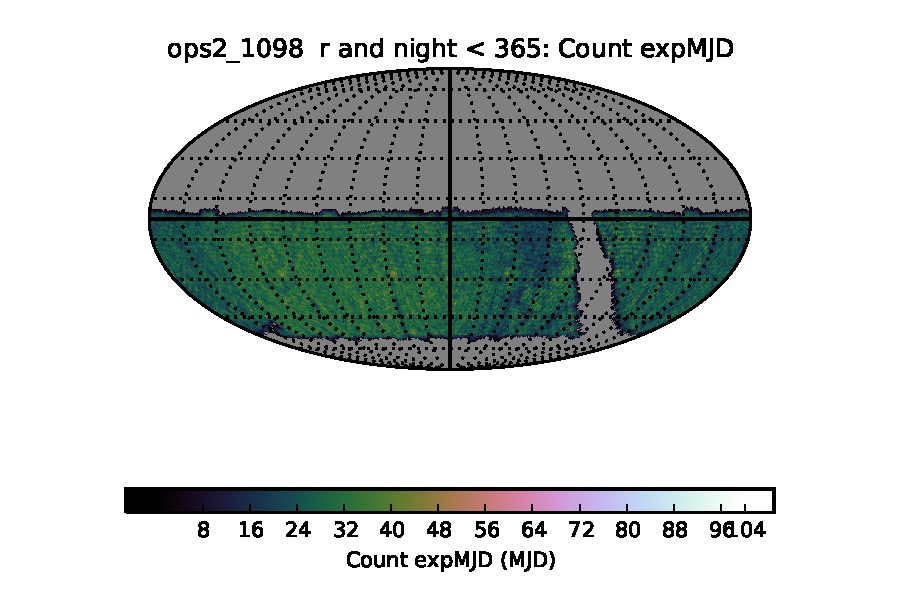
\includegraphics[width=2.3in]{figs/ops2_1098_Count_expMJD_r_and_night_lt_365_HEAL_SkyMap.pdf}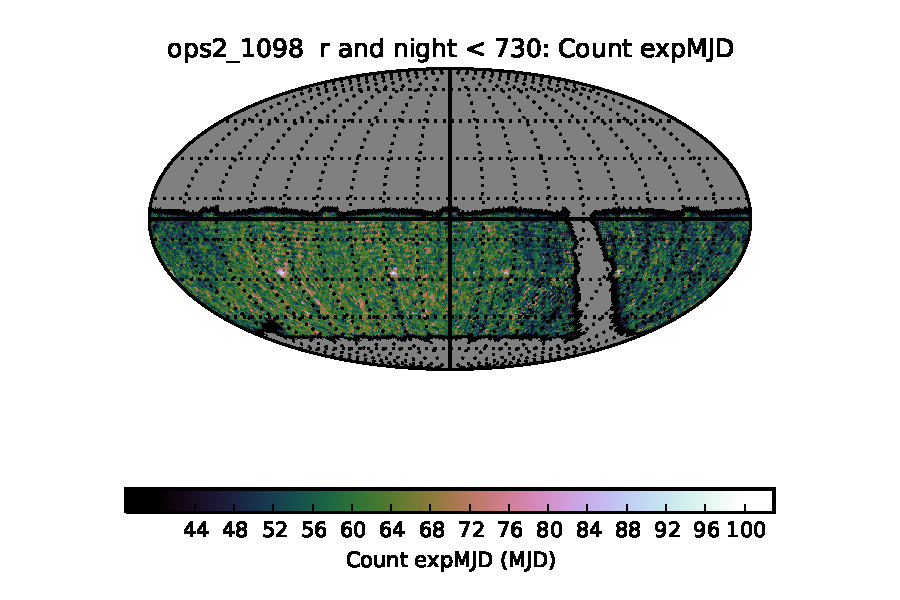
\includegraphics[width=2.3in]{figs/ops2_1098_Count_expMJD_r_and_night_lt_730_HEAL_SkyMap.pdf}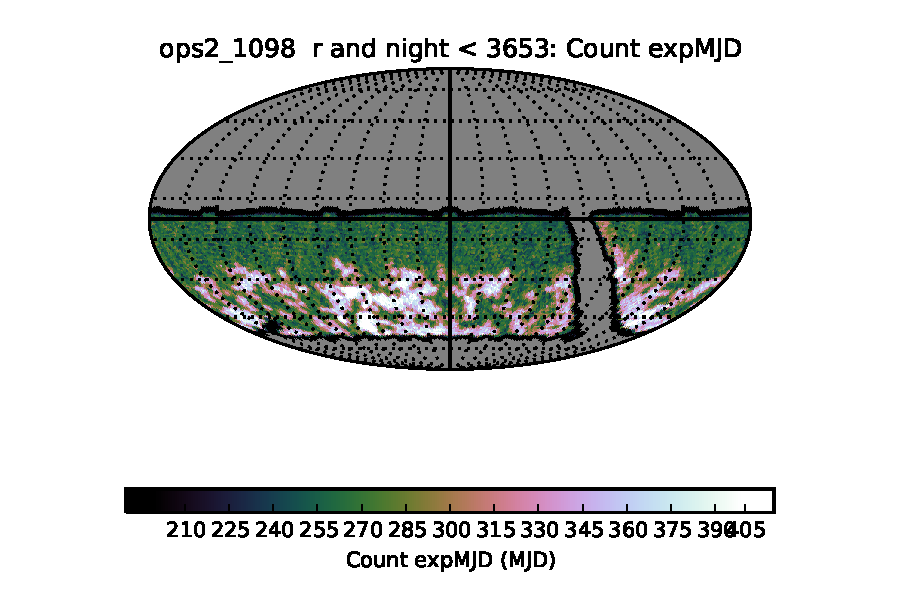
\includegraphics[width=2.3in]{figs/ops2_1098_Count_expMJD_r_and_night_lt_3653_HEAL_SkyMap.pdf} \\
  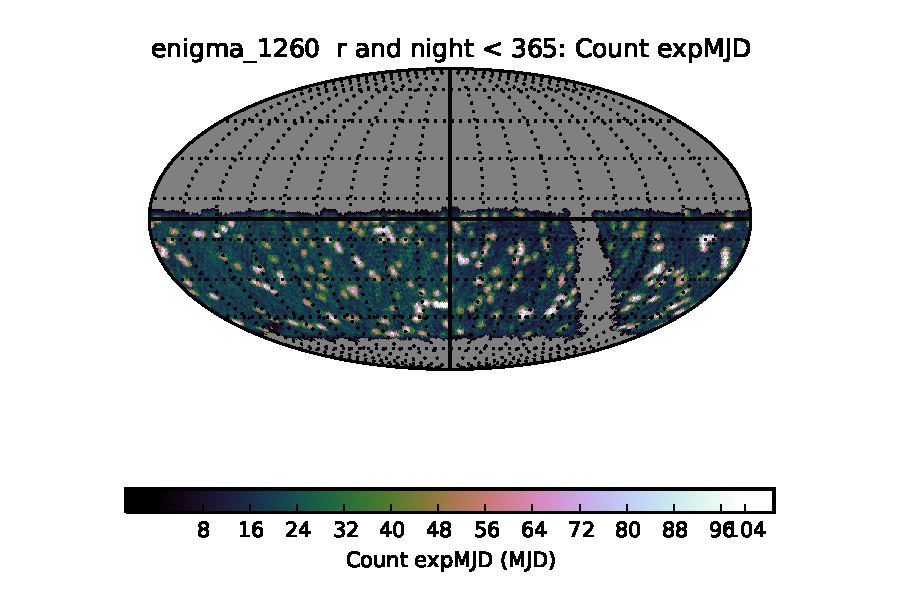
\includegraphics[width=2.3in]{figs/enigma_1260_Count_expMJD_r_and_night_lt_365_HEAL_SkyMap.pdf}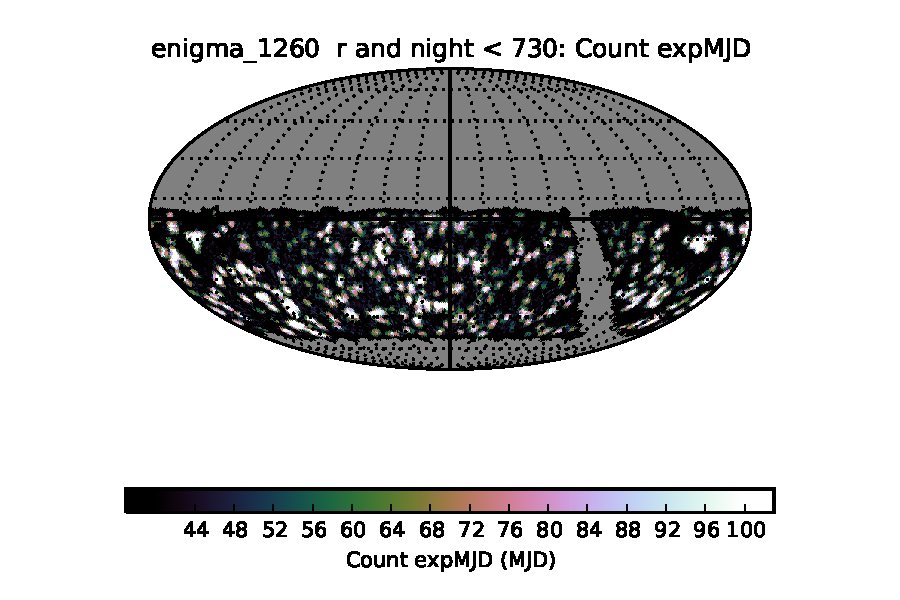
\includegraphics[width=2.3in]{figs/enigma_1260_Count_expMJD_r_and_night_lt_730_HEAL_SkyMap.pdf}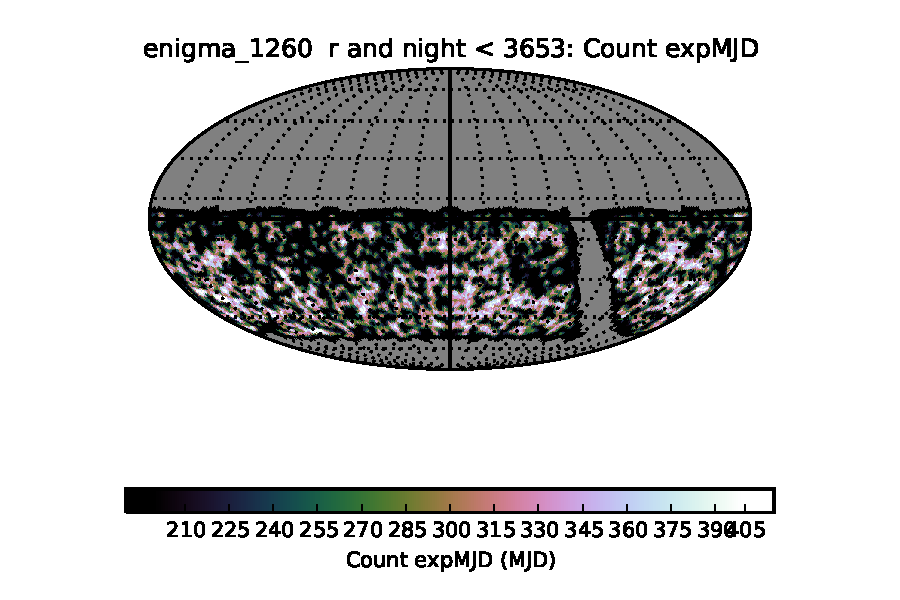
\includegraphics[width=2.3in]{figs/enigma_1260_Count_expMJD_r_and_night_lt_3653_HEAL_SkyMap.pdf}
  \caption{Example of a regular uniform survey (top) and a rolling cadence survey (bottom) after 1, 2, and 10 years in the $r$ filter.  For the regular survey, the number of visits for any part of the sky is relatively constant throughout the survey.  For the rolling cadence simulation, there are regions with many more exposures in year one which then fade in year two as other parts of the sky are emphasized.\label{fig:rollingcadence}}
\end{figure}

% --------------------------------------------------------------------
% --------------------------------------------------------------------
\subsection{ Supernovae and Rolling Cadence}
\label{sec:rolling:supernovae}

\noindent{\it Author Name(s)} % (Writing team)

Supernovae as a science topic are addressed elsewhere.
In this section, the demands of SN are used to directly constrain or
orient the rolling cadence development.

Pending more quantitative guidance, the SN objective for rolling cadence is to obtain multicolor time series significantly longer than the typical SN duration, with a cadence significantly faster than uniform.  As an example we discuss the option of a rolling cadence with the regular distribution of filters.

As a simple example, consider improving the cadence by a factor of 2 or 3.  Is we accept that some regions of the sky will be enhanced every year, and that uniform sky coverage will only arrive at the end of 10 years, then we could use, e.g., 10\% of the total epochs in a single roll.  If the enhancement is 2$\times$, each roll would last for $\simeq$ 6 months, with high efficiency for capture of complete SN events.  If the enhancement is 4$\times$, each roll would last for 2 months, with lower efficiency.

If it is important to achieve survey uniformity after 3 years, the available visits for each roll would be reduced also.  With a 2$\times$ enhancement of epoch frequency, a roll would last 2 months.

Some leverage would be gained by using more than 10\% of the available visits for a single roll.  However, this begins to impact the sampling of slow variables reduce schedule flexibility and robustness, and should be approached with caution.

From these examples, it appears that a 2$\times$ enhancement with uniformity closure after 10 years is relatively feasible and promising.  Much higher gains, or more rapid closure, require additional compromises.

% --------------------------------------------------------------------

\subsection{ Fast Transients and Rolling Cadence}
\label{sec:rolling:transients}

\noindent{\it Author Name(s)} % (Writing team)

Fast transients as a science topic are addressed elsewhere. In this section, the demands of fast transients are used to directly constrain or
orient the rolling cadence development.

By ``fast transients'', we are referring to events that are sufficiently fast that they are not addressed by the rolling cadence designed for SN observations, and slow enough that they are not covered in ``deep drilling'' type mini-surveys.  For higher tempo rolls, it is quite difficult to obtain full color data, because of the constraints on filter selection.  For this example, we will examine a rolling cadence utilizing only the {\it r} and {\it i} filters, as they are used for most visits. They are close in wavelength, and we assume that sufficient color information will be obtained by the ``background'' uniform survey that continues during a roll.

Again using 10\% of the available visits from the full 10 year survey for a single roll, we find that there would be enough epochs for each roll to acquire 1 visit per day for 21 consecutive days, giving an enhancement of 10$\times$.

Alternatively, the same epochs could be used to observe a target every 20 minutes for 12 hours during a single night (here it is assumed that visit pairs are not required, doubling the available epochs) for an enhancement of 300$\times$.

Several different possible redeployments of portions of a uniform survey have been described, each using 10\% of available time.  Of course it is possible in principal to implement multiple options, sequentially or maybe in parallel in some cases. This may pose considerable challenges to the scheduling strategy design by introducing incompatible boundary conditions.

While rolling cadences are powerful, they have limitations.  For example, sampling events that last longer than $\simeq$1 day and less than $\simeq$ 1 week have the obvious problem of diurnal availability.  In this example, intermediate cadences could be implemented in the circumpolar region, where diurnal access is much extended.  This is an example of a case in which a mini-survey of a limited number of regions could be considered as an alternative to a rolling cadence applied to the entire main survey.

% --------------------------------------------------------------------

\subsection{ Constraints, Trades and Compromises for Rolling Cadences}
\label{sec:rolling:trades}

While rolling cadences offer some attractive benefits, it is important to realize that rolling cadences are very highly constrained, and that they do bring disadvantages and compromises.

There are strong arguments against beginning a rolling cadence in the first, or even the second year of the survey.  Early in the survey, it is important to obtain for each field/filter combination, an adequate number of good quality photometric images, and at least one image in excellent seeing, to support closure of photometry reductions and to support generation of template images.

Since major science goals require a significant degree of survey homogeneity, it may be advisable to implement a strategy that brings the survey to nominal uniform depth at several times, e.g. after 3 or 5 years.  This would strongly constrain rolling cadences.

Some science objectives favor certain distributions of visits.  For astrometry, visits early and late in the survey and at large parallax factors, are beneficial.  Slow variables may benefit from uniform spacing.  Rolling cadences might impact these constraints either favorably or unfavorably.

Many objectives are served by randomization of observing conditions for each field.  Some rolling cadences could tend to reduce this randomization, for example by acquiring a large number of observations during a meteorologically favorable or unfavorable season, or during a period of instrument performance variance.

Dithering does not work gracefully with a rolling cadence, reducing temporal coverage at the boundaries of the selected sky region.  This is negligible for small dithers, but important for large dithers, which are under consideration.

These cautions illustrate that evaluation of rolling cadences must be based on the full range of schedule performance metrics, and not just those targeted by rolling cadence development.

\subsection{ Directions for Future Work with Rolling Cadences}
\label{sec:rolling:directions}

While preliminary experiments with rolling cadences have been carried out with OpSim, these experiments have signficant deficiencies, and are not suited for in-depth study as of this writing.  Progress in rolling cadence simulations is expected no sooner than mid to late-2016. Preparatory to that, analysis of cadences described above can guide development of objectives for enhancement by rolling cadence.  

Rolling cadences will be required to pass the same metrics as an other, and general requirements such as sky area, depth and visit count must be met.  Of particular interest will be metrics that clearly distinguish the gains available with rolling cadences - that is, metrics that measure schedule performance for variable targets, and especially those with strong sampling requirements, or more rapid variablity.

The following metrics, based on similar metrics developed for particular science objectives, may be useful in tuning rolling cadence performance. 

\begin{enumerate}
\item Observation Pairs histograms.  Visit pairs are simple and easy to quantify.  A pair of visits in the same filter describe a brightness change and constrain the rate of change. A visit pair in different filters (probably not coeval) constrain a color.  These metrics will describe how rapidly LSST can detect a change in the source fluxes. They will be useful for such science as early discovery of SNe, and identification of interesting galactic microlensing events.

\item Observation Triplets histograms. Similar to Pairs, but with closely spaced triplets allowing detection and confirmation of transient events (as described in http://arxiv.org/pdf/1508.03175v2.pdf).

\item Period determination metric.  Compute a measure of the period determination accuracy after a given time interval, as a function of period. A complete analysis would allow use of real light curves for various object types with realistic brightness distributions.  A simpler approach would use a single example light curve and a fixed measurement error value. A simplest approach would be based on the samping function and its power spectrum (as described in http://arxiv.org/pdf/1508.03175v2.pdf).  This metric group would rate simulation performance for period determination of periodic variables - mostly stars.

\item Sampling of SNe light curves.  The most complete metric would count the number of SNe (of various types) light curves that would be well sampled (according to defined criteria), based on analysis of realistic simulated data.  A simpler metric would be based on estimated sampling requirements and cadence without considering brightness. The latter could be used initially, pending replacement (or calibration) with more extensive simulations.

\item Time series count. For any transient or irregular variable, the optimum observational data will require multiple time and color samples within the duration of the event. Since the category of transients may include discoveries, it is not possible to exhaustively specify the source characteristics. A time series can be defined to consist of a series of samples, over some total duration T, with sampling interval t to tolerance d. The count of time series depends on the total duration, the number of samples, as well as the filter selection, so the challenge is how to visualize this information, and how to extract useful characteristic summary measures of performance.  This type of data can be valuable for identification and study of rapid phenomena such as stellar flares, binary mass transfer events, and exoplanet transits, and for slower events such as AGN reverberation mapping.

\end{enumerate}

% ====================================================================

\navigationbar

% ====================================================================
% commands for stand-alone printing
% \bibliographystyle{apj}
% \bibliography{references}
% \end{document}
% ====================================================================


% --------------------------------------------------------------------


% --------------------------------------------------------------------

% --------------------------------------------------------------------

\chapter[Cosmology]{Keeping It Even: Accurate Cosmological Measurements on the Largest Scales}
\def\chpname{cosmo}\label{chp:\chpname}

\noindent {\it
Eric Gawiser, Peter Kurczynski, Phil Marshall, Ohad Shemmer, Timo Anguita and others to follow
}

% --------------------------------------------------------------------

\section{Introduction}
\label{sec:\chpname:intro}

% Introduce, with a very broad brush, this chapter's science projects,
% and why it makes sense for them to be considered together.

Cosmology is one of the key science themes for which LSST was designed. Our goal is to measure cosmological parameters, such as the equation of state of dark energy, or departures from General Relativity, with sufficient accuracy to distinguish one model from another, and hence drive our theoretical understanding of how the universe works, as a whole. To do this will necessarily involve a variety of different measurements, that can act as cross-checks of each other, and break parameter degeneracies in any single one.

The  Dark Energy Science Collaboration (DESC) has identified five
different cosmological probes enabled by the LSST: weak lensing (WL),
large scale structure (LSS), type Ia supernovae (SN), strong lensing
(SL), and clusters of galaxies (CL). In all cases, the primary concern
is residual systematic error: the shapes and photometric redshifts of
galaxies, and the properties of supernova and lensed quasar light
curves, will all need to be measured with extraordinary accuracy in order for LSST's high statistical power to be properly harnessed. This accuracy will come from the abundance and heterogeneity of the individual measurements made, and the degree to which they can be modeled and understood. This latter point implies a need for uniformity in the survey, which enables powerful simplifying assumptions to be made when calibrating on the largest, cosmologically most important scales. The need for heterogeneity also implies  uniformity, in the sense that the nuisance parameters that describe the systematic effects need to be sampled over as wide a range as possible (examples include the need to sample a wide range of roll angles to minimize shape error, and observing conditions to understand photometric errors due to the changing atmosphere).

In this chapter we look at some of the key measurements planned by the Dark Energy Science Collaboration, and how they depend on the Observing Strategy.

% Anticipate the results of the chapter: summarize the results of a
% number of investigative sections, where there will be one on each
% science case.

%---------------------------------------------------------------------

% ====================================================================
%+
% SECTION NAME:
%    dithering.tex
%
% CHAPTER:
%    cosmology.tex
%
% ELEVATOR PITCH:
%    Large Scale Structure, Weak Lensing, and Clusters all require
% survey uniformity in the static 10-year survey.  A key contributor to 
%this is the pattern of dithers adopted.  
%
% COMMENTS:
%
%
% BUGS:
%
%
% AUTHORS:
%   Eric Gawiser (@egawiser)
%-
% ====================================================================
\clearpage
\section{Dithering Patterns and Timescales}
\def\secname{dithering}\label{sec:\secname}

\noindent{\it Humna Awan, Eric Gawiser, Peter Kurczynski, Lynne Jones} % (Writing team)

% This individual section will need to describe the particular
% discoveries and measurements that are being targeted in this section's
% science case. It will be helpful to think of a ``science case" as a
% ``science project" that the authors {\it actually plan to do}. Then,
% the sections can follow the tried and tested format of an observing
% proposal: a brief description of the investigation, with references,
% followed by a technical feasibility piece. This latter part will need
% to be quantified using the MAF framework, via a set of metrics that
% need to be computed for any given observing strategy to quantify its
% impact on the described science case. Ideally, these metrics would be
% combined in a well-motivated figure of merit. The section can conclude
% with a discussion of any risks that have been identified, and how
% these could be mitigated.

% A short preamble goes here. What's the context for this science
% project? Where does it fit in the big picture?

Three of the key cosmology probes available with LSST represent ``static science'' insensitive to time-domain concerns.  These are Weak Lensing, Large-Scale Structure, and Galaxy Clusters.  Nonetheless, due to the need to track and correct for the survey ``window function'' in all of these probes, cosmology with LSST will benefit greatly from achieving survey depth as uniform as possible over the WFD area.  OpSim tiles the sky in hexagons inscribed within the nearly-circular LSST field-of-view.  It has been shown in \citet{CarrollEtal2014} that the default LSST survey strategy implemented in OpSim runs leads to a strongly non-uniform ``honeycomb'' pattern due to overlapping regions on the edges of these hexagons receiving double the observing time.  A pattern of large dithers proves sufficient to greatly reduce these overlaps, leading to an increase in median survey depth in each filter of 0.08 magnitudes.  

In this section, we report results from an investigation by Awan et al. (in preparation) of several geometrical patterns for dithers performed on timescales varying from once per observing season to once per night to every visit.  

\todo{EG}{Flesh out WL, LSS, and Clusters dependence on survey uniformity to make this section more clearly science-driven.}  

% --------------------------------------------------------------------

\subsection{Dithering Patterns and Timescales}
\label{sec:\secname:strategies}


% --------------------------------------------------------------------

\subsection{Metrics}
\label{sec:\secname:metrics}

% Quantifying the response via MAF metrics: definition of the metrics,
% and any derived overall figure of merit.

Our primary metric is total uncertainty in the derived window function over relevant angular scales, modeled via variations in the angular power spectrum of fake galaxy fluctuations between $gri$ bands.  
Intermediate metrics include the number of galaxies in 
each pixel, fluctuations in this number, total power in the angular power spectrum of a skymap of those fluctuations, and residual power that angular power spectrum after subtracting a smooth fit to it.  



% --------------------------------------------------------------------

\subsection{OpSim Analysis}
\label{sec:\secname:analysis}

% OpSim analysis: how good would the default observing strategy be, at
% the time of writing for this science project?

In this section we present our ongoing \OpSim / MAF
analysis, as we try to
answer the question ``what dithering strategies produce acceptable variations in survey uniformity, and which appears optimal?''

%We used the
%\simsMAFcontrib{SeasonStacker}{mafContrib/seasonStacker.py} to work
%with seasons.

%We used \texttt{ops2\_1075} for most of our tests, but we need to now
%re-run on \opsimdbref{db:enigma}, and others from \autoref{chp:cadence2015}.


%\citeauthor{LiaoEtal2015}). These sky maps show that, over the main

%\autoref{tab:lenstimedelays:results} shows the global (i.e. al-sky)


%--------------------------------------------------------------------

\subsection{Results}
\label{sec:\secname:results}

%%%%%%%%%%%%%%%%%%%%%%%%%%%%%%%%%%%
\begin{figure*}[!ht]
  \capstart
  \begin{minipage}[b]{\linewidth}
    \begin{minipage}[b]{0.32\linewidth}
      \centering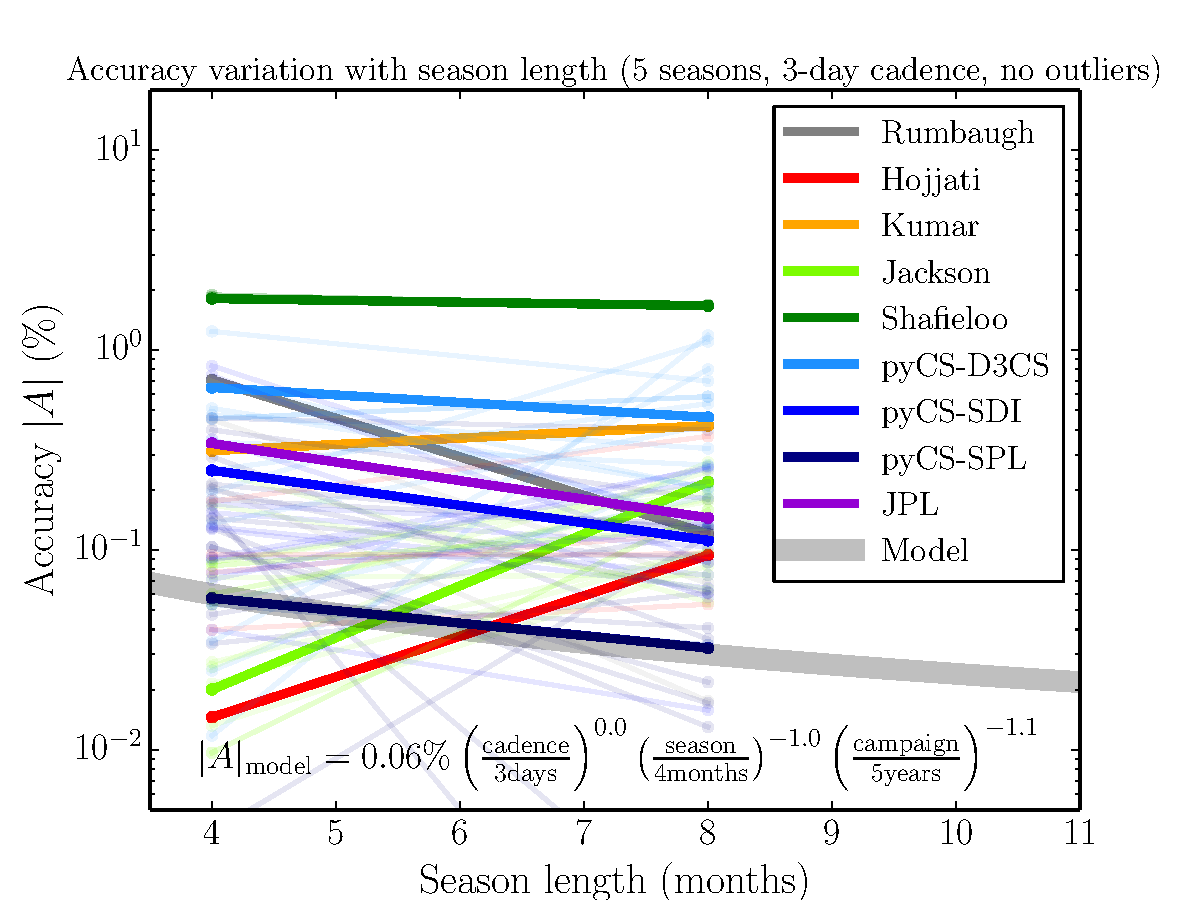
\includegraphics[width=\linewidth]{figs/Accuracy_season_nca.pdf}
    \end{minipage} \hfill
    \begin{minipage}[b]{0.32\linewidth}
      \centering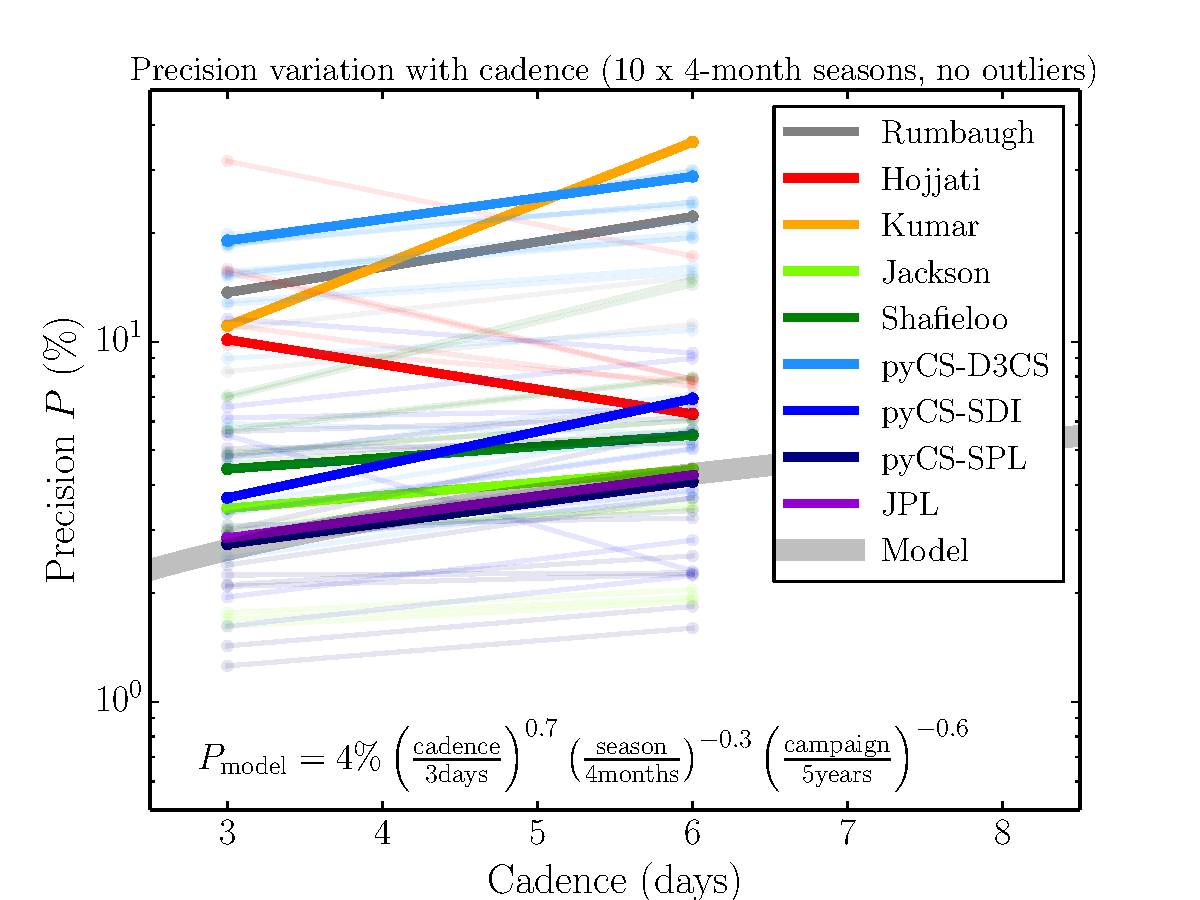
\includegraphics[width=\linewidth]{figs/Precision_cadence_nca.pdf}
    \end{minipage} \hfill
    \begin{minipage}[b]{0.32\linewidth}
      \centering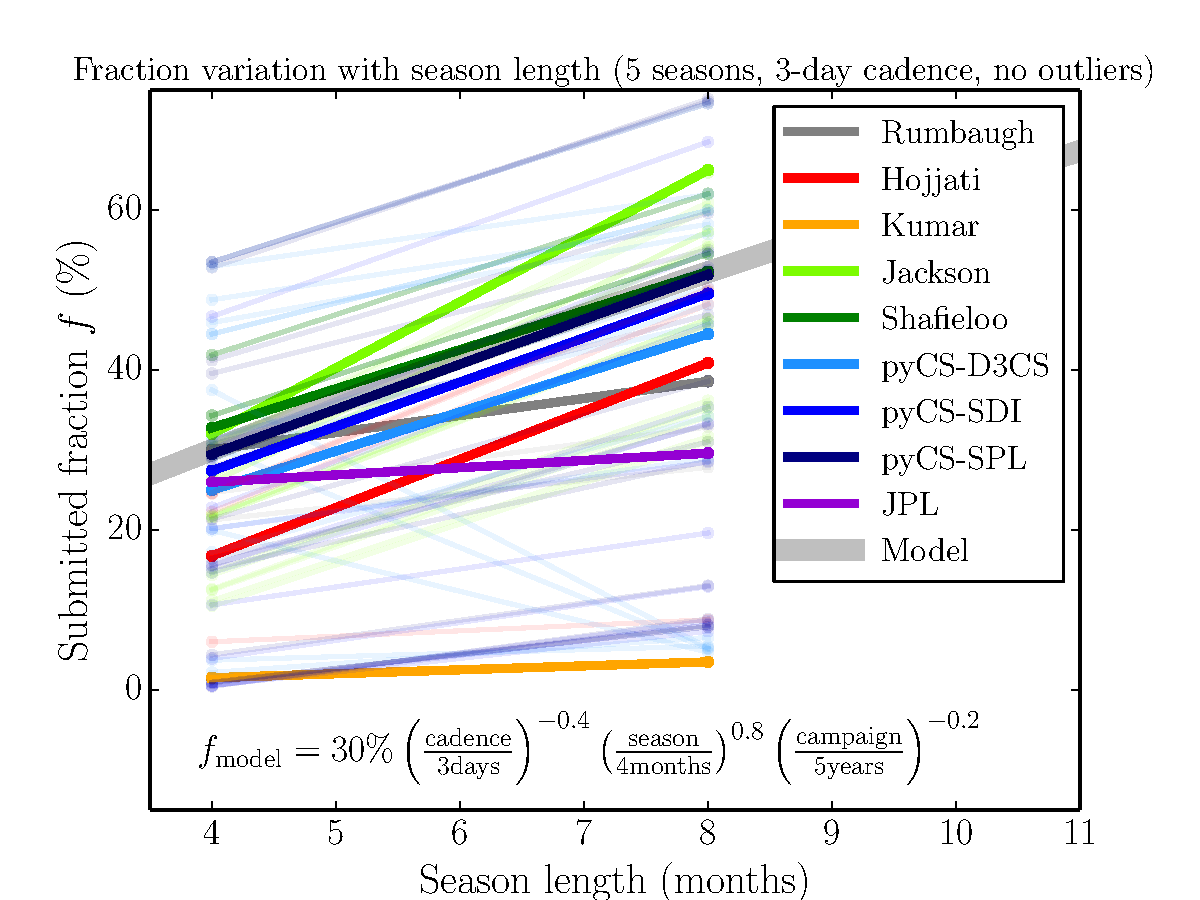
\includegraphics[width=\linewidth]{figs/Fraction_season_nca.pdf}
    \end{minipage}
  \end{minipage}
\caption{Examples of changes in accuracy $A$ (left), precision $P$ (center) and success fraction $f$ (right) with schedule properties, as seen in the different TDC submissions. The gray
approximate power law model was derived by visual inspection of the
pyCS-SPL results; the signs of the indices were pre-determined according to our expectations. Reproduced from \citet{LiaoEtal2015}.}
\label{fig:tdcresults}
\end{figure*}
%%%%%%%%%%%%%%%%%%%%%%%%%%%%%%%%%%%


\todo{EG}{Improve figures to originals rather than screen-captures.}

\todo{EG}{Input fuller results and text from Awan et al. draft.}  

%---------------------------------------------------------------------

\subsection{Discussion}
\label{sec:\secname:discussion}



\navigationbar

% ====================================================================
  

% --------------------------------------------------------------------

% ====================================================================
%+
% SECTION NAME:
%    lenstimedelays.tex
%
% CHAPTER:
%    cosmology.tex
%
% ELEVATOR PITCH:
%    Lensed quasars and supernovae provide distance measurements for
%    cosmology. They are a few days to a few weeks in length. To
%    measure them well we need long campaigns (>~3 years) with high
%    night-to-night cadence (better than the standard 5 days if
%    possible, especially as combining all filters might be difficult.)
%
% COMMENTS:
%
%
% BUGS:
%
%
% AUTHORS:
%   Phil Marshall (@drphilmarshall)
%-
% ====================================================================

\section{ Strong Gravitational Lens Time Delays }
\label{sec:lenstimedelays}

\noindent{\it Phil Marshall} % (Writing team)

% This individual section will need to describe the particular
% discoveries and measurements that are being targeted in this section's
% science case. It will be helpful to think of a ``science case" as a
% ``science project" that the authors {\it actually plan to do}. Then,
% the sections can follow the tried and tested format of an observing
% proposal: a brief description of the investigation, with references,
% followed by a technical feasibility piece. This latter part will need
% to be quantified using the MAF framework, via a set of metrics that
% need to be computed for any given observing strategy to quantify its
% impact on the described science case. Ideally, these metrics would be
% combined in a well-motivated figure of merit. The section can conclude
% with a discussion of any risks that have been identified, and how
% these could be mitigated.

A short preamble goes here. What's the context for this science
project? Where does it fit in the big picture?

% --------------------------------------------------------------------

\subsection{Target measurements and discoveries}
\label{sec:lenstimedelays:targets}

Describe the discoveries and measurements you want to make.

Now, describe their response to the observing strategy. Qualitatively,
how will the science project be affected by the observing schedule and
conditions? In broad terms, how would we expect the observing strategy
to be optimized for this science?


% --------------------------------------------------------------------

\subsection{Metrics}
\label{sec:lenstimedelays:metrics}

Quantifying the response via MAF metrics: definition of the metrics,
and any derived overall figure of merit.


% --------------------------------------------------------------------

\subsection{OpSim Analysis}
\label{sec:lenstimedelays:analysis}

OpSim analysis: how good would the default observing strategy be, at
the time of writing for this science project?


% --------------------------------------------------------------------

\subsection{Discussion}
\label{sec:lenstimedelays:discussion}

Discussion: what risks have been identified? What suggestions could be
made to improve this science project's figure of merit, and mitigate
the identified risks?


% ====================================================================


% --------------------------------------------------------------------

% ====================================================================
%+
%
% SECTION NAME:
%    \secname.tex
%
% CHAPTER:
%    ???.tex
%
%
% COMMENTS:
%
%
% BUGS:
%
%
% AUTHORS:
%   Ohad Shemmer (@ohadshemmer), Timo Anguita (@tanguita), Niel Brandt, Gordon Richards, Scott Anderson(?),
%   Phil Marshall(?) (@drphilmarshall) 
%-
% ====================================================================

\section{AGN Science}
\def\secname{agn}\label{sec:\secname}

\noindent{\it Ohad Shemmer, Timo Anguita, Niel Brandt, Gordon Richards, Scott Anderson(?), Phil Marshall(?)}

% This section discusses the potential effects of the LSST observing strategy on AGN science. In short, there appears to be
% a consensus among the AGN and galaxies communities that AGN science will benefit from the most uniform cadence in
% terms of even sampling for each band and uniform sky coverage. It is also expected that any reasonable
% perturbation to the nominal LSST observing strategy will have mostly minor effects on AGN science. This section attempts
% to identify all the areas of AGN science that may be affected by the observing strategy and to point out the metrics that
% can be used to quantify any potential effect. Since the total number of metrics that must be quantified is quite large, and
% the effects are likely small in most cases, the goal of this section is to identify potential ``killers'' that may undermine
% key AGN research areas. For example, certain perturbations may reduce significantly the number of ``interesting'' AGNs,
% such as $z>6$ quasars, lensed quasars, or transient AGNs. Another example is photometric reverberation mapping
% which is one of LSST's greatest advantages for AGN research but is also very sensitive to the cadence; care must
% be taken to ensure that the observing strategy does not undermine the ability to make the best use of this method.

\subsection{AGN Selection and Census}
\label{sec:\secname:selection}

\noindent About $10^7 - 10^8$ AGNs will be selected in the main LSST survey using a combination of criteria, split
broadly into four categories: colors, astrometry, variability, and multiwavelength matching with other surveys.
The LSST observing strategy will affect mostly the first three of these categories.

{\bf Colors:}~The LSST observing strategy will determine the depth in each band, as a function of position on the sky, and will thus affect
the color selection of AGNs. This will eventually determine the AGN $L-z$ distribution and, in particular, may affect the identification
of quasars at $z\gtsim 6$ if, for example, $Y$-band exposures will not be sufficiently deep.

{\bf Variability:} AGNs can be effectively distinguished from (variable) stars, and from quiescent galaxies, by exhibiting certain characteristic variability patterns (e.g., Butler \& Bloom 2011). Non-uniform sampling may ``contaminate'' the variability signal of AGN candidates.

{\bf Astrometry:} AGNs will be selected among sources having zero proper motion, within the uncertainties. The LSST cadence
may affect the level of this uncertainty in each band, and may therefore affect the ability to identify (mostly fainter) AGNs.
%
Differential chromatic refraction (DCR), making use of the astrometric offset a source with emission lines has with respect to
a source with a featureless power-law spectrum, can help in the selection of AGNs and in confirming their photometric redshifts (Kaczmarczik~et~al.~2009). The DCR effect is more pronounced at higher airmasses. AGN selection and photometric redshift confirmation may be affected since the LSST cadence will affect the airmass distribution, in each band, for each AGN candidate.

\subsection{AGN Clustering}
\label{sec:\secname:clustering}

\noindent Measurements of the spatial clustering of AGNs with respect to those of quiescent galaxies can provide clues as to how galaxies
form inside their dark-matter halos and what causes the growth of their supermassive black holes (SMBHs). The impressive inventory 
of LSST AGNs will enable the clustering, and thus the host galaxy halo mass, to be determined over the widest range ranges of cosmic
epoch and accretion power.
%
The LSST cadence will not only affect the overall AGN census and its $L-z$ distribution, but also the
depth in each band as a function of sky position that can directly affect the clustering signal.

\subsection{AGNs and the Time Domain}
\label{sec:\secname:time}

{\bf AGN Variability:} A variety of AGN variability studies will be enabled by LSST. These are intended to probe the physical properties of the unresolved inner regions of the central engine. Relations will be sought between variability amplitude and timescale vs. $L$, $z$, $\lambda_{\rm eff}$, color, multiwavelength and spectroscopic properties, if available. The LSST sampling is expected to provide high-quality power spectral density functions for a large number of AGNs; these can be used to constrain the SMBH mass and accretion rate/mode. Furthermore, LSST AGNs exhibiting excess variability over that expected from their luminosities will be further scrutinized as candidates for lensed systems having unresolved images with the excess (extrinsic) variability being attributed mainly to microlensing.

Photometric reverberation mapping (PRM), measuring the time-delayed response of either the flux of the broad emission line region (BELR) lines to the flux of the AGN continuum or between the continuum flux in one (longer wavelength) band to the continuum flux in another (band with shorter wavelength), will be one of the cornerstones of AGN research in the LSST era
(e.g., Chelouche 2013; Chelouche \& Zucker 2013; Chelouche~et~al.~2014). For example, LSST is expected to deliver BELR line-continuum time delays in $\sim10^5-10^6$ sources, which is unprecedented when compared to $\sim50-100$ such measurements conducted via the traditional, yet much more expensive (per source) spectroscopic method. Sources in the deep-drilling fields (DDFs) will benefit from the highest quality PRM
time-delay measurements given the factor of $\sim10$ denser sampling. The PRM measurements will probe the size and structure of the accretion disk and BELR, in a statistical sense, and may provide improved SMBH mass estimates for sources that have at least single-epoch spectra.

The PRM method is very sensitive to the sampling in each band, therefore the ability to derive reliable time delays can be affected significantly
by the LSST cadence. The best results will be obtained by having the most uniform sampling equally for each band. Additionally, there is
a trade-off between the number of DDFs and the number of time delays that PRM can obtain (Chelouche~et~al.~2014). For example,
an increase in the number of DDFs, with similarly dense sampling in each field, can yield a proportionately larger number of high-quality time delays,
down to lower luminosities, but at the expense of far fewer time delays (of relatively high luminosity sources) in the main survey.

{\bf Time Delays in Gravitationally Lensed Quasars:} This aspect is discussed in detail in the lenstimedelays.tex section.

{\bf AGN Size and Structure with Microlensing:} Microlensing due to stars projected on top of individual lensed quasar images produce additional magnification. Using the fact that the Einstein radii of stars in lensing galaxies closely match the scales of different emission regions in high-redshift AGNs (micro-arcseconds), analyzing microlensing induced flux variations statistically on individual systems allows us to measure ``sizes'' of AGN regions.
%
Assuming a thermal profile for accretion disks, sizes in different emission wavelengths will be probed and as such, constraints on the slope of this thermal profile. Given the sheer number of lensed systems that LSST is expected to discover ($\sim8000$), this will allow us to stack systems for better constraints and hopefully determine the evolution of the size and profile. Due to the typical relative velocities of lenses, microlenses, observers (Earth) and source AGN, the microlensing variation timescales are between months to a few decades.

The quasar microlensing optical depth is $\sim1$, so every lensed quasar should be affected by microlensing at any given point in time. However, measurable variability can occur on longer timescales. Mosquera~et~al.~(2011) did a study using all known lensed quasars. They found the median timescale between high magnification events (Einstein crossing time scales) in the observed $I$-band is of the order of $\sim20$~yr (with a distribution between 10 and 40~yr). However, the source crossing time (duration of a high magnification event) is $\sim7.3$~months (with a distribution tail up to 3~yr). This basically means that out of all the lensed quasar {\em images} (microlensing between images is completely uncorrelated) about half of them will be quiescent during the 10~yr baseline of LSST. However, since the typical number of lensed images is either two or four, it means that, statistically, in every system, one (for doubles) or two (for quads) high magnification events should be observed in 10~yr of LSST monitoring.

Note that, the important cadence parameter is the source crossing time, as it is the length of the event to be as uniformly sampled as possible. The 7.3 months crossing time is the median for the observed $i$-band, but this time would be significantly shorter for bluer bands: for a thermal profile with slope $\alpha: R_\lambda \propto \lambda^\alpha$ implies source crossing time $t_{\rm s} \propto \lambda^\alpha \rightarrow t_u=t_i \times (\lambda_{\rm u} / \lambda_{\rm i})^{\alpha}$. For a Shakura-Sunyaev slope of $\alpha=0.75$ this would correspond to $7.3 \times (3600/7500)^{3/4}$ months $= 4.2$ months in the $u$-band.

In terms of the cadence, at least three evenly sampled data points per band within 2 to 3 months would be preferred to be able to map the constraining high magnification event(?). Hopefully uniformly spaced. Very tight cadence (e.g., DDFs) would increase the constraints significantly. However, since lensed quasars are not that common, this smaller area would mean only a few ($\sim80$?) suitable systems monitored in the DDFs.
%
Regarding the season length, the ``months'' timescale of high magnification events very likely means that we can/will miss high magnification events in the season gaps, at least in the bluer bands.
%
Killer: observations spread on timescales larger than 3 months(??). This would likely miss the high magnification events. In those cases we could perhaps consider close consecutive photometric bands as equivalent accretion disk regions, however this would mean weaker constraints on the thermal profile.
%
Important Note: all this science needs to be done on lensed quasars with measured or very short time delays to remove the intrinsic variability signal.

{\bf Microlensing Aided Reverberation Mapping:} Given that microlensing mostly affects continuum emission rather than BELR line emission, microlensing may enable disentangling the BELR line $+$ continuum emission in single photometric bands, allowing the use of single broad band PRM measurements (Sluse \& Tewes 2014). As with the two-band PRM method discussed above, the denser (and the longer) the sampling, the more accurate are the constraints that can be obtained for the time delays.

{\bf Transient AGN and TDEs:} This aspect is discussed in detail in the variablesandtransients.tex section(?)

% --------------------------------------------------------------------

\subsection{Metrics}
\label{sec:\secname:metrics}

% Quantifying the main impacts on AGN science via MAF metrics, including the effects
% of additional cadence facto,rs such as the number of DDFs
% and MC fields, or different dithering patterns,: definition of the metrics,
% and any derived overall figure of merit.

{\bf Selection:} Need to compute the mean $Y$ band magnitude across the sky for the nominal
OpSim. Compare this magnitude to the one required for identifying $\geq1000$ quasars
at $z\geq6$.

{\bf PRM:} Need to compute the average and the dispersion in the number of visits, per band, across the sky
for the nominal OpSim (during the entire survey). By running RPM simulations, identify the 1) minimum number of visits (in any band) that can yield any lag estimates with high confidence, and 2) the largest difference in visits between two
different bands that can yield any lag estimates with high confidence. Repeat these simulations by doubling the nominal number of DDFs.

{\bf Microlensing:} Need to compute the dispersion in the time gap between visits in the same band, across the sky,
in order to assess the number of microlensing events that can be monitored.

% --------------------------------------------------------------------

\subsection{Discussion}
\label{sec:\secname:discussion}

% Discussion: what risks have been identified? What suggestions could be
% made to improve the figures of merit, and mitigate the identified risks?
% What ``tweaks'', if any, can be proposed to the nominal LSST observing strategy
% in order to help achieve key AGN science goals?

\navigationbar


% --------------------------------------------------------------------


% --------------------------------------------------------------------

% ====================================================================
%+
% SECTION:
%    supernovacosmology.tex
%
% CHAPTER:
%    cosmology.tex
%
% ELEVATOR PITCH:
%    SNIa cosmology, approach to evaluating dependence of science on cadence
%
% COMMENTS:
%
%
% BUGS:
%
%
% AUTHORS:
%    Phil Marshall (@drphilmarshall)  - put your name and GitHub username here!
%-
% ====================================================================

\section{Supernova Cosmology and Physics}
\def\secname{supernovae}\label{sec:\secname}
% \label{sec:cosmology, supernovae, classification, lenstimedelays, deepdrillingfields }

\noindent{\it Jeonghee Rho, Michelle Lochner, Rahul Biswas, Seth Digel} % (Writing team)

% This individual section will need to describe the particular
% discoveries and measurements that are being targeted in this section's
% science case. It will be helpful to think of a ``science case" as a
% ``science project" that the authors {\it actually plan to do}. Then,
% the sections can follow the tried and tested format of an observing
% proposal: a brief description of the investigation, with references,
% followed by a technical feasibility piece. This latter part will need
% to be quantified using the MAF framework, via a set of metrics that
% need to be computed for any given observing strategy to quantify its
% impact on the described science case. Ideally, these metrics would be
% combined in a well-motivated figure of merit. The section can conclude
% with a discussion of any risks that have been identified, and how
% these could be mitigated.

This section is concerned with the detection and characterization of supernovae (SNe)
over time with LSST and their various scientific applications.
The most important
application is the use of supernovae type Ia (SNIa) and potentially some core-collapse SN (like type IIP) to trace the recent expansion history of the universe,
and confront models of the physics driving the late time accelerated expansion
of the universe. 

This objective of SN cosmology follows (at least for SNIa) results from several
highly successful surveys; improvement in knowledge of cosmology could come from
substantially larger numbers of well-characterized SNe.
This
goal is not directly tied to the unprecedentedly large survey area of LSST.  
However, we shall argue that in practice, even this
goal would benefit from the spatial scale offered by the WFD
component of the LSST survey. 

On the other hand, the WFD aspect will make the LSST survey potentially the 
first to scan the very large area of the entire Southern sky for SNe. 
SNe that are detected and well characterized by LSST will
probe the isotropy of the universe.  Peculiar velocities of 
SNe will probe the growth of structure.  In addition, this large sample
will enable further
sharpening of our understanding of the properties of the SN population 
of different types. 
This last point is extremely important for SN cosmology goals:  The success of SNIa cosmology has always been based on the empirical model that intrinsic peak brightnesses are related to the certain observable characteristics of SNe. 
%While the spatial locations of the SNe are not important
The 
WFD SNIa sample will dramatically increase the size of the sample 
available to train such an empirical model, as well understand the probability of deviations and scatter from this model. Aside from issues like calibration 
which need to be addressed differently, a larger sample of such well measured SNe is probably the only way to address `systematics' due to deviations from the empirical
model. The anticipated sample can be thought of as consisting of two 
components:  the low-redshift sample which is more likely to be complete, and the higher-redshift sample that will be able to constrain evolution. 
% --------------------------------------------------------------------

\subsection{Target measurements and discoveries}
\label{sec:keyword:targets}

% Describe the discoveries and measurements you want to make.

SNe of different types are visible over time scales of about a few 
weeks (e.g., type Ia) to nearly a year (type IIP).  During the full ten-year
 survey, LSST will scan the entire southern sky repeatedly
 with a WFD cadence, and certain specific locations
of the sky called the Deep Drilling Fields (DDF) with special enhanced cadence. 

This spatio-temporal window should contain millions \todo{RB}{remember to check} of SNe, that will have apparent magnitudes brighter than the single exposure limiting magnitude of LSST.  However, the actual
 sequence of observations by LSST, defined by the series of field pointings as a
 function of time in filter bands (along with weather conditions), will
 determine the extent to which each SN can be detected and
 characterized well.  Characterization of the SNe is at the core of a
 number of science programs that use them as bright, abundant objects with empirically determined intrinsic brightnesses. For LSST, this goal entails (a) detection of SNe, (b) photometric typing of SNe, (c) estimating photometric redshifts of SNe (or identifying host galaxies 
 and obtaining their redshifts from photometry or follow-up spectroscopy),
(d) estimation of intrinsic brightnesses of the SNe, and finally (e) use of these data in addressing our science goals of cosmological inference, etc.
The efficacy of photometric typing, redshifts and estimation of intrinsic brightnesses are all
dependent on the amount of information available in the observed light curves of SNe. While these steps are not necessarily independent, it is useful to think of the requirements on some of these steps separately; it is not unlikely  that combinations of some of the steps would still be affected by similar requirements. 

{\emph{Our first objective is to detect such SNe}}, by which we mean
selecting SNe from among the transient sources detected by LSST.
% classify them as SNe (as opposed to an AGN, or an asteroid). 
In brief, this process 
consists of defining a set of image subtractions between a high-resolution
`template` image of a sky section, and a set of single exposures at
different times (usually of lower resolution) of the same region, after 
accounting for the different resolutions of images, and alignments. These sets of image subtractions associated
 with a single object will be used to detect the object as a transient and then
classify the transient as an SN. Clearly, detecting an SN depends on the number of such images recorded per object, the different filters used for those images, and the signal-to-noise ratios of the images. %One might expect that 
The efficiency of this step may be summarized as a threshold on the joint properties 
of an astrophysical candidate (apparent brightness, light curve characteristics, background) as well as observing conditions (astronomical seeing, etc.).  

{\emph{Our second objective is to photometrically classify different kinds of SNe.}} 
%{\bfseries Photometric SN classification}\\
Previously, only spectroscopically typed SNe have been used for cosmology. Photometric 
typing from light curves alone has only been used to select candidates for spectroscopic 
follow-up (see, e.g., \citet{Sako2008}). However, LSST will simply find far too many 
candidates for even a significant fraction of them to be followed up spectroscopically. In order to avoid 
discarding the majority of the SN dataset, we need to use techniques capable of 
determining cosmological parameters from a potentially contaminated photometric SN dataset.

Several techniques have been proposed recently to solve this problem. One 
approach involves applying stringent cuts to the photometric dataset to obtain a nearly pure sample 
of SNIa\citep{Bernstein2012,Campbell2013} and running the standard SNIa cosmology analysis 
with this sample. Another approach, BEAMS \citep{Kunz2007,Newling2011,Hlozek2012,Knights2013}, 
makes use of an entire dataset, coping with contamination by using a mixture model for the 
likelihood, thus allowing for multiple populations. Whatever the technique ultimately used for 
cosmological analysis, it will rely on accurate initial classifications of SN type and 
unbiased estimates for the probability of each type.

Current state-of-the-art photometric classification techniques rely on fitting empirically 
determined templates of SNe to light curves \citep{Jha2007,Guy2007,Sako2011}. However in 
recent years, new approaches have been developed in response to the 2010 `Supernova 
Photometric Classification Challenge' \citep{Kessler2010a}. Many of these use novel light curve 
parameterization and employ machine learning algorithms to perform the classification (see \citet{Kessler2010b} and references therein).

While many of these methods have been tested on standard sets of simulated data and (in some cases) 
on SDSS data, which technique (if any) is superior in all situations is unclear. For 
example, some techniques are dependent on the availability of reliable redshift information. 
%, while others  are less reliant on it. 
Some techniques may be more robust to non-representative datasets [Not sure what this means] than 
others, and how the techniques will respond to changes in cadence, filter sets, signal-to-noise, 
etc., is unclear.  

With this in mind, we propose the use of a multifaceted classification system which employs 
several different methods for extracting features from the light curves (e.g., fitting parametric 
functions or templates) and several different classification algorithms. This system is highly 
modular, allowing new approaches for direct comparison with existing  techniques to be added easily. This also allows direct analysis of different observing strategies, without requiring 
an initial choice of classification technique. 


{\emph{Our third objective is to characterize SNe in terms of empirical
    light curve models.}}

The ultimate goal of using SNe (type SNIa or SNIIP) for cosmology requires estimating the intrinsic brightnesses of the SN. The
first (and sometimes only, depending on the light curve model) step is
fitting the calibrated fluxes to a light curve model with a set of parameters.
According to the ansatz used in SN cosmology, the intrinsic brightness of
 SNe is largely determined by the parameters of the light curve model; 
 hence the uncertainties on the inferred parameters largely determine the
 uncertainties on the inferred peak intrinsic brightness or distance moduli of the SNe.

% Now, describe their response to the observing strategy. Qualitatively,
% how will the science project be affected by the observing schedule and
% conditions? 

% In broad terms, how would we expect the observing strategy
% to be optimized for this science?





% --------------------------------------------------------------------

\subsection{Metrics}
\label{sec:keyword:metrics}

Quantifying the response via MAF metrics: definition of the metrics,
and any derived overall figure of merit.
\label{sec:keyword:metrics}

\begin{center}
\begin{tabular}{| p{5cm} |p{10cm} |p{2cm}}
\hline Metric & Description & Status\\
\hline
SN discovery I  &  Identify the number of LSST data points and quality required & \\
SN light curve I & Generate SN light curves using OpSim output of baseline Cadence &\\
SN classification & Classify identified SNe into SN Ia, II, Ib, and Ic & \\
SN light curve II & Generate SN light curves with different redshift (0.1-1) &\\
SN discovery II &  Estimate the number of SN discovery as a function of redshift & \\
\hline \end{tabular}
 \end{center}


\emph{To be added: discussion of the ROC curve as a useful metric for photometric supernova 
classification}


\begin{figure*}[!hb]
    \begin{minipage}[b]{\linewidth}
        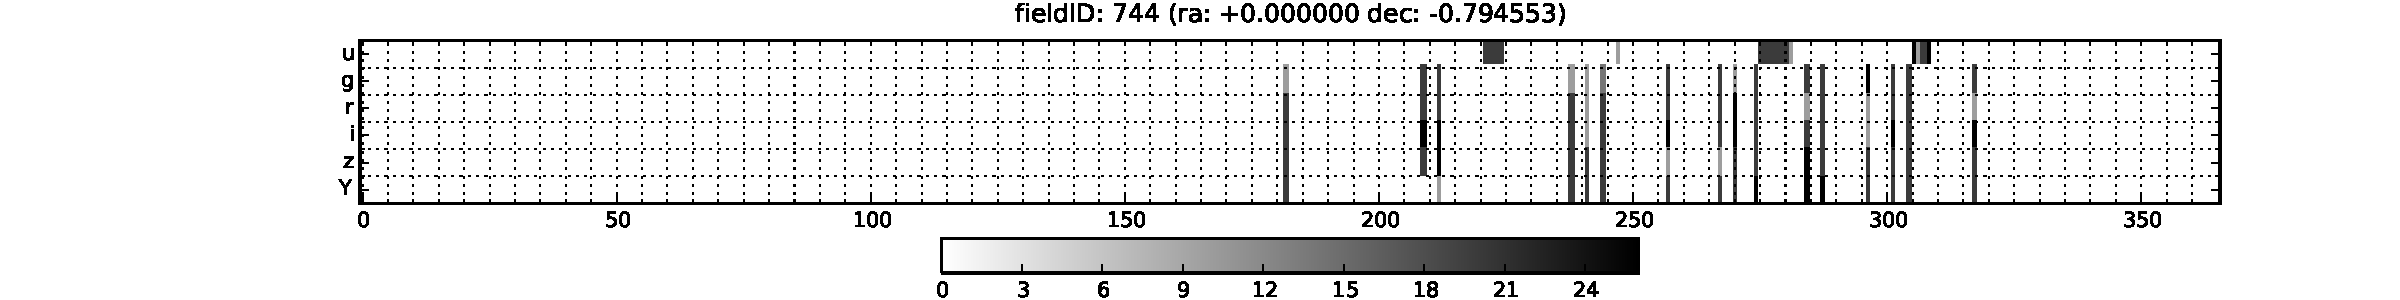
\includegraphics[width=\textwidth]{figs/supernova/fig_firstSeason_0}
        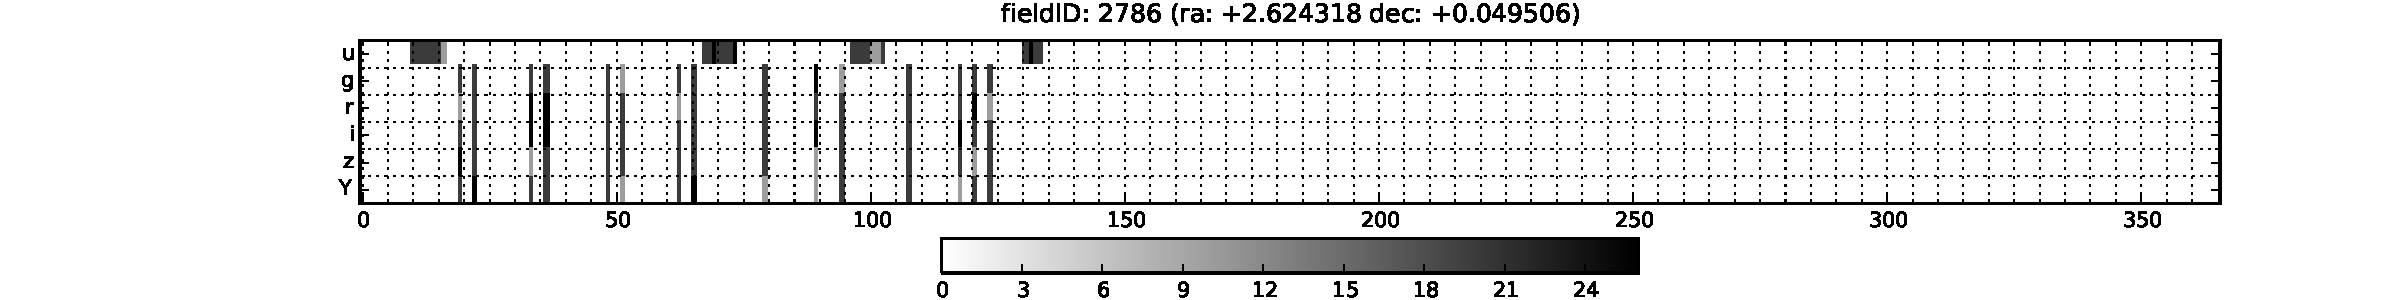
\includegraphics[width=\textwidth]{figs/supernova/fig_firstSeason_1}
        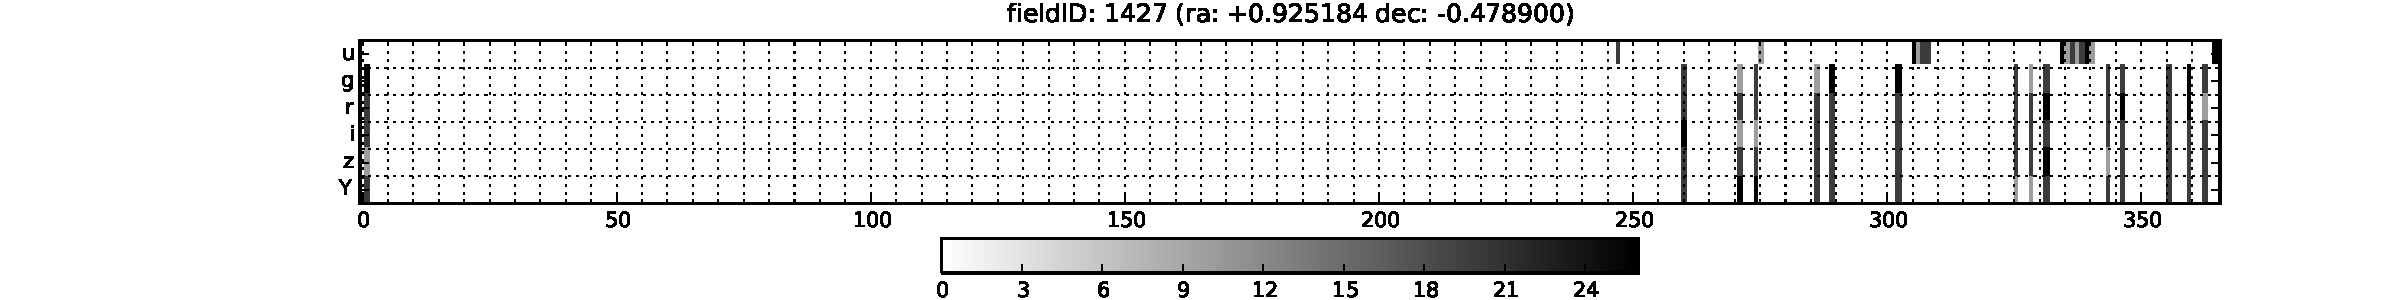
\includegraphics[width=\textwidth]{figs/supernova/fig_firstSeason_2}
        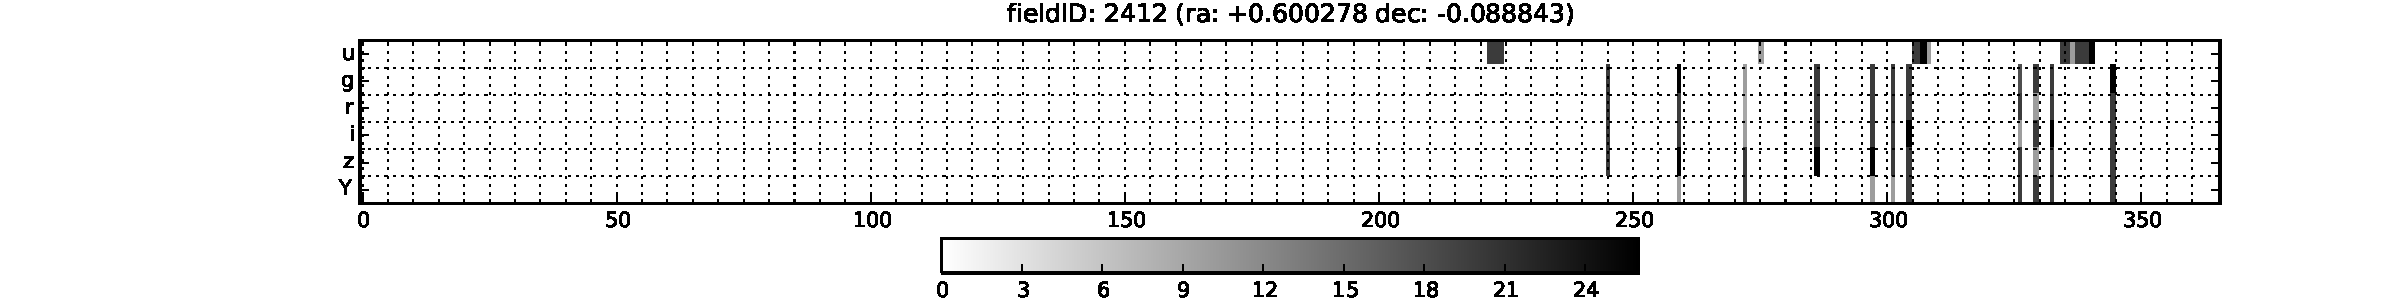
\includegraphics[width=\textwidth]{figs/supernova/fig_firstSeason_3}
        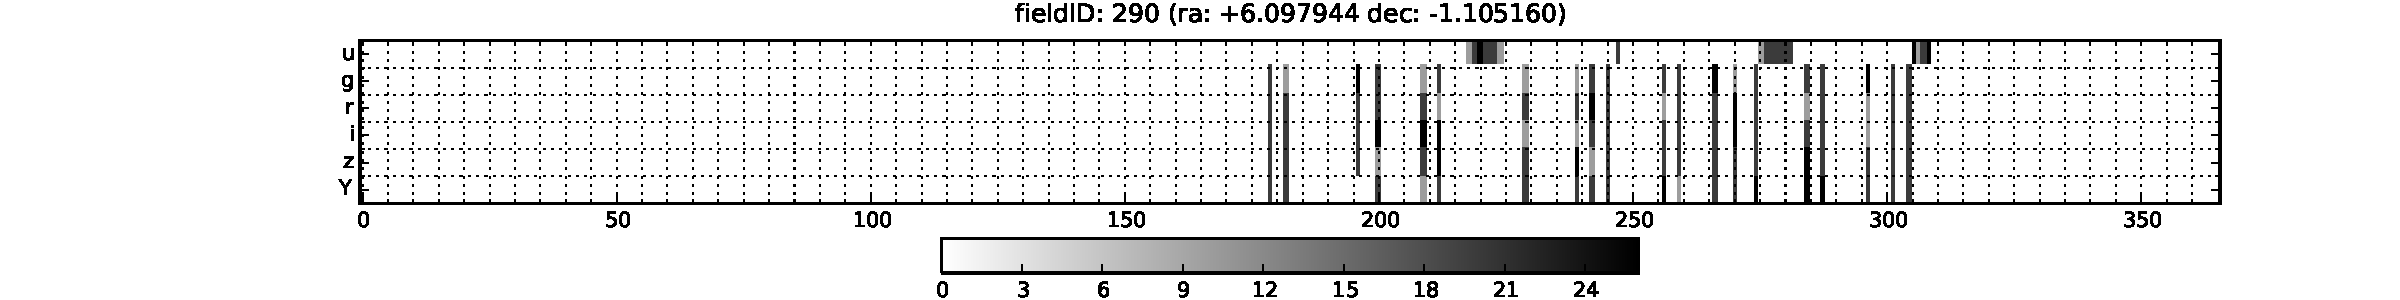
\includegraphics[width=\textwidth]{figs/supernova/fig_firstSeason_4}
    \end{minipage}
\label{fig:opsimSummary}
\caption{Include 1) an example of Type Ia Light Curve, 2) an example of Type II, 3) the number of SNR as a function of
redshift}
\end{figure*}


% --------------------------------------------------------------------

\subsection{OpsSim Analysis}
\label{sec:keyword:analysis}

{\bf Motivation and description:}

As noted above the scientific goal of characterizing SNe is to a large extent
dependent on how well the light curves of individual SNe are sampled in
time and filters. To study this, we re-index the OpsSim output on spatial
locations rather than use the temporal index. There are different methods (which will be merged), and here we will first illustrate this in terms the cadence in an example LSST field.
Our goal for observing strategy is to obtain 7-10 epochs spread over 50 days or so for more than one filter (we will quantify the mininum filters later in the Section). This will allow to increase the number of SNe at low red-shift (e.g. z$<$ 1) and to distinguish SN Ia from other types of SNe.

{\bf Analysis Results:}
We analyzed the Opsim output of the  baseline observing stragety (see Section 2.2). 
We used the file of $``$enigma_1189_sqlite.db$''$ {\footnote {http://ops2.tuc.noao.edu/runs/}}, and 
We made our analysis into with two seperate data sets; one with Deep Drilling fields and the other one with main survey.

\begin{figure}[tbh!]
\vskip -1.3in
%\includegraphics[angle=0,width=0.99\hsize:,clip]{figs/SNIaLCopsim.pdf}
\vskip -1.3in
\caption{Light curves of Supernova Type Ia generated using Deep Drilling Survey of the OpSim output in 6 different bands
}
\label{fig:SNIaLCopsimdeep}
\end{figure}



\begin{figure}[tbh!]
\vskip -1.3in
%\includegraphics[angle=0,width=0.99\hsize:,clip]{figs/SNIaLCopsim.pdf}
\vskip -1.3in
\caption{Light curves of Supernova Type Ia generated using Main Survey of the OpSim output in 6 different bands
}
\label{fig:SNIaLCopsimmain}
\end{figure}



%OpSim analysis: how good would the default observing strategy be, at
%the time of writing for this science project?



% --------------------------------------------------------------------

\subsection{Suggestion of Rolling-Cadence and its OpSim Run}
\label{sec:keyword:discussion}

Discussion: what risks have been identified? What suggestions could be
made to improve this science project's figure of merit, and mitigate
the identified risks?

{\bf Rolling-Cadence:} As mentioned above, our goal for observing strategy optimized for SN cosmology
is to obtain 7-10 epochs spread over 50 days or so for more than one filter. We suggest to change the filter 
every day and LSST can choose a part of sky which has the best airmass, centered on Zenith.
LSST will observe about 1/3 of visible sky per day (to be confirmed). LSST can observe the same part of sky for 6 days 
with 6 filters, and repeat 9 times for the same field. This observing strategy will result in 54 visits (with 6 different filters) for the same field. We repeat the same for Field 2 which takes another 54 days. Then observe Field 3 for another 54 days.

\begin{figure}[tbh!]
\vskip -1.3in
%\includegraphics[angle=0,width=0.99\hsize:,clip]{figs/SNIaLCopsim.pdf}
\vskip -1.3in
\caption{Predictions of Light curves of Supernova Type Ia using Rolling-Cadence.
}
\label{fig:SNIaLCopsimmainnew}
\end{figure}



\begin{itemize}
\item Intrinsic Dispersion, environmental effects, newer analysis methods
\item Follow-up procedures: What is feasible? Where will our training samples for classification and light curve models come from (other experiments, our own 
sub-samples with spectroscopic follow-up?), spectroscopic follow-up of host galaxies. Can hosts be identified?
\item `Systematics': In what ways will the real data not match the assumptions made in analysis. Having a large sample of SN, to understand the astrophysics would be useful for this. 
\end{itemize}


% ====================================================================

\navigationbar


% --------------------------------------------------------------------

\chapter[Deep Drilling Fields]{Drilling Deep: Options for a Small Number of Enhanced Observation
Fields}
\label{chp:deepdrilling}

\noindent {\it
Niel Brandt, Lynn Jones
}

% Introduce, with a very broad brush, this chapter's science projects,
% and why it makes sense for them to be considered together.

% Individual sections go below, one science project per section, one
% section per file.
% --------------------------------------------------------------------

% \input{DDsection1}

% --------------------------------------------------------------------

% \input{DDsection2}

% --------------------------------------------------------------------


% --------------------------------------------------------------------

\chapter[Special Surveys]{Special Surveys}
\def\chpname{specialsurveys}\label{chp:\chpname}

Chapter editors: 
\credit{dnidever},
\credit{knutago}.

% Confirmed leads for LMC/SMC: Knut Olsen, David Nidever

% Confirmed leads for special surveys:

% --------------------------------------------------------------------

\section{Introduction}
\label{sec:specials:intro}

% Introduce, with a very broad brush, this chapter's science projects,
% and why it makes sense for them to be considered together.

The four main LSST science themes, as defined by the Science Book, drive the design of LSST's main Wide-Fast-Deep survey.  However, it has always been recognized that many important scientific projects, including some that are highly relevant to LSST's main science themes, are not well served by the areal coverage and/or cadence constraints placed on the WFD survey.  The LSST Project thus set aside a nominal 10\% of the observing time to serve what are collectively called ``special surveys''.  In addition, the LSST commissioning period may be available for use by special programs.  Projects that will certainly make use of this 10\% time not dedicated to the WFD survey include the Deep Drilling fields and Galactic Plane surveys described separately in this paper, as well as any survey wishing to observe at declinations below $-60^\circ$, such as the Magellanic Clouds.  These special programs heavily oversubscribe the nominal 10\% of time assigned to them.  It is of thus critical importance for these programs to define compelling science cases, clearly justify their observing requirements, and derive metrics to quantify the performance of a given schedule for the program.  An extra degree of freedom that these special surveys


As mentioned previously, the Deep Drilling and Milky Way plane surveys are described separately in this paper.  In this section, we describe the goals of two special surveys designed to serve scientific goals related to the Magellanic Clouds.  Descriptions of other special surveys, including candidate commissioning programs, are welcome here.


% Add sections below, one science investigation per section, one
% section per file.
% --------------------------------------------------------------------

% ====================================================================
%+
% NAME:
%    section-name.tex
%
% ELEVATOR PITCH:
%    Explain in a few sentences what the relevant discovery or
%    measurement is going to be discussed, and what will be important
%    about it. This is for the browsing reader to get a quick feel
%    for what this section is about.
%
% COMMENTS:
%
%
% BUGS:
%
%
% AUTHORS:
%    David Nidever (@dnidever)
%    Knut Olsen (@knutago)
%-
% ====================================================================

\section{ The Magellanic Clouds }
\def\secname{MCs}\label{sec:\secname}

\noindent{\it David L. Nidever, Knut Olsen} % (Writing team)

% This individual section will need to describe the particular
% discoveries and measurements that are being targeted in this section's
% science case. It will be helpful to think of a ``science case" as a
% ``science project" that the authors {\it actually plan to do}. Then,
% the sections can follow the tried and tested format of an observing
% proposal: a brief description of the investigation, with references,
% followed by a technical feasibility piece. This latter part will need
% to be quantified using the MAF framework, via a set of metrics that
% need to be computed for any given observing strategy to quantify its
% impact on the described science case. Ideally, these metrics would be
% combined in a well-motivated figure of merit. The section can conclude
% with a discussion of any risks that have been identified, and how
% these could be mitigated.

%A short preamble goes here. What's the context for this science
%project? Where does it fit in the big picture?
The Magellanic Clouds have always had outsized importance for astrophysics.  They are critical steps in the cosmological distance ladder, they are a binary galaxy system with a unique interaction history, and they are laboratories for studying all manner of astrophysical phenomena.  They are often used as jumping-off points for investigations of much larger scope and scale; examples are the searches for extragalactic supernova prompted by the explosion of SN1987A and the dark matter searches through the technique of gravitational microlensing.  More than 17,000 papers in the NASA ADS include the words ``Magellanic Clouds'' in their abstracts or as part of their keywords, highlighting their importance for a wide variety of astronomical studies.

An LSST survey that did not include coverage of the Magellanic Clouds and their periphery would be tragically incomplete.  LSST has a unique role to play in surveys of the Clouds.  First, its large $A\Omega$ will allow us to probe the thousands of square degrees that comprise the extended periphery of the Magellanic Clouds with unprecedented completeness and depth, allowing us to detect and map their extended disks, stellar halos, and debris from interactions that we already have strong evidence must exist (REFS).  Second, the ability of LSST to map the entire main bodies in only a few pointings will allow us to identify and classify their extensive variable source populations with unprecedented time and areal coverage, discovering, for example, extragalactic planets, rare variables and transients, and light echoes from explosive events that occurred thousands of years ago (REFS).  Finally, the large number of observing opportunities that the LSST 10-year survey will provide will enable us to produce a static imaging mosaic of the main bodies of the Clouds with extraordinary image quality, an invaluable legacy product of LSST.

We propose two distinct mini-surveys to meet the goals of LSST Magellanic Clouds science:
\begin{itemize}
\item A mini-survey covering the 2700$\deg^2$ with $\delta < -60$ to the standard LSST single-exposure depth and to stacked depths of XXX, with cadence sufficient to detect and measure light curves of RR Lyrae stars 
\item A mini-survey covering $\sim$250$\deg^2$ of the main bodies of the Clouds with cadence sufficient to detect exoplanet transits and other variable objects; a subset of these images should be taken with seeing of $0.5\arcsec$, with stacked depth reaching the confusion limits in the Clouds
\end{itemize}

Figure X shows a rough map of the proposed mini-surveys.  
% Need the figure and caption
These surveys will support several important scientific goals:
\begin{enumerate}
\item What are the stellar and dark matter mass profiles of the Magellanic Clouds?  Map extended disk, halo, debris, and streams.  Use streams as probes of total mass profile.  RR Lyrae give potential for three-dimensional stellar profile.
\item What is the satellite population of the Magellanic Clouds?  Discovery of dwarfs by DES and other surveys illuminating for understanding distribution of dark matter subhalos and how galaxies form in them (REFS)
\item What are the internal dynamics of the Magellanic Clouds?  Proper motions from HST and from the ground (REFS) have measured the bulk motions of the Clouds and have, in combination with spectroscopy, begun to unravel the three dimensional internal dynamics of the Clouds...
\item How do exoplanet statistics in the Magellanic Clouds compare to those in the Milky Way?  Lund calculation shows can measure transits of Jupiter-like planets, Clouds are lower metallicity environment
\item Identify and characterize the variable star and transient population of the Clouds.  Population studies, linking to star formation and chemical enrichment histories, etc, from Szkody et al. DD white paper.
\item Light echoes from supernovae and explosive events.  Echoes can give view of such events unavailable by any other means, ref. papers by Rest et al.
\end{enumerate}

% Convert list to short sections to provide background on these topics?

%David's text
Two main overarching science themes:
\begin{enumerate}
\item {\bf Galaxy formation evolution}: The study of the formation and evolution of the Large and Small
  Magellanic Clouds (LMC and SMC, respectively), especially their interaction with each other and the Milky Way.
  The Magellanic Clouds (MCs) are a unique local laboratory for studying the formation and evolution of
  dwarf galaxies in exquisite detail.  LSST's large FOV will be able to map out the three-dimensional
  structure, metallicity and kinematics in great detail.
\item {\bf Stellar astrophysics \& Exoplanets}:  The MCs have been used for decades to study stellar
  astrophysics, microlensing and other processes.  The fact that the objects are effectively all at a single
  known distance makes it much easier to study them than in, for example, the Milky Way.  LSST will extend
  these studies to fainter magnitudes, higher cadence, and larger area.
\end{enumerate}

Many different types of objects and measurements with their own cadence ``requirements'' will fall into
these two broad categories (with some overlap).  These will be outlined in the next section.

A very important aspect of the ``galaxy evolution'' science theme is not just the cadence but also the
sky coverage of the Magellanic Clouds ``mini-survey''.  A common misunderstanding is that the MCs only
cover a few degrees on the sky.  That is, however, just the central regions of the MCs akin to the thinking
of the Milky Way as the just the bulge.  The full galaxies are actually much larger with LMC stars
detected at $\sim$21$^{\circ}$ ($\sim$18 kpc) and SMC stars at $\sim$10$^{\circ}$ ($\sim$11 kpc) from their
respective centers.  The extended stellar debris from their interaction likely extends to even larger
distances.  Therefore, to get a complete picture of the complex strucure of the MCs will require a
mini-survey that covers $\sim$2000 deg$^2$.  At this point, it not entirely clear how to include this
into the metrics.  Note, that for the second science case this is not as much of an issue since the large
majority of the relevant objects will be located in the high-density, central regions of the MCs.


% --------------------------------------------------------------------

\subsection{Target measurements and discoveries}
\label{sec:keyword:targets}

%Describe the discoveries and measurements you want to make.
%
%Now, describe their response to the observing strategy. Qualitatively,
%how will the science project be affected by the observing schedule and
%conditions? In broad terms, how would we expect the observing strategy
%to be optimized for this science?

\begin{enumerate}

\item Deep Color Magnitude Diagrams
%  -Deep CMDs, just a matter of number of visits
%  -do the full SMASH (and relevant DES area) with full spatial coverage, at least to SMASH depths, smaller
%  number of epochs, ~5 sigma at gri~25
% Knut thoughts: I think we want to make sure that we get 1 mag below old turnoff out to 100 kpc in ugriz with 10sigma precision, i.e. ugriz~25


\item Proper Motions
%-Proper Motions, cadence not as much of an issue, just more epochs
%  bulk proper motion
%  LMC spiral motion, streaming motions
%  internal velocity dispersion

%\item Parallaxes
%-Parallaxes, also mostly a function of nubmer of epochs
%  bulk distances
%  internal distance spread

\item Variable stars

%-Variables, RR Lyrae, Cepheids might be too bright, dwarf cepheids/scuti good, many more of them.
%   especially good for getting the 3D structure (out to large distances) of the MCs
%   -eclipsing binaries (get very accurate distances, see OGLE paper), pulsating WDs, CVs, T Tauri stars

\item Transients
%-Transients, dwarf novae

\item Transiting Exoplanets
% -Transiting planets

\item Astrometric binaries
%-Astrometric binaries

\item Gyrochronology
%-Gychronology, need to get periods of the dwarfs, gives age information

\item Astroseismology
%-Astroseismology, dwarfs/giants, giants vary by a couple percent and on "longer" timescales, but
%    probably too bright for LSST, OGLE probably has best data for those. however LSST might be able to do
%    asteroseismology of giants to larger distances, measure masses/ages of halo giants!
%    dwarfs are harder because they vary less and need more higher frequency observations

\end{enumerate}

% --------------------------------------------------------------------

\subsection{Metrics}
\label{sec:keyword:metrics}

Quantifying the response via MAF metrics: definition of the metrics,
and any derived overall figure of merit.


% --------------------------------------------------------------------

\subsection{OpSim Analysis}
\label{sec:keyword:analysis}

OpSim analysis: how good would the default observing strategy be, at
the time of writing for this science project?


% --------------------------------------------------------------------

\subsection{Discussion}
\label{sec:keyword:discussion}

Discussion: what risks have been identified? What suggestions could be
made to improve this science project's figure of merit, and mitigate
the identified risks?


% ====================================================================

\navigationbar



\section{Short Exposure Survey- Introduction }

The current LSST requirements stipulate a minimum exposure time of 5 seconds, with an expected default exposure time of 15 seconds. This document advocates for decreasing the minimum exposure time requirement from 5 to 0.1 seconds. This would increase the dynamic range for bright sources (compared to the default 15 sec time) by about 5 magnitudes, to a total of 13 astronomical magnitudes (where dynamic range is the difference between the brightest unsaturated source and the faintest point source detectable at 5 sigma). This is a large factor, and would enable a wide range of science goals, outlined below. One interesting aspect of this is that it would allow us to operate the LSST system during twilight times that would otherwise saturate the array due to background sky brightness. This would allow a number of the goals described below to be carried out without impacting the primary survey by conducting observations during twilight sky conditions that would saturate the array at longer exposure times. 

Since the twilight sky brightness is an important factor discussed below, we provide here a very brief outline of the temporal evolution of the background sky brightness. 

Tyson and Gal (1993) provide a simple framework that serves our purposes well. They provide observational data as well as a simple model for the evolution of twilight sky brightness. Figure 1 from that paper is included below. They show that a good model for the sky brightness evolution is given by an exponential with 
$\log_{10}(S)=(k/\tau)t+C$, 
where S is the sky brightness in electrons per pixel per second, C is the dark sky background, k = (10.6 minutes)$^{-1}$  is a universal (band-independent) timescale during which the sky�s surface brightness changes by a factor of ten (at latitude $-$30 degrees), and $\tau$ is a season-dependent factor that ranges from 1.0 at the equinox to 1.07 in austral winter and 1.20 in austral summer. So the rule of thumb is that we should expect it to take 4.25 minutes for the sky background to change by one magnitude per square arc sec. (In what follows we'll ignore the increased twilight time in summer and winter.)

For current generation typical astronomical camera systems that take over a minute to read out, this 4.2 minute time scale means that only a handful of images can be obtained during twilight time. But for the LSST camera with a 2 second readout time, we can obtain hundreds of short exposures during twilight. Even if we are limited to a 15 second cadence due to thermal stability or data transfer limitations there is a large amount of time opened up that we can use. 

What do we stand to gain in operational time with shorter exposures? If the standard survey terminates taking 15 second exposures due to some sky brightness criterion, by shifting to 0.1 sec images at that point we will have changed the sky flux per pixel by 2.5 $\log_{10}(150)$ = 5.4 magnitudes. This brings us back into a high dynamic range regime, as described below. 

\begin{figure}[htbp]
\begin{center}
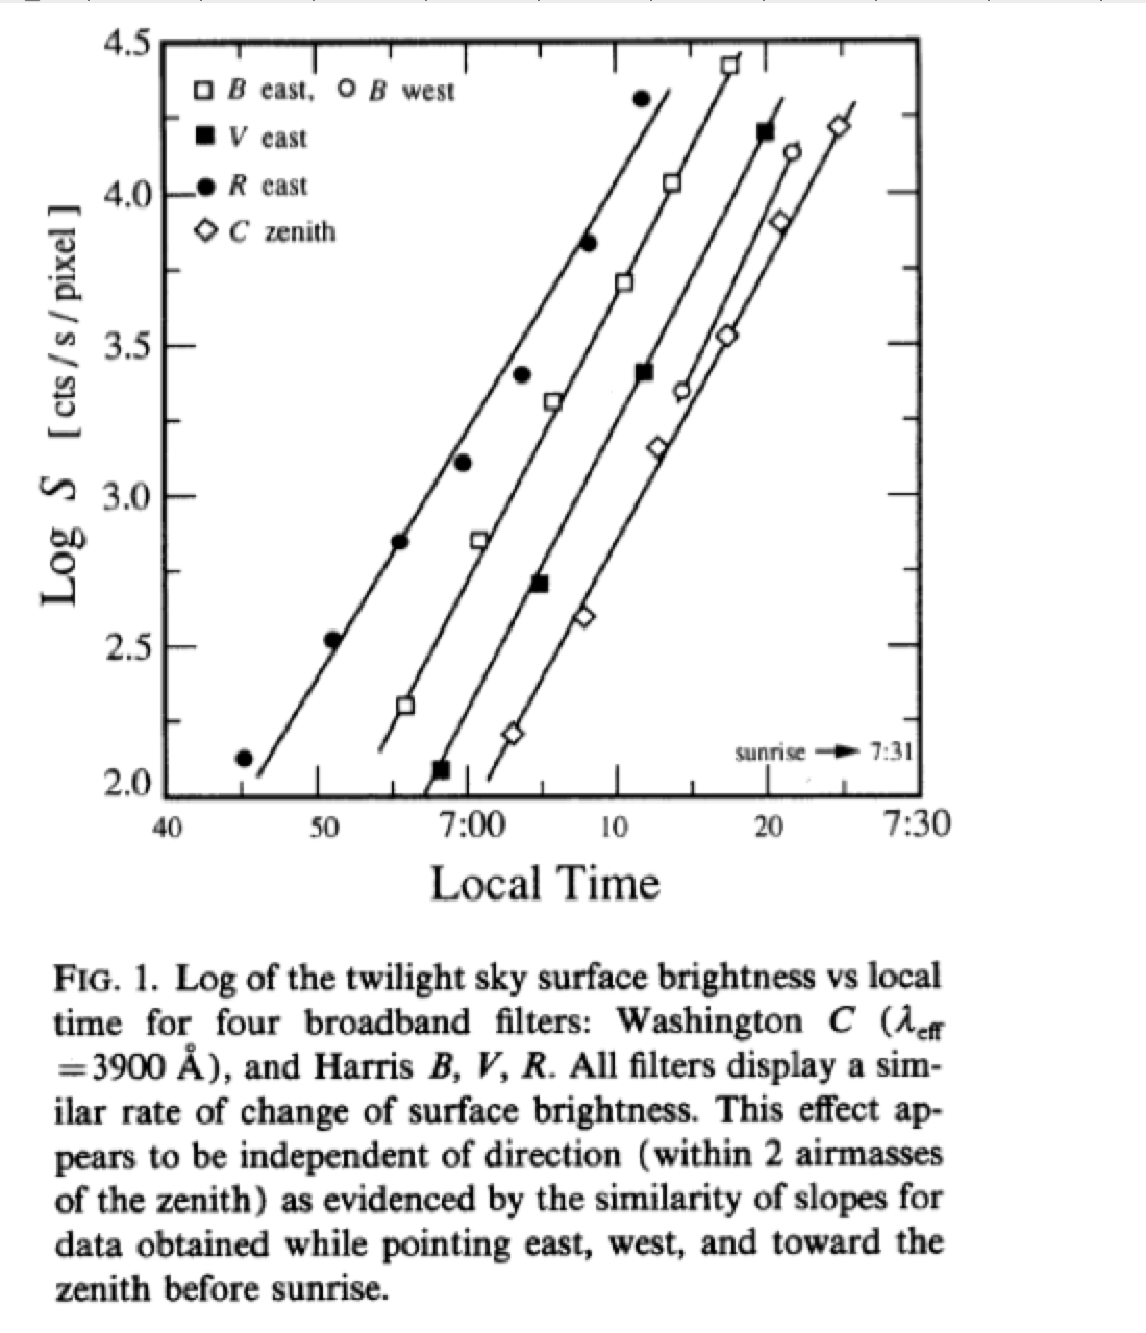
\includegraphics[width=6in]{figs/Stubbs_Fig1.pdf}
\caption{(reproduced from Tyson et al, 1993). This plot shows that the sky brightness changes by one magnitude in a 4.2 minute interval, essentially independent of passband.}
\label{default}
\end{center}
\end{figure}

Figure 2 illustrates the principles that underpin this proposal. LSST is a unique combination of hardware and software, that will deliver reliable catalogs of both the static and the dynamic sky. By pushing towards shorter integration times we can greatly expand the scientific reach of the system. 

The dynamic range in magnitudes that we can achieve for a given integration time depends on the sky background, the read noise, and the full well depth per pixel. We will adopt a typical value of 100Ke for the full well depth, but the arguments presented below are essentially independent of this value. The dynamic range in magnitudes is limited on the bright end by the point source whose PSF peak exceeds full well, and on the faint end by the 5$\sigma$ point source sensitivity, which depends on sky brightness per pixel. So we are squeezed between the two parameters of full well depth and sky background. 

\begin{figure}[htbp]
\begin{center}
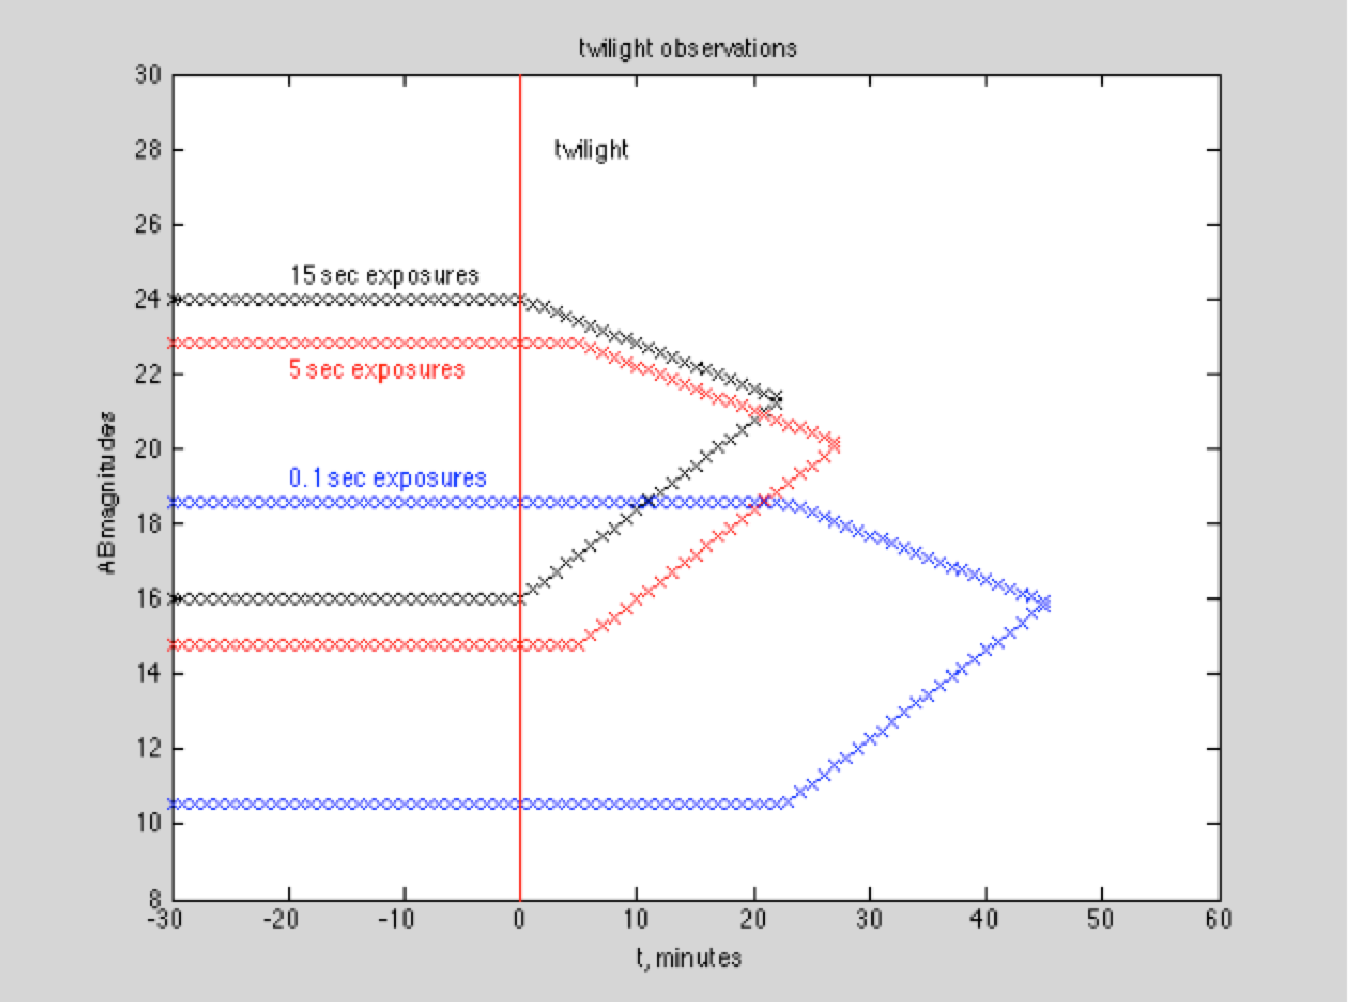
\includegraphics[width=6in]{figs/Stubbs_Fig2.pdf}
\caption{Twilight dynamic range. As we enter morning twilight time, the increasing sky brightness requires brighter sources for 5 sigma detection, and also limits unsaturated objects to increasingly fainter sources. Eventually the gap between these goes to zero. But operating at shorter exposure times allows us to push useful survey operations into brighter twilight time, and also to increase the dynamic range of the LSST survey products. The black lines correspond to 15 second integrations (nominally in the r band), the red lines to 5 second exposures, and the blue curves to 0.1 second exposures. The upper lines in each case represent the 5 sigma point source detection threshold while the lower line corresponds to the source brightness that produces saturation in the peak pixel of the PSF. Adding shorter exposure times increases our dynamic range in flux, and adds valuable observing time.}
\label{default}
\end{center}
\end{figure}

The 5 sigma limiting flux scales as the square root of the sky brightness, while the saturation flux decreases linearly as sky brightness increases. So the two curves in Figure 2 have slopes that differ by a factor of two. Operating during bright-sky time with short exposures adds about 20 minutes of observing per twilight, or 40 minutes per night. This is a non-trivial resource!

Figure 2 shows one reason why it is not advantageous to go below 0.1 second exposures- we would lose the overlap between a twilight survey and the standard LSST object catalog. 

Having set the stage for the opportunity to operate at shorter exposure times either during dark sky time, or during twilight, or both, we now describe some of the scientific motivations for doing so. 

\subsection{Science Drivers for Shorter Exposures}

\subsubsection{Discovery space at short time scales.} 

LSST is a time domain discovery machine. It is hard to anticipate the importance of being able to detect astronomical variability on short time scales. By extending the time domain sensitivity to phenomena with a characteristic time of less than 5 seconds, we will have added 1.5 orders of magnitude in time domain sensitivity. 

Taking short exposures does not necessarily imply a requirement on fast image cadence. Periodic variability can be readily detected and characterized with a succession of short images that do not satisfy the Nyquist criterion, as long as we know the time associated with each data point to adequate accuracy. But it does seem appropriate to investigate the maximum possible rapid-fire imaging rate for LSST, presumably limited by either data transfer bottlenecks or by thermal issues within the camera. 

\subsubsection{Distances to Nearby SN Ia- an essential ingredient in using supernovae to probe dark energy.}

The determination of the equation of state parameter of the Dark Energy using type Ia supernovae entails measuring the redshift dependence of the luminosity distances to objects over a range of redshifts. The low end of this redshift range is limited by peculiar velocities to considering supernovae at redshifts z$>$0.01. At this distance (distance modulus of 
$\mu$ =33) the peak brightness of a type Ia supernova is r=15 and exceeds the expected LSST point source saturation limit. 

Moreover, the rate on the sky of these bright nearby supernovae is so low that in the standard cadence we don�t expect to obtain well-sampled multiband light curves for them. But we will discover many of them on the rise. Using twilight time with short exposures to obtain appropriate temporal and passband coverage will allow us to extend the LSST SN Hubble diagram across the entire redshift range of 0.01 to 1. 

It is vitally important that we obtain these nearby-SN light curves on the same photometric system, reduced with the same data reduction pipeline, as the distant sample. This means we really must use the LSST instrument and software in order to avoid systematic errors arising from differences in photometric systems or algorithmic issues. 

We stress that this twilight SN followup campaign can be accomplished without impacting the main survey, during the roughly 20 minutes per night of twilight that would otherwise unusable at the default exposure time. We would use the brighter twilight time to obtain pointed observations on nearby supernovae, motivated by the importance of photometric uniformity described above. 

\subsubsection{A Bright Star Survey for Galactic Science.}

We could also use the added twilight time to conduct a bright star survey, and the precise astrometry and photometry from LSST can then be used in conjunction with archived data ranging from 11th to 27th AB magnitudes. This short-exposure domain would extend the LSST dynamic range in fluxes by two orders of magnitude, towards the bright end. Moreover, obtaining precise positions, fluxes and variability at these brighter magnitudes would greatly increase the overlap with the historical archive of astronomical information, including from digitized plate data. We would be able to obtain astrometric and color information to high precision, as well time series for variability studies. 

An example of an application to Milky Way structure studies comes from RR Lyrae variable stars. With a saturation magnitude of around 16th in the standard LSST survey, RR Lyrae closer than 20 kpc will be saturated in the standard LSST images. So we will lose nearly all Galactic RR Lyrae. Extending the survey�s bright limit to 11th magnitude will allow us to collect light curves for RR Lyrae beyond $\sim$ 100 parsecs, collecting essentially all Southern hemisphere Galactic RR Lyrae.

Another application for stellar population studies is measuring the fraction of binary stars as a function of stellar type, metallicity, age and environment. By conducting a variability survey in the 11-18 magnitude range we can capitalize on temperature and metallicity data already in hand for many of these objects. 

Another application of a bright star survey would be to search for planetary transits in the magnitude range appropriate for radial velocity followup observations using 30 meter class telescopes. For high dispersion spectrographs at the 4m aperture class, most targets are currently around 8th magnitude, so we should expect 30m telescopes to attain similar radial velocity precisions for sources of magnitude  8 + 5log(30/4) = 12. By going to shorter exposures we obtain almost an hour�s additional observing time per night when these sources don�t saturate, whereas they are far beyond saturation in the default 15 second LSST survey images. 

A typical (r$-$K) color between SDSS and 2MASS is r$-$K=3. The 2MASS catalog is complete down to K$\sim$14 which corresponds to r$\sim$17. So most 2MASS stars will be saturated in the standard LSST 15 second observations. A bright star survey will allow a multiband match to the 2MASS data, as well as an astrometric comparison between the two catalogs. 

Finally, the apparent magnitude of solar system objects depends on their distance from us and from the sun, as well as illumination and observation geometry. Extending the bright limit will allow us to track asteroid positions as they approach opposition.  

\subsection{Counterarguments}

\subsubsection{What About Scintillation Effects?}

Short exposure times suffer from scintillation effects. An estimate for uncertainty due to scintillation is provided by 
\url{http://astro.corlan.net/gcx/scint.txt}. For a 0.1 second integration we expect a fractional flux uncertainty of  0.15 at 2 airmasses and 0.043 at 1 airmass, for a 10 cm aperture. Scaling this up to the 8.5m aperture of LSST by a factor D$^{2/3}$ predicts fractional flux variations of below one percent, even at two airmasses, for a 0.1 second exposure. So scintillation should not impact our ability to make precision measurements of flux and position.  

\subsubsection{What about just doing this with smaller telescopes?}

A possible counter-argument to the proposal of allowing for shorter exposure times is that much of this can be done with smaller telescopes. But it�s important to bear in mind that LSST is a system, and the data reduction and dissemination tools are as important as the hardware. We intend to deliver accessible, high-quality, well-calibrated photometry on a common photometric system and correspondingly good positions. If we do so from a co-added point source depth of 27th to the short-exposure bright limit of 11th magnitude we will span over six decades in flux on a well-calibrated flux scale. We would also have the ability to study astrophysical variability on time scales from 0.1 second to 10 years, which is nine decades in the time domain. This combination of temporal and flux dynamic range would be a truly remarkable  achievement, and would yield science benefits far beyond the illustrative examples provided above. Much of this discovery space is enabled by going to shorter exposures. 
 
\subsection{Proposed Implementation and Impacts}

The implementation of this would simply entail taking short-exposure images during twilight time that would otherwise go unused. The data rate would go up, and the number of shutter cycles per night would also increase. 
%
%\section{References}
%
%Tyson and Gal, An Exposure Guide for Taking Twilight Flats with Large Format CCDs, AJ {\bf 105}, 1026 (1003). 




% --------------------------------------------------------------------

% \input{commissioning.tex}

% --------------------------------------------------------------------

\navigationbar


% --------------------------------------------------------------------

\chapter[Tensions and Trade-offs]{Tensions and Trade-offs}
\def\chpname{tradeoffs}\label{chp:\chpname}

\noindent {\it
...
}

Discussion and conclusions chapter, at the end, highlighting the
issues that we will need to figure out. Possible topics include the
cost/benefit tradeoffs between competing objectives.


% --------------------------------------------------------------------

\bibliographystyle{apj}
\bibliography{references}

% --------------------------------------------------------------------

\end{document}

% ====================================================================
